\documentclass[10pt]{article}

\usepackage[pdftex]{graphicx} 
  \usepackage{pgfplots}
\pgfplotsset{compat=newest}
%% the following commands are needed for some matlab2tikz features
\usetikzlibrary{plotmarks}
\usetikzlibrary{arrows.meta}
\usepgfplotslibrary{patchplots}
\usepackage{grffile}
\usepackage{amsmath}


%\usepackage{fullpage}
\usepackage[top=1in, bottom=1in, left=0.8in, right=1in]{geometry}
\usepackage{multicol}
%\usepackage{wrapfig}
%\usepackage{listings}
\usepackage{caption}
\usepackage{subcaption}
\usepackage{hyperref}
\usepackage{xcolor}
%\usepackage{soul}
\usepackage{tikz}

\definecolor{lightblue}{rgb}{.80,.9,1}
\newcommand{\hl}[1]
    {\par\colorbox{lightblue}{\parbox{\linewidth}{#1}}}

\newcommand{\defn}{\stackrel{\textrm{\scriptsize def}}{=}}

\setlength{\columnsep}{0.1pc}

\title{gSGN Wave Speeds and The Dam-break Problem.}
%\author{Christopher Zoppou -- \texttt{christopher.zoppou@anu.edu.au}, Dimitrios Mitsotakis -- \texttt{dmitsot@gmail.com}, Stephen Roberts -- \texttt{stephen.roberts@anu.edu.au}, Jordan Pitt}

% TIME ON EVERY PAGE AS WELL AS THE FILE NAME
\usepackage{fancyhdr}
\usepackage{currfile}
\usepackage[us,12hr]{datetime} % `us' makes \today behave as usual in TeX/LaTeX
\fancypagestyle{plain}{
\fancyhf{}
\rfoot{\emph{\footnotesize \textcopyright  gSGN Letter to Dimitrios Mitsotakis by Jordan Pitt, Chris Zoppou and Stephen Roberts.}
 \\ File Name: {\currfilename} \\ Date: {\ddmmyyyydate\today} at \currenttime}
\lfoot{Page \thepage}
\renewcommand{\headrulewidth}{0pt}}
\pagestyle{plain}

\begin{document}

\maketitle

\vspace{-0.3in}
\noindent
\rule{\linewidth}{0.4pt}

%-------------------------------------------------
%\section{Introduction}
%-------------------------------------------------
Hello Dimitrios, I have adapted the $\text{FDVM}_2$ method in \cite{Zoppou-etal-2017} to solve the gSGN (generalised Serre-Green-Naghsi) equations from \cite{Clamond-Dutykh-2018-237}. 

The $\text{FDVM}_2$ method uses a second-order finite difference approximation to solve the elliptic equation that related the new conserved quantity $G$ to the primitive variable $u$, and a finite volume method with second-order Runge-Kutta time stepping to obtain a fully second order method. I have been able to demonstrate convergence to forced solutions and the ability of the method to reproduce the analytic solutions for well known members of this family of equations captureed by the gSGN; the dambreak problem for the SWWE and the soliton solution for the Serre equations.

To remind you, the gSGN equations and its reformulation into a conservative form are here.

%-------------------------------------------------
\section{gSGN - generalised Serre-Green-Naghdi equations}
%-------------------------------------------------
\cite{Clamond-Dutykh-2018-237} derived the following generalised version of the Serre-Green-Naghdi equations:

\begin{subequations}
	\begin{gather}
	\dfrac{\partial h}{\partial t} + \dfrac{\partial (uh)}{\partial x} = 0
	\label{eq:gSGNh}
	\end{gather}
	\begin{gather}
	\dfrac{\partial (uh)}{\partial t} + \dfrac{\partial }{\partial x} \left( u^2h + \dfrac{gh^2}{2} + \frac{1}{3} h^2 \Gamma \right)= 0
	\label{eq:gSGNuh}
	\end{gather}
	\begin{multline}
	\dfrac{\partial}{\partial t}\left[\frac{1}{2}hu^2 + \dfrac{1}{2}\left(1 + \frac{3}{2}\beta_1\right) h^3 \dfrac{\partial u}{\partial x}\dfrac{\partial u}{\partial x} + \frac{1}{2}gh^2\left(1 + \frac{1}{2}\beta_2 \dfrac{\partial h}{\partial x} \dfrac{\partial h}{\partial x}\right) \right] \\
	\dfrac{\partial}{\partial x}\left[uh\left(\frac{1}{2}u^2 + \dfrac{1}{2}\left(1 + \frac{3}{2}\beta_1\right)h^2\dfrac{\partial u}{\partial x}\dfrac{\partial u}{\partial x} + gh\left(1 + \frac{1}{4}\beta_2\dfrac{\partial h}{\partial x}\dfrac{\partial h}{\partial x} \right)   + \frac{1}{3} h\Gamma  \right) + \frac{1}{2}\beta_2 g h^3\dfrac{\partial h}{\partial x}\dfrac{\partial u}{\partial x} \right]
	=0
	\label{eq:gSGNE}
	\end{multline}
	where
	\begin{equation}
	\Gamma = \left(1 + \frac{3}{2}\beta_1\right)h \left[\frac{\partial u}{\partial x}\frac{\partial u}{\partial x} - \frac{\partial^2 u}{\partial x \partial t} - u\frac{\partial^2 u}{\partial x^2}\right] - \frac{3}{2} \beta_2 g\left[h \frac{\partial^2 h}{\partial x^2} + \frac{1}{2} \frac{\partial h}{\partial x}\frac{\partial h}{\partial x} \right]
	\end{equation}
	\label{eq:gSGN}
\end{subequations}

Thus we have conservation of mass, momentum and energy for all values of $\beta_j$. 

From these equations the SWWE, the Serre equations and the regularised SWWE \cite{Clamond-Dutykh-2018-237} can be recovered for certain values of $\beta_1$ and $\beta_2$. Summaried in Table \ref{tab:betavalues}. 

\begin{table}
	\centering
	\begin{tabular}{c | c | c}
		Resulting Equations &$\beta_1$ & $\beta_2$  \\
		\hline 
		Serre Equations & $0$ & $0$ \\
		SWWE Equations & $-\dfrac{2}{3}$ & $0$ \\
		Regularised SWWE Equations & free variable & $\beta_1 + \dfrac{2}{3}$  \\
		Improved Dispersion Serre Equations & free variable & $\beta_1$
	\end{tabular}
	\caption{Showing various combinations of $\beta$ values and equivalent equations \label{tab:betavalues}}
\end{table}

%-------------------------------------------------
\subsection{Alternative Conservative Form of the gSGN}
%-------------------------------------------------

A major difficulty with solving the SGN is that the dispersive terms contain a mixed spatial-temporal derivative term which is difficult to handle numerically. This mixed derivative term can be rewritten  so that the Serre equations can be expressed in conservation law form, with the water depth and a new quantity as conservative variables. This reformulation allows standard techniques for solving conservation laws to be applied to the Serre equations, even though the Serre equations are neither hyperbolic nor parabolic.

Consider the Serre equations written for a horizontal bed. The flux term in the momentum equation, \eqref{eq:gSGNuh} contains a mixed spatial and temporal derivative term which is difficult to treat numerically. It is possible to replace this term  by a combination of spatial and temporal derivative terms by making the following observation
\begin{multline}
\dfrac{\partial^2}{\partial x \partial t} \left ( \frac{1}{3}\left(1 + \frac{3}{2} \beta_1\right) h^3 \dfrac{\partial u}{\partial x} \right ) =   \frac{1}{3}\left(1 + \frac{3}{2} \beta_1\right) \dfrac{\partial }{\partial t} \left ( 3h^2 \dfrac{\partial h}{\partial x} \dfrac{\partial u}{\partial x} + h^3 \dfrac{\partial^2 u}{\partial x^2} \right ) \\=  \frac{1}{3}\left(1 + \frac{3}{2} \beta_1\right)
\dfrac{\partial }{\partial x} \left ( 3 h^2 \dfrac{\partial h}{\partial t} \dfrac{\partial u}{\partial x} + h^3 \dfrac{\partial^2 u}{\partial x \partial t} \right ).
\end{multline}
Rearranging and making use of the continuity equation, \eqref{eq:gSGNh} the momentum equation, \eqref{eq:gSGNuh} becomes
\begin{multline}
\dfrac{\partial }{\partial t} \left ( u h -  \frac{1}{3}\left(1 + \frac{3}{2} \beta_1\right) \dfrac{\partial}{\partial x} \left [h^3 \dfrac{\partial u}{\partial x}  \right ] \right ) \\ + \dfrac{\partial}{\partial x} \left ( u\left[uh - \frac{1}{3}\left(1 + \frac{3}{2} \beta_1\right) \dfrac{\partial }{\partial x} \left [ h^3 \dfrac{\partial u}{\partial x} \right ]\right] + \dfrac{gh^2}{2} - \frac{2}{3}\left(1 + \frac{3}{2} \beta_1\right) h^3\dfrac{\partial u}{\partial x}\dfrac{\partial u}{\partial x}  - \frac{1}{2} \beta_2 g h^2 \left[h\frac{\partial^2 h}{\partial x^2} + \frac{1}{2}\frac{\partial h}{\partial x}\frac{\partial h}{\partial x}\right]\right ) = 0.
\end{multline}
The momentum equation can be written in conservation law form as
\begin{gather}\label{eq:G_momentum}
\dfrac{\partial G }{\partial t}  + \dfrac{\partial}{\partial x} \left ( uG + \dfrac{gh^2}{2} - \frac{2}{3}\left(1 + \frac{3}{2} \beta_1\right) h^3\dfrac{\partial u}{\partial x}\dfrac{\partial u}{\partial x}  - \frac{1}{2} \beta_2 g h^2  \left[h\frac{\partial^2 h}{\partial x^2} + \frac{1}{2}\frac{\partial h}{\partial x}\frac{\partial h}{\partial x}\right]\right ) = 0.
\end{gather}
where a new conserved quantity, $G$ is given by
\begin{gather*}
G = uh - \frac{1}{3}\left(1 + \frac{3}{2} \beta_1\right) \dfrac{\partial }{\partial x} \left ( h^3 \dfrac{\partial u}{\partial x} \right ).
\end{gather*}
This expands the conserved variable introduced by \cite{Clamond-Dutykh-2018-237}, as well as in the Serre equations \cite{Zoppou-etal-2017}. 

Thus we have the following conservation equations

\begin{subequations}
\begin{gather}
\dfrac{\partial h}{\partial t} + \dfrac{\partial (uh)}{\partial x} = 0
\label{eq:gSGN_Gh}
\end{gather}
\begin{gather}
\dfrac{\partial G }{\partial t}  + \dfrac{\partial}{\partial x} \left ( uG + \dfrac{gh^2}{2} - \frac{2}{3}\left(1 + \frac{3}{2} \beta_1\right) h^3\dfrac{\partial u}{\partial x}\dfrac{\partial u}{\partial x}  - \frac{1}{2} \beta_2 g h^2  \left[h\frac{\partial^2 h}{\partial x^2} + \frac{1}{2}\frac{\partial h}{\partial x}\frac{\partial h}{\partial x}\right]\right ) = 0.
\label{eq:gSGN_GG}
\end{gather}
with
\begin{gather}\label{eq:G_divergent}
G = uh - \frac{1}{3}\left(1 + \frac{3}{2} \beta_1\right) \dfrac{\partial }{\partial x} \left ( h^3 \dfrac{\partial u}{\partial x} \right ).
\end{gather}
\end{subequations}

\section{Dispserion Properties}
I have linearised the equations and obtained the dispersion properties of the linearised Serre equations which are below

\begin{equation}
\omega^\pm = u_0 k \pm k \sqrt{gh_0} \sqrt{\dfrac{\beta_2 h_0^2 k^2 + 2}{\left(\frac{2}{3} + \beta_1\right) h_0^2 k^2 + 2} }
\end{equation}

Thus we have the phase speed $v^\pm_p$
\begin{equation}
v^\pm_p = \frac{\omega^\pm}{k}=u_0 \pm  \sqrt{gh_0} \sqrt{\dfrac{\beta_2 h_0^2 k^2 + 2}{\left( \left(\frac{2}{3} + \beta_1\right) h_0^2 k^2 + 2\right)} }
\end{equation} 

While the group speed $v^\pm_g$

\begin{equation}
v^\pm_g = u_0  \pm  \sqrt{gh_0} \sqrt{\dfrac{\beta_2 h_0^2 k^2 + 2}{\left( \left(\frac{2}{3} + \beta_1\right) h_0^2 k^2 + 2\right)} } \left[1 +  \dfrac{\beta_2 - \beta_1 - \frac{2}{3}}{\left(\frac{1}{2}\beta_2 h_0^2 k^2 +1\right)\left( \left(\frac{1}{3} + \beta_1\right) h_0^2 k^2 + 1\right)}\right] 
\end{equation} 


\subsection{Wave Speed Bounds}
The phase speed bounds can be found by observing that for our $\beta$ values of interest, that is  when $\beta_1 \ge -\frac{2}{3}$ and $\beta_2 \ge 0$ we have that 
\begin{equation}
\dfrac{\beta_2 h_0^2 k^2 + 2}{\left( \left(\frac{2}{3} + \beta_1\right) h_0^2 k^2 + 2\right)}
\end{equation}
is a montone function in terms of $h_0k$, it is monotone decreasing if $\beta_2 \le \frac{2}{3} + \beta_1$ and monotone increasing if $\beta_2 \ge \frac{2}{3} + \beta_1$.
 
In addition we have the following limits on the extremes for these monotononic functions

as $k \rightarrow 0$
\begin{equation}
 v^\pm_p = u_0 \pm \sqrt{gh_0}
\end{equation} 

as $k \rightarrow \infty$
\begin{equation}
v^\pm_p = u_0 \pm \sqrt{gh_0} \sqrt{\dfrac{\beta_2}{\frac{2}{3} + \beta_1}}
\end{equation}

Thus when $\beta_2 \le \frac{2}{3} + \beta_1$ we have the following inequality chain

\begin{equation}
\label{eqn:phasespeedserre}
u_0 -  \sqrt{gh_0} \le  v^-_p \le u_0 - \sqrt{gh_0} \sqrt{\dfrac{\beta_2}{\frac{2}{3} + \beta_1}} \le u_0 \le u_0 + \sqrt{gh_0} \sqrt{\dfrac{\beta_2}{\frac{2}{3} + \beta_1}} \le   v^+_p  \le u_0 +   \sqrt{gh_0}
\end{equation}


Whereas when $\beta_2 \ge \frac{2}{3} + \beta_1$ we have the following inequality chain

\begin{equation}
u_0 - \sqrt{gh_0} \sqrt{\dfrac{\beta_2}{\frac{2}{3} + \beta_1}} \le v^-_p \le u_0 -  \sqrt{gh_0} \le  u_0 \le u_0 + \sqrt{gh_0} \le   v^+_p  \le u_0 +  \sqrt{gh_0} \sqrt{\dfrac{\beta_2}{\frac{2}{3} + \beta_1}}
\end{equation}

Thus we have 3 regions when investigating the effect of $\beta$ values on wavespeeds, $\beta_2 < \frac{2}{3} + \beta_1$, $\beta_2 = \frac{2}{3} + \beta_1$ and $\beta_2 > \frac{2}{3} + \beta_1$. I will demonstrate the effect of the $\beta$ values on the dispersion property for the smoothed dambreak problem, since we can increase the steepness and thus obtain higher frequency waves. 




\section{Smoothed Dambreak Investigation}

The smoothed dam-break is defined below:
\begin{align}
h(x,0) & = h_0 + \dfrac{h_1 - h_0}{2} \left(1 + \tanh\left(\dfrac{x}{\alpha}\right)\right)  \\
u(x,0) &= 0 \\
G(x,0) &= 0
\end{align}
We will focus on the following values $h_0 = 1$, $h_1 = 2$ and $\alpha = 0.1$

I have produced numerical solutions of the $\text{FDVM}_2$ solving the gSGN equations, and plotted both $h$ and $u$ as well as the regions representing the inequality chains to show the effect of different combination of $\beta$ values. I used the domain $x \in [-100, 100]$, and solved until $t = 15s$, I used the reconstruction parameter $\theta = 1.2$. With $\Delta x \approx 0.0166m$ and $\Delta t =  1/ \left[{2\sqrt{gh_1 \frac{\beta_2}{\frac{2}{3} + \beta_1}}} \right]$ to satisfy the CFL condition, and thus will change for various $\beta$ values used here. These are sufficiently fine grids to get good convergence in \cite{Pitt-2019}, and given other validation of the method, I am comfortable that these are close representations of the true solution. 

In addition to the plots of $h$ and $u$ for the numerical solutions of $\text{FDVM}_2$, I have also plotted the regions of the inequalities. I have used the solutions for $h$ and $u$ in the constant state given by the analytic solution to the equivalent discontinuous dam-break problem for the SWWE equations
\begin{equation}
h_s = \dfrac{h_0}{2}  \sqrt{1 + 8 \left( \dfrac{2 h_s}{h_s - h_0} \left(\dfrac{\sqrt{gh_1} - \sqrt{gh_s}}{\sqrt{gh_0}}\right)\right)^2 - 1}
\end{equation}
\begin{equation}
u_s = 2\left(\sqrt{gh_1} - \sqrt{gh_s} \right)
\end{equation}
where you solve $h_s$ for given values of $h_0$ and $h_1$. For $h_0 = 1$ and $h_1 = 2$, I get that $h_2 \approx 1.45384$ and $u_2\approx  1.30584$.


I have listed the regions for $\beta_2 \le \frac{2}{3} + \beta_1$ in Table \ref{tab:regions1} and for $\beta_2 > \frac{2}{3} + \beta_1$  in Table \ref{tab:regions2}.

The plots  in Figures \ref{fig:SerreSDB},\ref{fig:SerreSDBImpDisp}, \ref{fig:SWWESDB} \ref{fig:RegSWWESDB} and \ref{fig:Reg2SDB} demonstrate the effect of the chain of inequalities of the phase speed on the behaviour of the dispersive wave train. 

When $\beta_2 < \frac{2}{3} + \beta_1$ the dispersive wave trains are contained between the rarefaction fan and the shock due to hard limit that the phase speed is bounded by $u_0 \pm \sqrt{gh_0}$. We can see this in Figures  \ref{fig:SerreSDB} and \ref{fig:SerreSDBImpDisp}. Additionally we have two cases for the constrained dispersive wavetrains; when $\beta_2 = 0$ we have one wave train and when $\beta_2 \neq 0$ we have two wavetrains. This is due to the behaviour of the phase speed \eqref{eqn:phasespeedserre} as $k \rightarrow \infty$, which when $\beta_2 = 0$ results in $v^-_p = u_0 = v^+_p$ wheras when $\beta_2 \neq 0$ we get that $v^-_p < v^+_p$ for all values of $k$, even in the limit to $\infty$. 

When $\beta_2 = \frac{2}{3} + \beta_1$ we get the regularised SWWE where there are no dispersive wave trains, since the phase speed is constant as $k$ varies. This can be seen in Figures \ref{fig:SWWESDB} and \ref{fig:RegSWWESDB} for both the SWWE and the regularised SWWE. 

When $\beta_2 > \frac{2}{3} + \beta_1$ the dispersive wave trains are no longer contained between the rarefaction fan and the shock, and instead occur outside this region. We can see this in Figure \ref{fig:Reg2SDB}. This is because we now have that $v_p^+ \ge  u_0 + \sqrt{gh_0}$ and  $v_p^- \le  u_0 - \sqrt{gh_0}$ for all values of $k$. 

\begin{table}
	\centering
	\begin{tabular}{c | c}
		Colour region & Condition \\
		\hline
		first blue & $\dfrac{x}{t} \le u_{s} - \sqrt{g h_{s}} $ \\
		first red & $  u_{s} - \sqrt{g h_{s}} \le \dfrac{x}{t} \le u_s - \sqrt{gh_s} \sqrt{\dfrac{\beta_2}{\frac{2}{3} + \beta_1}}$ \\
		first green & $u_s - \sqrt{gh_s} \sqrt{\dfrac{\beta_2}{\frac{2}{3} + \beta_1}} \le \dfrac{x}{t} \le u_{s}$ \\
		second green & $u_{s} \le \dfrac{x}{t}\le u_s + \sqrt{gh_s} \sqrt{\dfrac{\beta_2}{\frac{2}{3} + \beta_1}}$ \\
		second red & $  u_s + \sqrt{gh_s} \sqrt{\dfrac{\beta_2}{\frac{2}{3} + \beta_1}} \le \dfrac{x}{t} \le  u_{s} + \sqrt{g h_{s}} $ \\
		second blue & $u_{s} +  \sqrt{g h_{s}} \le \dfrac{x}{t} $ 	
	\end{tabular}
	\caption{Regions in the plots in Figures \ref{fig:SerreSDB},\ref{fig:SerreSDBImpDisp}, \ref{fig:SWWESDB} \ref{fig:RegSWWESDB}. Note that in Figure \ref{fig:SerreSDB}, that green regions dissapear since $\beta_2 = 0$ and in Figures \ref{fig:SWWESDB} and \ref{fig:RegSWWESDB} the red regions dissappear since $\beta_2 = \frac{2}{3} + \beta_1$. 	\label{tab:regions1}  }
\end{table}

\begin{table}
	\centering
	\begin{tabular}{c | c}
	Colour region & Condition \\
	\hline
	first blue & $\dfrac{x}{t} \le u_s - \sqrt{gh_s} \sqrt{\dfrac{\beta_2}{\frac{2}{3} + \beta_1}} $ \\
	first red & $ u_s - \sqrt{gh_s} \sqrt{\dfrac{\beta_2}{\frac{2}{3} + \beta_1}} \le u_s - \sqrt{gh_s}$ \\
	first green & $u_s - \sqrt{gh_s} \le \dfrac{x}{t} \le u_{s}$ \\
	second green & $u_{s} \le \dfrac{x}{t}\le u_s + \sqrt{gh_s}$ \\
	second red & $  u_s + \sqrt{gh_s} \le \dfrac{x}{t} \le  u_{s} + \sqrt{g h_{s}}\sqrt{\dfrac{\beta_2}{\frac{2}{3} + \beta_1}} $ \\
	second blue & $u_{s} +  \sqrt{g h_{s}}\sqrt{\dfrac{\beta_2}{\frac{2}{3} + \beta_1}} \le \dfrac{x}{t} $
\end{tabular}
	\caption{Regions in the plots in Figure \ref{fig:Reg2SDB} 	\label{tab:regions2}}
\end{table}


 
\begin{figure}
	\tikzset{every picture/.style={scale=0.75}}%
	\centering
	\begin{subfigure}{0.49\textwidth}
		\centering
		% This file was created by matlab2tikz.
%
%The latest updates can be retrieved from
%  http://www.mathworks.com/matlabcentral/fileexchange/22022-matlab2tikz-matlab2tikz
%where you can also make suggestions and rate matlab2tikz.
%
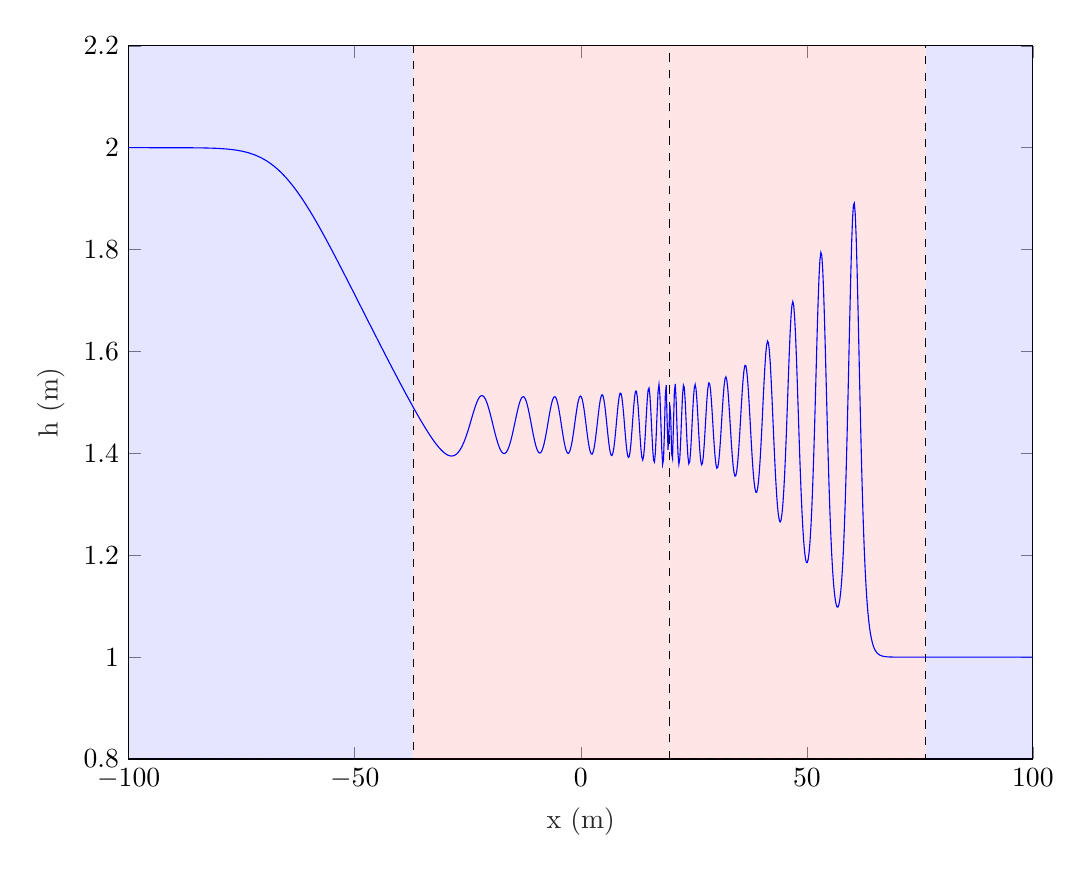
\begin{tikzpicture}

\begin{axis}[%
width=4.521in,
height=3.566in,
at={(0.758in,0.481in)},
scale only axis,
xmin=-100,
xmax=100,
xtick={-100,  -50,    0,   50,  100},
xlabel style={font=\color{white!15!black}},
xlabel={x (m)},
ymin=0.8,
ymax=2.2,
ytick={0.8,   1, 1.2, 1.4, 1.6, 1.8,   2, 2.2},
ylabel style={font=\color{white!15!black}},
ylabel={h (m)},
axis background/.style={fill=white}
]

\addplot[area legend, dashed, draw=black, fill=blue, fill opacity=0.1, forget plot]
table[row sep=crcr] {%
x	y\\
-100	0.8\\
-100	2.2\\
-37.0630892039997	2.2\\
-37.0630892039997	0.8\\
}--cycle;

\addplot[area legend, draw=none, fill=red, fill opacity=0.1, forget plot]
table[row sep=crcr] {%
x	y\\
-37.0630892039997	0.8\\
-37.0630892039997	2.2\\
19.5890566189392	2.2\\
19.5890566189392	0.8\\
}--cycle;

\addplot[area legend, draw=none, fill=green, fill opacity=0.1, forget plot]
table[row sep=crcr] {%
x	y\\
19.5890566189392	0.8\\
19.5890566189392	2.2\\
19.5890566189392	2.2\\
19.5890566189392	0.8\\
}--cycle;

\addplot[area legend, draw=none, fill=green, fill opacity=0.1, forget plot]
table[row sep=crcr] {%
x	y\\
19.5890566189392	0.8\\
19.5890566189392	2.2\\
19.5890566189392	2.2\\
19.5890566189392	0.8\\
}--cycle;

\addplot[area legend, dashed, draw=black, fill=red, fill opacity=0.1, forget plot]
table[row sep=crcr] {%
x	y\\
19.5890566189392	0.8\\
19.5890566189392	2.2\\
76.2412024418781	2.2\\
76.2412024418781	0.8\\
}--cycle;

\addplot[area legend, draw=none, fill=blue, fill opacity=0.1, forget plot]
table[row sep=crcr] {%
x	y\\
76.2412024418781	0.8\\
76.2412024418781	2.2\\
100	2.2\\
100	0.8\\
}--cycle;
\addplot [color=blue, forget plot]
  table[row sep=crcr]{%
-100.1200120012	2\\
-99.9199919991999	1.99999865169717\\
-99.7199719971997	1.99999862006113\\
-99.5199519951995	1.99999859617165\\
-99.3199319931993	1.9999985618233\\
-99.1199119911991	1.99999851675237\\
-98.9198919891989	1.99999846069871\\
-98.7198719871987	1.99999839328698\\
-98.5198519851985	1.99999831406379\\
-98.3198319831983	1.99999822249765\\
-98.1198119811981	1.99999811797599\\
-97.9197919791979	1.99999799980154\\
-97.7197719771977	1.99999786718834\\
-97.5197519751975	1.9999977192572\\
-97.3197319731973	1.99999755503068\\
-97.1197119711971	1.99999737342749\\
-96.9196919691969	1.99999717325636\\
-96.7196719671967	1.99999695320933\\
-96.5196519651965	1.99999671185434\\
-96.3196319631963	1.9999964476273\\
-96.1196119611961	1.99999615882331\\
-95.9195919591959	1.99999584358733\\
-95.7195719571957	1.99999549990392\\
-95.5195519551955	1.99999512558627\\
-95.3195319531953	1.99999471826435\\
-95.1195119511951	1.99999427537212\\
-94.9194919491949	1.99999379413386\\
-94.7194719471947	1.99999327154937\\
-94.5194519451945	1.9999927043782\\
-94.3194319431943	1.99999208912271\\
-94.1194119411941	1.99999142200987\\
-93.9193919391939	1.99999069897189\\
-93.7193719371937	1.9999899156254\\
-93.5193519351935	1.99998906724929\\
-93.3193319331933	1.99998814876095\\
-93.1193119311931	1.99998715469102\\
-92.9192919291929	1.99998607915632\\
-92.7192719271927	1.99998491583118\\
-92.5192519251925	1.99998365791669\\
-92.3192319231923	1.99998229810809\\
-92.1192119211921	1.99998082856004\\
-91.9191919191919	1.99997924084966\\
-91.7191719171917	1.99997752593725\\
-91.5191519151915	1.99997567412454\\
-91.3191319131913	1.99997367501042\\
-91.1191119111911	1.99997151744382\\
-90.9190919091909	1.99996918947392\\
-90.7190719071907	1.99996667829717\\
-90.5190519051905	1.99996397020131\\
-90.3190319031903	1.99996105050598\\
-90.1190119011901	1.99995790349991\\
-89.9189918991899	1.99995451237451\\
-89.7189718971897	1.9999508591536\\
-89.5189518951895	1.99994692461923\\
-89.3189318931893	1.99994268823328\\
-89.1189118911891	1.99993812805484\\
-88.9188918891889	1.99993322065299\\
-88.7188718871887	1.99992794101487\\
-88.5188518851885	1.99992226244897\\
-88.3188318831883	1.99991615648319\\
-88.1188118811881	1.99990959275776\\
-87.9187918791879	1.99990253891257\\
-87.7187718771877	1.99989496046894\\
-87.5187518751875	1.99988682070544\\
-87.3187318731873	1.99987808052768\\
-87.1187118711871	1.99986869833189\\
-86.9186918691869	1.99985862986204\\
-86.7186718671867	1.99984782806028\\
-86.5186518651865	1.9998362429107\\
-86.3186318631863	1.99982382127601\\
-86.1186118611861	1.9998105067272\\
-85.9185918591859	1.99979623936577\\
-85.7185718571857	1.99978095563872\\
-85.5185518551855	1.99976458814585\\
-85.3185318531853	1.99974706543944\\
-85.1185118511851	1.99972831181622\\
-84.9184918491849	1.99970824710148\\
-84.7184718471847	1.99968678642529\\
-84.5184518451845	1.99966383999083\\
-84.3184318431843	1.99963931283484\\
-84.1184118411841	1.99961310458021\\
-83.9183918391839	1.99958510918068\\
-83.7183718371837	1.9995552146579\\
-83.5183518351835	1.99952330283091\\
-83.3183318331833	1.99948924903823\\
-83.1183118311831	1.99945292185273\\
-82.9182918291829	1.99941418278965\\
-82.7182718271827	1.99937288600799\\
-82.5182518251825	1.9993288780058\\
-82.3182318231823	1.99928199730955\\
-82.1182118211821	1.99923207415834\\
-81.9181918191819	1.99917893018338\\
-81.7181718171817	1.99912237808332\\
-81.5181518151815	1.99906222129626\\
-81.3181318131813	1.99899825366915\\
-81.1181118111811	1.99893025912533\\
-80.9180918091809	1.99885801133135\\
-80.7180718071807	1.99878127336391\\
-80.5180518051805	1.998699797378\\
-80.3180318031803	1.99861332427765\\
-80.1180118011801	1.99852158339024\\
-79.9179917991799	1.99842429214596\\
-79.7179717971797	1.99832115576381\\
-79.5179517951795	1.9982118669456\\
-79.3179317931793	1.99809610557968\\
-79.1179117911791	1.99797353845606\\
-78.9178917891789	1.99784381899473\\
-78.7178717871787	1.99770658698907\\
-78.5178517851785	1.99756146836626\\
-78.3178317831783	1.9974080749669\\
-78.1178117811781	1.99724600434566\\
-77.9177917791779	1.99707483959551\\
-77.7177717771777	1.99689414919738\\
-77.5177517751775	1.99670348689784\\
-77.3177317731773	1.99650239161702\\
-77.1177117711771	1.99629038738899\\
-76.9176917691769	1.99606698333728\\
-76.7176717671767	1.9958316736876\\
-76.5176517651765	1.99558393782042\\
-76.3176317631763	1.9953232403655\\
-76.1176117611761	1.99504903134097\\
-75.9175917591759	1.99476074633892\\
-75.7175717571757	1.99445780676005\\
-75.5175517551755	1.9941396200991\\
-75.3175317531753	1.99380558028337\\
-75.1175117511751	1.99345506806602\\
-74.9174917491749	1.9930874514759\\
-74.7174717471747	1.99270208632552\\
-74.5174517451745	1.99229831677837\\
-74.3174317431743	1.99187547597684\\
-74.1174117411741	1.9914328867316\\
-73.9173917391739	1.99096986227309\\
-73.7173717371737	1.99048570706535\\
-73.5173517351735	1.98997971768247\\
-73.3173317331733	1.98945118374724\\
-73.1173117311731	1.9888993889314\\
-72.9172917291729	1.98832361201658\\
-72.7172717271727	1.9877231280147\\
-72.5172517251725	1.98709720934588\\
-72.3172317231723	1.98644512707204\\
-72.1172117211721	1.98576615218352\\
-71.9171917191719	1.98505955693594\\
-71.7171717171717	1.98432461623385\\
-71.5171517151715	1.98356060905772\\
-71.3171317131713	1.98276681992986\\
-71.1171117111711	1.981942540415\\
-70.9170917091709	1.98108707065064\\
-70.7170717071707	1.98019972090179\\
-70.5170517051705	1.97927981313468\\
-70.3170317031703	1.97832668260347\\
-70.1170117011701	1.97733967944382\\
-69.9169916991699	1.97631817026678\\
-69.7169716971697	1.97526153974644\\
-69.5169516951695	1.97416919219443\\
-69.3169316931693	1.97304055311423\\
-69.1169116911691	1.97187507072825\\
-68.9168916891689	1.97067221747046\\
-68.7168716871687	1.96943149143748\\
-68.5168516851685	1.9681524177909\\
-68.3168316831683	1.96683455010388\\
-68.1168116811681	1.9654774716452\\
-67.9167916791679	1.96408079659394\\
-67.7167716771677	1.96264417117856\\
-67.5167516751675	1.96116727473407\\
-67.3167316731673	1.95964982067179\\
-67.1167116711671	1.95809155735609\\
-66.9166916691669	1.95649226888339\\
-66.7166716671667	1.95485177575902\\
-66.5166516651665	1.95316993546795\\
-66.3166316631663	1.95144664293624\\
-66.1166116611661	1.94968183088037\\
-65.9165916591659	1.94787547004254\\
-65.7165716571657	1.94602756931029\\
-65.5165516551655	1.94413817571986\\
-65.3165316531653	1.94220737434304\\
-65.1165116511651	1.94023528805817\\
-64.9164916491649	1.93822207720634\\
-64.7164716471647	1.9361679391349\\
-64.5164516451645	1.93407310763059\\
-64.3164316431643	1.93193785224542\\
-64.1164116411641	1.92976247751928\\
-63.9163916391639	1.92754732210318\\
-63.7163716371637	1.92529275778827\\
-63.5163516351635	1.92299918844568\\
-63.3163316331633	1.92066704888319\\
-63.1163116311631	1.9182968036245\\
-62.9162916291629	1.91588894561798\\
-62.7162716271627	1.91344399488132\\
-62.5162516251625	1.91096249708936\\
-62.3162316231623	1.90844502211204\\
-62.1162116211621	1.90589216251003\\
-61.9161916191619	1.90330453199521\\
-61.7161716171617	1.90068276386358\\
-61.5161516151615	1.8980275094079\\
-61.3161316131613	1.89533943631725\\
-61.1161116111611	1.89261922707087\\
-60.9160916091609	1.88986757733314\\
-60.7160716071607	1.88708519435631\\
-60.5160516051605	1.88427279539777\\
-60.3160316031603	1.88143110615778\\
-60.1160116011601	1.87856085924356\\
-59.9159915991599	1.87566279266544\\
-59.7159715971597	1.8727376483698\\
-59.5159515951595	1.86978617081389\\
-59.3159315931593	1.86680910558659\\
-59.1159115911591	1.863807198079\\
-58.9158915891589	1.86078119220839\\
-58.7158715871587	1.85773182919834\\
-58.5158515851585	1.85465984641776\\
-58.3158315831583	1.85156597628086\\
-58.1158115811581	1.84845094520965\\
-57.9157915791579	1.84531547266049\\
-57.7157715771577	1.84216027021528\\
-57.5157515751575	1.83898604073804\\
-57.3157315731573	1.83579347759678\\
-57.1157115711571	1.83258326395062\\
-56.9156915691569	1.82935607210153\\
-56.7156715671567	1.82611256290978\\
-56.5156515651565	1.82285338527214\\
-56.3156315631563	1.81957917566128\\
-56.1156115611561	1.81629055772485\\
-55.9155915591559	1.81298814194248\\
-55.7155715571557	1.80967252533853\\
-55.5155515551555	1.80634429124868\\
-55.3155315531553	1.8030040091379\\
-55.1155115511551	1.79965223446753\\
-54.9154915491549	1.79628950860896\\
-54.7154715471547	1.79291635880141\\
-54.5154515451545	1.78953329815122\\
-54.3154315431543	1.78614082567013\\
-54.1154115411541	1.78273942634981\\
-53.9153915391539	1.7793295712703\\
-53.7153715371537	1.77591171773954\\
-53.5153515351535	1.77248630946165\\
-53.3153315331533	1.76905377673152\\
-53.1153115311531	1.76561453665316\\
-52.9152915291529	1.76216899337971\\
-52.7152715271527	1.75871753837261\\
-52.5152515251525	1.7552605506781\\
-52.3152315231523	1.75179839721875\\
-52.1152115211521	1.74833143309818\\
-51.9151915191519	1.7448600019171\\
-51.7151715171517	1.74138443609907\\
-51.5151515151515	1.73790505722406\\
-51.3151315131513	1.73442217636864\\
-51.1151115111511	1.73093609445123\\
-50.9150915091509	1.72744710258102\\
-50.7150715071507	1.72395548240968\\
-50.5150515051505	1.72046150648444\\
-50.3150315031503	1.71696543860191\\
-50.1150115011501	1.71346753416147\\
-49.9149914991499	1.70996804051774\\
-49.7149714971497	1.70646719733127\\
-49.5149514951495	1.70296523691698\\
-49.3149314931493	1.69946238458993\\
-49.1149114911491	1.69595885900783\\
-48.9148914891489	1.69245487251027\\
-48.7148714871487	1.68895063145412\\
-48.5148514851485	1.68544633654535\\
-48.3148314831483	1.68194218316681\\
-48.1148114811481	1.67843836170221\\
-47.9147914791479	1.67493505785636\\
-47.7147714771477	1.67143245297166\\
-47.5147514751475	1.66793072434123\\
-47.3147314731473	1.66443004551875\\
-47.1147114711471	1.66093058662555\\
-46.9146914691469	1.65743251465504\\
-46.7146714671467	1.65393599377524\\
-46.5146514651465	1.65044118562961\\
-46.3146314631463	1.64694824963689\\
-46.1146114611461	1.64345734329049\\
-45.9145914591459	1.63996862245812\\
-45.7145714571457	1.63648224168229\\
-45.5145514551455	1.63299835448253\\
-45.3145314531453	1.62951711366008\\
-45.1145114511451	1.626038671606\\
-44.9144914491449	1.62256318061357\\
-44.7144714471447	1.61909079319608\\
-44.5144514451445	1.61562166241103\\
-44.3144314431443	1.61215594219191\\
-44.1144114411441	1.60869378768881\\
-43.9143914391439	1.60523535561923\\
-43.7143714371437	1.60178080463039\\
-43.5143514351435	1.59833029567476\\
-43.3143314331433	1.59488399240021\\
-43.1143114311431	1.59144206155677\\
-42.9142914291429	1.58800467342169\\
-42.7142714271427	1.58457200224498\\
-42.5142514251425	1.58114422671749\\
-42.3142314231423	1.57772153046404\\
-42.1142114211421	1.57430410256401\\
-41.9141914191419	1.57089213810219\\
-41.7141714171417	1.56748583875287\\
-41.5141514151415	1.56408541340047\\
-41.3141314131413	1.56069107880003\\
-41.1141114111411	1.55730306028152\\
-40.9140914091409	1.55392159250199\\
-40.7140714071407	1.55054692025009\\
-40.5140514051405	1.54717929930772\\
-40.3140314031403	1.54381899737428\\
-40.1140114011401	1.54046629505903\\
-39.9139913991399	1.53712148694809\\
-39.7139713971397	1.53378488275269\\
-39.5139513951395	1.53045680854622\\
-39.3139313931393	1.5271376080982\\
-39.1139113911391	1.52382764431403\\
-38.9138913891389	1.52052730079001\\
-38.7138713871387	1.51723698349445\\
-38.5138513851385	1.51395712258605\\
-38.3138313831383	1.51068817438234\\
-38.1138113811381	1.50743062349163\\
-37.9137913791379	1.50418498512351\\
-37.7137713771377	1.50095180759407\\
-37.5137513751375	1.49773167504362\\
-37.3137313731373	1.49452521038607\\
-37.1137113711371	1.49133307851103\\
-36.9136913691369	1.48815598976148\\
-36.7136713671367	1.48499470371173\\
-36.5136513651365	1.48185003327261\\
-36.3136313631363	1.47872284915312\\
-36.1136113611361	1.47561408471003\\
-35.9135913591359	1.47252474121973\\
-35.7135713571357	1.46945589360891\\
-35.5135513551355	1.46640869668384\\
-35.3135313531353	1.46338439190073\\
-35.1135113511351	1.46038431472256\\
-34.9134913491349	1.45740990261084\\
-34.7134713471347	1.45446270370364\\
-34.5134513451345	1.45154438623418\\
-34.3134313431343	1.44865674874674\\
-34.1134113411341	1.44580173116915\\
-33.9133913391339	1.44298142680273\\
-33.7133713371337	1.44019809529197\\
-33.5133513351335	1.43745417663627\\
-33.3133313331333	1.43475230630519\\
-33.1133113311331	1.43209533151601\\
-32.9132913291329	1.42948632872788\\
-32.7132713271327	1.42692862239964\\
-32.5132513251325	1.42442580504773\\
-32.3132313231323	1.42198175862636\\
-32.1132113211321	1.41960067723232\\
-31.9131913191319	1.41728709111121\\
-31.7131713171317	1.41504589190858\\
-31.5131513151315	1.41288235906712\\
-31.3131313131313	1.41080218721785\\
-31.1131113111311	1.40881151434681\\
-30.9130913091309	1.40691695043699\\
-30.7130713071307	1.40512560618541\\
-30.5130513051305	1.40344512127357\\
-30.3130313031303	1.40188369152438\\
-30.1130113011301	1.40045009410413\\
-29.9129912991299	1.39915370972324\\
-29.7129712971297	1.39800454054832\\
-29.5129512951295	1.39701322225919\\
-29.3129312931293	1.39619102836406\\
-29.1129112911291	1.39554986452316\\
-28.9128912891289	1.39510225022613\\
-28.7128712871287	1.39486128424988\\
-28.5128512851285	1.39484060359914\\
-28.3128312831283	1.39505425448599\\
-28.1128112811281	1.39551668355926\\
-27.9127912791279	1.39624250916747\\
-27.7127712771277	1.39724638878018\\
-27.5127512751275	1.39854279181106\\
-27.3127312731273	1.40014572403964\\
-27.1127112711271	1.40206840598566\\
-26.9126912691269	1.40432288327962\\
-26.7126712671267	1.40691956941307\\
-26.5126512651265	1.40986673129623\\
-26.3126312631263	1.41316988834813\\
-26.1126112611261	1.41683116374297\\
-25.9125912591259	1.42084856078493\\
-25.7125712571257	1.42521519978584\\
-25.5125512551255	1.42991852437865\\
-25.3125312531253	1.43493949737206\\
-25.1125112511251	1.44025183608913\\
-24.9124912491249	1.4458213052852\\
-24.7124712471247	1.45160514240918\\
-24.5124512451245	1.45755164956524\\
-24.3124312431243	1.4636000289932\\
-24.1124112411241	1.46968051824684\\
-23.9123912391239	1.47571488158572\\
-23.7123712371237	1.4816173210023\\
-23.5123512351235	1.48729582231595\\
-23.3123312331233	1.49265397526132\\
-23.1123112311231	1.49759322520112\\
-22.9122912291229	1.50201553445992\\
-22.7122712271227	1.50582634652674\\
-22.5122512251225	1.50893775078924\\
-22.3122312231223	1.51127168665903\\
-22.1122112211221	1.51276302303065\\
-21.9121912191219	1.51336439258599\\
-21.7121712171217	1.51303813339246\\
-21.5121512151215	1.51177869803604\\
-21.3121312131213	1.50959275093816\\
-21.1121112111211	1.50650974713821\\
-20.9120912091209	1.50257907337884\\
-20.7120712071207	1.49786861420747\\
-20.5120512051205	1.49246260476352\\
-20.3120312031203	1.48645899222348\\
-20.1120112011201	1.47996644421292\\
-19.9119911991199	1.47310120413117\\
-19.7119711971197	1.46598396498907\\
-19.5119511951195	1.45873691666312\\
-19.3119311931193	1.4514810982839\\
-19.1119111911191	1.44433413879326\\
-18.9118911891189	1.43740843815247\\
-18.7118711871187	1.43080979949613\\
-18.5118511851185	1.42463648542134\\
-18.3118311831183	1.41897864990803\\
-18.1118111811181	1.41391807735053\\
-17.9117911791179	1.40952813324692\\
-17.7117711771177	1.40587384594415\\
-17.5117511751175	1.40301201767043\\
-17.3117311731173	1.40099127828551\\
-17.1117111711171	1.39985199372164\\
-16.9116911691169	1.3996264835979\\
-16.7116711671167	1.40033584997702\\
-16.5116511651165	1.40199422889866\\
-16.3116311631163	1.40460242656371\\
-16.1116111611161	1.40814890342068\\
-15.9115911591159	1.41260740725068\\
-15.7115711571157	1.4179348910106\\
-15.5115511551155	1.42406934761427\\
-15.3115311531153	1.43092772727379\\
-15.1115111511151	1.43840415615839\\
-14.9114911491149	1.44636874185377\\
-14.7114711471147	1.45466725444766\\
-14.5114511451145	1.46312200638583\\
-14.3114311431143	1.47153421488221\\
-14.1114111411141	1.47968809033353\\
-13.9113911391139	1.48735674021362\\
-13.7113711371137	1.49430985606244\\
-13.5113511351135	1.50032293312666\\
-13.3113311331133	1.50518755830568\\
-13.1113111311131	1.50872210491607\\
-12.9112911291129	1.51078202029255\\
-12.7112711271127	1.51126670758975\\
-12.5112511251125	1.51013694100651\\
-12.3112311231123	1.50739793513333\\
-12.1112111211121	1.50312111776661\\
-11.9111911191119	1.49743116566056\\
-11.7111711171117	1.49050253389894\\
-11.5111511151115	1.48255135264657\\
-11.3111311131113	1.47382555138004\\
-11.1111111111111	1.46459413306526\\
-10.9110911091109	1.45513640694312\\
-10.7110711071107	1.44573195980237\\
-10.5110511051105	1.43665193292781\\
-10.3110311031103	1.4281518461226\\
-10.1110111011101	1.42046613676688\\
-9.91099109910991	1.41380421617841\\
-9.71097109710971	1.40834779417533\\
-9.5109510951095	1.40424905868997\\
-9.3109310931093	1.40162931583936\\
-9.1109110911091	1.40057409398118\\
-8.9108910891089	1.40114915342226\\
-8.7108710871087	1.40336273145064\\
-8.51085108510851	1.40719810255538\\
-8.31083108310831	1.41259213547941\\
-8.11081108110811	1.41943489269837\\
-7.91079107910791	1.42756575979107\\
-7.71077107710771	1.43677045821344\\
-7.51075107510751	1.44677983165477\\
-7.31073107310731	1.45727148279636\\
-7.1107110711071	1.46787528790258\\
-6.9106910691069	1.47818367616966\\
-6.7106710671067	1.48776711243055\\
-6.5106510651065	1.49619464303506\\
-6.3106310631063	1.50305849771428\\
-6.11061106110611	1.50800096756325\\
-5.91059105910591	1.51074096886103\\
-5.71057105710571	1.51109676804922\\
-5.51055105510551	1.50900598605086\\
-5.31053105310531	1.50452886608788\\
-5.11051105110511	1.49785239375764\\
-4.91049104910491	1.48927706632858\\
-4.7104710471047	1.4791983745587\\
-4.5104510451045	1.46808195408478\\
-4.3104310431043	1.4564358235213\\
-4.1104110411041	1.4447826696534\\
-3.9103910391039	1.43363454375183\\
-3.71037103710371	1.42347159882956\\
-3.51035103510351	1.41472543817286\\
-3.31033103310331	1.40776687590508\\
-3.11031103110311	1.40289716490152\\
-2.91029102910291	1.40034145765665\\
-2.71027102710271	1.40024352361\\
-2.51025102510251	1.40265847543276\\
-2.3102310231023	1.40754876430179\\
-2.1102110211021	1.41477438406529\\
-1.9101910191019	1.42408685515911\\
-1.7101710171017	1.43512360755983\\
-1.5101510151015	1.44740721644568\\
-1.31013101310131	1.46035212243768\\
-1.11011101110111	1.47328195456129\\
-0.91009100910091	1.48545988837435\\
-0.710071007100709	1.49613246739663\\
-0.510051005100507	1.50458501127726\\
-0.310031003100306	1.51020370652436\\
-0.110011001100105	1.51254722890683\\
0.0900090009000962	1.51134541190087\\
0.290029002900297	1.50663747984908\\
0.490049004900499	1.4986744508104\\
0.6900690069007	1.48795391018062\\
0.890089008900901	1.47516787145825\\
1.09010901090109	1.46114468111199\\
1.29012901290129	1.44678337478267\\
1.49014901490149	1.43298917755149\\
1.69016901690169	1.42061688944581\\
1.89018901890189	1.41042558964212\\
2.09020902090209	1.40304500140681\\
2.2902290229023	1.39895124589014\\
2.4902490249025	1.39844894558833\\
2.6902690269027	1.40165342808507\\
2.8902890289029	1.40847807495345\\
3.0903090309031	1.41861596669603\\
3.2903290329033	1.43152892235542\\
3.4903490349035	1.44644436631367\\
3.69036903690369	1.462370262952\\
3.89038903890389	1.47813688268393\\
4.09040904090409	1.49247203743592\\
4.29042904290429	1.50411041081704\\
4.49044904490449	1.5119284375236\\
4.6904690469047	1.51510408332125\\
4.8904890489049	1.5131510816679\\
5.0905090509051	1.50617629403347\\
5.2905290529053	1.49471452375569\\
5.4905490549055	1.47976403316601\\
5.6905690569057	1.46265703962015\\
5.8905890589059	1.44491444942119\\
6.09060906090609	1.42809390508066\\
6.29062906290629	1.41365358579359\\
6.49064906490649	1.40284434146034\\
6.69066906690669	1.39663086031406\\
6.89068906890689	1.39563856244427\\
7.0907090709071	1.40009376748239\\
7.2907290729073	1.40981450475234\\
7.4907490749075	1.42414623370387\\
7.6907690769077	1.44195722540413\\
7.8907890789079	1.46165290469053\\
8.0908090809081	1.48125656756959\\
8.2908290829083	1.4985767066234\\
8.49084908490849	1.51146535381617\\
8.69086908690869	1.518137981006\\
8.89088908890889	1.51750468506901\\
9.09090909090909	1.5093960516923\\
9.29092909290929	1.49466175396188\\
9.4909490949095	1.4750631997389\\
9.6909690969097	1.453012538522\\
9.8909890989099	1.43122282843778\\
10.0910091009101	1.41235316596912\\
10.2910291029103	1.39871067947214\\
10.4910491049105	1.39203229590858\\
10.6910691069107	1.39332436968945\\
10.8910891089109	1.40275382432918\\
11.0911091109111	1.41954005454037\\
11.2911291129113	1.44188746625149\\
11.4911491149115	1.46700404537911\\
11.6911691169117	1.49129386885725\\
11.8911891189119	1.51080319531467\\
12.0912091209121	1.52192270127121\\
12.2912291229123	1.52222073118981\\
12.4912491249125	1.51113988579522\\
12.6912691269127	1.49030129069562\\
12.8912891289129	1.46324305930165\\
13.0913091309131	1.43470647419109\\
13.2913291329133	1.40971208690484\\
13.4913491349135	1.39270338438594\\
13.6913691369137	1.38692257474096\\
13.8913891389139	1.39384659810138\\
14.0914091409141	1.41305577727099\\
14.2914291429143	1.44173825026312\\
14.4914491449145	1.47473127385398\\
14.6914691469147	1.50496778625546\\
14.8914891489149	1.52481466326601\\
15.0915091509151	1.52823752793579\\
15.2915291529153	1.51317592154669\\
15.4915491549155	1.4827567161734\\
15.6915691569157	1.44476374658805\\
15.8915891589159	1.4093769220162\\
16.0916091609161	1.38637999862919\\
16.2916291629163	1.38283519449485\\
16.4916491649165	1.4012346867153\\
16.6916691669167	1.4383190267513\\
16.8916891689169	1.48394639371489\\
17.0917091709171	1.52198511946431\\
17.2917291729173	1.53523467467046\\
17.4917491749175	1.5146471614756\\
17.6917691769177	1.46623289917901\\
17.8917891789179	1.41168314660581\\
18.0918091809181	1.37828431423467\\
18.2918291829183	1.38750512887909\\
18.4918491849185	1.44178396140033\\
18.6918691869187	1.51358274539563\\
18.8918891889189	1.5337748393366\\
19.0919091909191	1.46368135191428\\
19.2919291929193	1.40694364490548\\
19.4919491949195	1.44096466782303\\
19.6919691969197	1.49587624157044\\
19.8919891989199	1.47007466392253\\
20.0920092009201	1.39941664509229\\
20.2920292029203	1.39009997674821\\
20.4920492049205	1.45544980215266\\
20.6920692069207	1.5205354399639\\
20.8920892089209	1.53633184834134\\
21.0921092109211	1.502451381342\\
21.2921292129213	1.44684343522972\\
21.4921492149215	1.39938326366126\\
21.6921692169217	1.37880081811537\\
21.8921892189219	1.38944457773131\\
22.0922092209221	1.42510706875513\\
22.2922292229223	1.47179511504615\\
22.4922492249225	1.51271515670663\\
22.6922692269227	1.53385770953271\\
22.8922892289229	1.52918933315166\\
23.0923092309231	1.50207613091681\\
23.2923292329233	1.46269939342862\\
23.4923492349235	1.42313562932947\\
23.6923692369237	1.39341070792244\\
23.8923892389239	1.37965931985049\\
24.0924092409241	1.38381663893629\\
24.2924292429243	1.4042472010669\\
24.4924492449245	1.43619914492564\\
24.6924692469247	1.47270835304523\\
24.8924892489249	1.50580258914454\\
25.0925092509251	1.52822241096371\\
25.2925292529253	1.53525122380827\\
25.4925492549255	1.5258371579067\\
25.6925692569257	1.50275663070397\\
25.8925892589259	1.47136705370361\\
26.0926092609261	1.43802562992508\\
26.2926292629263	1.4086028911827\\
26.4926492649265	1.38756825670306\\
26.6926692669267	1.3776478304452\\
26.8926892689269	1.37981337222243\\
27.0927092709271	1.39347477902461\\
27.2927292729273	1.41659112652786\\
27.4927492749275	1.44588819459874\\
27.6927692769277	1.47714777954457\\
27.8927892789279	1.50570704312435\\
28.0928092809281	1.52717046600023\\
28.2928292829283	1.53821092627401\\
28.4928492849285	1.53723031052929\\
28.6928692869287	1.52464361662506\\
28.8928892889289	1.50267543945563\\
29.0929092909291	1.47479095065918\\
29.2929292929293	1.44494282733099\\
29.4929492949295	1.41690307224138\\
29.6929692969297	1.39380648773358\\
29.8929892989299	1.37793109016896\\
30.0930093009301	1.3706581479008\\
30.2930293029303	1.3724990754297\\
30.4930493049305	1.38319793039816\\
30.6930693069307	1.4017362982918\\
30.8930893089309	1.42639207299475\\
31.0931093109311	1.45479182760144\\
31.2931293129313	1.48404135424999\\
31.4931493149315	1.5109699948137\\
31.6931693169317	1.53249359680183\\
31.8931893189319	1.54605012790034\\
32.0932093209321	1.55002912351647\\
32.2932293229323	1.54394024667153\\
32.4932493249325	1.528659682034\\
32.6932693269327	1.50604141029318\\
32.8932893289329	1.47865505404726\\
33.0933093309331	1.44934673975137\\
33.2933293329333	1.42086412604813\\
33.4933493349335	1.39559230541144\\
33.6933693369337	1.3754157325042\\
33.8933893389339	1.36168276269192\\
34.0934093409341	1.35523263508704\\
34.2934293429343	1.35643467865645\\
34.4934493449345	1.36523824305697\\
34.6934693469347	1.38116696782372\\
34.8934893489349	1.40331467641184\\
35.0935093509351	1.4303197071544\\
35.2935293529353	1.46035953562129\\
35.4935493549355	1.49119538217899\\
35.6935693569357	1.52029667787503\\
35.8935893589359	1.54505819864431\\
36.0936093609361	1.56309470997258\\
36.2936293629363	1.57256312212781\\
36.4936493649365	1.57243805168507\\
36.6936693669367	1.56267992827946\\
36.8936893689369	1.54420633698854\\
37.0937093709371	1.51874815224132\\
37.2937293729373	1.48855721125747\\
37.4937493749375	1.45609339060288\\
37.6937693769377	1.42374310999441\\
37.8937893789379	1.39361828283324\\
38.0938093809381	1.36744933500573\\
38.2938293829383	1.3465599918653\\
38.4938493849385	1.33189676221499\\
38.6938693869387	1.32408339996751\\
38.8938893889389	1.32347558894689\\
39.0939093909391	1.33019051217073\\
39.2939293929393	1.34412286618221\\
39.4939493949395	1.36490711895966\\
39.6939693969397	1.39186873342914\\
39.8939893989399	1.4239534810343\\
40.0940094009401	1.45966440046109\\
40.2940294029403	1.49703472905298\\
40.4940494049405	1.53367005382754\\
40.6940694069407	1.56688676051249\\
40.8940894089409	1.59395517832631\\
41.0941094109411	1.61242394475984\\
41.2941294129413	1.62045423712026\\
41.4941494149415	1.61717151640068\\
41.6941694169417	1.60268568289968\\
41.8941894189419	1.57819338603396\\
42.0942094209421	1.54570449939172\\
42.2942294229423	1.50774040772907\\
42.4942494249425	1.46698686723372\\
42.6942694269427	1.4259936536974\\
42.8942894289429	1.38696850611047\\
43.0943094309431	1.35167792862277\\
43.2943294329433	1.32143986125114\\
43.4943494349435	1.29717888928858\\
43.6943694369437	1.27951264894151\\
43.8943894389439	1.26884307632448\\
44.0944094409441	1.26543399824925\\
44.2944294429443	1.26946226807241\\
44.4944494449445	1.28103925154168\\
44.6944694469447	1.30019158451293\\
44.8944894489449	1.32680790616156\\
45.0945094509451	1.36054749475644\\
45.2945294529453	1.40072013209877\\
45.4945494549455	1.44615300346376\\
45.6945694569457	1.49507386375529\\
45.8945894589459	1.54505169918902\\
46.0946094609461	1.59304428552698\\
46.2946294629463	1.63559356842071\\
46.4946494649465	1.66918014892549\\
46.6946694669467	1.69069737373777\\
46.8946894689469	1.69793072329836\\
47.0947094709471	1.69003733221296\\
47.2947294729473	1.66753358385509\\
47.4947494749475	1.63236421882112\\
47.6947694769477	1.58745512800156\\
47.8947894789479	1.53624300436785\\
48.0948094809481	1.48218373020541\\
48.2948294829483	1.42836540970973\\
48.4948494849485	1.37727852143492\\
48.6948694869487	1.33074183582916\\
48.8948894889489	1.28994757168115\\
49.0949094909491	1.25557756084616\\
49.2949294929493	1.22794695243529\\
49.4949494949495	1.20714498294591\\
49.6949694969497	1.19315558276438\\
49.8949894989499	1.18594966847847\\
50.0950095009501	1.18555132165929\\
50.2950295029503	1.1920679174115\\
50.4950495049505	1.20570645559714\\
50.6950695069507	1.2267448084908\\
50.8950895089509	1.25548088873891\\
51.0951095109511	1.29213959074597\\
51.2951295129513	1.33673790659554\\
51.4951495149515	1.38890855950493\\
51.6951695169517	1.4476941466134\\
51.8951895189519	1.51134267267737\\
52.0952095209521	1.57715888828604\\
52.2952295229523	1.64148608259331\\
52.4952495249525	1.69989535614445\\
52.6952695269527	1.74762688093506\\
52.8952895289529	1.78025338898373\\
53.0953095309531	1.7944142163797\\
53.2953295329533	1.78858534826948\\
53.4953495349535	1.76315869174724\\
53.6953695369537	1.72059994352533\\
53.8953895389539	1.66481138143829\\
54.0954095409541	1.60043307719713\\
54.2954295429543	1.53210169921358\\
54.4954495449545	1.46387489040417\\
54.6954695469547	1.39890366780273\\
54.8954895489549	1.33934401215998\\
55.0955095509551	1.28644315249128\\
55.2955295529553	1.24072078257889\\
55.4955495549555	1.20217909512712\\
55.6955695569557	1.1704983750572\\
55.8955895589559	1.14519660106222\\
56.0956095609561	1.12574943568353\\
56.2956295629563	1.11167452353852\\
56.4956495649565	1.10258570844148\\
56.6956695669567	1.09822848850436\\
56.8956895689569	1.09850065082908\\
57.0957095709571	1.10346322148474\\
57.2957295729573	1.11334537743305\\
57.4957495749575	1.1285402370583\\
57.6957695769577	1.14959142265489\\
57.8957895789579	1.17716299064474\\
58.0958095809581	1.21198339487683\\
58.2958295829583	1.25475569896509\\
58.4958495849585	1.30601764831471\\
58.6958695869587	1.36594581620179\\
58.8958895889589	1.43410647339838\\
59.0959095909591	1.50917235609832\\
59.2959295929593	1.58866024038636\\
59.4959495949595	1.66877993508323\\
59.6959695969597	1.74450879691196\\
59.8959895989599	1.80999323457044\\
60.0960096009601	1.85930415787525\\
60.2960296029603	1.88743889021119\\
60.4960496049605	1.89136381846522\\
60.6960696069607	1.87045481002682\\
60.8960896089609	1.82707974386869\\
61.0961096109611	1.76562361682183\\
61.2961296129613	1.69180141692104\\
61.4961496149615	1.61157543061973\\
61.6961696169617	1.53029305865333\\
61.8961896189619	1.45215873903127\\
62.0962096209621	1.38005420310431\\
62.2962296229623	1.31562338730572\\
62.4962496249625	1.25950582182146\\
62.6962696269627	1.21161735455752\\
62.8962896289629	1.17141197495346\\
63.0963096309631	1.13809276480282\\
63.2963296329633	1.11076441176257\\
63.4963496349635	1.08853325538341\\
63.6963696369637	1.07056618621158\\
63.8963896389639	1.05612021016169\\
64.0964096409641	1.04455271825934\\
64.2964296429643	1.03532006688759\\
64.4964496449645	1.02796978273737\\
64.6964696469647	1.02212986640824\\
64.8964896489649	1.01749732234115\\
65.0965096509651	1.01382712125699\\
65.2965296529653	1.01092220416546\\
65.4965496549655	1.00862476993423\\
65.6965696569657	1.0068088758649\\
65.8965896589659	1.0053742674241\\
66.0966096609661	1.00424130103718\\
66.2966296629663	1.00334680742566\\
66.4966496649665	1.00264074627248\\
66.6966696669667	1.00208351613959\\
66.8966896689669	1.00164380068742\\
67.0967096709671	1.00129685005928\\
67.2967296729673	1.00102311307171\\
67.4967496749675	1.00080715080393\\
67.6967696769677	1.00063677505294\\
67.8967896789679	1.00050236595091\\
68.0968096809681	1.00039633200526\\
68.2968296829683	1.00031268315557\\
68.4968496849685	1.00024669338932\\
68.6968696869687	1.00019463425086\\
68.8968896889689	1.00015356442146\\
69.0969096909691	1.00012116361816\\
69.2969296929693	1.00009560150447\\
69.4969496949695	1.00007543424962\\
69.6969696969697	1.00005952291475\\
69.8969896989699	1.00004696906624\\
70.0970097009701	1.00003706398333\\
70.2970297029703	1.00002924859151\\
70.4970497049705	1.00002308185796\\
70.6970697069707	1.00001821586219\\
70.8970897089709	1.00001437613232\\
71.0971097109711	1.00001134613479\\
71.2971297129713	1.00000895504016\\
71.4971497149715	1.00000706807298\\
71.6971697169717	1.00000557889976\\
71.8971897189719	1.00000440362458\\
72.0972097209721	1.00000347605276\\
72.2972297229723	1.00000274395457\\
72.4972497249725	1.00000216611793\\
72.6972697269727	1.00000171002332\\
72.8972897289729	1.00000135000961\\
73.0973097309731	1.00000106582696\\
73.2973297329733	1.00000084149528\\
73.4973497349735	1.00000066440353\\
73.6973697369737	1.00000052459913\\
73.8973897389739	1.00000041422728\\
74.0974097409741	1.00000032708863\\
74.2974297429743	1.0000002582902\\
74.4974497449745	1.00000020396997\\
74.6974697469747	1.00000016107958\\
74.8974897489749	1.00000012721279\\
75.0975097509751	1.00000010047018\\
75.2975297529753	1.00000007935236\\
75.4975497549755	1.00000006267565\\
75.6975697569757	1.00000004950559\\
75.8975897589759	1.00000003910445\\
76.0976097609761	1.00000003088976\\
76.2976297629763	1.00000002440168\\
76.4976497649765	1.00000001927709\\
76.6976697669767	1.0000000152293\\
76.8976897689769	1.00000001203193\\
77.0977097709771	1.00000000950621\\
77.2977297729773	1.00000000751098\\
77.4977497749775	1.00000000593475\\
77.6977697769777	1.00000000468949\\
77.8977897789779	1.00000000370566\\
78.0978097809781	1.00000000292835\\
78.2978297829783	1.00000000231418\\
78.4978497849785	1.00000000182889\\
78.6978697869787	1.00000000144543\\
78.8978897889789	1.0000000011424\\
79.0979097909791	1.00000000090295\\
79.2979297929793	1.00000000071371\\
79.4979497949795	1.00000000056415\\
79.6979697969797	1.00000000044595\\
79.8979897989799	1.00000000035253\\
80.0980098009801	1.00000000027869\\
80.2980298029803	1.00000000022032\\
80.4980498049805	1.00000000017419\\
80.6980698069807	1.00000000013772\\
80.8980898089809	1.00000000010888\\
81.0981098109811	1.00000000008609\\
81.2981298129813	1.00000000006807\\
81.4981498149815	1.00000000005383\\
81.6981698169817	1.00000000004256\\
81.8981898189819	1.00000000003366\\
82.0982098209821	1.00000000002662\\
82.2982298229823	1.00000000002105\\
82.4982498249825	1.00000000001664\\
82.6982698269827	1.00000000001316\\
82.8982898289829	1.00000000001041\\
83.0983098309831	1.00000000000823\\
83.2983298329833	1.00000000000651\\
83.4983498349835	1.00000000000515\\
83.6983698369837	1.00000000000407\\
83.8983898389839	1.00000000000322\\
84.0984098409841	1.00000000000254\\
84.2984298429843	1.00000000000201\\
84.4984498449845	1.00000000000158\\
84.6984698469847	1.00000000000125\\
84.8984898489849	1.00000000000099\\
85.0985098509851	1.00000000000078\\
85.2985298529853	1.00000000000061\\
85.4985498549855	1.00000000000048\\
85.6985698569857	1.00000000000038\\
85.8985898589859	1.0000000000003\\
86.0986098609861	1.00000000000023\\
86.2986298629863	1.00000000000018\\
86.4986498649865	1.00000000000014\\
86.6986698669867	1.00000000000011\\
86.8986898689869	1.00000000000008\\
87.0987098709871	1.00000000000006\\
87.2987298729873	1.00000000000005\\
87.4987498749875	1.00000000000004\\
87.6987698769877	1.00000000000003\\
87.8987898789879	1.00000000000002\\
88.0988098809881	1.00000000000001\\
88.2988298829883	1.00000000000001\\
88.4988498849885	1\\
88.6988698869887	1\\
88.8988898889889	1\\
89.0989098909891	1\\
89.2989298929893	1\\
89.4989498949895	1\\
89.6989698969897	1\\
89.8989898989899	1\\
90.0990099009901	1\\
90.2990299029903	1\\
90.4990499049905	1\\
90.6990699069907	1\\
90.8990899089909	1\\
91.0991099109911	1\\
91.2991299129913	1\\
91.4991499149915	1\\
91.6991699169917	1\\
91.8991899189919	1\\
92.0992099209921	1\\
92.2992299229923	1\\
92.4992499249925	1\\
92.6992699269927	1\\
92.8992899289929	1\\
93.0993099309931	1\\
93.2993299329933	1\\
93.4993499349935	1\\
93.6993699369937	1\\
93.8993899389939	1\\
94.0994099409941	1\\
94.2994299429943	1\\
94.4994499449945	1\\
94.6994699469947	1\\
94.8994899489949	1\\
95.0995099509951	1\\
95.2995299529953	1\\
95.4995499549955	1\\
95.6995699569957	1\\
95.8995899589959	1\\
96.0996099609961	1\\
96.2996299629963	1\\
96.4996499649965	1\\
96.6996699669967	1\\
96.8996899689969	1\\
97.0997099709971	1\\
97.2997299729973	1\\
97.4997499749975	1\\
97.6997699769977	1\\
97.8997899789979	1\\
98.0998099809981	1\\
98.2998299829983	1\\
98.4998499849985	1\\
98.6998699869987	1\\
98.8998899889989	1\\
99.0999099909991	1\\
99.2999299929993	1\\
99.4999499949995	1\\
99.6999699969997	1\\
99.8999899989999	1\\
100.100010001	1\\
};
\end{axis}
\end{tikzpicture}%
		\caption{$h$}
	\end{subfigure}
	\begin{subfigure}{0.49\textwidth}
		\centering
		% This file was created by matlab2tikz.
%
%The latest updates can be retrieved from
%  http://www.mathworks.com/matlabcentral/fileexchange/22022-matlab2tikz-matlab2tikz
%where you can also make suggestions and rate matlab2tikz.
%
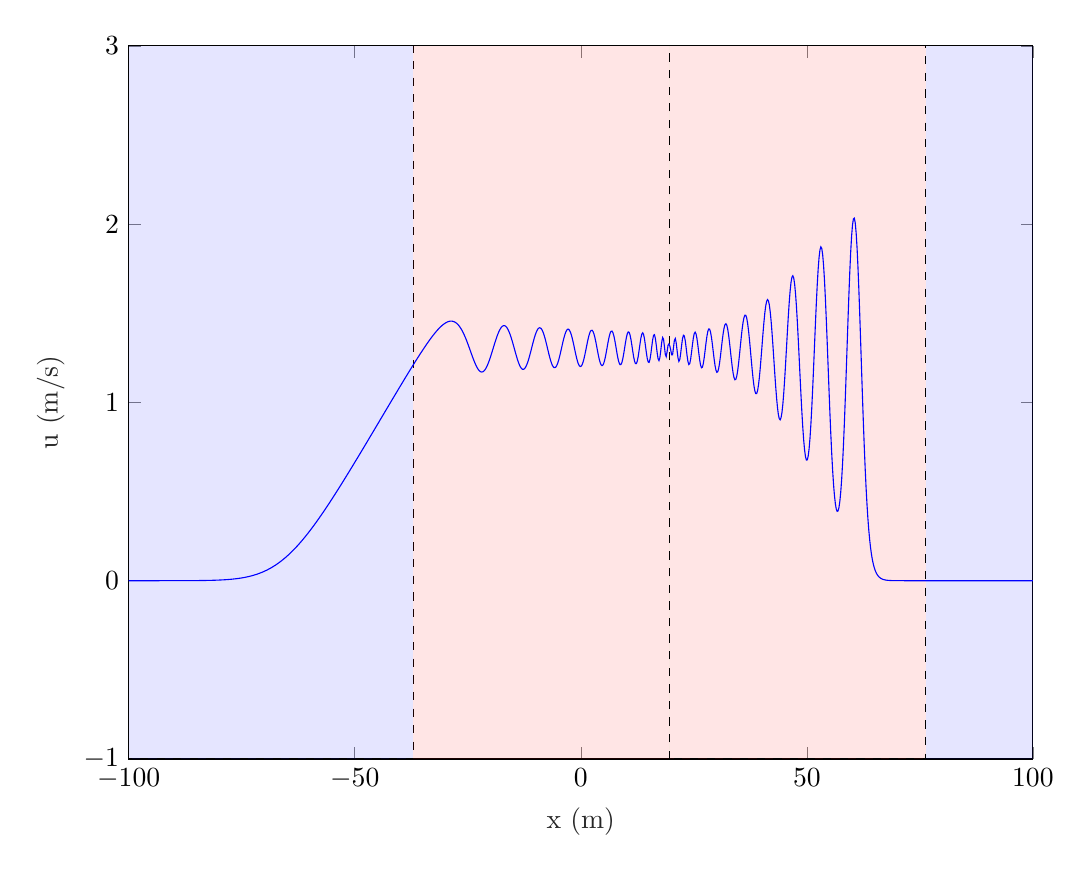
\begin{tikzpicture}

\begin{axis}[%
width=4.521in,
height=3.566in,
at={(0.758in,0.481in)},
scale only axis,
xmin=-100,
xmax=100,
xtick={-100,  -50,    0,   50,  100},
xlabel style={font=\color{white!15!black}},
xlabel={x (m)},
ymin=-1,
ymax=3,
ytick={-1,  0,  1,  2,  3},
ylabel style={font=\color{white!15!black}},
ylabel={u (m/s)},
axis background/.style={fill=white}
]

\addplot[area legend, dashed, draw=black, fill=blue, fill opacity=0.1, forget plot]
table[row sep=crcr] {%
x	y\\
-100	-1\\
-100	3\\
-37.0630892039997	3\\
-37.0630892039997	-1\\
}--cycle;

\addplot[area legend, draw=none, fill=red, fill opacity=0.1, forget plot]
table[row sep=crcr] {%
x	y\\
-37.0630892039997	-1\\
-37.0630892039997	3\\
19.5890566189392	3\\
19.5890566189392	-1\\
}--cycle;

\addplot[area legend, draw=none, fill=green, fill opacity=0.1, forget plot]
table[row sep=crcr] {%
x	y\\
19.5890566189392	-1\\
19.5890566189392	3\\
19.5890566189392	3\\
19.5890566189392	-1\\
}--cycle;

\addplot[area legend, draw=none, fill=green, fill opacity=0.1, forget plot]
table[row sep=crcr] {%
x	y\\
19.5890566189392	-1\\
19.5890566189392	3\\
19.5890566189392	3\\
19.5890566189392	-1\\
}--cycle;

\addplot[area legend, dashed, draw=black, fill=red, fill opacity=0.1, forget plot]
table[row sep=crcr] {%
x	y\\
19.5890566189392	-1\\
19.5890566189392	3\\
76.2412024418781	3\\
76.2412024418781	-1\\
}--cycle;

\addplot[area legend, draw=none, fill=blue, fill opacity=0.1, forget plot]
table[row sep=crcr] {%
x	y\\
76.2412024418781	-1\\
76.2412024418781	3\\
100	3\\
100	-1\\
}--cycle;
\addplot [color=blue, forget plot]
  table[row sep=crcr]{%
-100.1200120012	0\\
-99.9199919991999	2.39270327599359e-07\\
-99.7199719971997	5.52980030761066e-07\\
-99.5199519951995	8.59311040889484e-07\\
-99.3199319931993	1.17165035094555e-06\\
-99.1199119911991	1.49223414517356e-06\\
-98.9198919891989	1.82328146723547e-06\\
-98.7198719871987	2.16708110768666e-06\\
-98.5198519851985	2.52600094004348e-06\\
-98.3198319831983	2.90250212945175e-06\\
-98.1198119811981	3.29915397174849e-06\\
-97.9197919791979	3.71864928934013e-06\\
-97.7197719771977	4.16382046106673e-06\\
-97.5197519751975	4.63765615911085e-06\\
-97.3197319731973	5.14331887973674e-06\\
-97.1197119711971	5.68416334770379e-06\\
-96.9196919691969	6.26375588497954e-06\\
-96.7196719671967	6.88589483073083e-06\\
-96.5196519651965	7.55463210879589e-06\\
-96.3196319631963	8.27429604071827e-06\\
-96.1196119611961	9.04951550996259e-06\\
-95.9195919591959	9.88524557296776e-06\\
-95.7195719571957	1.07867946471722e-05\\
-95.5195519551955	1.17598533763859e-05\\
-95.3195319531953	1.28105253069667e-05\\
-95.1195119511951	1.39453594963976e-05\\
-94.9194919491949	1.51713851924575e-05\\
-94.7194719471947	1.64961487231821e-05\\
-94.5194519451945	1.79277527442018e-05\\
-94.3194319431943	1.9474897998437e-05\\
-94.1194119411941	2.11469277484149e-05\\
-93.9193919391939	2.29538750537774e-05\\
-93.7193719371937	2.49065130663411e-05\\
-93.5193519351935	2.70164085304305e-05\\
-93.3193319331933	2.92959786827412e-05\\
-93.1193119311931	3.17585517516019e-05\\
-92.9192919291929	3.4418431267404e-05\\
-92.7192719271927	3.72909644078539e-05\\
-92.5192519251925	4.0392614600307e-05\\
-92.3192319231923	4.37410386271645e-05\\
-92.1192119211921	4.73551684772277e-05\\
-91.9191919191919	5.12552982073453e-05\\
-91.7191719171917	5.54631760791166e-05\\
-91.5191519151915	6.00021022499329e-05\\
-91.3191319131913	6.48970323065769e-05\\
-91.1191119111911	7.01746869446666e-05\\
-90.9190919091909	7.58636680921966e-05\\
-90.7190719071907	8.19945818110656e-05\\
-90.5190519051905	8.86001682921115e-05\\
-90.3190319031903	9.5715439286479e-05\\
-90.1190119011901	0.000103377823326219\\
-89.9189918991899	0.000111627319078857\\
-89.7189718971897	0.000120506657215317\\
-89.5189518951895	0.000130061471148959\\
-89.3189318931893	0.000140340477040342\\
-89.1189118911891	0.000151395663441252\\
-88.9188918891889	0.000163282490982024\\
-88.7188718871887	0.000176060102490482\\
-88.5188518851885	0.000189791543951595\\
-88.3188318831883	0.000204543996704453\\
-88.1188118811881	0.000220389021282637\\
-87.9187918791879	0.000237402813305769\\
-87.7187718771877	0.000255666471816594\\
-87.5187518751875	0.00027526628047341\\
-87.3187318731873	0.000296294001976296\\
-87.1187118711871	0.000318847186117654\\
-86.9186918691869	0.000343029491831848\\
-86.7186718671867	0.000368951023599374\\
-86.5186518651865	0.000396728682547508\\
-86.3186318631863	0.00042648653257784\\
-86.1186118611861	0.000458356181814111\\
-85.9185918591859	0.000492477179654492\\
-85.7185718571857	0.00052899742967068\\
-85.5185518551855	0.000568073618562607\\
-85.3185318531853	0.000609871661346867\\
-85.1185118511851	0.000654567162913383\\
-84.9184918491849	0.00070234589602942\\
-84.7184718471847	0.000753404295831189\\
-84.5184518451845	0.000807949970771885\\
-84.3184318431843	0.000866202229948158\\
-84.1184118411841	0.000928392626646622\\
-83.9183918391839	0.000994765517883021\\
-83.7183718371837	0.00106557863962995\\
-83.5183518351835	0.00114110369734284\\
-83.3183318331833	0.00122162697129119\\
-83.1183118311831	0.00130744993612802\\
-82.9182918291829	0.00139888989399926\\
-82.7182718271827	0.00149628062040141\\
-82.5182518251825	0.00159997302187603\\
-82.3182318231823	0.00171033580450229\\
-82.1182118211821	0.00182775615202102\\
-81.9181918191819	0.00195264041228467\\
-81.7181718171817	0.00208541479060163\\
-81.5181518151815	0.00222652604837055\\
-81.3181318131813	0.00237644220526648\\
-81.1181118111811	0.00253565324308462\\
-80.9180918091809	0.00270467180917323\\
-80.7180718071807	0.00288403391722666\\
-80.5180518051805	0.00307429964305119\\
-80.3180318031803	0.00327605381273019\\
-80.1180118011801	0.00348990668045275\\
-79.9179917991799	0.00371649459309381\\
-79.7179717971797	0.00395648063846141\\
-79.5179517951795	0.0042105552739513\\
-79.3179317931793	0.00447943693219355\\
-79.1179117911791	0.00476387260009816\\
-78.9178917891789	0.00506463836754932\\
-78.7178717871787	0.00538253994185761\\
-78.5178517851785	0.00571841312392906\\
-78.3178317831783	0.00607312424197111\\
-78.1178117811781	0.00644757053844556\\
-77.9177917791779	0.00684268050586562\\
-77.7177717771777	0.00725941416695458\\
-77.5177517751775	0.00769876329458836\\
-77.3177317731773	0.00816175156691471\\
-77.1177117711771	0.00864943465299718\\
-76.9176917691769	0.00916290022432304\\
-76.7176717671767	0.0097032678875483\\
-76.5176517651765	0.0102716890338729\\
-76.3176317631763	0.0108693466005336\\
-76.1176117611761	0.0114974547400059\\
-75.9175917591759	0.0121572583926353\\
-75.7175717571757	0.0128500327586036\\
-75.5175517551755	0.0135770826653295\\
-75.3175317531753	0.0143397418266757\\
-75.1175117511751	0.0151393719905843\\
-74.9174917491749	0.0159773619721088\\
-74.7174717471747	0.0168551265691638\\
-74.5174517451745	0.0177741053587145\\
-74.3174317431743	0.0187357613715723\\
-74.1174117411741	0.0197415796444214\\
-73.9173917391739	0.0207930656482384\\
-73.7173717371737	0.0218917435928093\\
-73.5173517351735	0.0230391546076212\\
-73.3173317331733	0.0242368548000358\\
-73.1173117311731	0.025486413192293\\
-72.9172917291729	0.0267894095395604\\
-72.7172717271727	0.0281474320319431\\
-72.5172517251725	0.0295620748840747\\
-72.3172317231723	0.0310349358166503\\
-72.1172117211721	0.0325676134349801\\
-71.9171917191719	0.0341617045104032\\
-71.7171717171717	0.0358188011711249\\
-71.5171517151715	0.0375404880097842\\
-71.3171317131713	0.0393283391157838\\
-71.1171117111711	0.0411839150410948\\
-70.9170917091709	0.0431087597089627\\
-70.7170717071707	0.0451043972755479\\
-70.5170517051705	0.0471723289551639\\
-70.3170317031703	0.0493140298203457\\
-70.1170117011701	0.0515309455884668\\
-69.9169916991699	0.0538244894071077\\
-69.7169716971697	0.0561960386507496\\
-69.5169516951695	0.0586469317417086\\
-69.3169316931693	0.0611784650084661\\
-69.1169116911691	0.0637918895947258\\
-68.9168916891689	0.0664884084326281\\
-68.7168716871687	0.0692691732935505\\
-68.5168516851685	0.0721352819298466\\
-68.3168316831683	0.0750877753206973\\
-68.1168116811681	0.0781276350350069\\
-67.9167916791679	0.081255780723893\\
-67.7167716771677	0.0844730677549047\\
-67.5167516751675	0.0877802849995531\\
-67.3167316731673	0.0911781527851264\\
-67.1167116711671	0.0946673210210575\\
-66.9166916691669	0.0982483675093279\\
-66.7166716671667	0.101921796447542\\
-66.5166516651665	0.105688037132366\\
-66.3166316631663	0.109547442870053\\
-66.1166116611661	0.113500290099734\\
-65.9165916591659	0.117546777734044\\
-65.7165716571657	0.121687026720543\\
-65.5165516551655	0.125921079826242\\
-65.3165316531653	0.13024890164633\\
-65.1165116511651	0.134670378837045\\
-64.9164916491649	0.139185320571419\\
-64.7164716471647	0.143793459215452\\
-64.5164516451645	0.148494451221094\\
-64.3164316431643	0.153287878231288\\
-64.1164116411641	0.158173248391222\\
-63.9163916391639	0.163149997858863\\
-63.7163716371637	0.168217492506869\\
-63.5163516351635	0.173375029807021\\
-63.3163316331633	0.178621840887423\\
-63.1163116311631	0.183957092751955\\
-62.9162916291629	0.18937989065071\\
-62.7162716271627	0.194889280589543\\
-62.5162516251625	0.200484251966271\\
-62.3162316231623	0.206163740320663\\
-62.1162116211621	0.211926630184952\\
-61.9161916191619	0.217771758021357\\
-61.7161716171617	0.223697915232918\\
-61.5161516151615	0.229703851233908\\
-61.3161316131613	0.235788276566045\\
-61.1161116111611	0.24194986604687\\
-60.9160916091609	0.248187261936844\\
-60.7160716071607	0.254499077111983\\
-60.5160516051605	0.260883898229219\\
-60.3160316031603	0.267340288872069\\
-60.1160116011601	0.273866792664717\\
-59.9159915991599	0.280461936343174\\
-59.7159715971597	0.287124232772736\\
-59.5159515951595	0.293852183901688\\
-59.3159315931593	0.300644283641821\\
-59.1159115911591	0.307499020667133\\
-58.9158915891589	0.314414881122765\\
-58.7158715871587	0.321390351237073\\
-58.5158515851585	0.328423919830447\\
-58.3158315831583	0.335514080715337\\
-58.1158115811581	0.342659334982716\\
-57.9157915791579	0.349858193170982\\
-57.7157715771577	0.357109177314095\\
-57.5157515751575	0.364410822866477\\
-57.3157315731573	0.371761680502973\\
-57.1157115711571	0.379160317792801\\
-56.9156915691569	0.386605320747164\\
-56.7156715671567	0.394095295240813\\
-56.5156515651565	0.401628868308425\\
-56.3156315631563	0.409204689317258\\
-56.1156115611561	0.416821431018037\\
-55.9155915591559	0.424477790476513\\
-55.7155715571557	0.432172489888576\\
-55.5155515551555	0.439904277282172\\
-55.3155315531553	0.447671927109645\\
-55.1155115511551	0.455474240734396\\
-54.9154915491549	0.463310046816018\\
-54.7154715471547	0.471178201598292\\
-54.5154515451545	0.479077589104577\\
-54.3154315431543	0.487007121245297\\
-54.1154115411541	0.494965737842265\\
-53.9153915391539	0.502952406574699\\
-53.7153715371537	0.51096612285179\\
-53.5153515351535	0.519005909616656\\
-53.3153315331533	0.527070817086507\\
-53.1153115311531	0.535159922433774\\
-52.9152915291529	0.543272329412856\\
-52.7152715271527	0.551407167937056\\
-52.5152515251525	0.559563593610097\\
-52.3152315231523	0.567740787216547\\
-52.1152115211521	0.575937954175208\\
-51.9151915191519	0.584154323959446\\
-51.7151715171517	0.592389149488216\\
-51.5151515151515	0.600641706491303\\
-51.3151315131513	0.608911292852169\\
-51.1151115111511	0.617197227931534\\
-50.9150915091509	0.625498851874617\\
-50.7150715071507	0.633815524904768\\
-50.5150515051505	0.642146626605986\\
-50.3150315031503	0.650491555196608\\
-50.1150115011501	0.65884972679626\\
-49.9149914991499	0.667220574687884\\
-49.7149714971497	0.675603548576544\\
-49.5149514951495	0.683998113846409\\
-49.3149314931493	0.692403750817194\\
-49.1149114911491	0.700819954001093\\
-48.9148914891489	0.709246231361032\\
-48.7148714871487	0.717682103570937\\
-48.5148514851485	0.726127103278458\\
-48.3148314831483	0.734580774370512\\
-48.1148114811481	0.743042671241718\\
-47.9147914791479	0.751512358065715\\
-47.7147714771477	0.759989408069127\\
-47.5147514751475	0.768473402807849\\
-47.3147314731473	0.776963931445088\\
-47.1147114711471	0.785460590030501\\
-46.9146914691469	0.793962980779585\\
-46.7146714671467	0.802470711352328\\
-46.5146514651465	0.810983394129996\\
-46.3146314631463	0.819500645488722\\
-46.1146114611461	0.828022085068488\\
-45.9145914591459	0.836547335035883\\
-45.7145714571457	0.845076019338832\\
-45.5145514551455	0.853607762951435\\
-45.3145314531453	0.862142191106704\\
-45.1145114511451	0.870678928515011\\
-44.9144914491449	0.879217598565713\\
-44.7144714471447	0.887757822509291\\
-44.5144514451445	0.896299218617123\\
-44.3144314431443	0.904841401315762\\
-44.1144114411441	0.913383980292359\\
-43.9143914391439	0.92192655956764\\
-43.7143714371437	0.9304687365325\\
-43.5143514351435	0.939010100944049\\
-43.3143314331433	0.94755023387653\\
-43.1143114311431	0.956088706622286\\
-42.9142914291429	0.964625079537409\\
-42.7142714271427	0.973158900826445\\
-42.5142514251425	0.981689705259927\\
-42.3142314231423	0.990217012818083\\
-42.1142114211421	0.998740327253515\\
-41.9141914191419	1.00725913456497\\
-41.7141714171417	1.01577290137372\\
-41.5141514151415	1.02428107319338\\
-41.3141314131413	1.03278307258304\\
-41.1141114111411	1.04127829717301\\
-40.9140914091409	1.04976611755114\\
-40.7140714071407	1.05824587499698\\
-40.5140514051405	1.06671687904983\\
-40.3140314031403	1.07517840489522\\
-40.1140114011401	1.08362969055341\\
-39.9139913991399	1.09206993385171\\
-39.7139713971397	1.10049828916092\\
-39.5139513951395	1.10891386387436\\
-39.3139313931393	1.11731571460609\\
-39.1139113911391	1.12570284308262\\
-38.9138913891389	1.13407419170044\\
-38.7138713871387	1.14242863871876\\
-38.5138513851385	1.15076499305442\\
-38.3138313831383	1.15908198864284\\
-38.1138113811381	1.16737827832568\\
-37.9137913791379	1.17565242722231\\
-37.7137713771377	1.18390290553852\\
-37.5137513751375	1.19212808076167\\
-37.3137313731373	1.2003262091873\\
-37.1137113711371	1.20849542671724\\
-36.9136913691369	1.21663373886445\\
-36.7136713671367	1.22473900989432\\
-36.5136513651365	1.23280895102657\\
-36.3136313631363	1.24084110761573\\
-36.1136113611361	1.24883284522221\\
-35.9135913591359	1.25678133447909\\
-35.7135713571357	1.26468353465338\\
-35.5135513551355	1.27253617579363\\
-35.3135313531353	1.28033573934894\\
-35.1135113511351	1.28807843713792\\
-34.9134913491349	1.29576018854002\\
-34.7134713471347	1.3033765957759\\
-34.5134513451345	1.31092291713893\\
-34.3134313431343	1.31839403803669\\
-34.1134113411341	1.32578443969965\\
-33.9133913391339	1.33308816541547\\
-33.7133713371337	1.34029878415128\\
-33.5133513351335	1.34740935143476\\
-33.3133313331333	1.35441236737843\\
-33.1133113311331	1.36129973175169\\
-32.9132913291329	1.36806269603361\\
-32.7132713271327	1.37469181241801\\
-32.5132513251325	1.38117687979364\\
-32.3132313231323	1.38750688678807\\
-32.1132113211321	1.39366995204883\\
-31.9131913191319	1.39965326204135\\
-31.7131713171317	1.40544300677591\\
-31.5131513151315	1.41102431403881\\
-31.3131313131313	1.41638118290194\\
-31.1131113111311	1.42149641752571\\
-30.9130913091309	1.42635156255844\\
-30.7130713071307	1.43092684177786\\
-30.5130513051305	1.43520110202308\\
-30.3130313031303	1.43915176493444\\
-30.1130113011301	1.44275478955931\\
-29.9129912991299	1.44598464949739\\
-29.7129712971297	1.44881432895002\\
-29.5129512951295	1.45121534280218\\
-29.3129312931293	1.45315778669418\\
-29.1129112911291	1.45461042391739\\
-28.9128912891289	1.45554081686953\\
-28.7128712871287	1.45591551169265\\
-28.5128512851285	1.45570028196543\\
-28.3128312831283	1.45486045966321\\
-28.1128112811281	1.45336132899418\\
-27.9127912791279	1.45116862233089\\
-27.7127712771277	1.44824912874156\\
-27.5127512751275	1.44457140532769\\
-27.3127312731273	1.44010661756688\\
-27.1127112711271	1.43482950040311\\
-26.9126912691269	1.4287194506334\\
-26.7126712671267	1.42176174089351\\
-26.5126512651265	1.41394884478758\\
-26.3126312631263	1.40528185789873\\
-26.1126112611261	1.39577198009716\\
-25.9125912591259	1.3854420265461\\
-25.7125712571257	1.37432791225392\\
-25.5125512551255	1.36248005084164\\
-25.3125312531253	1.34996459625828\\
-25.1125112511251	1.3368644429788\\
-24.9124912491249	1.3232799040994\\
-24.7124712471247	1.30932897176603\\
-24.5124512451245	1.29514708386561\\
-24.3124312431243	1.28088631397279\\
-24.1124112411241	1.26671393475834\\
-23.9123912391239	1.25281031218816\\
-23.7123712371237	1.23936613092027\\
-23.5123512351235	1.22657897226434\\
-23.3123312331233	1.21464931115372\\
-23.1123112311231	1.20377602778376\\
-22.9122912291229	1.1941515649845\\
-22.7122712271227	1.18595689160406\\
-22.5122512251225	1.17935644658677\\
-22.3122312231223	1.17449325924853\\
-22.1122112211221	1.17148442997158\\
-21.9121912191219	1.17041716225774\\
-21.7121712171217	1.17134553485172\\
-21.5121512151215	1.1742879446929\\
-21.3121312131213	1.17922583439736\\
-21.1121112111211	1.18610312199355\\
-20.9120912091209	1.19482680027069\\
-20.7120712071207	1.2052685187864\\
-20.5120512051205	1.21726710559292\\
-20.3120312031203	1.23063191945676\\
-20.1120112011201	1.24514689370223\\
-19.9119911991199	1.26057509863234\\
-19.7119711971197	1.27666364181926\\
-19.5119511951195	1.29314871457803\\
-19.3119311931193	1.30976060073265\\
-19.1119111911191	1.32622848789801\\
-18.9118911891189	1.34228494518803\\
-18.7118711871187	1.3576699723859\\
-18.5118511851185	1.37213457143215\\
-18.3118311831183	1.38544383173994\\
-18.1118111811181	1.39737956705611\\
-17.9117911791179	1.40774257907067\\
-17.7117711771177	1.41635465187738\\
-17.5117511751175	1.42306039770396\\
-17.3117311731173	1.42772908462577\\
-17.1117111711171	1.43025656159746\\
-16.9116911691169	1.4305673538588\\
-16.7116711671167	1.42861711568336\\
-16.5116511651165	1.42439518248599\\
-16.3116311631163	1.4179274383721\\
-16.1116111611161	1.40927925392903\\
-15.9115911591159	1.39855830262571\\
-15.7115711571157	1.38591701083492\\
-15.5115511551155	1.37155431483209\\
-15.3115311531153	1.35571636944459\\
-15.1115111511151	1.3386958420076\\
-14.9114911491149	1.32082945062095\\
-14.7114711471147	1.30249348204021\\
-14.5114511451145	1.28409712078476\\
-14.3114311431143	1.26607357148966\\
-14.1114111411141	1.24886911282871\\
-13.9113911391139	1.23293039377107\\
-13.7113711371137	1.21869043584957\\
-13.5113511351135	1.20655393146288\\
-13.3113311331133	1.19688251429638\\
-13.1113111311131	1.18998070960614\\
-12.9112911291129	1.18608326033407\\
-12.7112711271127	1.18534453253755\\
-12.5112511251125	1.18783020253886\\
-12.3112311231123	1.19351234258762\\
-12.1112111211121	1.20226751622257\\
-11.9111911191119	1.21387832286324\\
-11.7111711171117	1.22803837811991\\
-11.5111511151115	1.24436051612134\\
-11.3111311131113	1.2623878914258\\
-11.1111111111111	1.28160751882398\\
-10.9110911091109	1.30146566465898\\
-10.7110711071107	1.32138442458384\\
-10.5110511051105	1.34077882527428\\
-10.3110311031103	1.359073818784\\
-10.1110111011101	1.37572063345769\\
-9.91099109910991	1.39021210833474\\
-9.71097109710971	1.40209676553608\\
-9.5109510951095	1.41099154813763\\
-9.3109310931093	1.41659323782241\\
-9.1109110911091	1.41868859542579\\
-8.9108910891089	1.4171631573657\\
-8.7108710871087	1.41200902828601\\
-8.51085108510851	1.40333028146956\\
-8.31083108310831	1.39134678033617\\
-8.11081108110811	1.3763948149118\\
-7.91079107910791	1.35892406684537\\
-7.71077107710771	1.33949004229106\\
-7.51075107510751	1.31874132555875\\
-7.31073107310731	1.29740132646727\\
-7.1107110711071	1.27624464814827\\
-6.9106910691069	1.25606871391131\\
-6.7106710671067	1.23766181211503\\
-6.5106510651065	1.22176912639821\\
-6.3106310631063	1.20905858205496\\
-6.11061106110611	1.20008843144059\\
-5.91059105910591	1.19527838662984\\
-5.71057105710571	1.19488607492114\\
-5.51055105510551	1.19898927559211\\
-5.31053105310531	1.20747681712775\\
-5.11051105110511	1.22004678572645\\
-4.91049104910491	1.23621367584402\\
-4.7104710471047	1.25532417389075\\
-4.5104510451045	1.27658127096271\\
-4.3104310431043	1.29907587589412\\
-4.1104110411041	1.32182468271529\\
-3.9103910391039	1.34381258594913\\
-3.71037103710371	1.36403769617599\\
-3.51035103510351	1.38155689545006\\
-3.31033103310331	1.39552996680171\\
-3.11031103110311	1.40526056001345\\
-2.91029102910291	1.4102324796209\\
-2.71027102710271	1.41013981475036\\
-2.51025102510251	1.40491036609267\\
-2.3102310231023	1.39471918289652\\
-2.1102110211021	1.37999259846336\\
-1.9101910191019	1.36139983727705\\
-1.7101710171017	1.3398312473188\\
-1.5101510151015	1.31636241903262\\
-1.31013101310131	1.29220469751429\\
-1.11011101110111	1.26864398317041\\
-0.91009100910091	1.24697113694226\\
-0.710071007100709	1.22840834341536\\
-0.510051005100507	1.214036379597\\
-0.310031003100306	1.20472743941122\\
-0.110011001100105	1.20108774393685\\
0.0900090009000962	1.20341351540302\\
0.290029002900297	1.21166083080168\\
0.490049004900499	1.22543608123711\\
0.6900690069007	1.24400299578288\\
0.890089008900901	1.26631114034494\\
1.09010901090109	1.29104514936188\\
1.29012901290129	1.31669409202548\\
1.49014901490149	1.34163860041514\\
1.69016901690169	1.3642514754268\\
1.89018901890189	1.38300575806176\\
2.09020902090209	1.3965830519115\\
2.2902290229023	1.40397434107367\\
2.4902490249025	1.4045652415754\\
2.6902690269027	1.39819964139592\\
2.8902890289029	1.38521222029289\\
3.0903090309031	1.36642755402358\\
3.2903290329033	1.34312049734094\\
3.4903490349035	1.3169381514282\\
3.69036903690369	1.28978720512012\\
3.89038903890389	1.26369494314832\\
4.09040904090409	1.24065572299089\\
4.29042904290429	1.22247635687601\\
4.49044904490449	1.21063307265871\\
4.6904690469047	1.20615022249363\\
4.8904890489049	1.20950824216252\\
5.0905090509051	1.22058244295409\\
5.2905290529053	1.23862494809991\\
5.4905490549055	1.26228479161506\\
5.6905690569057	1.28967800476393\\
5.8905890589059	1.31850931440646\\
6.09060906090609	1.34624548976073\\
6.29062906290629	1.37033253897223\\
6.49064906490649	1.38844046076089\\
6.69066906690669	1.39871126755112\\
6.89068906890689	1.39998025380187\\
7.0907090709071	1.39194221964793\\
7.2907290729073	1.37523055620789\\
7.4907490749075	1.35139562266875\\
7.6907690769077	1.32277405322503\\
7.8907890789079	1.29226061497602\\
8.0908090809081	1.26300977845847\\
8.2908290829083	1.23810533638903\\
8.49084908490849	1.22023810286564\\
8.69086908690869	1.21142429472285\\
8.89088908890889	1.21278615030903\\
9.09090909090909	1.22439753798141\\
9.29092909290929	1.24521824200666\\
9.4909490949095	1.27311264493974\\
9.6909690969097	1.30498463600199\\
9.8909890989099	1.33704716143962\\
10.0910091009101	1.36523324602452\\
10.2910291029103	1.38572326973403\\
10.4910491049105	1.3955225169568\\
10.6910691069107	1.39298675932104\\
10.8910891089109	1.37818763283332\\
11.0911091109111	1.35300643332056\\
11.2911291129113	1.32092637030812\\
11.4911491149115	1.28653894050566\\
11.6911691169117	1.25486244369661\\
11.8911891189119	1.23060444010086\\
12.0912091209121	1.21748972266947\\
12.2912291229123	1.21773080186005\\
12.4912491249125	1.23165155010955\\
12.6912691269127	1.25750430849665\\
12.8912891289129	1.29148843363181\\
13.0913091309131	1.32807620622366\\
13.2913291329133	1.36073930911077\\
13.4913491349135	1.38309319066237\\
13.6913691369137	1.39030018347071\\
13.8913891389139	1.38037775753127\\
14.0914091409141	1.35496020659699\\
14.2914291429143	1.31916145643935\\
14.4914491449145	1.28052451119748\\
14.6914691469147	1.24735936875767\\
14.8914891489149	1.22696805966252\\
15.0915091509151	1.22415951217224\\
15.2915291529153	1.24017059843945\\
15.4915491549155	1.2720545586181\\
15.6915691569157	1.31260736487802\\
15.8915891589159	1.35128343572524\\
16.0916091609161	1.37659214084664\\
16.2916291629163	1.37985776853857\\
16.4916491649165	1.35905680967325\\
16.6916691669167	1.3205508123986\\
16.8916891689169	1.27736284055387\\
17.0917091709171	1.24462814648135\\
17.2917291729173	1.23445356265501\\
17.4917491749175	1.25171732286859\\
17.6917691769177	1.2911859349546\\
17.8917891789179	1.33647275306925\\
18.0918091809181	1.36397906521385\\
18.2918291829183	1.35549265800224\\
18.4918491849185	1.31437528248544\\
18.6918691869187	1.26918631989798\\
18.8918891889189	1.25652496660154\\
19.0919091909191	1.28591309914819\\
19.2919291929193	1.32025563562714\\
19.4919491949195	1.32793033437648\\
19.6919691969197	1.31602139421195\\
19.8919891989199	1.29380471489883\\
20.0920092009201	1.26637596197166\\
20.2920292029203	1.2667473974653\\
20.4920492049205	1.30624089476773\\
20.6920692069207	1.34743872167187\\
20.8920892089209	1.35844940754912\\
21.0921092109211	1.33535302578088\\
21.2921292129213	1.29186419219288\\
21.4921492149215	1.2500353857809\\
21.6921692169217	1.22991632308801\\
21.8921892189219	1.24008691200847\\
22.0922092209221	1.27489797855715\\
22.2922292229223	1.31939325674819\\
22.4922492249225	1.35728562722293\\
22.6922692269227	1.37678482195127\\
22.8922892289229	1.37290105917405\\
23.0923092309231	1.34737009541693\\
23.2923292329233	1.30753677169467\\
23.4923492349235	1.26434637826638\\
23.6923692369237	1.22955484469072\\
23.8923892389239	1.21248160091942\\
24.0924092409241	1.21737838021386\\
24.2924292429243	1.24249225458873\\
24.4924492449245	1.28108935099021\\
24.6924692469247	1.32383680925777\\
24.8924892489249	1.36138339456034\\
25.0925092509251	1.38631875665501\\
25.2925292529253	1.394229923748\\
25.4925492549255	1.38400212277004\\
25.6925692569257	1.35768935851266\\
25.8925892589259	1.3200415249985\\
26.0926092609261	1.2777390247935\\
26.2926292629263	1.23830236956045\\
26.4926492649265	1.20875900787095\\
26.6926692669267	1.19432280931239\\
26.8926892689269	1.19742066760447\\
27.0927092709271	1.21733182462663\\
27.2927292729273	1.25049381753978\\
27.4927492749275	1.29136611394024\\
27.6927692769277	1.33354499435982\\
27.8927892789279	1.37085148973165\\
28.0928092809281	1.39818139314031\\
28.2928292829283	1.41203886476267\\
28.4928492849285	1.41078384847406\\
28.6928692869287	1.39466126756247\\
28.8928892889289	1.36570037716681\\
29.0929092909291	1.32745631977435\\
29.2929292929293	1.28462655057914\\
29.4929492949295	1.24251545477147\\
29.6929692969297	1.20638399515142\\
29.8929892989299	1.18076753121886\\
30.0930093009301	1.16887550521259\\
30.2930293029303	1.17218066433939\\
30.4930493049305	1.19026869145932\\
30.6930693069307	1.22095376268129\\
30.8930893089309	1.26064011920313\\
31.0931093109311	1.30483616568478\\
31.2931293129313	1.34873309393845\\
31.4931493149315	1.3877525312836\\
31.6931693169317	1.4179931762909\\
31.8931893189319	1.43654336517487\\
32.0932093209321	1.4416625409183\\
32.2932293229323	1.43284927160265\\
32.4932493249325	1.41083942411204\\
32.6932693269327	1.3775224695171\\
32.8932893289329	1.33579321201514\\
33.0933093309331	1.289326906852\\
33.2933293329333	1.24227462594028\\
33.4933493349335	1.19889545999757\\
33.6933693369337	1.16316103770269\\
33.8933893389339	1.13837973171909\\
34.0934093409341	1.12688681163839\\
34.2934293429343	1.12983446655265\\
34.4934493449345	1.147101120653\\
34.6934693469347	1.17731692636342\\
34.8934893489349	1.21801039068949\\
35.0935093509351	1.26584812891251\\
35.2935293529353	1.31694722071801\\
35.4935493549355	1.36722339915001\\
35.6935693569357	1.41273415748231\\
35.8935893589359	1.44997954489399\\
36.0936093609361	1.4761357826584\\
36.2936293629363	1.48921383633838\\
36.4936493649365	1.48815016649977\\
36.6936693669367	1.4728381129833\\
36.8936893689369	1.44412783206177\\
37.0937093709371	1.40376968011482\\
37.2937293729373	1.3543218923258\\
37.4937493749375	1.29900317954441\\
37.6937693769377	1.24149031238791\\
37.8937893789379	1.18566971132003\\
38.0938093809381	1.13536437789805\\
38.2938293829383	1.09406460786586\\
38.4938493849385	1.06468960877029\\
38.6938693869387	1.04939826330208\\
38.8938893889389	1.04945576583238\\
39.0939093909391	1.06515702594766\\
39.2939293929393	1.09579694207536\\
39.4939493949395	1.13969990815343\\
39.6939693969397	1.19430350748514\\
39.8939893989399	1.25630716857584\\
40.0940094009401	1.32188397761069\\
40.2940294029403	1.38694217820865\\
40.4940494049405	1.44740970160224\\
40.6940694069407	1.49950818146419\\
40.8940894089409	1.53998617253633\\
41.0941094109411	1.56629356843587\\
41.2941294129413	1.57669506403423\\
41.4941494149415	1.57033235506712\\
41.6941694169417	1.54724708318086\\
41.8941894189419	1.50838303307157\\
42.0942094209421	1.45554787844709\\
42.2942294229423	1.39134452674281\\
42.4942494249425	1.3190508516385\\
42.6942694269427	1.24244413374212\\
42.8942894289429	1.16557784787999\\
43.0943094309431	1.09253307258926\\
43.2943294329433	1.02717564393357\\
43.4943494349435	0.972948984983657\\
43.6943694369437	0.9327206572631\\
43.8943894389439	0.908683928387608\\
44.0944094409441	0.902300535669232\\
44.2944294429443	0.914264442049581\\
44.4944494449445	0.944466864815272\\
44.6944694469447	0.991958619759973\\
44.8944894489449	1.05491933289549\\
45.0945094509451	1.13065640755332\\
45.2945294529453	1.21566471605104\\
45.4945494549455	1.30576974531275\\
45.6945694569457	1.39635783130974\\
45.8945894589459	1.48267170636629\\
46.0946094609461	1.56012869098437\\
46.2946294629463	1.62461267147159\\
46.4946494649465	1.6727018780878\\
46.6946694669467	1.70181769072875\\
46.8946894689469	1.71030379911449\\
47.0947094709471	1.69745557859\\
47.2947294729473	1.66353248202672\\
47.4947494749475	1.60975501270826\\
47.6947694769477	1.53827910116297\\
47.8947894789479	1.45213577280468\\
48.0948094809481	1.35510514869176\\
48.2948294829483	1.2515131443676\\
48.4948494849485	1.14596054414949\\
48.6948694869487	1.04301927967754\\
48.8948894889489	0.946946493131562\\
49.0949094909491	0.861465234692283\\
49.2949294929493	0.789641916864685\\
49.4949494949495	0.733862931375517\\
49.6949694969497	0.695887150098791\\
49.8949894989499	0.676935394677169\\
50.0950095009501	0.677774145098849\\
50.2950295029503	0.698759219068846\\
50.4950495049505	0.739813967501162\\
50.6950695069507	0.800343621524187\\
50.8950895089509	0.879097070128273\\
51.0951095109511	0.974014726524492\\
51.2951295129513	1.08211385801625\\
51.4951495149515	1.19946730517189\\
51.6951695169517	1.32131717221526\\
51.8951895189519	1.44233200963831\\
52.0952095209521	1.55697319537658\\
52.2952295229523	1.65990130894693\\
52.4952495249525	1.74634313063792\\
52.6952695269527	1.81235973606607\\
52.8952895289529	1.85499590245124\\
53.0953095309531	1.8723314435107\\
53.2953295329533	1.86347854277992\\
53.4953495349535	1.82856609861028\\
53.6953695369537	1.76875248316351\\
53.8953895389539	1.68622416541644\\
54.0954095409541	1.58418084555432\\
54.2954295429543	1.4667420949918\\
54.4954495449545	1.3387417845687\\
54.6954695469547	1.20540590360333\\
54.8954895489549	1.0719526560036\\
55.0955095509551	0.943188022515838\\
55.2955295529553	0.823178358426208\\
55.4955495549555	0.715059976224299\\
55.6955695569557	0.621005412411519\\
55.8955895589559	0.542326114809119\\
56.0956095609561	0.479665127131863\\
56.2956295629563	0.433227013986328\\
56.4956495649565	0.403000763397013\\
56.6956695669567	0.388944180559418\\
56.8956895689569	0.39111253535966\\
57.0957095709571	0.409723094824687\\
57.2957295729573	0.445148103754165\\
57.4957495749575	0.497837334232248\\
57.6957695769577	0.568165302132453\\
57.8957895789579	0.656210625116087\\
58.0958095809581	0.761485966719276\\
58.2958295829583	0.882655307289577\\
58.4958495849585	1.01729831976252\\
58.6958695869587	1.1617918691108\\
58.8958895889589	1.31137004697118\\
59.0959095909591	1.46038753768108\\
59.2959295929593	1.60275250037676\\
59.4959495949595	1.7324401835833\\
59.6959695969597	1.84397376666463\\
59.8959895989599	1.9327783167153\\
60.0960096009601	1.99536803758147\\
60.2960296029603	2.029388526761\\
60.4960496049605	2.03357969559254\\
60.6960696069607	2.00771265299792\\
60.8960896089609	1.95260646961456\\
61.0961096109611	1.87014155457643\\
61.2961296129613	1.76331364287843\\
61.4961496149615	1.63622454803452\\
61.6961696169617	1.49394656570056\\
61.8961896189619	1.34222029986138\\
62.0962096209621	1.18700287848534\\
62.2962296229623	1.03394394433268\\
62.4962496249625	0.887901171704729\\
62.6962696269627	0.752597672586092\\
62.8962896289629	0.630476486281307\\
63.0963096309631	0.522747338672152\\
63.2963296329633	0.429574798120802\\
63.4963496349635	0.350338481967315\\
63.6963696369637	0.28390262197465\\
63.8963896389639	0.228852589912407\\
64.0964096409641	0.183678233724158\\
64.2964296429643	0.146901057932649\\
64.4964496449645	0.11715237584482\\
64.6964696469647	0.0932136325398008\\
64.8964896489649	0.0740302756501919\\
65.0965096509651	0.058708792244005\\
65.2965296529653	0.0465041713906613\\
65.4965496549655	0.0368028218512489\\
65.6965696569657	0.0291041716731638\\
65.8965896589659	0.0230028543411059\\
66.0966096609661	0.0181724841874822\\
66.2966296629663	0.0143514461042546\\
66.4966496649665	0.0113307780010698\\
66.6966696669667	0.00894403291681056\\
66.8966896689669	0.00705891494838244\\
67.0967096709671	0.00557045015263126\\
67.2967296729673	0.00439545448779212\\
67.4967496749675	0.00346807933845267\\
67.6967696769677	0.00273624128773716\\
67.8967896789679	0.00215877083050091\\
68.0968096809681	0.00170314157069543\\
68.2968296829683	0.00134366563003886\\
68.4968496849685	0.00106006196737147\\
68.6968696869687	0.000836322042272976\\
68.8968896889689	0.00065981199118398\\
69.0969096909691	0.00052056257268439\\
69.2969296929693	0.000410707963857965\\
69.4969496949695	0.000324042420060966\\
69.6969696969697	0.000255670177369232\\
69.8969896989699	0.000201729068301881\\
70.0970097009701	0.000159172379892068\\
70.2970297029703	0.00012559671061683\\
70.4970497049705	9.91061444752111e-05\\
70.6970697069707	7.82050909669246e-05\\
70.8970897089709	6.17137472218696e-05\\
71.0971097109711	4.87014100894821e-05\\
71.2971297129713	3.84338711097975e-05\\
71.4971497149715	3.03319213696418e-05\\
71.6971697169717	2.39386202919899e-05\\
71.8971897189719	1.88934775395448e-05\\
72.0972097209721	1.49120878627288e-05\\
72.2972297229723	1.17700670963025e-05\\
72.4972497249725	9.29038074817637e-06\\
72.6972697269727	7.33334856599964e-06\\
72.8972897289729	5.78875979570645e-06\\
73.0973097309731	4.56965334234083e-06\\
73.2973297329733	3.60741115245114e-06\\
73.4973497349735	2.84788747711413e-06\\
73.6973697369737	2.24835524088592e-06\\
73.8973897389739	1.77509697851936e-06\\
74.0974097409741	1.40150421898909e-06\\
74.2974297429743	1.10657798327529e-06\\
74.4974497449745	8.73745692209342e-07\\
74.6974697469747	6.89927714830183e-07\\
74.8974897489749	5.44800836785539e-07\\
75.0975097509751	4.30217109675319e-07\\
75.2975297529753	3.39745280731938e-07\\
75.4975497549755	2.68308931557789e-07\\
75.6975697569757	2.11900931930929e-07\\
75.8975897589759	1.67358099681822e-07\\
76.0976097609761	1.32183373110825e-07\\
76.2976297629763	1.04405465165265e-07\\
76.4976497649765	8.24681058604469e-08\\
76.6976697669767	6.51426266259817e-08\\
76.8976897689769	5.14589644216227e-08\\
77.0977097709771	4.06512041654787e-08\\
77.2977297729773	3.21145949318634e-08\\
77.4977497749775	2.5371619991023e-08\\
77.6977697769777	2.00452141881033e-08\\
77.8977897789779	1.58376234539919e-08\\
78.0978097809781	1.25137121423691e-08\\
78.2978297829783	9.88778740454156e-09\\
78.4978497849785	7.81320031772929e-09\\
78.6978697869787	6.17412944094244e-09\\
78.8978897889789	4.87909518766075e-09\\
79.0979097909791	3.85584654853759e-09\\
79.2979297929793	3.04731207476496e-09\\
79.4979497949795	2.40841305909552e-09\\
79.6979697969797	1.9035388598057e-09\\
79.8979897989799	1.5045590357067e-09\\
80.0980098009801	1.18924945178818e-09\\
80.2980298029803	9.40056438326104e-10\\
80.4980498049805	7.43105454335176e-10\\
80.6980698069807	5.87438732973521e-10\\
80.8980898089809	4.6439807430867e-10\\
81.0981098109811	3.67141595363754e-10\\
81.2981298129813	2.90262931371116e-10\\
81.4981498149815	2.29490746987759e-10\\
81.6981698169817	1.81447191457189e-10\\
81.8981898189819	1.43465854229055e-10\\
82.0982098209821	1.13438399261092e-10\\
82.2982298229823	8.96982128711891e-11\\
82.4982498249825	7.09276218099921e-11\\
82.6982698269827	5.6085565517091e-11\\
82.8982898289829	4.43497229545607e-11\\
83.0983098309831	3.50703381860989e-11\\
83.2983298329833	2.77312708683717e-11\\
83.4983498349835	2.19279017562101e-11\\
83.6983698369837	1.73381276814154e-11\\
83.8983898389839	1.37085259327632e-11\\
84.0984098409841	1.0837559649658e-11\\
84.2984298429843	8.56699695991252e-12\\
84.4984498449845	6.77090929288139e-12\\
84.6984698469847	5.35053051109698e-12\\
84.8984898489849	4.22751665946114e-12\\
85.0985098509851	3.33897088212453e-12\\
85.2985298529853	2.63620269476332e-12\\
85.4985498549855	2.07972897949437e-12\\
85.6985698569857	1.63978432525985e-12\\
85.8985898589859	1.29149101919988e-12\\
86.0986098609861	1.01570949864044e-12\\
86.2986298629863	7.97547334731059e-13\\
86.4986498649865	6.24884062028897e-13\\
86.6986698669867	4.88468279417129e-13\\
86.8986898689869	3.80651534495425e-13\\
87.0987098709871	2.95298127469084e-13\\
87.2987298729873	2.28092158099897e-13\\
87.4987498749875	1.74958736976645e-13\\
87.6987698769877	1.33188101872144e-13\\
87.8987898789879	1.00170350766621e-13\\
88.0988098809881	7.44215899722401e-14\\
88.2988298829883	5.44316634712675e-14\\
88.4988498849885	3.90686816111786e-14\\
88.6988698869887	2.76917653450194e-14\\
88.8988898889889	1.95838962065556e-14\\
89.0989098909891	1.38499292425257e-14\\
89.2989298929893	9.79480987847333e-15\\
89.4989498949895	6.92698849759203e-15\\
89.6989698969897	4.89883624502278e-15\\
89.8989898989899	3.46450648270764e-15\\
90.0990099009901	2.45013398455973e-15\\
90.2990299029903	1.73275950622636e-15\\
90.4990499049905	1.22542502791224e-15\\
90.6990699069907	8.66632959529428e-16\\
90.8990899089909	6.12891584091688e-16\\
91.0991099109911	4.33443119973629e-16\\
91.2991299129913	3.06535353280956e-16\\
91.4991499149915	2.16784898597061e-16\\
91.6991699169917	1.53312470345501e-16\\
91.8991899189919	1.08424127859224e-16\\
92.0992099209921	7.66786385708694e-17\\
92.2992299229923	5.42279078390414e-17\\
92.4992499249925	3.83505242581756e-17\\
92.6992699269927	2.71218781893421e-17\\
92.8992899289929	1.91808662526205e-17\\
93.0993099309931	1.35649023872514e-17\\
93.2993299329933	9.59323600658313e-18\\
93.4993499349935	6.78443341847625e-18\\
93.6993699369937	4.79801985217349e-18\\
93.8993899389939	3.39320811014096e-18\\
94.0994099409941	2.39971105370577e-18\\
94.2994299429943	1.69709989802909e-18\\
94.4994499449945	1.20020618977302e-18\\
94.6994699469947	8.48797938221792e-19\\
94.8994899489949	6.00278470901625e-19\\
95.0995099509951	4.24522990497514e-19\\
95.2995299529953	3.00226935715863e-19\\
95.4995499549955	2.12323505159872e-19\\
95.6995699569957	1.50157304073762e-19\\
95.8995899589959	1.06192728797356e-19\\
96.0996099609961	7.51005231016642e-20\\
96.2996299629963	5.31117814568325e-20\\
96.4996499649965	3.75610934127049e-20\\
96.6996699669967	2.65634504003768e-20\\
96.8996899689969	1.87857505495536e-20\\
97.0997099709971	1.32852040091645e-20\\
97.2997299729973	9.39505074049821e-21\\
97.4997499749975	6.64373783059153e-21\\
97.6997699769977	4.69775923802719e-21\\
97.8997899789979	3.3212291736054e-21\\
98.0998099809981	2.34728872025272e-21\\
98.2998299829983	1.65787968691272e-21\\
98.4998499849985	1.16943394260375e-21\\
98.6998699869987	8.22743533899269e-22\\
98.8998899889989	5.7578367132948e-22\\
99.0999099909991	3.98618608270273e-22\\
99.2999299929993	2.69772917973357e-22\\
99.4999499949995	1.73628305634869e-22\\
99.6999699969997	9.85304047343177e-23\\
99.8999899989999	3.53760690763328e-23\\
100.100010001	0\\
};
\end{axis}
\end{tikzpicture}%
		\caption{$u$}
	\end{subfigure}
	\caption{Solution of gSGN with $\beta_1 = \beta_2 = 0$ (Serre equations) for smooth dam-break problem at $t=15s$ with inequality regions shown.}
	\label{fig:SerreSDB}
\end{figure}

\begin{figure}
	\tikzset{every picture/.style={scale=0.75}}%
	\centering
	\begin{subfigure}{0.49\textwidth}
		\centering
		% This file was created by matlab2tikz.
%
%The latest updates can be retrieved from
%  http://www.mathworks.com/matlabcentral/fileexchange/22022-matlab2tikz-matlab2tikz
%where you can also make suggestions and rate matlab2tikz.
%
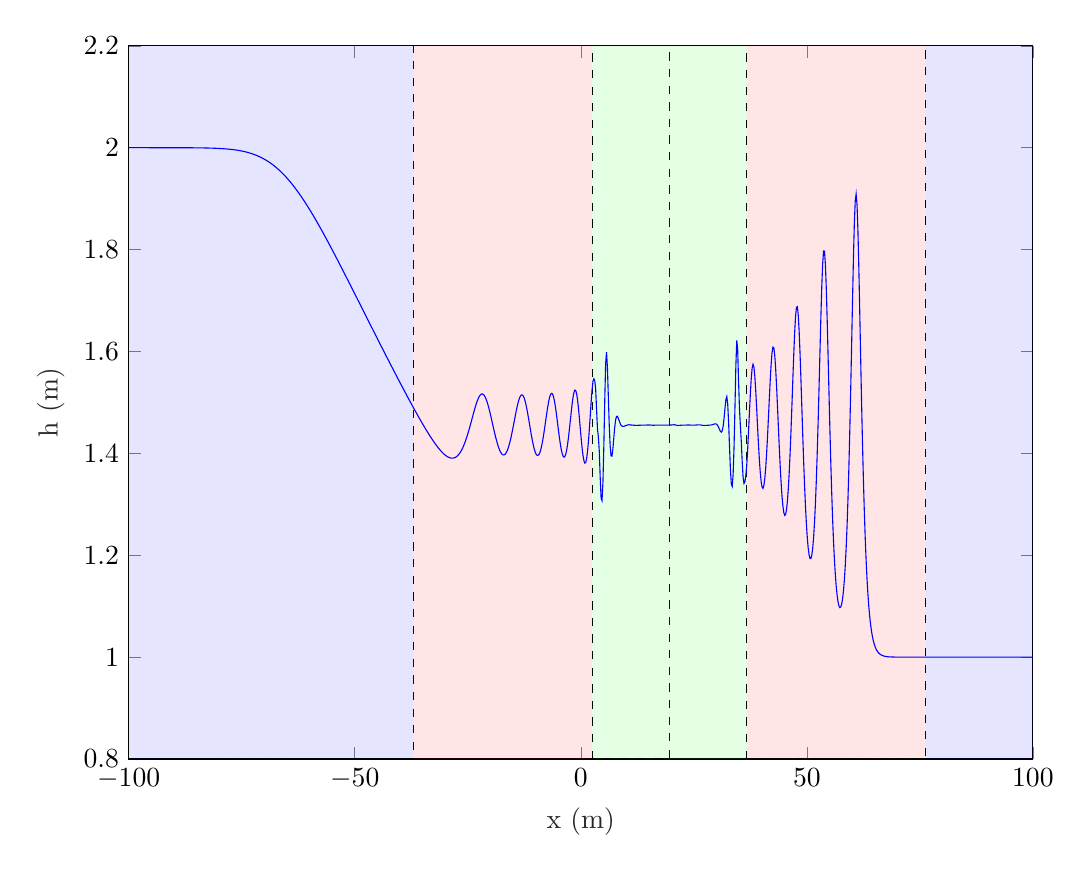
\begin{tikzpicture}

\begin{axis}[%
width=4.521in,
height=3.566in,
at={(0.758in,0.481in)},
scale only axis,
xmin=-100,
xmax=100,
xtick={-100,  -50,    0,   50,  100},
xlabel style={font=\color{white!15!black}},
xlabel={x (m)},
ymin=0.8,
ymax=2.2,
ytick={0.8,   1, 1.2, 1.4, 1.6, 1.8,   2, 2.2},
ylabel style={font=\color{white!15!black}},
ylabel={h (m)},
axis background/.style={fill=white}
]

\addplot[area legend, dashed, draw=black, fill=blue, fill opacity=0.1, forget plot]
table[row sep=crcr] {%
x	y\\
-100	0.8\\
-100	2.2\\
-37.0630892039997	2.2\\
-37.0630892039997	0.8\\
}--cycle;

\addplot[area legend, draw=none, fill=red, fill opacity=0.1, forget plot]
table[row sep=crcr] {%
x	y\\
-37.0630892039997	0.8\\
-37.0630892039997	2.2\\
2.50779195864934	2.2\\
2.50779195864934	0.8\\
}--cycle;

\addplot[area legend, dashed, draw=black, fill=green, fill opacity=0.1, forget plot]
table[row sep=crcr] {%
x	y\\
2.50779195864934	0.8\\
2.50779195864934	2.2\\
19.5890566189392	2.2\\
19.5890566189392	0.8\\
}--cycle;

\addplot[area legend, draw=none, fill=green, fill opacity=0.1, forget plot]
table[row sep=crcr] {%
x	y\\
19.5890566189392	0.8\\
19.5890566189392	2.2\\
36.670321279229	2.2\\
36.670321279229	0.8\\
}--cycle;

\addplot[area legend, dashed, draw=black, fill=red, fill opacity=0.1, forget plot]
table[row sep=crcr] {%
x	y\\
36.670321279229	0.8\\
36.670321279229	2.2\\
76.2412024418781	2.2\\
76.2412024418781	0.8\\
}--cycle;

\addplot[area legend, draw=none, fill=blue, fill opacity=0.1, forget plot]
table[row sep=crcr] {%
x	y\\
76.2412024418781	0.8\\
76.2412024418781	2.2\\
100	2.2\\
100	0.8\\
}--cycle;
\addplot [color=blue, forget plot]
  table[row sep=crcr]{%
-100.1200120012	2\\
-99.9199919991999	1.99999950092733\\
-99.7199719971997	1.99999896308632\\
-99.5199519951995	1.99999866455601\\
-99.3199319931993	1.99999848940598\\
-99.1199119911991	1.99999837441078\\
-98.9198919891989	1.99999828563001\\
-98.7198719871987	1.99999820475942\\
-98.5198519851985	1.9999981218163\\
-98.3198319831983	1.99999803122273\\
-98.1198119811981	1.99999792970955\\
-97.9197919791979	1.99999781519501\\
-97.7197719771977	1.99999768618431\\
-97.5197519751975	1.9999975414474\\
-97.3197319731973	1.99999737984489\\
-97.1197119711971	1.99999720023288\\
-96.9196919691969	1.99999700140929\\
-96.7196719671967	1.99999678208221\\
-96.5196519651965	1.99999654084953\\
-96.3196319631963	1.99999627618424\\
-96.1196119611961	1.99999598642247\\
-95.9195919591959	1.99999566975255\\
-95.7195719571957	1.99999532420429\\
-95.5195519551955	1.9999949476379\\
-95.3195319531953	1.99999453773245\\
-95.1195119511951	1.99999409197348\\
-94.9194919491949	1.9999936076398\\
-94.7194719471947	1.99999308178931\\
-94.5194519451945	1.99999251124385\\
-94.3194319431943	1.99999189257294\\
-94.1194119411941	1.99999122207631\\
-93.9193919391939	1.99999049576529\\
-93.7193719371937	1.9999897093428\\
-93.5193519351935	1.99998885818211\\
-93.3193319331933	1.99998793730399\\
-93.1193119311931	1.99998694135245\\
-92.9192919291929	1.99998586456877\\
-92.7192719271927	1.99998470076389\\
-92.5192519251925	1.99998344328894\\
-92.3192319231923	1.99998208500391\\
-92.1192119211921	1.99998061824425\\
-91.9191919191919	1.99997903478546\\
-91.7191719171917	1.99997732580529\\
-91.5191519151915	1.99997548184373\\
-91.3191319131913	1.99997349276047\\
-91.1191119111911	1.99997134768973\\
-90.9190919091909	1.99996903499243\\
-90.7190719071907	1.99996654220538\\
-90.5190519051905	1.99996385598758\\
-90.3190319031903	1.99996096206323\\
-90.1190119011901	1.99995784516151\\
-89.9189918991899	1.99995448895285\\
-89.7189718971897	1.99995087598158\\
-89.5189518951895	1.99994698759474\\
-89.3189318931893	1.99994280386694\\
-89.1189118911891	1.9999383035211\\
-88.9188918891889	1.99993346384478\\
-88.7188718871887	1.9999282606021\\
-88.5188518851885	1.99992266794088\\
-88.3188318831883	1.99991665829494\\
-88.1188118811881	1.99991020228133\\
-87.9187918791879	1.99990326859228\\
-87.7187718771877	1.99989582388168\\
-87.5187518751875	1.99988783264595\\
-87.3187318731873	1.99987925709907\\
-87.1187118711871	1.99987005704152\\
-86.9186918691869	1.99986018972309\\
-86.7186718671867	1.9998496096992\\
-86.5186518651865	1.99983826868073\\
-86.3186318631863	1.99982611537703\\
-86.1186118611861	1.99981309533203\\
-85.9185918591859	1.99979915075327\\
-85.7185718571857	1.99978422033371\\
-85.5185518551855	1.99976823906616\\
-85.3185318531853	1.9997511380503\\
-85.1185118511851	1.99973284429197\\
-84.9184918491849	1.9997132804949\\
-84.7184718471847	1.99969236484469\\
-84.5184518451845	1.99967001078488\\
-84.3184318431843	1.99964612678535\\
-84.1184118411841	1.99962061610284\\
-83.9183918391839	1.99959337653361\\
-83.7183718371837	1.99956430015859\\
-83.5183518351835	1.99953327308069\\
-83.3183318331833	1.99950017515479\\
-83.1183118311831	1.99946487971041\\
-82.9182918291829	1.99942725326726\\
-82.7182718271827	1.99938715524406\\
-82.5182518251825	1.99934443766084\\
-82.3182318231823	1.99929894483521\\
-82.1182118211821	1.9992505130729\\
-81.9181918191819	1.9991989703532\\
-81.7181718171817	1.99914413600974\\
-81.5181518151815	1.99908582040733\\
-81.3181318131813	1.99902382461557\\
-81.1181118111811	1.9989579400798\\
-80.9180918091809	1.99888794829058\\
-80.7180718071807	1.99881362045227\\
-80.5180518051805	1.99873471715203\\
-80.3180318031803	1.99865098803003\\
-80.1180118011801	1.99856217145234\\
-79.9179917991799	1.99846799418753\\
-79.7179717971797	1.99836817108851\\
-79.5179517951795	1.99826240478089\\
-79.3179317931793	1.99815038535953\\
-79.1179117911791	1.99803179009485\\
-78.9178917891789	1.99790628315056\\
-78.7178717871787	1.99777351531469\\
-78.5178517851785	1.99763312374575\\
-78.3178317831783	1.99748473173598\\
-78.1178117811781	1.99732794849376\\
-77.9177917791779	1.99716236894724\\
-77.7177717771777	1.9969875735714\\
-77.5177517751775	1.99680312824081\\
-77.3177317731773	1.99660858411024\\
-77.1177117711771	1.99640347752565\\
-76.9176917691769	1.99618732996765\\
-76.7176717671767	1.99595964803016\\
-76.5176517651765	1.9957199234363\\
-76.3176317631763	1.99546763309413\\
-76.1176117611761	1.99520223919449\\
-75.9175917591759	1.99492318935332\\
-75.7175717571757	1.99462991680069\\
-75.5175517551755	1.99432184061881\\
-75.3175317531753	1.993998366031\\
-75.1175117511751	1.99365888474381\\
-74.9174917491749	1.99330277534398\\
-74.7174717471747	1.99292940375208\\
-74.5174517451745	1.99253812373436\\
-74.3174317431743	1.99212827747412\\
-74.1174117411741	1.9916991962038\\
-73.9173917391739	1.99125020089869\\
-73.7173717371737	1.99078060303284\\
-73.5173517351735	1.99028970539758\\
-73.3173317331733	1.98977680298278\\
-73.1173117311731	1.98924118392043\\
-72.9172917291729	1.9886821304901\\
-72.7172717271727	1.9880989201852\\
-72.5172517251725	1.98749082683886\\
-72.3172317231723	1.98685712180752\\
-72.1172117211721	1.98619707521036\\
-71.9171917191719	1.98550995722185\\
-71.7171717171717	1.98479503941464\\
-71.5171517151715	1.98405159614943\\
-71.3171317131713	1.98327890600802\\
-71.1171117111711	1.98247625326554\\
-70.9170917091709	1.98164292939717\\
-70.7170717071707	1.98077823461455\\
-70.5170517051705	1.97988147942648\\
-70.3170317031703	1.97895198621843\\
-70.1170117011701	1.97798909084475\\
-69.9169916991699	1.97699214422735\\
-69.7169716971697	1.97596051395448\\
-69.5169516951695	1.97489358587263\\
-69.3169316931693	1.9737907656648\\
-69.1169116911691	1.97265148040797\\
-68.9168916891689	1.97147518010261\\
-68.7168716871687	1.97026133916701\\
-68.5168516851685	1.96900945788907\\
-68.3168316831683	1.96771906382861\\
-68.1168116811681	1.96638971316281\\
-67.9167916791679	1.96502099196807\\
-67.7167716771677	1.96361251743142\\
-67.5167516751675	1.96216393898515\\
-67.3167316731673	1.9606749393584\\
-67.1167116711671	1.95914523553996\\
-66.9166916691669	1.95757457964701\\
-66.7166716671667	1.95596275969472\\
-66.5166516651665	1.95430960026259\\
-66.3166316631663	1.95261496305337\\
-66.1166116611661	1.95087874734156\\
-65.9165916591659	1.94910089030868\\
-65.7165716571657	1.94728136726339\\
-65.5165516551655	1.94542019174504\\
-65.3165316531653	1.94351741550998\\
-65.1165116511651	1.9415731284006\\
-64.9164916491649	1.93958745809778\\
-64.7164716471647	1.93756056975813\\
-64.5164516451645	1.93549266553795\\
-64.3164316431643	1.93338398400652\\
-64.1164116411641	1.93123479945221\\
-63.9163916391639	1.92904542108502\\
-63.7163716371637	1.9268161921401\\
-63.5163516351635	1.9245474888873\\
-63.3163316331633	1.92223971955205\\
-63.1163116311631	1.91989332315347\\
-62.9162916291629	1.91750876826612\\
-62.7162716271627	1.91508655171184\\
-62.5162516251625	1.91262719718868\\
-62.3162316231623	1.91013125384398\\
-62.1162116211621	1.90759929479893\\
-61.9161916191619	1.90503191563203\\
-61.7161716171617	1.90242973282882\\
-61.5161516151615	1.89979338220558\\
-61.3161316131613	1.8971235173141\\
-61.1161116111611	1.89442080783514\\
-60.9160916091609	1.89168593796762\\
-60.7160716071607	1.88891960482041\\
-60.5160516051605	1.88612251681377\\
-60.3160316031603	1.88329539209651\\
-60.1160116011601	1.88043895698534\\
-59.9159915991599	1.87755394443201\\
-59.7159715971597	1.87464109252375\\
-59.5159515951595	1.87170114302209\\
-59.3159315931593	1.86873483994453\\
-59.1159115911591	1.86574292819343\\
-58.9158915891589	1.8627261522358\\
-58.7158715871587	1.85968525483725\\
-58.5158515851585	1.85662097585315\\
-58.3158315831583	1.85353405107925\\
-58.1158115811581	1.85042521116383\\
-57.9157915791579	1.84729518058306\\
-57.7157715771577	1.84414467668051\\
-57.5157515751575	1.84097440877184\\
-57.3157315731573	1.83778507731478\\
-57.1157115711571	1.8345773731447\\
-56.9156915691569	1.83135197677511\\
-56.7156715671567	1.82810955776284\\
-56.5156515651565	1.82485077413667\\
-56.3156315631563	1.82157627188823\\
-56.1156115611561	1.81828668452392\\
-55.9155915591559	1.81498263267596\\
-55.7155715571557	1.81166472377076\\
-55.5155515551555	1.80833355175268\\
-55.3155315531553	1.80498969686079\\
-55.1155115511551	1.80163372545651\\
-54.9154915491549	1.79826618989966\\
-54.7154715471547	1.79488762847039\\
-54.5154515451545	1.79149856533449\\
-54.3154315431543	1.78809951054955\\
-54.1154115411541	1.78469096010931\\
-53.9153915391539	1.78127339602365\\
-53.7153715371537	1.77784728643166\\
-53.5153515351535	1.77441308574526\\
-53.3153315331533	1.77097123482074\\
-53.1153115311531	1.7675221611561\\
-52.9152915291529	1.76406627911142\\
-52.7152715271527	1.76060399015037\\
-52.5152515251525	1.75713568310031\\
-52.3152315231523	1.75366173442911\\
-52.1152115211521	1.75018250853658\\
-51.9151915191519	1.74669835805863\\
-51.7151715171517	1.74320962418228\\
-51.5151515151515	1.73971663696994\\
-51.3151315131513	1.73621971569131\\
-51.1151115111511	1.7327191691614\\
-50.9150915091509	1.72921529608336\\
-50.7150715071507	1.72570838539486\\
-50.5150515051505	1.72219871661676\\
-50.3150315031503	1.71868656020328\\
-50.1150115011501	1.7151721778924\\
-49.9149914991499	1.711655823056\\
-49.7149714971497	1.70813774104872\\
-49.5149514951495	1.70461816955506\\
-49.3149314931493	1.7010973389342\\
-49.1149114911491	1.69757547256195\\
-48.9148914891489	1.69405278716956\\
-48.7148714871487	1.69052949317909\\
-48.5148514851485	1.68700579503515\\
-48.3148314831483	1.68348189153281\\
-48.1148114811481	1.67995797614172\\
-47.9147914791479	1.67643423732635\\
-47.7147714771477	1.67291085886256\\
-47.5147514751475	1.66938802015051\\
-47.3147314731473	1.66586589652419\\
-47.1147114711471	1.66234465955784\\
-46.9146914691469	1.65882447736956\\
-46.7146714671467	1.65530551492252\\
-46.5146514651465	1.65178793432414\\
-46.3146314631463	1.64827189512384\\
-46.1146114611461	1.64475755460984\\
-45.9145914591459	1.64124506810555\\
-45.7145714571457	1.63773458926636\\
-45.5145514551455	1.63422627037743\\
-45.3145314531453	1.63072026265327\\
-45.1145114511451	1.6272167165399\\
-44.9144914491449	1.62371578202064\\
-44.7144714471447	1.62021760892626\\
-44.5144514451445	1.61672234725067\\
-44.3144314431443	1.61323014747318\\
-44.1144114411441	1.6097411608886\\
-43.9143914391439	1.60625553994623\\
-43.7143714371437	1.60277343859934\\
-43.5143514351435	1.59929501266641\\
-43.3143314331433	1.59582042020576\\
-43.1143114311431	1.59234982190518\\
-42.9142914291429	1.58888338148843\\
-42.7142714271427	1.58542126614046\\
-42.5142514251425	1.58196364695346\\
-42.3142314231423	1.57851069939605\\
-42.1142114211421	1.57506260380783\\
-41.9141914191419	1.57161954592219\\
-41.7141714171417	1.56818171741997\\
-41.5141514151415	1.56474931651712\\
-41.3141314131413	1.56132254858979\\
-41.1141114111411	1.55790162684027\\
-40.9140914091409	1.55448677300784\\
-40.7140714071407	1.55107821812882\\
-40.5140514051405	1.54767620335029\\
-40.3140314031403	1.54428098080276\\
-40.1140114011401	1.54089281453708\\
-39.9139913991399	1.53751198153182\\
-39.7139713971397	1.53413877277744\\
-39.5139513951395	1.53077349444464\\
-39.3139313931393	1.52741646914442\\
-39.1139113911391	1.52406803728867\\
-38.9138913891389	1.5207285585604\\
-38.7138713871387	1.51739841350387\\
-38.5138513851385	1.51407800524572\\
-38.3138313831383	1.51076776135929\\
-38.1138113811381	1.50746813588544\\
-37.9137913791379	1.50417961152435\\
-37.7137713771377	1.50090270201421\\
-37.5137513751375	1.49763795471419\\
-37.3137313731373	1.49438595341064\\
-37.1137113711371	1.49114732136716\\
-36.9136913691369	1.48792272464124\\
-36.7136713671367	1.48471287569211\\
-36.5136513651365	1.48151853730658\\
-36.3136313631363	1.47834052687222\\
-36.1136113611361	1.47517972102972\\
-35.9135913591359	1.47203706073897\\
-35.7135713571357	1.46891355679641\\
-35.5135513551355	1.46581029584423\\
-35.3135313531353	1.46272844691548\\
-35.1135113511351	1.45966926856234\\
-34.9134913491349	1.45663411661857\\
-34.7134713471347	1.45362445265069\\
-34.5134513451345	1.45064185315629\\
-34.3134313431343	1.44768801957157\\
-34.1134113411341	1.44476478915359\\
-33.9133913391339	1.4418741468063\\
-33.7133713371337	1.43901823792247\\
-33.5133513351335	1.43619938231574\\
-33.3133313331333	1.43342008931886\\
-33.1133113311331	1.43068307412477\\
-32.9132913291329	1.42799127544586\\
-32.7132713271327	1.42534787456406\\
-32.5132513251325	1.42275631583879\\
-32.3132313231323	1.42022032873104\\
-32.1132113211321	1.41774395138905\\
-31.9131913191319	1.41533155582274\\
-31.7131713171317	1.41298787467029\\
-31.5131513151315	1.41071802952708\\
-31.3131313131313	1.40852756076593\\
-31.1131113111311	1.40642245872337\\
-30.9130913091309	1.40440919605891\\
-30.7130713071307	1.40249476100919\\
-30.5130513051305	1.40068669115338\\
-30.3130313031303	1.39899310717688\\
-30.1130113011301	1.39742274596279\\
-29.9129912991299	1.39598499214999\\
-29.7129712971297	1.39468990706882\\
-29.5129512951295	1.39354825369456\\
-29.3129312931293	1.39257151593996\\
-29.1129112911291	1.39177191023706\\
-28.9128912891289	1.39116238693059\\
-28.7128712871287	1.39075661851861\\
-28.5128512851285	1.3905689660827\\
-28.3128312831283	1.39061457493451\\
-28.1128112811281	1.3909089255804\\
-27.9127912791279	1.39146803711155\\
-27.7127712771277	1.39230827428596\\
-27.5127512751275	1.39344613120957\\
-27.3127312731273	1.39489801995333\\
-27.1127112711271	1.39667992364866\\
-26.9126912691269	1.39880707950477\\
-26.7126712671267	1.40129352960032\\
-26.5126512651265	1.40415156784694\\
-26.3126312631263	1.40739119269163\\
-26.1126112611261	1.4110193665671\\
-25.9125912591259	1.41503922993595\\
-25.7125712571257	1.41944928383902\\
-25.5125512551255	1.42424238080916\\
-25.3125312531253	1.42940477137978\\
-25.1125112511251	1.43491510524948\\
-24.9124912491249	1.44074337493801\\
-24.7124712471247	1.44685005224975\\
-24.5124512451245	1.45318526649364\\
-24.3124312431243	1.45968823293254\\
-24.1124112411241	1.46628698077278\\
-23.9123912391239	1.47289849900344\\
-23.7123712371237	1.47942930197073\\
-23.5123512351235	1.48577663392502\\
-23.3123312331233	1.49183028651852\\
-23.1123112311231	1.49747500411395\\
-22.9122912291229	1.50259362356516\\
-22.7122712271227	1.50707072756168\\
-22.5122512251225	1.51079668887714\\
-22.3122312231223	1.51367203638528\\
-22.1122112211221	1.5156117156728\\
-21.9121912191219	1.51654905310722\\
-21.7121712171217	1.51643907969443\\
-21.5121512151215	1.51526183103799\\
-21.3121312131213	1.5130230983142\\
-21.1121112111211	1.50975492693953\\
-20.9120912091209	1.50551485151855\\
-20.7120712071207	1.5003838960842\\
-20.5120512051205	1.49446350640095\\
-20.3120312031203	1.48787189567957\\
-20.1120112011201	1.48073994496669\\
-19.9119911991199	1.47320687417978\\
-19.7119711971197	1.46541602373747\\
-19.5119511951195	1.45751105094492\\
-19.3119311931193	1.44963266732225\\
-19.1119111911191	1.44191595170203\\
-18.9118911891189	1.43448829537956\\
-18.7118711871187	1.42746802464366\\
-18.5118511851185	1.4209636050717\\
-18.3118311831183	1.41507331980976\\
-18.1118111811181	1.40988528123492\\
-17.9117911791179	1.40547767953464\\
-17.7117711771177	1.40191912966596\\
-17.5117511751175	1.39926900492101\\
-17.3117311731173	1.39757760895913\\
-17.1117111711171	1.39688429139296\\
-16.9116911691169	1.39722647515201\\
-16.7116711671167	1.39861931981814\\
-16.5116511651165	1.40107403438673\\
-16.3116311631163	1.40458641003825\\
-16.1116111611161	1.40913642113233\\
-15.9115911591159	1.41468545032929\\
-15.7115711571157	1.42117326596033\\
-15.5115511551155	1.42851487725013\\
-15.3115311531153	1.4365975944688\\
-15.1115111511151	1.44527847806394\\
-14.9114911491149	1.45438276473766\\
-14.7114711471147	1.46370386872913\\
-14.5114511451145	1.47300521989781\\
-14.3114311431143	1.48202468068253\\
-14.1114111411141	1.4904818512355\\
-13.9113911391139	1.49808830731171\\
-13.7113711371137	1.50456068960722\\
-13.5113511351135	1.50963587953516\\
-13.3113311331133	1.51308723559047\\
-13.1113111311131	1.51474014403958\\
-12.9112911291129	1.51448531758543\\
-12.7112711271127	1.51229086053232\\
-12.5112511251125	1.50820422011802\\
-12.3112311231123	1.50235230909853\\
-12.1112111211121	1.49493483493154\\
-11.9111911191119	1.48621256889159\\
-11.7111711171117	1.47649322584471\\
-11.5111511151115	1.46611460897952\\
-11.3111311131113	1.45542844095852\\
-11.1111111111111	1.44478580942741\\
-10.9110911091109	1.43452468205384\\
-10.7110711071107	1.42496037072912\\
-10.5110511051105	1.41637891914392\\
-10.3110311031103	1.40903292494401\\
-10.1110111011101	1.40313919088828\\
-9.91099109910991	1.39887761357129\\
-9.71097109710971	1.39639045141289\\
-9.5109510951095	1.3957844265317\\
-9.3109310931093	1.39711339742929\\
-9.1109110911091	1.40040348470073\\
-8.9108910891089	1.40562064691021\\
-8.7108710871087	1.4126778184992\\
-8.51085108510851	1.42142450314662\\
-8.31083108310831	1.43163895658816\\
-8.11081108110811	1.44302133571646\\
-7.91079107910791	1.45518979746287\\
-7.71077107710771	1.46768170236583\\
-7.51075107510751	1.47996236380442\\
-7.31073107310731	1.49144365929059\\
-7.1107110711071	1.50151396307193\\
-6.9106910691069	1.50957854824756\\
-6.7106710671067	1.51510851002079\\
-6.5106510651065	1.51769281301356\\
-6.3106310631063	1.51707729445229\\
-6.11061106110611	1.51321785349944\\
-5.91059105910591	1.50627281742691\\
-5.71057105710571	1.49660385432861\\
-5.51055105510551	1.48474415850392\\
-5.31053105310531	1.47135321589488\\
-5.11051105110511	1.4571641620341\\
-4.91049104910491	1.4429321524224\\
-4.7104710471047	1.42938987964094\\
-4.5104510451045	1.41721300307546\\
-4.3104310431043	1.40699736455477\\
-4.1104110411041	1.3992439917419\\
-3.9103910391039	1.39435083243218\\
-3.71037103710371	1.39260464262582\\
-3.51035103510351	1.39418940944172\\
-3.31033103310331	1.39914104077392\\
-3.11031103110311	1.40736925090253\\
-2.91029102910291	1.41861899285776\\
-2.71027102710271	1.43245101342906\\
-2.51025102510251	1.44822074057783\\
-2.3102310231023	1.46506655451811\\
-2.1102110211021	1.48191888350632\\
-1.9101910191019	1.49754207118168\\
-1.7101710171017	1.51061878227216\\
-1.5101510151015	1.51988110547336\\
-1.31013101310131	1.52427954201963\\
-1.11011101110111	1.52312647303146\\
-0.91009100910091	1.51630236428631\\
-0.710071007100709	1.50423603405536\\
-0.510051005100507	1.48790058563379\\
-0.310031003100306	1.4686799507291\\
-0.110011001100105	1.44819485944954\\
0.0900090009000962	1.42812484466475\\
0.290029002900297	1.41006348165341\\
0.490049004900499	1.39541759598036\\
0.6900690069007	1.38535026145926\\
0.890089008900901	1.3807462195281\\
1.09010901090109	1.38222466480084\\
1.29012901290129	1.39002760496606\\
1.49014901490149	1.40404733831749\\
1.69016901690169	1.42370267998915\\
1.89018901890189	1.44783441771924\\
2.09020902090209	1.47458338326238\\
2.2902290229023	1.50132003977679\\
2.4902490249025	1.52491191926622\\
2.6902690269027	1.54156454428223\\
2.8902890289029	1.54642665800627\\
3.0903090309031	1.54237452465847\\
3.2903290329033	1.52551270662569\\
3.4903490349035	1.48487380873849\\
3.69036903690369	1.44778480952842\\
3.89038903890389	1.43154422467913\\
4.09040904090409	1.4030713617025\\
4.29042904290429	1.35184494230331\\
4.49044904490449	1.31201714541919\\
4.6904690469047	1.30722003726545\\
4.8904890489049	1.3426002598265\\
5.0905090509051	1.41307701346819\\
5.2905290529053	1.50207844791207\\
5.4905490549055	1.57648742052323\\
5.6905690569057	1.59868942348001\\
5.8905890589059	1.56742471065623\\
6.09060906090609	1.51020077913597\\
6.29062906290629	1.45442669586424\\
6.49064906490649	1.41445427236947\\
6.69066906690669	1.39492733061817\\
6.89068906890689	1.39454522630394\\
7.0907090709071	1.40835791397949\\
7.2907290729073	1.42938573960437\\
7.4907490749075	1.45017863059563\\
7.6907690769077	1.46516851245064\\
7.8907890789079	1.47229213408864\\
8.0908090809081	1.47277805804732\\
8.2908290829083	1.46907699597859\\
8.49084908490849	1.46382025914771\\
8.69086908690869	1.45901891120216\\
8.89088908890889	1.45552545336532\\
9.09090909090909	1.45356251061693\\
9.29092909290929	1.45286365013244\\
9.4909490949095	1.45300887225311\\
9.6909690969097	1.45360656803275\\
9.8909890989099	1.45434488957776\\
10.0910091009101	1.45500131807467\\
10.2910291029103	1.45552828550359\\
10.4910491049105	1.45596062339078\\
10.6910691069107	1.45615395078531\\
10.8910891089109	1.45591463570006\\
11.0911091109111	1.45562659180956\\
11.2911291129113	1.45557243934361\\
11.4911491149115	1.45542734360368\\
11.6911691169117	1.45523105336008\\
11.8911891189119	1.45508775026456\\
12.0912091209121	1.45500372772503\\
12.2912291229123	1.45498007272372\\
12.4912491249125	1.45500836942596\\
12.6912691269127	1.45507568172372\\
12.8912891289129	1.45516028102107\\
13.0913091309131	1.45523313681441\\
13.2913291329133	1.45528509055348\\
13.4913491349135	1.45533288725628\\
13.6913691369137	1.45536395913297\\
13.8913891389139	1.45541465054792\\
14.0914091409141	1.4554673317141\\
14.2914291429143	1.45547993768375\\
14.4914491449145	1.45551655311873\\
14.6914691469147	1.45561200175496\\
14.8914891489149	1.45573424815264\\
15.0915091509151	1.45576344508366\\
15.2915291529153	1.45564807648876\\
15.4915491549155	1.45545605408599\\
15.6915691569157	1.45529922466869\\
15.8915891589159	1.45524167976987\\
16.0916091609161	1.45522626432073\\
16.2916291629163	1.45524377993837\\
16.4916491649165	1.45539343543431\\
16.6916691669167	1.45554429585994\\
16.8916891689169	1.45554261057587\\
17.0917091709171	1.45551740046874\\
17.2917291729173	1.45548985114544\\
17.4917491749175	1.45546554533378\\
17.6917691769177	1.45546414837133\\
17.8917891789179	1.4554710160197\\
18.0918091809181	1.45547684079071\\
18.2918291829183	1.45546077075719\\
18.4918491849185	1.45540778480355\\
18.6918691869187	1.45534841944975\\
18.8918891889189	1.45533038036821\\
19.0919091909191	1.45536230056509\\
19.2919291929193	1.45541025975063\\
19.4919491949195	1.45545289464914\\
19.6919691969197	1.45550901703382\\
19.8919891989199	1.45560451680553\\
20.0920092009201	1.45573746811342\\
20.2920292029203	1.45592913882229\\
20.4920492049205	1.45611442122753\\
20.6920692069207	1.45611525220327\\
20.8920892089209	1.45584048571175\\
21.0921092109211	1.45538913537894\\
21.2921292129213	1.45497847066885\\
21.4921492149215	1.4547948318947\\
21.6921692169217	1.45485359229608\\
21.8921892189219	1.45500901276755\\
22.0922092209221	1.4551363285858\\
22.2922292229223	1.45525547695787\\
22.4922492249225	1.45537998094536\\
22.6922692269227	1.45544505912965\\
22.8922892289229	1.4554688781373\\
23.0923092309231	1.45549845555842\\
23.2923292329233	1.45553055351336\\
23.4923492349235	1.4555761080189\\
23.6923692369237	1.45563090578376\\
23.8923892389239	1.45564232655067\\
24.0924092409241	1.45558631877258\\
24.2924292429243	1.45549343124201\\
24.4924492449245	1.45540083662468\\
24.6924692469247	1.45533279284321\\
24.8924892489249	1.45532995412647\\
25.0925092509251	1.45539079853218\\
25.2925292529253	1.45549494109034\\
25.4925492549255	1.45561365289943\\
25.6925692569257	1.45572360252783\\
25.8925892589259	1.45586010189638\\
26.0926092609261	1.45599589803344\\
26.2926292629263	1.45600285301601\\
26.4926492649265	1.45579809560654\\
26.6926692669267	1.45542275664451\\
26.8926892689269	1.45503444516378\\
27.0927092709271	1.45479985897316\\
27.2927292729273	1.45477273506505\\
27.4927492749275	1.45486980778665\\
27.6927692769277	1.45496029559467\\
27.8927892789279	1.45501655998384\\
28.0928092809281	1.45510357475734\\
28.2928292829283	1.45523463345766\\
28.4928492849285	1.45537241711965\\
28.6928692869287	1.45554643619197\\
28.8928892889289	1.45584600514722\\
29.0929092909291	1.45630728807539\\
29.2929292929293	1.45688370794517\\
29.4929492949295	1.4574839889347\\
29.6929692969297	1.45791107281226\\
29.8929892989299	1.45779312811513\\
30.0930093009301	1.45672190696912\\
30.2930293029303	1.45441519114916\\
30.4930493049305	1.45087354467921\\
30.6930693069307	1.44662674263775\\
30.8930893089309	1.44292691196857\\
31.0931093109311	1.44159770252286\\
31.2931293129313	1.44477737758383\\
31.4931493149315	1.45406300745419\\
31.6931693169317	1.46957605678406\\
31.8931893189319	1.48895292578166\\
32.0932093209321	1.506068225298\\
32.2932293229323	1.51148623484825\\
32.4932493249325	1.49655878142507\\
32.6932693269327	1.46057040954931\\
32.8932893289329	1.41285981624429\\
33.0933093309331	1.36816574916297\\
33.2933293329333	1.33945764569469\\
33.4933493349335	1.33503078442236\\
33.6933693369337	1.35935189383838\\
33.8933893389339	1.41249046295992\\
34.0934093409341	1.48880665209869\\
34.2934293429343	1.57098196894304\\
34.4934493449345	1.6217505798928\\
34.6934693469347	1.6043533227473\\
34.8934893489349	1.54173827297502\\
35.0935093509351	1.48749588285881\\
35.2935293529353	1.45434683179171\\
35.4935493549355	1.42364961433921\\
35.6935693569357	1.38417783551091\\
35.8935893589359	1.35296980862965\\
36.0936093609361	1.34082853096418\\
36.2936293629363	1.34413670598739\\
36.4936493649365	1.35628634338893\\
36.6936693669367	1.37631864457075\\
36.8936893689369	1.40550741907328\\
37.0937093709371	1.44129138749262\\
37.2937293729373	1.47936120719399\\
37.4937493749375	1.51583561323681\\
37.6937693769377	1.54647043074194\\
37.8937893789379	1.56712988101855\\
38.0938093809381	1.57491315139729\\
38.2938293829383	1.56902722991562\\
38.4938493849385	1.55057143722288\\
38.6938693869387	1.52255082166367\\
38.8938893889389	1.48872318377193\\
39.0939093909391	1.45287535497477\\
39.2939293929393	1.41829547485863\\
39.4939493949395	1.38755173538642\\
39.6939693969397	1.36248634319897\\
39.8939893989399	1.34432041005876\\
40.0940094009401	1.33378989786357\\
40.2940294029403	1.33123909966405\\
40.4940494049405	1.33683472134777\\
40.6940694069407	1.35032866913803\\
40.8940894089409	1.37129914402551\\
41.0941094109411	1.3989575221955\\
41.2941294129413	1.43207363661986\\
41.4941494149415	1.46886908239298\\
41.6941694169417	1.50694415517736\\
41.8941894189419	1.54330025580432\\
42.0942094209421	1.57453057540102\\
42.2942294229423	1.59723036520903\\
42.4942494249425	1.6085960156076\\
42.6942694269427	1.60706701267132\\
42.8942894289429	1.59266262308213\\
43.0943094309431	1.5670560667954\\
43.2943294329433	1.53304078773409\\
43.4943494349435	1.4939132847479\\
43.6943694369437	1.45290369589136\\
43.8943894389439	1.41280440438936\\
44.0944094409441	1.37581256312414\\
44.2944294429443	1.34353024839811\\
44.4944494449445	1.31705170322676\\
44.6944694469447	1.29708642005523\\
44.8944894489449	1.28407905764835\\
45.0945094509451	1.27831356553572\\
45.2945294529453	1.27996510643821\\
45.4945494549455	1.28917383440147\\
45.6945694569457	1.30600171280181\\
45.8945894589459	1.33041301590117\\
46.0946094609461	1.36218845999164\\
46.2946294629463	1.40079989713712\\
46.4946494649465	1.44524927102977\\
46.6946694669467	1.49388759002904\\
46.8946894689469	1.54424768992527\\
47.0947094709471	1.59296535283755\\
47.2947294729473	1.63588976410372\\
47.4947494749475	1.66850714883405\\
47.6947694769477	1.68672854016134\\
47.8947894789479	1.68789617771437\\
48.0948094809481	1.67148520407385\\
48.2948294829483	1.63942363961356\\
48.4948494849485	1.59536337668195\\
48.6948694869487	1.54372940735492\\
48.8948894889489	1.4888248619933\\
49.0949094909491	1.43426491207977\\
49.2949294929493	1.3827663566208\\
49.4949494949495	1.33616812262392\\
49.6949694969497	1.29558377869046\\
49.8949894989499	1.26158863066247\\
50.0950095009501	1.23440297883415\\
50.2950295029503	1.21404850280144\\
50.4950495049505	1.20046736176467\\
50.6950695069507	1.19361361521808\\
50.8950895089509	1.19350758103226\\
51.0951095109511	1.2002734756566\\
51.2951295129513	1.21414502825543\\
51.4951495149515	1.23544976217285\\
51.6951695169517	1.26456123230077\\
51.8951895189519	1.30181877401937\\
52.0952095209521	1.3473943359004\\
52.2952295229523	1.40111027415293\\
52.4952495249525	1.4621850870835\\
52.6952695269527	1.52893398810256\\
52.8952895289529	1.59843291889739\\
53.0953095309531	1.66626890729136\\
53.2953295329533	1.72652752181175\\
53.4953495349535	1.77234262434547\\
53.6953695369537	1.79722800511857\\
53.8953895389539	1.79703476091182\\
54.0954095409541	1.77143650299595\\
54.2954295429543	1.72426058528841\\
54.4954495449545	1.66184903527027\\
54.6954695469547	1.59108895540749\\
54.8954895489549	1.51799640507659\\
55.0955095509551	1.44709785759185\\
55.2955295529553	1.38137528232199\\
55.4955495549555	1.32252455755421\\
55.6955695569557	1.27126418437972\\
55.8955895589559	1.22766624977511\\
56.0956095609561	1.19139377354625\\
56.2956295629563	1.16191321968194\\
56.4956495649565	1.13861686301141\\
56.6956695669567	1.12092576641959\\
56.8956895689569	1.10834713221286\\
57.0957095709571	1.10050432390338\\
57.2957295729573	1.0971758467348\\
57.4957495749575	1.09827746992442\\
57.6957695769577	1.10391324037285\\
57.8957895789579	1.11433866847464\\
58.0958095809581	1.12998182056814\\
58.2958295829583	1.15143414682388\\
58.4958495849585	1.17941898013044\\
58.6958695869587	1.21477111654413\\
58.8958895889589	1.25834095930976\\
59.0959095909591	1.31089820453224\\
59.2959295929593	1.3729261366802\\
59.4959495949595	1.44436574998947\\
59.6959695969597	1.52423232059236\\
59.8959895989599	1.61015107450194\\
60.0960096009601	1.69782734908871\\
60.2960296029603	1.78064200262217\\
60.4960496049605	1.84972848390275\\
60.6960696069607	1.89522038201315\\
60.8960896089609	1.90909040169856\\
61.0961096109611	1.88839459590092\\
61.2961296129613	1.83703382673749\\
61.4961496149615	1.7637191272341\\
61.6961696169617	1.67830737118676\\
61.8961896189619	1.58931343928796\\
62.0962096209621	1.50291978005624\\
62.2962296229623	1.42301627009727\\
62.4962496249625	1.35165166594659\\
62.6962696269627	1.28955509013115\\
62.8962896289629	1.23659144493208\\
63.0963096309631	1.19211370698623\\
63.2963296329633	1.15521500060792\\
63.4963496349635	1.12489722198272\\
63.6963696369637	1.10017593372213\\
63.8963896389639	1.08013964037291\\
64.0964096409641	1.06397825230914\\
64.2964296429643	1.05099194837806\\
64.4964496449645	1.04058842678606\\
64.6964696469647	1.03227394413554\\
64.8964896489649	1.02564160854173\\
65.0965096509651	1.02035902825395\\
65.2965296529653	1.01615649969221\\
65.4965496549655	1.01281632888374\\
65.6965696569657	1.01016351835186\\
65.8965896589659	1.00805784164784\\
66.0966096609661	1.00638721545258\\
66.2966296629663	1.00506222715321\\
66.4966496649665	1.0040116593287\\
66.6966696669667	1.00317885586178\\
66.8966896689669	1.00251878765374\\
67.0967096709671	1.00199569331502\\
67.2967296729673	1.00158118841203\\
67.4967496749675	1.00125275410129\\
67.6967696769677	1.00099253144504\\
67.8967896789679	1.00078636109042\\
68.0968096809681	1.00062301931883\\
68.2968296829683	1.00049361089648\\
68.4968496849685	1.00039108690708\\
68.6968696869687	1.00030986206573\\
68.8968896889689	1.00024551112983\\
69.0969096909691	1.00019452814554\\
69.2969296929693	1.00015413557841\\
69.4969496949695	1.00012213302517\\
69.6969696969697	1.00009677731875\\
69.8969896989699	1.00007668752478\\
70.0970097009701	1.00006076966882\\
70.2970297029703	1.00004815710122\\
70.4970497049705	1.00003816325328\\
70.6970697069707	1.00003024421138\\
70.8970897089709	1.00002396906958\\
71.0971097109711	1.00001899644433\\
71.2971297129713	1.00001505587066\\
71.4971497149715	1.00001193306517\\
71.6971697169717	1.00000945825222\\
71.8971897189719	1.00000749691631\\
72.0972097209721	1.00000594247651\\
72.2972297229723	1.00000471048326\\
72.4972497249725	1.00000373402114\\
72.6972697269727	1.00000296006693\\
72.8972897289729	1.00000234660434\\
73.0973097309731	1.00000186033826\\
73.2973297329733	1.00000147488378\\
73.4973497349735	1.00000116933147\\
73.6973697369737	1.00000092711061\\
73.8973897389739	1.00000073508856\\
74.0974097409741	1.0000005828571\\
74.2974297429743	1.00000046216702\\
74.4974497449745	1.00000036648006\\
74.6974697469747	1.00000029061391\\
74.8974897489749	1.00000023046088\\
75.0975097509751	1.00000018276494\\
75.2975297529753	1.0000001449451\\
75.4975497549755	1.00000011495537\\
75.6975697569757	1.00000009117382\\
75.8975897589759	1.00000007231465\\
76.0976097609761	1.00000005735851\\
76.2976297629763	1.00000004549721\\
76.4976497649765	1.00000003609003\\
76.6976697669767	1.00000002862895\\
76.8976897689769	1.00000002271115\\
77.0977097709771	1.00000001801726\\
77.2977297729773	1.00000001429401\\
77.4977497749775	1.00000001134058\\
77.6977697769777	1.00000000899773\\
77.8977897789779	1.00000000713914\\
78.0978097809781	1.00000000566468\\
78.2978297829783	1.00000000449491\\
78.4978497849785	1.00000000356683\\
78.6978697869787	1.00000000283048\\
78.8978897889789	1.00000000224623\\
79.0979097909791	1.00000000178264\\
79.2979297929793	1.00000000141478\\
79.4979497949795	1.00000000112288\\
79.6979697969797	1.00000000089123\\
79.8979897989799	1.0000000007074\\
80.0980098009801	1.00000000056151\\
80.2980298029803	1.00000000044572\\
80.4980498049805	1.00000000035382\\
80.6980698069807	1.00000000028088\\
80.8980898089809	1.00000000022299\\
81.0981098109811	1.00000000017703\\
81.2981298129813	1.00000000014055\\
81.4981498149815	1.00000000011159\\
81.6981698169817	1.0000000000886\\
81.8981898189819	1.00000000007035\\
82.0982098209821	1.00000000005586\\
82.2982298229823	1.00000000004436\\
82.4982498249825	1.00000000003522\\
82.6982698269827	1.00000000002797\\
82.8982898289829	1.00000000002221\\
83.0983098309831	1.00000000001764\\
83.2983298329833	1.00000000001401\\
83.4983498349835	1.00000000001112\\
83.6983698369837	1.00000000000883\\
83.8983898389839	1.00000000000702\\
84.0984098409841	1.00000000000557\\
84.2984298429843	1.00000000000442\\
84.4984498449845	1.00000000000351\\
84.6984698469847	1.00000000000279\\
84.8984898489849	1.00000000000221\\
85.0985098509851	1.00000000000176\\
85.2985298529853	1.00000000000139\\
85.4985498549855	1.00000000000111\\
85.6985698569857	1.00000000000088\\
85.8985898589859	1.0000000000007\\
86.0986098609861	1.00000000000055\\
86.2986298629863	1.00000000000043\\
86.4986498649865	1.00000000000034\\
86.6986698669867	1.00000000000027\\
86.8986898689869	1.00000000000021\\
87.0987098709871	1.00000000000017\\
87.2987298729873	1.00000000000013\\
87.4987498749875	1.0000000000001\\
87.6987698769877	1.00000000000008\\
87.8987898789879	1.00000000000006\\
88.0988098809881	1.00000000000004\\
88.2988298829883	1.00000000000003\\
88.4988498849885	1.00000000000002\\
88.6988698869887	1.00000000000002\\
88.8988898889889	1.00000000000001\\
89.0989098909891	1.00000000000001\\
89.2989298929893	1\\
89.4989498949895	1\\
89.6989698969897	1\\
89.8989898989899	1\\
90.0990099009901	1\\
90.2990299029903	1\\
90.4990499049905	1\\
90.6990699069907	1\\
90.8990899089909	1\\
91.0991099109911	1\\
91.2991299129913	1\\
91.4991499149915	1\\
91.6991699169917	1\\
91.8991899189919	1\\
92.0992099209921	1\\
92.2992299229923	1\\
92.4992499249925	1\\
92.6992699269927	1\\
92.8992899289929	1\\
93.0993099309931	1\\
93.2993299329933	1\\
93.4993499349935	1\\
93.6993699369937	1\\
93.8993899389939	1\\
94.0994099409941	1\\
94.2994299429943	1\\
94.4994499449945	1\\
94.6994699469947	1\\
94.8994899489949	1\\
95.0995099509951	1\\
95.2995299529953	1\\
95.4995499549955	1\\
95.6995699569957	1\\
95.8995899589959	1\\
96.0996099609961	1\\
96.2996299629963	1\\
96.4996499649965	1\\
96.6996699669967	1\\
96.8996899689969	1\\
97.0997099709971	1\\
97.2997299729973	1\\
97.4997499749975	1\\
97.6997699769977	1\\
97.8997899789979	1\\
98.0998099809981	1\\
98.2998299829983	1\\
98.4998499849985	1\\
98.6998699869987	1\\
98.8998899889989	1\\
99.0999099909991	1\\
99.2999299929993	1\\
99.4999499949995	1\\
99.6999699969997	1\\
99.8999899989999	1\\
100.100010001	1\\
};
\end{axis}
\end{tikzpicture}%
		\caption{$h$}
	\end{subfigure}
	\begin{subfigure}{0.49\textwidth}
		\centering
		% This file was created by matlab2tikz.
%
%The latest updates can be retrieved from
%  http://www.mathworks.com/matlabcentral/fileexchange/22022-matlab2tikz-matlab2tikz
%where you can also make suggestions and rate matlab2tikz.
%
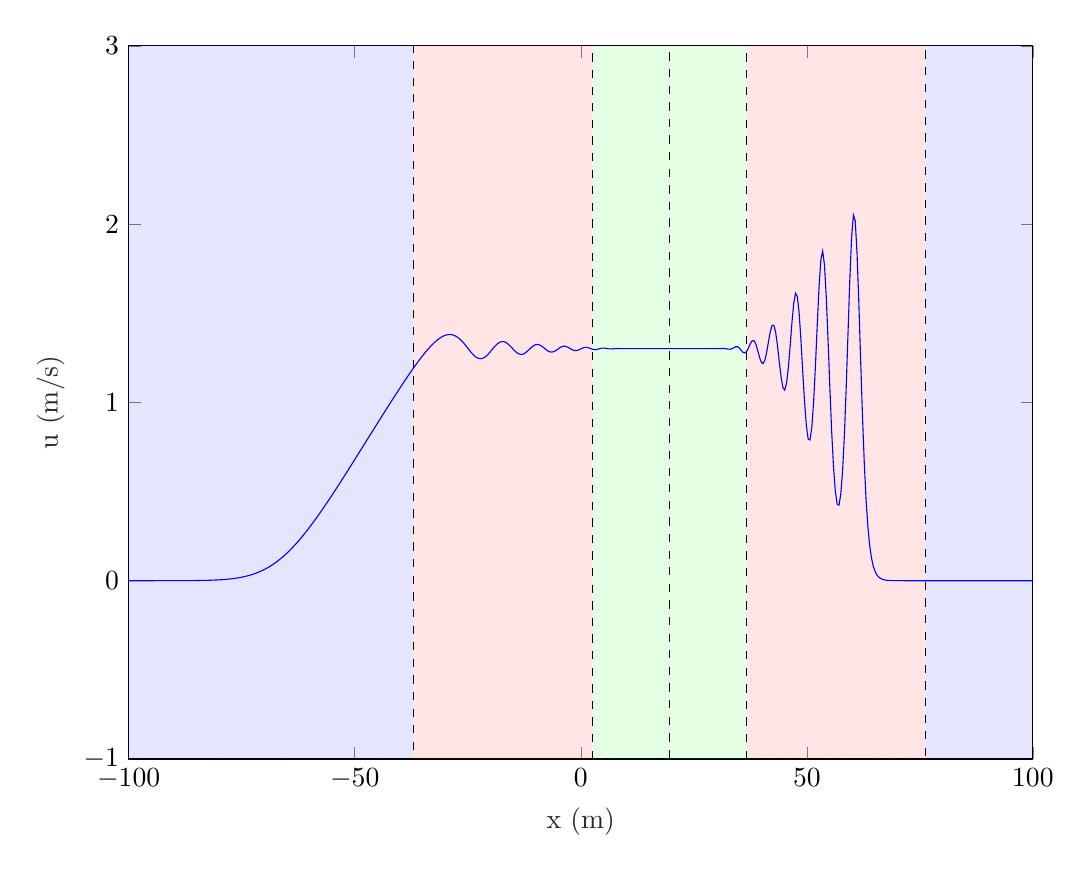
\begin{tikzpicture}

\begin{axis}[%
width=4.521in,
height=3.566in,
at={(0.758in,0.481in)},
scale only axis,
xmin=-100,
xmax=100,
xtick={-100,  -50,    0,   50,  100},
xlabel style={font=\color{white!15!black}},
xlabel={x (m)},
ymin=-1,
ymax=3,
ytick={-1,  0,  1,  2,  3},
ylabel style={font=\color{white!15!black}},
ylabel={u (m/s)},
axis background/.style={fill=white}
]

\addplot[area legend, dashed, draw=black, fill=blue, fill opacity=0.1, forget plot]
table[row sep=crcr] {%
x	y\\
-100	-1\\
-100	3\\
-37.0630892039997	3\\
-37.0630892039997	-1\\
}--cycle;

\addplot[area legend, draw=none, fill=red, fill opacity=0.1, forget plot]
table[row sep=crcr] {%
x	y\\
-37.0630892039997	-1\\
-37.0630892039997	3\\
2.50779195864934	3\\
2.50779195864934	-1\\
}--cycle;

\addplot[area legend, dashed, draw=black, fill=green, fill opacity=0.1, forget plot]
table[row sep=crcr] {%
x	y\\
2.50779195864934	-1\\
2.50779195864934	3\\
19.5890566189392	3\\
19.5890566189392	-1\\
}--cycle;

\addplot[area legend, draw=none, fill=green, fill opacity=0.1, forget plot]
table[row sep=crcr] {%
x	y\\
19.5890566189392	-1\\
19.5890566189392	3\\
36.670321279229	3\\
36.670321279229	-1\\
}--cycle;

\addplot[area legend, dashed, draw=black, fill=red, fill opacity=0.1, forget plot]
table[row sep=crcr] {%
x	y\\
36.670321279229	-1\\
36.670321279229	3\\
76.2412024418781	3\\
76.2412024418781	-1\\
}--cycle;

\addplot[area legend, draw=none, fill=blue, fill opacity=0.1, forget plot]
table[row sep=crcr] {%
x	y\\
76.2412024418781	-1\\
76.2412024418781	3\\
100	3\\
100	-1\\
}--cycle;
\addplot [color=blue, forget plot]
  table[row sep=crcr]{%
-100.1200120012	0\\
-99.7199719971997	4.68412773485595e-07\\
-99.3199319931993	1.37247843545677e-06\\
-98.9198919891989	2.48718810795974e-06\\
-98.5198519851985	3.71709056458455e-06\\
-98.1198119811981	5.0578960148718e-06\\
-97.7197719771977	6.53352371129432e-06\\
-97.3197319731973	8.17836074814186e-06\\
-96.9196919691969	1.00327273267152e-05\\
-96.5196519651965	1.21422236344367e-05\\
-96.1196119611961	1.45582617537928e-05\\
-95.7195719571957	1.7339014604035e-05\\
-95.3195319531953	2.0550573442334e-05\\
-94.9194919491949	2.42682680150664e-05\\
-94.5194519451945	2.8578151098829e-05\\
-94.1194119411941	3.35786641830883e-05\\
-93.7193719371937	3.93825065013952e-05\\
-93.3193319331933	4.61187326614538e-05\\
-92.9192919291929	5.39351064755654e-05\\
-92.5192519251925	6.30007407703027e-05\\
-92.1192119211921	7.35090552011226e-05\\
-91.7191719171917	8.56810864339899e-05\\
-91.3191319131913	9.97691873224593e-05\\
-90.9190919091909	0.000116061153870619\\
-90.5190519051905	0.00013488482108408\\
-90.1190119011901	0.000156613170707015\\
-89.7189718971897	0.000181669995669223\\
-89.3189318931893	0.000210536167480482\\
-88.9188918891889	0.000243756553899118\\
-88.5188518851885	0.000281947634632185\\
-88.1188118811881	0.000325805862635792\\
-87.7187718771877	0.000376116817544396\\
-87.3187318731873	0.000433765195838519\\
-86.9186918691869	0.000499745678957205\\
-86.5186518651865	0.000575174716245426\\
-86.1186118611861	0.00066130325324951\\
-85.7185718571857	0.000759530428149878\\
-85.3185318531853	0.000871418249078836\\
-84.9184918491849	0.000998707252927205\\
-84.5184518451845	0.00114333313174252\\
-84.1184118411841	0.0013074442955309\\
-83.7183718371837	0.00149342032039078\\
-83.3183318331833	0.00170389120797996\\
-82.9182918291829	0.00194175735642305\\
-82.5182518251825	0.00221021011401864\\
-82.1182118211821	0.00251275275524416\\
-81.7181718171817	0.00285322168408536\\
-81.3181318131813	0.00323580763284081\\
-80.9180918091809	0.00366507658556165\\
-80.5180518051805	0.00414599011490661\\
-80.1180118011801	0.00468392478026442\\
-79.7179717971797	0.00528469019407829\\
-79.3179317931793	0.00595454532402785\\
-78.9178917891789	0.00670021256193781\\
-78.5178517851785	0.00752888905763564\\
-78.1178117811781	0.00844825478925236\\
-77.7177717771777	0.00946647682204123\\
-77.3177317731773	0.010592209197936\\
-76.9176917691769	0.0118345878992879\\
-76.5176517651765	0.0132032203447146\\
-76.1176117611761	0.0147081689041465\\
-75.7175717571757	0.0163599279657299\\
-75.3175317531753	0.0181693941503675\\
-74.9174917491749	0.0201478293511891\\
-74.5174517451745	0.0223068163752896\\
-74.1174117411741	0.0246582070835565\\
-73.7173717371737	0.0272140630600156\\
-73.3173317331733	0.0299865889932467\\
-72.9172917291729	0.0329880591162092\\
-72.5172517251725	0.0362307372239754\\
-72.1172117211721	0.0397267909668885\\
-71.7171717171717	0.0434882012948624\\
-71.3171317131713	0.0475266681008586\\
-70.9170917091709	0.0518535132725638\\
-70.5170517051705	0.0564795825041191\\
-70.1170117011701	0.0614151473389204\\
-69.7169716971697	0.0666698090034807\\
-69.3169316931693	0.0722524056466562\\
-68.9168916891689	0.0781709246133505\\
-68.5168516851685	0.0844324213544707\\
-68.1168116811681	0.0910429465036308\\
-67.7167716771677	0.0980074825357763\\
-67.3167316731673	0.105329891265737\\
-66.9166916691669	0.113012873248277\\
-66.5166516651665	0.12105793991161\\
-66.1166116611661	0.129465398999222\\
-65.7165716571657	0.138234353618752\\
-65.3165316531653	0.147362714909762\\
-64.9164916491649	0.156847228054087\\
-64.5164516451645	0.16668351107242\\
-64.1164116411641	0.176866105587614\\
-63.7163716371637	0.18738853849755\\
-63.3163316331633	0.198243393295419\\
-62.9162916291629	0.209422389608582\\
-62.5162516251625	0.220916469403205\\
-62.1162116211621	0.232715888222999\\
-61.7161716171617	0.244810309797214\\
-61.3161316131613	0.257188902364303\\
-60.9160916091609	0.269840435111065\\
-60.5160516051605	0.282753373217818\\
-60.1160116011601	0.295915970123582\\
-59.7159715971597	0.309316355774934\\
-59.3159315931593	0.322942619791568\\
-58.9158915891589	0.336782888664037\\
-58.5158515851585	0.350825396287886\\
-58.1158115811581	0.365058547327154\\
-57.7157715771577	0.379470973083526\\
-57.3157315731573	0.39405157972026\\
-56.9156915691569	0.408789588848316\\
-56.5156515651565	0.423674570623188\\
-56.1156115611561	0.438696469622337\\
-55.7155715571557	0.453845623873754\\
-55.3155315531553	0.469112777485977\\
-54.9154915491549	0.484489087388755\\
-54.5154515451545	0.499966124733006\\
-54.1154115411541	0.515535871519883\\
-53.7153715371537	0.531190713033736\\
-53.3153315331533	0.546923426644324\\
-52.9152915291529	0.562727167522583\\
-52.5152515251525	0.578595451782958\\
-52.1152115211521	0.594522137526784\\
-51.7151715171517	0.610501404216773\\
-51.3151315131513	0.626527730764596\\
-50.9150915091509	0.642595872663343\\
-50.5150515051505	0.658700838445456\\
-50.1150115011501	0.674837865695856\\
-49.7149714971497	0.691002396800531\\
-49.3149314931493	0.707190054562768\\
-48.9148914891489	0.723396617773503\\
-48.5148514851485	0.739617996779022\\
-48.1148114811481	0.755850209048227\\
-47.7147714771477	0.772089354702862\\
-47.3147314731473	0.788331591937393\\
-46.9146914691469	0.804573112219881\\
-46.5146514651465	0.820810115131087\\
-46.1146114611461	0.837038782665068\\
-45.7145714571457	0.853255252780503\\
-45.3145314531453	0.869455591956849\\
-44.9144914491449	0.885635766472527\\
-44.5144514451445	0.901791612082534\\
-44.1144114411441	0.91791880172971\\
-43.7143714371437	0.934012810875466\\
-43.3143314331433	0.950068879982289\\
-42.9142914291429	0.966081973619282\\
-42.5142514251425	0.982046735593169\\
-42.1142114211421	0.997957439428816\\
-41.7141714171417	1.01380793343437\\
-41.3141314131413	1.02959157948521\\
-40.9140914091409	1.04530118454692\\
-40.5140514051405	1.06092892382975\\
-40.1140114011401	1.07646625432409\\
-39.7139713971397	1.09190381730991\\
-39.3139313931393	1.10723132826175\\
-38.9138913891389	1.1224374523889\\
-38.5138513851385	1.1375096638611\\
-38.1138113811381	1.15243408658086\\
-37.7137713771377	1.16719531418591\\
-37.3137313731373	1.18177620681652\\
-36.9136913691369	1.19615766208733\\
-36.5136513651365	1.21031835769817\\
-36.1136113611361	1.22423446325345\\
-35.7135713571357	1.23787931920548\\
-35.3135313531353	1.25122308148774\\
-34.9134913491349	1.2642323314885\\
-34.5134513451345	1.2768696527015\\
-34.1134113411341	1.28909317789704\\
-33.7133713371337	1.30085611426358\\
-33.3133313331333	1.3121062590208\\
-32.9132913291329	1.32278552491709\\
-32.5132513251325	1.33282950427563\\
-32.1132113211321	1.34216711236148\\
-31.7131713171317	1.35072036631113\\
-31.3131313131313	1.35840437508622\\
-30.9130913091309	1.3651276389997\\
-30.5130513051305	1.37079278390053\\
-30.1130113011301	1.37529788378234\\
-29.7129712971297	1.37853855370699\\
-29.3129312931293	1.38041101782543\\
-28.9128912891289	1.38081625689807\\
-28.5128512851285	1.37966580529772\\
-28.1128112811281	1.37688915659442\\
-27.7127712771277	1.37244217255344\\
-27.3127312731273	1.36631747849469\\
-26.9126912691269	1.35855586290237\\
-26.5126512651265	1.34925805565385\\
-26.1126112611261	1.33859580427516\\
-25.7125712571257	1.32682072966997\\
-25.3125312531253	1.31426908755534\\
-24.9124912491249	1.30136039079828\\
-24.5124512451245	1.28858796714889\\
-24.1124112411241	1.27650006458188\\
-23.7123712371237	1.26567111537332\\
-23.3123312331233	1.25666417775363\\
-22.9122912291229	1.24998720304816\\
-22.5122512251225	1.24604732808286\\
-22.1122112211221	1.2451086807253\\
-21.7121712171217	1.24725840191381\\
-21.3121312131213	1.25238699849485\\
-20.9120912091209	1.26018575694135\\
-20.5120512051205	1.27016166422743\\
-20.1120112011201	1.28166876017552\\
-19.7119711971197	1.29395232044901\\
-19.3119311931193	1.30620112443208\\
-18.9118911891189	1.31760289710766\\
-18.5118511851185	1.32739867988791\\
-18.1118111811181	1.33493308771037\\
-17.7117711771177	1.33969863470331\\
-17.3117311731173	1.34137299640519\\
-16.9116911691169	1.33984864415659\\
-16.5116511651165	1.33525311808765\\
-16.1116111611161	1.32795637144905\\
-15.7115711571157	1.31856249139174\\
-15.3115311531153	1.30788055291395\\
-14.9114911491149	1.29687116608228\\
-14.5114511451145	1.28656789621085\\
-14.1114111411141	1.27797730396792\\
-13.7113711371137	1.27196689534467\\
-13.3113311331133	1.26915549584177\\
-12.9112911291129	1.26982393536304\\
-12.5112511251125	1.27386082183792\\
-12.1112111211121	1.28076006507283\\
-11.7111711171117	1.28966969198303\\
-11.3111311131113	1.29948965261881\\
-10.9110911091109	1.30900527647665\\
-10.5110511051105	1.31703869929459\\
-10.1110111011101	1.32259910331438\\
-9.71097109710971	1.32501393671879\\
-9.3109310931093	1.32402496571538\\
-8.9108910891089	1.31983829668322\\
-8.51085108510851	1.31311367307405\\
-8.11081108110811	1.30489154025627\\
-7.71077107710771	1.29645556020156\\
-7.31073107310731	1.28914239967344\\
-6.9106910691069	1.28412306624998\\
-6.5106510651065	1.28219256545388\\
-6.11061106110611	1.28361126634907\\
-5.71057105710571	1.28803560486523\\
-5.31053105310531	1.29456638588425\\
-4.91049104910491	1.30190796756266\\
-4.5104510451045	1.30861547581189\\
-4.1104110411041	1.31338176868808\\
-3.71037103710371	1.31530739143077\\
-3.31033103310331	1.3140962072948\\
-2.91029102910291	1.31013582528022\\
-2.51025102510251	1.30442626922922\\
-2.1102110211021	1.29836817429694\\
-1.7101710171017	1.29343689730297\\
-1.31013101310131	1.29081412328536\\
-0.91009100910091	1.29107092753114\\
-0.510051005100507	1.29399659908867\\
-0.110011001100105	1.29864504193282\\
0.290029002900297	1.30359713769875\\
0.6900690069007	1.30737960666846\\
1.09010901090109	1.30891798015085\\
1.49014901490149	1.30788207706966\\
1.89018901890189	1.30480065152189\\
2.2902290229023	1.30088657218108\\
2.6902690269027	1.29760714322719\\
3.0903090309031	1.29613286415784\\
3.4903490349035	1.29687427552319\\
3.89038903890389	1.29931027829567\\
4.29042904290429	1.30222418296808\\
4.6904690469047	1.30426680531686\\
5.0905090509051	1.3046053473558\\
5.4905490549055	1.30332809386742\\
5.8905890589059	1.30137757399143\\
6.29062906290629	1.2999712122473\\
6.69066906690669	1.29981001976305\\
7.0907090709071	1.30064554093175\\
7.4907490749075	1.30162955288993\\
7.8907890789079	1.30209694399377\\
8.2908290829083	1.30199457597497\\
8.69086908690869	1.3016660529589\\
9.09090909090909	1.30143124500781\\
9.4909490949095	1.30138059959882\\
9.8909890989099	1.30144156823333\\
10.2910291029103	1.30151825122214\\
10.6910691069107	1.30156369356391\\
11.0911091109111	1.30157780757114\\
11.4911491149115	1.30157763791628\\
11.8911891189119	1.30157670014501\\
12.2912291229123	1.30157982741266\\
12.6912691269127	1.30158620342394\\
13.0913091309131	1.30159408844029\\
13.4913491349135	1.30160212502394\\
13.8913891389139	1.30160961343852\\
14.2914291429143	1.30161651537535\\
14.6914691469147	1.30162303619743\\
15.0915091509151	1.30162929705145\\
15.4915491549155	1.30163550828075\\
15.8915891589159	1.30164164022514\\
16.2916291629163	1.30164750882124\\
16.6916691669167	1.30165316846911\\
17.0917091709171	1.30165862261158\\
17.4917491749175	1.30166396495487\\
17.8917891789179	1.30166926786143\\
18.2918291829183	1.30167448733504\\
18.6918691869187	1.30167947871844\\
19.0919091909191	1.3016842780988\\
19.4919491949195	1.3016889411019\\
19.8919891989199	1.30169358372238\\
20.2920292029203	1.30169821588644\\
20.6920692069207	1.30170282657166\\
21.0921092109211	1.30170730241029\\
21.4921492149215	1.30171163030384\\
21.8921892189219	1.30171585921746\\
22.2922292229223	1.30172011294026\\
22.6922692269227	1.30172438779996\\
23.0923092309231	1.30172863003308\\
23.4923492349235	1.30173276140855\\
23.8923892389239	1.30173683250118\\
24.2924292429243	1.30174082037614\\
24.6924692469247	1.30174465509302\\
25.0925092509251	1.30174844145343\\
25.4925492549255	1.30175210733098\\
25.8925892589259	1.30175575166909\\
26.2926292629263	1.30175965707234\\
26.6926692669267	1.30176448765178\\
27.0927092709271	1.30177088189834\\
27.4927492749275	1.30177865227525\\
27.8927892789279	1.30178502818834\\
28.2928292829283	1.30178338781938\\
28.6928692869287	1.30176467763857\\
29.0929092909291	1.30172564165541\\
29.4929492949295	1.30168404542045\\
29.8929892989299	1.30169279907209\\
30.2930293029303	1.30183019704713\\
30.6930693069307	1.30213753912393\\
31.0931093109311	1.30249908603034\\
31.4931493149315	1.30255739011945\\
31.8931893189319	1.30184140562053\\
32.2932293229323	1.30021442563035\\
32.6932693269327	1.29847117740396\\
33.0933093309331	1.29836964603925\\
33.4933493349335	1.30147112642188\\
33.8933893389339	1.30726152006068\\
34.2934293429343	1.31228026762559\\
34.6934693469347	1.31198522900717\\
35.0935093509351	1.30426361116351\\
35.4935493549355	1.29164340589198\\
35.8935893589359	1.28041780529064\\
36.2936293629363	1.27745571749143\\
36.6936693669367	1.28657002992246\\
37.0937093709371	1.30614597796746\\
37.4937493749375	1.32912105334437\\
37.8937893789379	1.3454669389191\\
38.2938293829383	1.34632773777442\\
38.6938693869387	1.32811813302406\\
39.0939093909391	1.29468982318982\\
39.4939493949395	1.25640625792702\\
39.8939893989399	1.22667902787915\\
40.2940294029403	1.21749437290796\\
40.6940694069407	1.23536211755274\\
41.0941094109411	1.27874900184517\\
41.4941494149415	1.33750392213804\\
41.8941894189419	1.39484399514765\\
42.2942294229423	1.43176384564197\\
42.6942694269427	1.43312617410486\\
43.0943094309431	1.39342327816997\\
43.4943494349435	1.31949583549009\\
43.8943894389439	1.22848194254197\\
44.2944294429443	1.14268191440042\\
44.6944694469447	1.08390227760586\\
45.0945094509451	1.06882597765427\\
45.4945494549455	1.1057329801387\\
45.8945894589459	1.19223544705504\\
46.2946294629463	1.31411245474963\\
46.6946694669467	1.44615737970041\\
47.0947094709471	1.55615542640247\\
47.4947494749475	1.61233641448181\\
47.8947894789479	1.59367347606805\\
48.2948294829483	1.49893353381903\\
48.6948694869487	1.34732872972848\\
49.0949094909491	1.17011504784052\\
49.4949494949495	1.00086848636041\\
49.8949894989499	0.868466205467505\\
50.2950295029503	0.793751046657598\\
50.6950695069507	0.789348169637287\\
51.0951095109511	0.860403798891176\\
51.4951495149515	1.00364833825605\\
51.8951895189519	1.20427713786717\\
52.2952295229523	1.43319471206607\\
52.6952695269527	1.64831501105893\\
53.0953095309531	1.80112036199291\\
53.4953495349535	1.848656311459\\
53.8953895389539	1.77224600065709\\
54.2954295429543	1.58965935930659\\
54.6954695469547	1.34238727295095\\
55.0955095509551	1.07695293431955\\
55.4955495549555	0.833046928448585\\
55.8955895589559	0.637037045974456\\
56.2956295629563	0.501530823093168\\
56.6956695669567	0.430113313410933\\
57.0957095709571	0.423441515081933\\
57.4957495749575	0.483336846412263\\
57.8957895789579	0.613249756172731\\
58.2958295829583	0.814591334312622\\
58.6958695869587	1.07957484244156\\
59.0959095909591	1.38390286627199\\
59.4959495949595	1.6848086558738\\
59.8959895989599	1.92661455456517\\
60.2960296029603	2.05093848540876\\
60.6960696069607	2.0181377860041\\
61.0961096109611	1.83738451405362\\
61.4961496149615	1.55817071298402\\
61.8961896189619	1.23833239429758\\
62.2962296229623	0.928342465124194\\
62.6962696269627	0.662262430339468\\
63.0963096309631	0.4542418939567\\
63.4963496349635	0.302615443404253\\
63.8963896389639	0.197513704473797\\
64.2964296429643	0.127141911816238\\
64.6964696469647	0.0811014285844856\\
65.0965096509651	0.0514310401693928\\
65.4965496549655	0.0324947061566694\\
65.8965896589659	0.0204831754105933\\
66.2966296629663	0.0128934556622805\\
66.6966696669667	0.00810919681348401\\
67.0967096709671	0.00509778532119119\\
67.4967496749675	0.00320392053343107\\
67.8967896789679	0.00201346202352024\\
68.2968296829683	0.00126534477574194\\
68.6968696869687	0.000795254214032088\\
69.0969096909691	0.000499866254215874\\
69.4969496949695	0.000314243277397318\\
69.8969896989699	0.000197584464941753\\
70.2970297029703	0.000124257482268772\\
70.6970697069707	7.81596313081878e-05\\
71.0971097109711	4.91744328778411e-05\\
71.4971497149715	3.09456529695849e-05\\
71.8971897189719	1.94791479756449e-05\\
72.2972297229723	1.22647039486067e-05\\
72.6972697269727	7.72445947263809e-06\\
73.0973097309731	4.86643078091393e-06\\
73.4973497349735	3.06684891852827e-06\\
73.8973897389739	1.93340148643675e-06\\
74.2974297429743	1.21929428632127e-06\\
74.6974697469747	7.69239196846929e-07\\
75.0975097509751	4.85501738459292e-07\\
75.4975497549755	3.06554320855204e-07\\
75.8975897589759	1.93652335283137e-07\\
76.2976297629763	1.22390774561849e-07\\
76.6976697669767	7.73923311378429e-08\\
77.0977097709771	4.89647761800673e-08\\
77.4977497749775	3.09970330922059e-08\\
77.8977897789779	1.96345762939353e-08\\
78.2978297829783	1.24452360230294e-08\\
78.6978697869787	7.89369904490869e-09\\
79.0979097909791	5.01037121745315e-09\\
79.4979497949795	3.18264459368139e-09\\
79.8979897989799	2.02325966122635e-09\\
80.2980298029803	1.28729165504003e-09\\
80.6980698069807	8.19751553638374e-10\\
81.0981098109811	5.22498148473994e-10\\
81.4981498149815	3.33349035021214e-10\\
81.8981898189819	2.1288137066891e-10\\
82.2982298229823	1.36089084390964e-10\\
82.6982698269827	8.70890478324335e-11\\
83.0983098309831	5.57904310158635e-11\\
83.4983498349835	3.57808047762124e-11\\
83.8983898389839	2.29743334580155e-11\\
84.2984298429843	1.47680293892932e-11\\
84.6984698469847	9.49949756673477e-12\\
85.0985098509851	6.11435273683539e-12\\
85.4985498549855	3.93549483733004e-12\\
85.8985898589859	2.53291946891736e-12\\
86.2986298629863	1.62583256079169e-12\\
86.6986698669867	1.03984202782766e-12\\
87.0987098709871	6.60297857450699e-13\\
87.4987498749875	4.14572022392173e-13\\
87.8987898789879	2.55540569087628e-13\\
88.2988298829883	1.54003747551986e-13\\
88.6988698869887	8.77041146775042e-14\\
89.0989098909891	4.71957786415408e-14\\
89.4989498949895	2.39401854080217e-14\\
89.8989898989899	1.23659181591046e-14\\
90.2990299029903	6.38741635920806e-15\\
90.6990699069907	3.29931730268155e-15\\
91.0991099109911	1.70420934719254e-15\\
91.4991499149915	8.80281959148632e-16\\
91.8991899189919	4.54695503740873e-16\\
92.2992299229923	2.34865657500453e-16\\
92.6992699269927	1.21316082121673e-16\\
93.0993099309931	6.2663873199034e-17\\
93.4993499349935	3.23680169577997e-17\\
93.8993899389939	1.67191791276012e-17\\
94.2994299429943	8.63602333528157e-18\\
94.6994699469947	4.46079903456115e-18\\
95.0995099509951	2.30415392799812e-18\\
95.4995499549955	1.19017340756806e-18\\
95.8995899589959	6.1476439850684e-19\\
96.2996299629963	3.1754560032937e-19\\
96.6996699669967	1.64021000669888e-19\\
97.0997099709971	8.4718390566966e-20\\
97.4997499749975	4.37521366271506e-20\\
97.8997899789979	2.25843878455453e-20\\
98.2998299829983	1.1636416970228e-20\\
98.6998699869987	5.9541011958589e-21\\
99.0999099909991	2.96610648387117e-21\\
99.4999499949995	1.32031992553695e-21\\
99.8999899989999	2.719981511285e-22\\
};
\end{axis}
\end{tikzpicture}%
		\caption{$u$}
	\end{subfigure}
	\caption{Solution of gSGN with $\beta_1 = \beta_2 = \dfrac{1}{15}$ (Serre equations with improved dispersion charachteristics) for smooth dam-break problem at $t=15s$ with inequality regions shown.}
	\label{fig:SerreSDBImpDisp}
\end{figure}

\begin{figure}
	\tikzset{every picture/.style={scale=0.75}}%
	\centering
	\begin{subfigure}{0.49\textwidth}
		\centering
		% This file was created by matlab2tikz.
%
%The latest updates can be retrieved from
%  http://www.mathworks.com/matlabcentral/fileexchange/22022-matlab2tikz-matlab2tikz
%where you can also make suggestions and rate matlab2tikz.
%
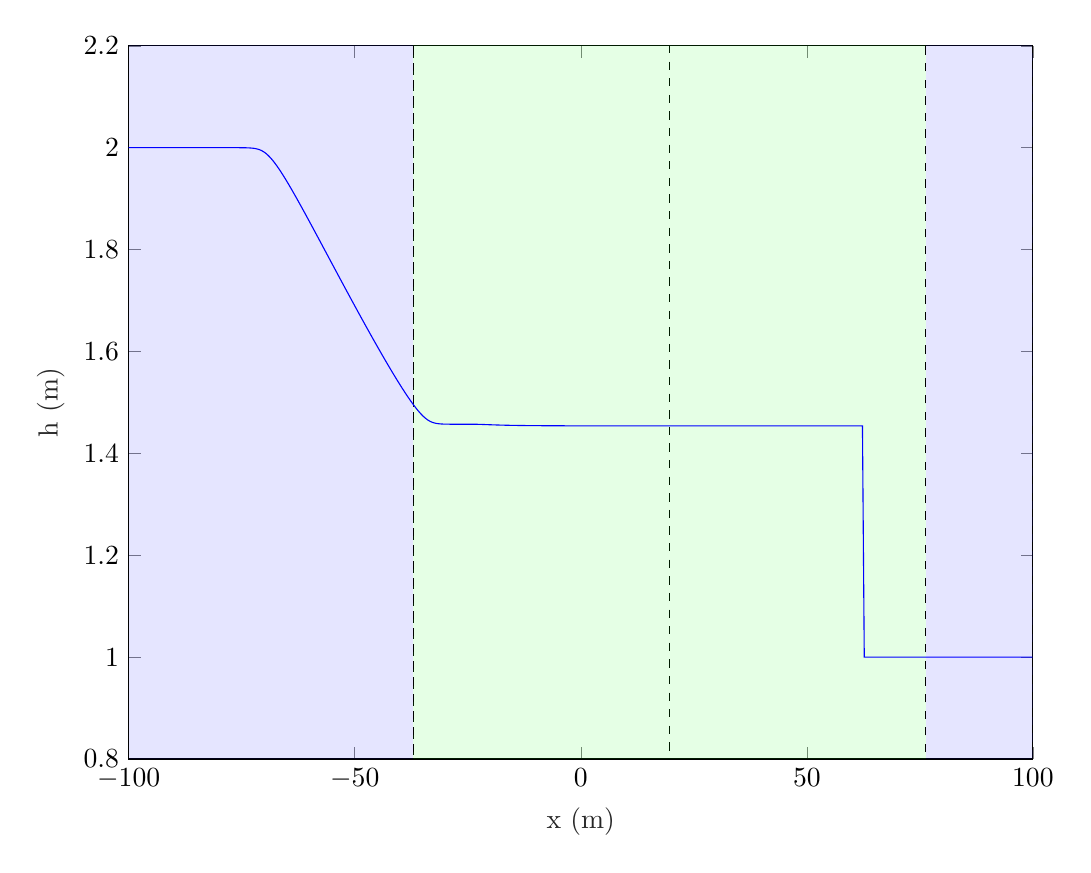
\begin{tikzpicture}

\begin{axis}[%
width=4.521in,
height=3.566in,
at={(0.758in,0.481in)},
scale only axis,
xmin=-100,
xmax=100,
xtick={-100,  -50,    0,   50,  100},
xlabel style={font=\color{white!15!black}},
xlabel={x (m)},
ymin=0.8,
ymax=2.2,
ytick={0.8,   1, 1.2, 1.4, 1.6, 1.8,   2, 2.2},
ylabel style={font=\color{white!15!black}},
ylabel={h (m)},
axis background/.style={fill=white}
]

\addplot[area legend, dashed, draw=black, fill=blue, fill opacity=0.1, forget plot]
table[row sep=crcr] {%
x	y\\
-100	-3\\
-100	3\\
-37.0630892039997	3\\
-37.0630892039997	-3\\
}--cycle;

\addplot[area legend, dashed, draw=black, fill=green, fill opacity=0.1, forget plot]
table[row sep=crcr] {%
x	y\\
-37.0630892039997	-3\\
-37.0630892039997	3\\
19.5890566189392	3\\
19.5890566189392	-3\\
}--cycle;

\addplot[area legend, draw=none, fill=green, fill opacity=0.1, forget plot]
table[row sep=crcr] {%
x	y\\
19.5890566189392	-3\\
19.5890566189392	3\\
76.2412024418781	3\\
76.2412024418781	-3\\
}--cycle;

\addplot[area legend, dashed, draw=black, fill=blue, fill opacity=0.1, forget plot]
table[row sep=crcr] {%
x	y\\
76.2412024418781	-3\\
76.2412024418781	3\\
100	3\\
100	-3\\
}--cycle;
\addplot [color=blue, forget plot]
  table[row sep=crcr]{%
-100.1200120012	2\\
-99.7199719971997	2\\
-99.3199319931993	2\\
-98.9198919891989	2\\
-98.5198519851985	2\\
-98.1198119811981	1.99999999999999\\
-97.7197719771977	1.99999999999999\\
-97.3197319731973	1.99999999999998\\
-96.9196919691969	1.99999999999997\\
-96.5196519651965	1.99999999999996\\
-96.1196119611961	1.99999999999994\\
-95.7195719571957	1.9999999999999\\
-95.3195319531953	1.99999999999985\\
-94.9194919491949	1.99999999999978\\
-94.5194519451945	1.99999999999968\\
-94.1194119411941	1.99999999999952\\
-93.7193719371937	1.99999999999928\\
-93.3193319331933	1.99999999999893\\
-92.9192919291929	1.99999999999841\\
-92.5192519251925	1.99999999999763\\
-92.1192119211921	1.99999999999645\\
-91.7191719171917	1.99999999999471\\
-91.3191319131913	1.99999999999211\\
-90.9190919091909	1.99999999998823\\
-90.5190519051905	1.99999999998244\\
-90.1190119011901	1.99999999997381\\
-89.7189718971897	1.99999999996092\\
-89.3189318931893	1.9999999999417\\
-88.9188918891889	1.99999999991303\\
-88.5188518851885	1.99999999987024\\
-88.1188118811881	1.99999999980642\\
-87.7187718771877	1.9999999997112\\
-87.3187318731873	1.99999999956914\\
-86.9186918691869	1.99999999935721\\
-86.5186518651865	1.99999999904103\\
-86.1186118611861	1.99999999856934\\
-85.7185718571857	1.99999999786562\\
-85.3185318531853	1.99999999681579\\
-84.9184918491849	1.99999999524965\\
-84.5184518451845	1.99999999291306\\
-84.1184118411841	1.99999998942711\\
-83.7183718371837	1.99999998422649\\
-83.3183318331833	1.99999997646775\\
-82.9182918291829	1.99999996489263\\
-82.5182518251825	1.99999994762391\\
-82.1182118211821	1.99999992186103\\
-81.7181718171817	1.99999988342592\\
-81.3181318131813	1.99999982608546\\
-80.9180918091809	1.99999974054077\\
-80.5180518051805	1.99999961291938\\
-80.1180118011801	1.99999942252614\\
-79.7179717971797	1.99999913848839\\
-79.3179317931793	1.99999871475237\\
-78.9178917891789	1.99999808262162\\
-78.5178517851785	1.99999713963222\\
-78.1178117811781	1.99999573297147\\
-77.7177717771777	1.9999936347754\\
-77.3177317731773	1.99999050535289\\
-76.9176917691769	1.99998583849213\\
-76.5176517651765	1.9999788802457\\
-76.1176117611761	1.99996850861262\\
-75.7175717571757	1.9999530559069\\
-75.3175317531753	1.9999300478715\\
-74.9174917491749	1.99989582350247\\
-74.5174517451745	1.99984498754921\\
-74.1174117411741	1.99976963611015\\
-73.7173717371737	1.99965829123995\\
-73.3173317331733	1.9994944977959\\
-72.9172917291729	1.99925510274861\\
-72.5172517251725	1.99890839587262\\
-72.1172117211721	1.99841257989026\\
-71.7171717171717	1.99771543194572\\
-71.3171317131713	1.99675631385204\\
-70.9170917091709	1.9954714453554\\
-70.5170517051705	1.99380215687772\\
-70.1170117011701	1.99170398312082\\
-69.7169716971697	1.98915330613979\\
-69.3169316931693	1.98614911632147\\
-68.9168916891689	1.98270988524878\\
-68.5168516851685	1.97886760275343\\
-68.1168116811681	1.97466143931244\\
-67.7167716771677	1.970132627673\\
-67.3167316731673	1.96532106420588\\
-66.9166916691669	1.96026343632199\\
-66.5166516651665	1.95499243781459\\
-66.1166116611661	1.94953665224664\\
-65.7165716571657	1.94392079435739\\
-65.3165316531653	1.93816611124749\\
-64.9164916491649	1.93229082911311\\
-64.5164516451645	1.92631058596417\\
-64.1164116411641	1.92023882323649\\
-63.7163716371637	1.91408712715289\\
-63.3163316331633	1.90786551988031\\
-62.9162916291629	1.90158270475123\\
-62.5162516251625	1.8952462713604\\
-62.1162116211621	1.88886286653179\\
-61.7161716171617	1.882438336706\\
-61.3161316131613	1.87597784661229\\
-60.9160916091609	1.86948597835872\\
-60.5160516051605	1.86296681438864\\
-60.1160116011601	1.85642400714998\\
-59.7159715971597	1.84986083781204\\
-59.3159315931593	1.84328026593763\\
-58.9158915891589	1.83668497166575\\
-58.5158515851585	1.83007739168943\\
-58.1158115811581	1.82345975010046\\
-57.7157715771577	1.81683408490893\\
-57.3157315731573	1.81020227075615\\
-56.9156915691569	1.80356603842666\\
-56.5156515651565	1.79692699228495\\
-56.1156115611561	1.79028662653726\\
-55.7155715571557	1.78364633952335\\
-55.3155315531553	1.77700744441394\\
-54.9154915491549	1.77037117724541\\
-54.5154515451545	1.76373870593444\\
-54.1154115411541	1.75711114130609\\
-53.7153715371537	1.75048954629397\\
-53.3153315331533	1.74387494115666\\
-52.9152915291529	1.73726830892092\\
-52.5152515251525	1.73067060420532\\
-52.1152115211521	1.724082760421\\
-51.7151715171517	1.71750569088851\\
-51.3151315131513	1.7109402903255\\
-50.9150915091509	1.70438744413148\\
-50.5150515051505	1.69784803921488\\
-50.1150115011501	1.69132296651589\\
-49.7149714971497	1.68481312018075\\
-49.3149314931493	1.67831940398103\\
-48.9148914891489	1.67184274159523\\
-48.5148514851485	1.66538408175274\\
-48.1148114811481	1.6589444012307\\
-47.7147714771477	1.65252471231067\\
-47.3147314731473	1.64612607190842\\
-46.9146914691469	1.63974958878497\\
-46.5146514651465	1.63339643165518\\
-46.1146114611461	1.62706783972849\\
-45.7145714571457	1.62076513407345\\
-45.3145314531453	1.61448973023413\\
-44.9144914491449	1.60824315305664\\
-44.5144514451445	1.60202705334846\\
-44.1144114411441	1.59584322702655\\
-43.7143714371437	1.58969363788087\\
-43.3143314331433	1.5835804442028\\
-42.9142914291429	1.57750602986162\\
-42.5142514251425	1.57147304074887\\
-42.1142114211421	1.56548442799472\\
-41.7141714171417	1.55954350043702\\
-41.3141314131413	1.55365398743191\\
-40.9140914091409	1.54782011308323\\
-40.5140514051405	1.54204668711773\\
-40.1140114011401	1.53633921627671\\
-39.7139713971397	1.53070403821826\\
-39.3139313931393	1.52514848596463\\
-38.9138913891389	1.51968108987095\\
-38.5138513851385	1.5143118230641\\
-38.1138113811381	1.50905240132486\\
-37.7137713771377	1.50391664422503\\
-37.3137313731373	1.49892090323306\\
-36.9136913691369	1.49408455351931\\
-36.5136513651365	1.48943052640473\\
-36.1136113611361	1.48498582243197\\
-35.7135713571357	1.48078187209598\\
-35.3135313531353	1.47685449630941\\
-34.9134913491349	1.47324304798179\\
-34.5134513451345	1.46998813572408\\
-34.1134113411341	1.46712730387127\\
-33.7133713371337	1.46468846189344\\
-33.3133313331333	1.46268207617707\\
-32.9132913291329	1.46109488711964\\
-32.5132513251325	1.45988875506157\\
-32.1132113211321	1.4590064235308\\
-31.7131713171317	1.45838208792976\\
-31.3131313131313	1.45795208117124\\
-30.9130913091309	1.45766194981287\\
-30.5130513051305	1.4574690933303\\
-30.1130113011301	1.45734222710925\\
-29.7129712971297	1.45725936162267\\
-29.3129312931293	1.45720549334089\\
-28.9128912891289	1.45717058633626\\
-28.5128512851285	1.4571480147833\\
-28.1128112811281	1.45713344150874\\
-27.7127712771277	1.45712404316205\\
-27.3127312731273	1.45711798826324\\
-26.9126912691269	1.4571140910178\\
-26.5126512651265	1.45711158362441\\
-26.1126112611261	1.45710996649685\\
-25.7125712571257	1.4571089075897\\
-25.3125312531253	1.45710816803852\\
-24.9124912491249	1.457107528681\\
-24.5124512451245	1.45710667099653\\
-24.1124112411241	1.45710486490965\\
-23.7123712371237	1.45710371215055\\
-23.3123312331233	1.45708072099705\\
-22.9122912291229	1.45699829445062\\
-22.5122512251225	1.45688959815283\\
-22.1122112211221	1.45677154074113\\
-21.7121712171217	1.45664491464926\\
-21.3121312131213	1.45651209686004\\
-20.9120912091209	1.4563762336698\\
-20.5120512051205	1.4562407158822\\
-20.1120112011201	1.4561076279883\\
-19.7119711971197	1.45597877122568\\
-19.3119311931193	1.45585564261276\\
-18.9118911891189	1.45573720326185\\
-18.5118511851185	1.45562469045578\\
-18.1118111811181	1.45551798493277\\
-17.7117711771177	1.45541740851169\\
-17.3117311731173	1.45532220343416\\
-16.9116911691169	1.45523238301776\\
-16.5116511651165	1.4551483705928\\
-16.1116111611161	1.45506884135665\\
-15.7115711571157	1.45499439414156\\
-15.3115311531153	1.45492438644256\\
-14.9114911491149	1.45485883434411\\
-14.5114511451145	1.45479722268867\\
-14.1114111411141	1.45473959405182\\
-13.7113711371137	1.45468562407338\\
-13.3113311331133	1.45463457952365\\
-12.9112911291129	1.45458704545768\\
-12.5112511251125	1.4545424604751\\
-12.1112111211121	1.45450062418416\\
-11.7111711171117	1.45446124443453\\
-11.3111311131113	1.45442448998106\\
-10.9110911091109	1.45438978910506\\
-10.5110511051105	1.45435757732522\\
-10.1110111011101	1.4543270349334\\
-9.71097109710971	1.45429860890565\\
-9.3109310931093	1.45427176571406\\
-8.9108910891089	1.45424662988252\\
-8.51085108510851	1.45422300079641\\
-8.11081108110811	1.45420080182472\\
-7.71077107710771	1.45417995087287\\
-7.31073107310731	1.45416037136018\\
-6.9106910691069	1.45414196043788\\
-6.5106510651065	1.45412466336458\\
-6.11061106110611	1.45410841177001\\
-5.71057105710571	1.45409317557675\\
-5.31053105310531	1.45407883047077\\
-4.91049104910491	1.45406519912513\\
-4.5104510451045	1.45405242271871\\
-4.1104110411041	1.4540405511109\\
-3.71037103710371	1.45402937138347\\
-3.31033103310331	1.4540184427968\\
-2.91029102910291	1.45400874627722\\
-2.51025102510251	1.45399937814984\\
-2.1102110211021	1.45399014353623\\
-1.7101710171017	1.45398214465648\\
-1.31013101310131	1.45397416262774\\
-0.91009100910091	1.45396670640899\\
-0.510051005100507	1.45395988386057\\
-0.110011001100105	1.45395296335125\\
0.290029002900297	1.4539471381016\\
0.6900690069007	1.45394089510847\\
1.09010901090109	1.45393577553495\\
1.49014901490149	1.45393018509531\\
1.89018901890189	1.45392563361382\\
2.2902290229023	1.45392060830841\\
2.6902690269027	1.45391662368743\\
3.0903090309031	1.45391204387055\\
3.4903490349035	1.45390856583632\\
3.89038903890389	1.45390452992925\\
4.29042904290429	1.45390131408687\\
4.6904690469047	1.45389785838778\\
5.0905090509051	1.45389469949931\\
5.4905490549055	1.45389211922005\\
5.8905890589059	1.45388906286769\\
6.29062906290629	1.45388671240873\\
6.69066906690669	1.45388404329426\\
7.0907090709071	1.45388180457463\\
7.4907490749075	1.45387956148363\\
7.8907890789079	1.45387716577817\\
8.2908290829083	1.45387552627158\\
8.69086908690869	1.45387340735488\\
9.09090909090909	1.45387182618569\\
9.4909490949095	1.45387034107157\\
9.8909890989099	1.45386857697808\\
10.2910291029103	1.45386715776617\\
10.6910691069107	1.45386580132301\\
11.0911091109111	1.45386411495782\\
11.4911491149115	1.45386315892391\\
11.8911891189119	1.45386219897224\\
12.2912291229123	1.45386095960166\\
12.6912691269127	1.45386011193179\\
13.0913091309131	1.45385907288651\\
13.4913491349135	1.45385781735207\\
13.8913891389139	1.45385709876387\\
14.2914291429143	1.45385643395316\\
14.6914691469147	1.45385553986828\\
15.0915091509151	1.45385486131625\\
15.4915491549155	1.45385405113379\\
15.8915891589159	1.4538531956454\\
16.2916291629163	1.45385270044113\\
16.6916691669167	1.45385218416127\\
17.0917091709171	1.45385153769841\\
17.4917491749175	1.45385083538883\\
17.8917891789179	1.45385043790226\\
18.2918291829183	1.45384988663998\\
18.6918691869187	1.45384948500253\\
19.0919091909191	1.453849085778\\
19.4919491949195	1.45384857833137\\
19.8919891989199	1.45384804398457\\
20.2920292029203	1.45384788344571\\
20.6920692069207	1.45384751022594\\
21.0921092109211	1.45384707426193\\
21.4921492149215	1.45384666912596\\
21.8921892189219	1.45384648688642\\
22.2922292229223	1.45384624617877\\
22.6922692269227	1.45384592999559\\
23.0923092309231	1.4538456928901\\
23.4923492349235	1.45384535373373\\
23.8923892389239	1.45384507554413\\
24.2924292429243	1.45384504069344\\
24.6924692469247	1.45384479425439\\
25.0925092509251	1.45384444870269\\
25.4925492549255	1.45384425976184\\
25.8925892589259	1.45384432041659\\
26.2926292629263	1.45384406814095\\
26.6926692669267	1.45384372856975\\
27.0927092709271	1.45384357438173\\
27.4927492749275	1.45384363797942\\
27.8927892789279	1.45384347709787\\
28.2928292829283	1.45384319715112\\
28.6928692869287	1.4538430620842\\
29.0929092909291	1.45384310510292\\
29.4929492949295	1.45384296346383\\
29.8929892989299	1.45384280192386\\
30.2930293029303	1.45384271484652\\
30.6930693069307	1.45384260646391\\
31.0931093109311	1.45384260850224\\
31.4931493149315	1.45384254734809\\
31.8931893189319	1.4538423159154\\
32.2932293229323	1.45384214620777\\
32.6932693269327	1.45384232004519\\
33.0933093309331	1.45384229706708\\
33.4933493349335	1.45384199601712\\
33.8933893389339	1.45384185997374\\
34.2934293429343	1.4538421306342\\
34.6934693469347	1.45384211382159\\
35.0935093509351	1.45384173623127\\
35.4935493549355	1.45384162846269\\
35.8935893589359	1.45384191934021\\
36.2936293629363	1.45384189611905\\
36.6936693669367	1.45384154110284\\
37.0937093709371	1.45384146287123\\
37.4937493749375	1.45384173531721\\
37.8937893789379	1.45384172720275\\
38.2938293829383	1.45384141243441\\
38.6938693869387	1.45384134099888\\
39.0939093909391	1.45384158479125\\
39.4939493949395	1.45384155797275\\
39.8939893989399	1.45384133245515\\
40.2940294029403	1.45384128883434\\
40.6940694069407	1.45384142267247\\
41.0941094109411	1.45384139594244\\
41.4941494149415	1.45384132562301\\
41.8941894189419	1.45384125209301\\
42.2942294229423	1.45384122301705\\
42.6942694269427	1.45384134345942\\
43.0943094309431	1.45384140577262\\
43.4943494349435	1.4538410934293\\
43.8943894389439	1.45384102191432\\
44.2944294429443	1.45384132220724\\
44.6944694469447	1.45384143353312\\
45.0945094509451	1.45384096141764\\
45.4945494549455	1.45384092192721\\
45.8945894589459	1.45384132111373\\
46.2946294629463	1.45384144054848\\
46.6946694669467	1.45384086150238\\
47.0947094709471	1.45384086453025\\
47.4947494749475	1.45384138393006\\
47.8947894789479	1.45384138878154\\
48.2948294829483	1.45384078591114\\
48.6948694869487	1.4538408062737\\
49.0949094909491	1.45384142023876\\
49.4949494949495	1.45384125091577\\
49.8949894989499	1.45384077977479\\
50.2950295029503	1.4538407033293\\
50.6950695069507	1.45384149762261\\
51.0951095109511	1.45384103754554\\
51.4951495149515	1.4538409031074\\
51.8951895189519	1.45384046245381\\
52.2952295229523	1.45384174887457\\
52.6952695269527	1.45384066621454\\
53.0953095309531	1.45384130750493\\
53.4953495349535	1.4538399846453\\
53.8953895389539	1.45384225595284\\
54.2954295429543	1.45383988248501\\
54.6954695469547	1.45384227628999\\
55.0955095509551	1.45383890753286\\
55.4955495549555	1.4538434023746\\
55.8955895589559	1.45383837477877\\
56.2956295629563	1.45384433081865\\
56.6956695669567	1.45383656783735\\
57.0957095709571	1.45384562775157\\
57.4957495749575	1.45383547088346\\
57.8957895789579	1.45384841769518\\
58.2958295829583	1.45383179515641\\
58.6958695869587	1.45385061405405\\
59.0959095909591	1.45382925917418\\
59.4959495949595	1.45385607967265\\
59.8959895989599	1.45382262123379\\
60.2960296029603	1.45386066778075\\
60.6960696069607	1.45381704652221\\
61.0961096109611	1.45386966597628\\
61.4961496149615	1.4538061088152\\
61.8961896189619	1.45387662285077\\
62.2962296229623	1.45379093546777\\
62.6962696269627	1.00012576995479\\
63.0963096309631	1.00000005035169\\
63.4963496349635	1.00000003375035\\
63.8963896389639	1.00000002262261\\
64.2964296429643	1.00000001516377\\
64.6964696469647	1.00000001016418\\
65.0965096509651	1.00000000681298\\
65.4965496549655	1.00000000456669\\
65.8965896589659	1.00000000306101\\
66.2966296629663	1.00000000205179\\
66.6966696669667	1.00000000137529\\
67.0967096709671	1.00000000092187\\
67.4967496749675	1.00000000061791\\
67.8967896789679	1.00000000041416\\
68.2968296829683	1.00000000027761\\
68.6968696869687	1.00000000018608\\
69.0969096909691	1.00000000012473\\
69.4969496949695	1.00000000008361\\
69.8969896989699	1.00000000005605\\
70.2970297029703	1.00000000003758\\
70.6970697069707	1.0000000000252\\
71.0971097109711	1.0000000000169\\
71.4971497149715	1.0000000000113\\
71.8971897189719	1.00000000000762\\
72.2972297229723	1.00000000000511\\
72.6972697269727	1.00000000000336\\
73.0973097309731	1.00000000000224\\
73.4973497349735	1.00000000000151\\
73.8973897389739	1.00000000000101\\
74.2974297429743	1.0000000000007\\
74.6974697469747	1.00000000000048\\
75.0975097509751	1.00000000000036\\
75.4975497549755	1.00000000000023\\
75.8975897589759	1.00000000000017\\
76.2976297629763	1.00000000000013\\
76.6976697669767	1.00000000000007\\
77.0977097709771	1.00000000000002\\
77.4977497749775	1\\
77.8977897789779	1\\
78.2978297829783	1\\
78.6978697869787	1\\
79.0979097909791	1\\
79.4979497949795	1\\
79.8979897989799	1\\
80.2980298029803	1\\
80.6980698069807	1\\
81.0981098109811	1\\
81.4981498149815	1\\
81.8981898189819	1\\
82.2982298229823	1\\
82.6982698269827	1\\
83.0983098309831	1\\
83.4983498349835	1\\
83.8983898389839	1\\
84.2984298429843	1\\
84.6984698469847	1\\
85.0985098509851	1\\
85.4985498549855	1\\
85.8985898589859	1\\
86.2986298629863	1\\
86.6986698669867	1\\
87.0987098709871	1\\
87.4987498749875	1\\
87.8987898789879	1\\
88.2988298829883	1\\
88.6988698869887	1\\
89.0989098909891	1\\
89.4989498949895	1\\
89.8989898989899	1\\
90.2990299029903	1\\
90.6990699069907	1\\
91.0991099109911	1\\
91.4991499149915	1\\
91.8991899189919	1\\
92.2992299229923	1\\
92.6992699269927	1\\
93.0993099309931	1\\
93.4993499349935	1\\
93.8993899389939	1\\
94.2994299429943	1\\
94.6994699469947	1\\
95.0995099509951	1\\
95.4995499549955	1\\
95.8995899589959	1\\
96.2996299629963	1\\
96.6996699669967	1\\
97.0997099709971	1\\
97.4997499749975	1\\
97.8997899789979	1\\
98.2998299829983	1\\
98.6998699869987	1\\
99.0999099909991	1\\
99.4999499949995	1\\
99.8999899989999	1\\
};
\end{axis}
\end{tikzpicture}%
		\caption{$h$}
	\end{subfigure}
	\begin{subfigure}{0.49\textwidth}
		\centering
		% This file was created by matlab2tikz.
%
%The latest updates can be retrieved from
%  http://www.mathworks.com/matlabcentral/fileexchange/22022-matlab2tikz-matlab2tikz
%where you can also make suggestions and rate matlab2tikz.
%
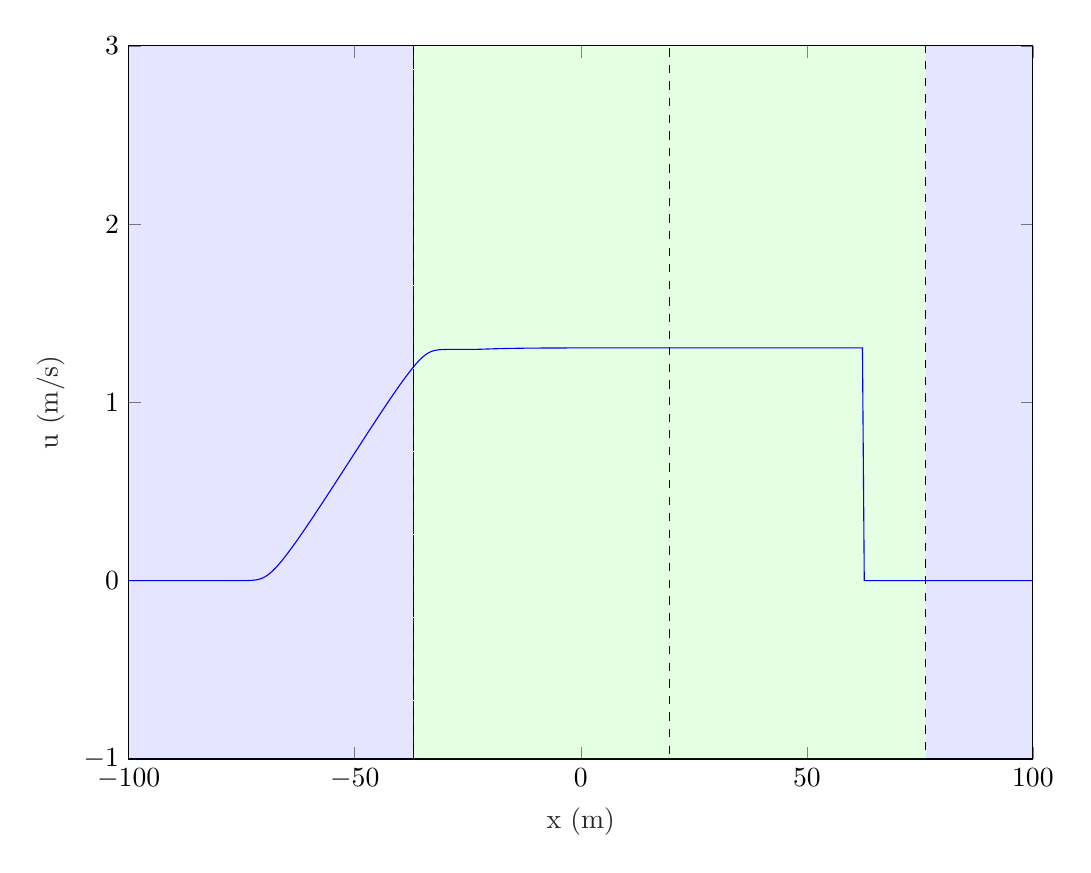
\begin{tikzpicture}

\begin{axis}[%
width=4.521in,
height=3.566in,
at={(0.758in,0.481in)},
scale only axis,
xmin=-100,
xmax=100,
xtick={-100,  -50,    0,   50,  100},
xlabel style={font=\color{white!15!black}},
xlabel={x (m)},
ymin=-1,
ymax=3,
ytick={-1,  0,  1,  2,  3},
ylabel style={font=\color{white!15!black}},
ylabel={u (m/s)},
axis background/.style={fill=white}
]

\addplot[area legend, dashed, draw=black, fill=blue, fill opacity=0.1, forget plot]
table[row sep=crcr] {%
x	y\\
-100	-3\\
-100	3\\
-37.0630892039997	3\\
-37.0630892039997	-3\\
}--cycle;

\addplot[area legend, dashed, draw=black, fill=green, fill opacity=0.1, forget plot]
table[row sep=crcr] {%
x	y\\
-37.0630892039997	-3\\
-37.0630892039997	3\\
19.5890566189392	3\\
19.5890566189392	-3\\
}--cycle;

\addplot[area legend, draw=none, fill=green, fill opacity=0.1, forget plot]
table[row sep=crcr] {%
x	y\\
19.5890566189392	-3\\
19.5890566189392	3\\
76.2412024418781	3\\
76.2412024418781	-3\\
}--cycle;

\addplot[area legend, dashed, draw=black, fill=blue, fill opacity=0.1, forget plot]
table[row sep=crcr] {%
x	y\\
76.2412024418781	-3\\
76.2412024418781	3\\
100	3\\
100	-3\\
}--cycle;
\addplot [color=blue, forget plot]
  table[row sep=crcr]{%
-100.1200120012	0\\
-99.7199719971997	1.20310066172386e-15\\
-99.3199319931993	1.20310066172386e-15\\
-98.9198919891989	1.20310066172386e-15\\
-98.5198519851985	4.01033553907953e-15\\
-98.1198119811981	1.26325569481006e-14\\
-97.7197719771977	2.13550367455986e-14\\
-97.3197319731973	3.85994795636408e-14\\
-96.9196919691969	6.17591673018257e-14\\
-96.5196519651965	9.74511535996348e-14\\
-96.1196119611961	1.35749857997846e-13\\
-95.7195719571957	2.18362770102891e-13\\
-95.3195319531953	3.22631494118972e-13\\
-94.9194919491949	4.79034580143102e-13\\
-94.5194519451945	7.1424075951018e-13\\
-94.1194119411941	1.06434305207196e-12\\
-93.7193719371937	1.58558641376414e-12\\
-93.3193319331933	2.35988194797261e-12\\
-92.9192919291929	3.51886891876813e-12\\
-92.5192519251925	5.25975557628601e-12\\
-92.1192119211921	7.8533398278049e-12\\
-91.7191719171917	1.17064702137695e-11\\
-91.3191319131913	1.74745358196656e-11\\
-90.9190919091909	2.60646745444584e-11\\
-90.5190519051905	3.88802030517174e-11\\
-90.1190119011901	5.80086012480489e-11\\
-89.7189718971897	8.6539030599488e-11\\
-89.3189318931893	1.29104732013351e-10\\
-88.9188918891889	1.92611703806107e-10\\
-88.5188518851885	2.87357384802956e-10\\
-88.1188118811881	4.28703866585211e-10\\
-87.7187718771877	6.39581245196873e-10\\
-87.3187318731873	9.54182644062348e-10\\
-86.9186918691869	1.42352805327816e-09\\
-86.5186518651865	2.12373674955616e-09\\
-86.1186118611861	3.16836589569138e-09\\
-85.7185718571857	4.72682680368017e-09\\
-85.3185318531853	7.05179607999013e-09\\
-84.9184918491849	1.05201874203771e-08\\
-84.5184518451845	1.56948281670943e-08\\
-84.1184118411841	2.34148462627066e-08\\
-83.7183718371837	3.49322089550453e-08\\
-83.3183318331833	5.21148211584671e-08\\
-82.9182918291829	7.77492299605816e-08\\
-82.5182518251825	1.15992747197557e-07\\
-82.1182118211821	1.73047553814648e-07\\
-81.7181718171817	2.581664368374e-07\\
-81.3181318131813	3.85153335609719e-07\\
-80.9180918091809	5.74601711342825e-07\\
-80.5180518051805	8.57233696637947e-07\\
-80.1180118011801	1.27888103023171e-06\\
-79.7179717971797	1.90791476353846e-06\\
-79.3179317931793	2.84632620362215e-06\\
-78.9178917891789	4.24625156482475e-06\\
-78.5178517851785	6.33460918633692e-06\\
-78.1178117811781	9.44982089550209e-06\\
-77.7177717771777	1.40965190991419e-05\\
-77.3177317731773	2.10269925014753e-05\\
-76.9176917691769	3.13623140245558e-05\\
-76.5176517651765	4.67722070155116e-05\\
-76.1176117611761	6.9741517600241e-05\\
-75.7175717571757	0.000103963631895029\\
-75.3175317531753	0.000154918309112971\\
-74.9174917491749	0.000230713781119599\\
-74.5174517451745	0.000343299596139778\\
-74.1174117411741	0.000510182368859854\\
-73.7173717371737	0.000756786804900984\\
-73.3173317331733	0.00111956648080909\\
-72.9172917291729	0.00164982131205373\\
-72.5172517251725	0.00241782853176445\\
-72.1172117211721	0.00351625535406051\\
-71.7171717171717	0.00506095058718152\\
-71.3171317131713	0.00718655629407767\\
-70.9170917091709	0.0100349115555877\\
-70.5170517051705	0.0137368587699572\\
-70.1170117011701	0.0183921576435123\\
-69.7169716971697	0.024054765915593\\
-69.3169316931693	0.0307288634802072\\
-68.9168916891689	0.0383756546573989\\
-68.5168516851685	0.0469264410789162\\
-68.1168116811681	0.0562965466373097\\
-67.7167716771677	0.0663965792756074\\
-67.3167316731673	0.0771399202324\\
-66.9166916691669	0.0884468608222327\\
-66.5166516651665	0.100246346979299\\
-66.1166116611661	0.112476253321195\\
-65.7165716571657	0.125082867878753\\
-65.3165316531653	0.138020023322745\\
-64.9164916491649	0.151248126011885\\
-64.5164516451645	0.16473321407373\\
-64.1164116411641	0.178446104339091\\
-63.7163716371637	0.192361648476996\\
-63.3163316331633	0.206458098437861\\
-62.9162916291629	0.220716572000128\\
-62.5162516251625	0.235120605794511\\
-62.1162116211621	0.249655782749358\\
-61.7161716171617	0.264309421856854\\
-61.3161316131613	0.279070319649349\\
-60.9160916091609	0.293928534366848\\
-60.5160516051605	0.308875205290471\\
-60.1160116011601	0.323902401030126\\
-59.7159715971597	0.339002991670815\\
-59.3159315931593	0.354170540614654\\
-58.9158915891589	0.369399212725129\\
-58.5158515851585	0.384683695969387\\
-58.1158115811581	0.400019134215722\\
-57.7157715771577	0.415401069428963\\
-57.3157315731573	0.430825392159617\\
-56.9156915691569	0.446288299007442\\
-56.5156515651565	0.461786254507809\\
-56.1156115611561	0.477315955380278\\
-55.7155715571557	0.492874299028364\\
-55.3155315531553	0.508458360159185\\
-54.9154915491549	0.52406537343213\\
-54.5154515451545	0.539692713616919\\
-54.1154115411541	0.5553378707805\\
-53.7153715371537	0.570998429534588\\
-53.3153315331533	0.586672057512476\\
-52.9152915291529	0.602356493184321\\
-52.5152515251525	0.618049525486038\\
-52.1152115211521	0.633748977093646\\
-51.7151715171517	0.649452702062043\\
-51.3151315131513	0.66515858255626\\
-50.9150915091509	0.680864506832353\\
-50.5150515051505	0.696568343258946\\
-50.1150115011501	0.712267934056549\\
-49.7149714971497	0.72796109705572\\
-49.3149314931493	0.743645609952727\\
-48.9148914891489	0.759319185027259\\
-48.5148514851485	0.774979456054229\\
-48.1148114811481	0.790623970295332\\
-47.7147714771477	0.80625016953149\\
-47.3147314731473	0.821855366799539\\
-46.9146914691469	0.837436727569459\\
-46.5146514651465	0.852991248515498\\
-46.1146114611461	0.868515730081942\\
-45.7145714571457	0.884006746725078\\
-45.3145314531453	0.899460613748151\\
-44.9144914491449	0.91487334831991\\
-44.5144514451445	0.930240625542571\\
-44.1144114411441	0.945557727884106\\
-43.7143714371437	0.960819485097442\\
-43.3143314331433	0.976020203893531\\
-42.9142914291429	0.991153585795962\\
-42.5142514251425	1.00621263074525\\
-42.1142114211421	1.02118952278069\\
-41.7141714171417	1.03607549137923\\
-41.3141314131413	1.05086064544801\\
-40.9140914091409	1.0655337769765\\
-40.5140514051405	1.08008212085858\\
-40.1140114011401	1.09449106066237\\
-39.7139713971397	1.10874377478788\\
-39.3139313931393	1.12282080210799\\
-38.9138913891389	1.13669950868161\\
-38.5138513851385	1.1503534396329\\
-38.1138113811381	1.16375152743987\\
-37.7137713771377	1.17685713841157\\
-37.3137313731373	1.18962694208758\\
-36.9136913691369	1.20200961167313\\
-36.5136513651365	1.21394441526928\\
-36.1136113611361	1.22535985435855\\
-35.7135713571357	1.23617269670773\\
-35.3135313531353	1.24628805191909\\
-34.9134913491349	1.2556015850068\\
-34.5134513451345	1.26400543698337\\
-34.1134113411341	1.27139949563096\\
-33.7133713371337	1.2777085700091\\
-33.3133313331333	1.28290283848493\\
-32.9132913291329	1.2870143633742\\
-32.5132513251325	1.29014025134544\\
-32.1132113211321	1.29242775556672\\
-31.7131713171317	1.29404679181074\\
-31.3131313131313	1.2951620846585\\
-30.9130913091309	1.29591467604957\\
-30.5130513051305	1.29641497865511\\
-30.1130113011301	1.29674410821519\\
-29.7129712971297	1.29695909372152\\
-29.3129312931293	1.2970988521828\\
-28.9128912891289	1.29718941787276\\
-28.5128512851285	1.29724797995161\\
-28.1128112811281	1.29728579064746\\
-27.7127712771277	1.29731017495848\\
-27.3127312731273	1.29732588461647\\
-26.9126912691269	1.29733599616931\\
-26.5126512651265	1.29734250169265\\
-26.1126112611261	1.29734669737661\\
-25.7125712571257	1.29734944471939\\
-25.3125312531253	1.29735136344624\\
-24.9124912491249	1.29735302212976\\
-24.5124512451245	1.2973552470104\\
-24.1124112411241	1.29735993399805\\
-23.7123712371237	1.29736291431688\\
-23.3123312331233	1.2974225197586\\
-22.9122912291229	1.29763643330677\\
-22.5122512251225	1.2979185006304\\
-22.1122112211221	1.29822485669061\\
-21.7121712171217	1.29855346176069\\
-21.3121312131213	1.29889815015816\\
-20.9120912091209	1.29925075844605\\
-20.5120512051205	1.29960248573119\\
-20.1120112011201	1.29994792269806\\
-19.7119711971197	1.3002823913133\\
-19.3119311931193	1.30060200162737\\
-18.9118911891189	1.30090945888353\\
-18.5118511851185	1.30120153985293\\
-18.1118111811181	1.30147855656157\\
-17.7117711771177	1.30173966836207\\
-17.3117311731173	1.3019868468062\\
-16.9116911691169	1.30222005050906\\
-16.5116511651165	1.30243817879373\\
-16.1116111611161	1.30264467913955\\
-15.7115711571157	1.30283798491811\\
-15.3115311531153	1.30301976949735\\
-14.9114911491149	1.30318998685069\\
-14.5114511451145	1.30334997610034\\
-14.1114111411141	1.30349962230142\\
-13.7113711371137	1.30363977242428\\
-13.3113311331133	1.30377233343227\\
-12.9112911291129	1.30389577505745\\
-12.5112511251125	1.30401156009271\\
-12.1112111211121	1.30412020885993\\
-11.7111711171117	1.30422248158839\\
-11.3111311131113	1.30431793652427\\
-10.9110911091109	1.30440805985393\\
-10.5110511051105	1.30449171650979\\
-10.1110111011101	1.30457104071167\\
-9.71097109710971	1.30464486789461\\
-9.3109310931093	1.30471458671827\\
-8.9108910891089	1.30477987036077\\
-8.51085108510851	1.30484124131316\\
-8.11081108110811	1.30489889841681\\
-7.71077107710771	1.30495305471611\\
-7.31073107310731	1.30500390903438\\
-6.9106910691069	1.30505172834054\\
-6.5106510651065	1.30509665526714\\
-6.11061106110611	1.30513886680985\\
-5.71057105710571	1.30517844085529\\
-5.31053105310531	1.30521570099188\\
-4.91049104910491	1.3052511069201\\
-4.5104510451045	1.3052842932094\\
-4.1104110411041	1.30531512896904\\
-3.71037103710371	1.3053441662328\\
-3.31033103310331	1.3053725551244\\
-2.91029102910291	1.30539773921867\\
-2.51025102510251	1.30542207216032\\
-2.1102110211021	1.30544606164796\\
-1.7101710171017	1.30546683651675\\
-1.31013101310131	1.30548756981708\\
-0.91009100910091	1.30550693748858\\
-0.510051005100507	1.30552465810747\\
-0.110011001100105	1.30554263686578\\
0.290029002900297	1.30555776523837\\
0.6900690069007	1.30557398476534\\
1.09010901090109	1.30558728008809\\
1.49014901490149	1.30560180427017\\
1.89018901890189	1.30561362430008\\
2.2902290229023	1.30562668107364\\
2.6902690269027	1.30563702806527\\
3.0903090309031	1.30564892817702\\
3.4903490349035	1.30565795880588\\
3.89038903890389	1.30566844505804\\
4.29042904290429	1.3056767959318\\
4.6904690469047	1.30568577345668\\
5.0905090509051	1.30569397816428\\
5.4905490549055	1.3057006770733\\
5.8905890589059	1.30570861919236\\
6.29062906290629	1.30571472107098\\
6.69066906690669	1.30572165738072\\
7.0907090709071	1.30572747228334\\
7.4907490749075	1.30573329942128\\
7.8907890789079	1.30573952637631\\
8.2908290829083	1.30574378169663\\
8.69086908690869	1.30574928820404\\
9.09090909090909	1.30575339229335\\
9.4909490949095	1.30575724618737\\
9.8909890989099	1.30576183190729\\
10.2910291029103	1.30576551797092\\
10.6910691069107	1.30576904164719\\
11.0911091109111	1.30577342908797\\
11.4911491149115	1.30577590673361\\
11.8911891189119	1.30577839787863\\
12.2912291229123	1.30578161824587\\
12.6912691269127	1.30578381760958\\
13.0913091309131	1.30578651899322\\
13.4913491349135	1.30578978356086\\
13.8913891389139	1.30579164794159\\
14.2914291429143	1.30579337301564\\
14.6914691469147	1.30579569597634\\
15.0915091509151	1.30579745752971\\
15.4915491549155	1.30579956371143\\
15.8915891589159	1.30580178795792\\
16.2916291629163	1.30580307093907\\
16.6916691669167	1.30580441122207\\
17.0917091709171	1.30580609196488\\
17.4917491749175	1.30580791791099\\
17.8917891789179	1.30580894965695\\
18.2918291829183	1.30581038180852\\
18.6918691869187	1.30581142243842\\
19.0919091909191	1.30581246031084\\
19.4919491949195	1.30581377946989\\
19.8919891989199	1.30581516987843\\
20.2920292029203	1.30581558074711\\
20.6920692069207	1.30581655289925\\
21.0921092109211	1.30581768590077\\
21.4921492149215	1.30581873907574\\
21.8921892189219	1.30581921028597\\
22.2922292229223	1.30581983569932\\
22.6922692269227	1.30582065772077\\
23.0923092309231	1.30582127373313\\
23.4923492349235	1.30582215476747\\
23.8923892389239	1.30582288151672\\
24.2924292429243	1.30582296523233\\
24.6924692469247	1.30582360540208\\
25.0925092509251	1.30582450622945\\
25.4925492549255	1.30582500260415\\
25.8925892589259	1.30582483573873\\
26.2926292629263	1.30582548984399\\
26.6926692669267	1.30582637634858\\
27.0927092709271	1.3058267825951\\
27.4927492749275	1.30582660777596\\
27.8927892789279	1.30582702648096\\
28.2928292829283	1.30582775672676\\
28.6928692869287	1.30582811001879\\
29.0929092909291	1.30582799207957\\
29.4929492949295	1.30582836192636\\
29.8929892989299	1.30582878197032\\
30.2930293029303	1.30582900779783\\
30.6930693069307	1.30582929148594\\
31.0931093109311	1.30582928069418\\
31.4931493149315	1.3058294416002\\
31.8931893189319	1.30583004602972\\
32.2932293229323	1.30583048534975\\
32.6932693269327	1.30583002764876\\
33.0933093309331	1.30583009035634\\
33.4933493349335	1.30583087756881\\
33.8933893389339	1.3058312291948\\
34.2934293429343	1.30583051814444\\
34.6934693469347	1.30583056432427\\
35.0935093509351	1.30583155210788\\
35.4935493549355	1.30583183070653\\
35.8935893589359	1.30583106618729\\
36.2936293629363	1.30583112855916\\
36.6936693669367	1.30583205817193\\
37.0937093709371	1.30583225899129\\
37.4937493749375	1.30583154387666\\
37.8937893789379	1.30583156734215\\
38.2938293829383	1.30583239158334\\
38.6938693869387	1.30583257471396\\
39.0939093909391	1.30583193506839\\
39.4939493949395	1.30583200687202\\
39.8939893989399	1.30583259704103\\
40.2940294029403	1.30583270865001\\
40.6940694069407	1.30583235733094\\
41.0941094109411	1.30583242850931\\
41.4941494149415	1.30583261026248\\
41.8941894189419	1.30583280236354\\
42.2942294229423	1.30583287847741\\
42.6942694269427	1.30583256115841\\
43.0943094309431	1.30583239865085\\
43.4943494349435	1.30583321686745\\
43.8943894389439	1.30583339996667\\
44.2944294429443	1.30583261284275\\
44.6944694469447	1.3058323219765\\
45.0945094509451	1.30583355919421\\
45.4945494549455	1.30583365930063\\
45.8945894589459	1.30583261079062\\
46.2946294629463	1.30583229206305\\
46.6946694669467	1.30583381695887\\
47.0947094709471	1.3058338063623\\
47.4947494749475	1.30583244106974\\
47.8947894789479	1.30583242595369\\
48.2948294829483	1.30583400982424\\
48.6948694869487	1.30583395415898\\
49.0949094909491	1.30583233432749\\
49.4949494949495	1.3058328023817\\
49.8949894989499	1.30583402441377\\
50.2950295029503	1.30583422829934\\
50.6950695069507	1.30583212098331\\
51.0951095109511	1.3058333794263\\
51.4951495149515	1.30583367507895\\
51.8951895189519	1.30583487379059\\
52.2952295229523	1.30583143723593\\
52.6952695269527	1.3058343745553\\
53.0953095309531	1.30583258310065\\
53.4953495349535	1.30583612439725\\
53.8953895389539	1.30583008303063\\
54.2954295429543	1.30583642746269\\
54.6954695469547	1.3058300536614\\
55.0955095509551	1.3058389415638\\
55.4955495549555	1.30582708789906\\
55.8955895589559	1.30584035074381\\
56.2956295629563	1.30582460395265\\
56.6956695669567	1.30584508291233\\
57.0957095709571	1.30582115280522\\
57.4957495749575	1.30584783370659\\
57.8957895789579	1.30581397604087\\
58.2958295829583	1.30585722342469\\
58.6958695869587	1.30580821688969\\
59.0959095909591	1.30586358369973\\
59.4959495949595	1.3057936967549\\
59.8959895989599	1.3058807033107\\
60.2960296029603	1.30578093808863\\
60.6960696069607	1.30589543610573\\
61.0961096109611	1.3057554739883\\
61.4961496149615	1.30592420376048\\
61.8961896189619	1.30573544324779\\
62.2962296229623	1.30596833368334\\
62.6962696269627	0.000332225261428372\\
63.0963096309631	1.57698244619973e-07\\
63.4963496349635	1.05703905494044e-07\\
63.8963896389639	7.08525549637964e-08\\
64.2964296429643	4.74919504983337e-08\\
64.6964696469647	3.1833543146939e-08\\
65.0965096509651	2.13378173222618e-08\\
65.4965496549655	1.43025674767e-08\\
65.8965896589659	9.58689791866647e-09\\
66.2966296629663	6.42606605826271e-09\\
66.6966696669667	4.3073205304687e-09\\
67.0967096709671	2.8872363064252e-09\\
67.4967496749675	1.93524165297519e-09\\
67.8967896789679	1.2971278404322e-09\\
68.2968296829683	8.69453276929635e-10\\
68.6968696869687	5.82798703581465e-10\\
69.0969096909691	3.90647737267702e-10\\
69.4969496949695	2.61858618691872e-10\\
69.8969896989699	1.75541209273858e-10\\
70.2970297029703	1.17701643674957e-10\\
70.6970697069707	7.89289677476568e-11\\
71.0971097109711	5.29457030158889e-11\\
71.4971497149715	3.53905093232577e-11\\
71.8971897189719	2.38565336671119e-11\\
72.2972297229723	1.60123674819664e-11\\
72.6972697269727	1.0519260506553e-11\\
73.0973097309731	7.01538021688458e-12\\
73.4973497349735	4.71535252684261e-12\\
73.8973897389739	3.16214957256102e-12\\
74.2974297429743	2.1952576740906e-12\\
74.6974697469747	1.5110443019302e-12\\
75.0975097509751	1.1329699189838e-12\\
75.4975497549755	7.3604695900364e-13\\
75.8975897589759	5.54880051025796e-13\\
76.2976297629763	4.02888334094727e-13\\
76.6976697669767	2.35757600503621e-13\\
77.0977097709771	6.8927642077928e-14\\
77.4977497749775	0\\
77.8977897789779	0\\
78.2978297829783	0\\
78.6978697869787	0\\
79.0979097909791	0\\
79.4979497949795	0\\
79.8979897989799	0\\
80.2980298029803	0\\
80.6980698069807	0\\
81.0981098109811	0\\
81.4981498149815	0\\
81.8981898189819	0\\
82.2982298229823	0\\
82.6982698269827	0\\
83.0983098309831	0\\
83.4983498349835	0\\
83.8983898389839	0\\
84.2984298429843	0\\
84.6984698469847	0\\
85.0985098509851	0\\
85.4985498549855	0\\
85.8985898589859	0\\
86.2986298629863	0\\
86.6986698669867	0\\
87.0987098709871	0\\
87.4987498749875	0\\
87.8987898789879	0\\
88.2988298829883	0\\
88.6988698869887	0\\
89.0989098909891	0\\
89.4989498949895	0\\
89.8989898989899	0\\
90.2990299029903	0\\
90.6990699069907	0\\
91.0991099109911	0\\
91.4991499149915	0\\
91.8991899189919	0\\
92.2992299229923	0\\
92.6992699269927	0\\
93.0993099309931	0\\
93.4993499349935	0\\
93.8993899389939	0\\
94.2994299429943	0\\
94.6994699469947	0\\
95.0995099509951	0\\
95.4995499549955	0\\
95.8995899589959	0\\
96.2996299629963	0\\
96.6996699669967	0\\
97.0997099709971	0\\
97.4997499749975	0\\
97.8997899789979	0\\
98.2998299829983	0\\
98.6998699869987	0\\
99.0999099909991	0\\
99.4999499949995	0\\
99.8999899989999	0\\
};
\end{axis}
\end{tikzpicture}%
		\caption{$u$}
	\end{subfigure}
	\caption{Solution of gSGN with $\beta_1 = -\dfrac{2}{3} $ and $\beta_2 = 0$ (Shallow Water Wave Equations) for smooth dam-break problem at $t=15s$ with inequality regions shown.}
	\label{fig:SWWESDB}
\end{figure}

\begin{figure}
	\tikzset{every picture/.style={scale=0.75}}%
	\centering
	\begin{subfigure}{0.49\textwidth}
		\centering
		% This file was created by matlab2tikz.
%
%The latest updates can be retrieved from
%  http://www.mathworks.com/matlabcentral/fileexchange/22022-matlab2tikz-matlab2tikz
%where you can also make suggestions and rate matlab2tikz.
%
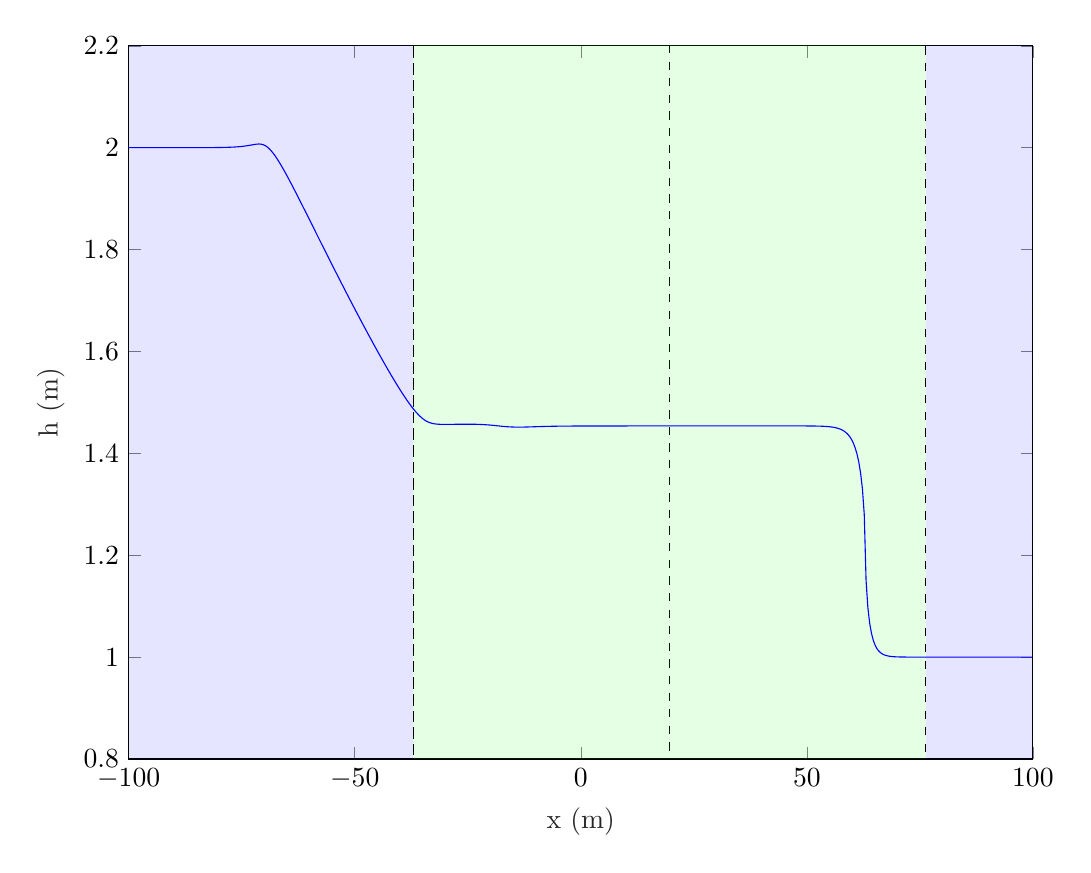
\begin{tikzpicture}

\begin{axis}[%
width=4.521in,
height=3.566in,
at={(0.758in,0.481in)},
scale only axis,
xmin=-100,
xmax=100,
xtick={-100,  -50,    0,   50,  100},
xlabel style={font=\color{white!15!black}},
xlabel={x (m)},
ymin=0.8,
ymax=2.2,
ytick={0.8,   1, 1.2, 1.4, 1.6, 1.8,   2, 2.2},
ylabel style={font=\color{white!15!black}},
ylabel={h (m)},
axis background/.style={fill=white}
]

\addplot[area legend, dashed, draw=black, fill=blue, fill opacity=0.1, forget plot]
table[row sep=crcr] {%
x	y\\
-100	-3\\
-100	3\\
-37.0630892039997	3\\
-37.0630892039997	-3\\
}--cycle;

\addplot[area legend, dashed, draw=black, fill=green, fill opacity=0.1, forget plot]
table[row sep=crcr] {%
x	y\\
-37.0630892039997	-3\\
-37.0630892039997	3\\
19.5890566189392	3\\
19.5890566189392	-3\\
}--cycle;

\addplot[area legend, draw=none, fill=green, fill opacity=0.1, forget plot]
table[row sep=crcr] {%
x	y\\
19.5890566189392	-3\\
19.5890566189392	3\\
76.2412024418781	3\\
76.2412024418781	-3\\
}--cycle;

\addplot[area legend, dashed, draw=black, fill=blue, fill opacity=0.1, forget plot]
table[row sep=crcr] {%
x	y\\
76.2412024418781	-3\\
76.2412024418781	3\\
100	3\\
100	-3\\
}--cycle;
\addplot [color=blue, forget plot]
  table[row sep=crcr]{%
-100.1200120012	2\\
-99.7199719971997	2.0000000435356\\
-99.3199319931993	2.00000009240499\\
-98.9198919891989	2.00000013657813\\
-98.5198519851985	2.00000017832431\\
-98.1198119811981	2.00000021968279\\
-97.7197719771977	2.0000002625423\\
-97.3197319731973	2.00000030871283\\
-96.9196919691969	2.00000035999204\\
-96.5196519651965	2.00000041822868\\
-96.1196119611961	2.00000048538494\\
-95.7195719571957	2.00000056359995\\
-95.3195319531953	2.00000065525636\\
-94.9194919491949	2.00000076305189\\
-94.5194519451945	2.00000089007823\\
-94.1194119411941	2.00000103990939\\
-93.7193719371937	2.0000012167021\\
-93.3193319331933	2.0000014253111\\
-92.9192919291929	2.00000167142236\\
-92.5192519251925	2.00000196170814\\
-92.1192119211921	2.00000230400785\\
-91.7191719171917	2.0000027075399\\
-91.3191319131913	2.00000318314992\\
-90.9190919091909	2.00000374360243\\
-90.5190519051905	2.00000440392348\\
-90.1190119011901	2.00000518180365\\
-89.7189718971897	2.0000060980722\\
-89.3189318931893	2.00000717725503\\
-88.9188918891889	2.00000844823147\\
-88.5188518851885	2.00000994500757\\
-88.1188118811881	2.0000117076264\\
-87.7187718771877	2.00001378323997\\
-87.3187318731873	2.00001622737116\\
-86.9186918691869	2.00001910539994\\
-86.5186518651865	2.00002249431321\\
-86.1186118611861	2.0000264847656\\
-85.7185718571857	2.00003118350567\\
-85.3185318531853	2.00003671623266\\
-84.9184918491849	2.00004323095981\\
-84.5184518451845	2.00005090197343\\
-84.1184118411841	2.0000599344927\\
-83.7183718371837	2.00007057015268\\
-83.3183318331833	2.00008309345393\\
-82.9182918291829	2.00009783934621\\
-82.5182518251825	2.00011520213765\\
-82.1182118211821	2.00013564595715\\
-81.7181718171817	2.00015971702251\\
-81.3181318131813	2.00018805800433\\
-80.9180918091809	2.00022142481503\\
-80.5180518051805	2.00026070617045\\
-80.1180118011801	2.00030694630407\\
-79.7179717971797	2.00036137120834\\
-79.3179317931793	2.00042541872524\\
-78.9178917891789	2.00050077274326\\
-78.5178517851785	2.00058940154479\\
-78.1178117811781	2.00069359976474\\
-77.7177717771777	2.00081603310955\\
-77.3177317731773	2.00095978315124\\
-76.9176917691769	2.00112838840692\\
-76.5176517651765	2.00132587377428\\
-76.1176117611761	2.00155675451011\\
-75.7175717571757	2.0018259947681\\
-75.3175317531753	2.00213888144925\\
-74.9174917491749	2.00250076154692\\
-74.5174517451745	2.00291653521809\\
-74.1174117411741	2.00338976801809\\
-73.7173717371737	2.00392120330472\\
-73.3173317331733	2.00450635700197\\
-72.9172917291729	2.00513185534618\\
-72.5172517251725	2.00577025496102\\
-72.1172117211721	2.0063736253379\\
-71.7171717171717	2.00686731827524\\
-71.3171317131713	2.00714645411996\\
-70.9170917091709	2.00707207628035\\
-70.5170517051705	2.00652147292071\\
-70.1170117011701	2.00537711819984\\
-69.7169716971697	2.0035673556492\\
-69.3169316931693	2.00107295606489\\
-68.9168916891689	1.9979202450105\\
-68.5168516851685	1.99416461560304\\
-68.1168116811681	1.98987504425053\\
-67.7167716771677	1.98512296491823\\
-67.3167316731673	1.97997583542566\\
-66.9166916691669	1.97449416838017\\
-66.5166516651665	1.96873065452799\\
-66.1166116611661	1.96273037129175\\
-65.7165716571657	1.95653151670493\\
-65.3165316531653	1.95016633553617\\
-64.9164916491649	1.94366198322545\\
-64.5164516451645	1.93704128727429\\
-64.1164116411641	1.93032347438458\\
-63.7163716371637	1.9235247876544\\
-63.3163316331633	1.91665895868676\\
-62.9162916291629	1.90973762254118\\
-62.5162516251625	1.90277067685542\\
-62.1162116211621	1.89576655999482\\
-61.7161716171617	1.88873248476353\\
-61.3161316131613	1.88167464238014\\
-60.9160916091609	1.87459835990538\\
-60.5160516051605	1.86750822987551\\
-60.1160116011601	1.86040823405418\\
-59.7159715971597	1.85330183255554\\
-59.3159315931593	1.84619204599775\\
-58.9158915891589	1.83908152034603\\
-58.5158515851585	1.83197258355905\\
-58.1158115811581	1.82486729282809\\
-57.7157715771577	1.81776747057521\\
-57.3157315731573	1.8106747456943\\
-56.9156915691569	1.80359058201044\\
-56.5156515651565	1.79651630060072\\
-56.1156115611561	1.78945309874437\\
-55.7155715571557	1.7824020707261\\
-55.3155315531553	1.77536422393335\\
-54.9154915491549	1.76834049265155\\
-54.5154515451545	1.76133175066228\\
-54.1154115411541	1.75433882008641\\
-53.7153715371537	1.74736248307102\\
-53.3153315331533	1.74040349332744\\
-52.9152915291529	1.73346257213993\\
-52.5152515251525	1.72654042163154\\
-52.1152115211521	1.71963773322086\\
-51.7151715171517	1.71275519640706\\
-51.3151315131513	1.7058935021294\\
-50.9150915091509	1.6990533427134\\
-50.5150515051505	1.69223542480577\\
-50.1150115011501	1.68544047853288\\
-49.7149714971497	1.67866925608745\\
-49.3149314931493	1.67192253885863\\
-48.9148914891489	1.66520114557441\\
-48.5148514851485	1.65850594064188\\
-48.1148114811481	1.6518378417097\\
-47.7147714771477	1.64519782854952\\
-47.3147314731473	1.63858695884296\\
-46.9146914691469	1.63200636170535\\
-46.5146514651465	1.62545726205277\\
-46.1146114611461	1.61894100067297\\
-45.7145714571457	1.61245904847956\\
-45.3145314531453	1.6060130161006\\
-44.9144914491449	1.59960469324634\\
-44.5144514451445	1.59323606673918\\
-44.1144114411441	1.58690934721694\\
-43.7143714371437	1.58062700954442\\
-43.3143314331433	1.57439183755402\\
-42.9142914291429	1.56820697239049\\
-42.5142514251425	1.56207597886077\\
-42.1142114211421	1.55600289944098\\
-41.7141714171417	1.54999234313066\\
-41.3141314131413	1.54404959814073\\
-40.9140914091409	1.53818073843087\\
-40.5140514051405	1.53239276160435\\
-40.1140114011401	1.52669376218163\\
-39.7139713971397	1.52109310338514\\
-39.3139313931393	1.51560163931476\\
-38.9138913891389	1.51023196344723\\
-38.5138513851385	1.50499867921017\\
-38.1138113811381	1.4999186941247\\
-37.7137713771377	1.4950114780384\\
-37.3137313731373	1.49029932683975\\
-36.9136913691369	1.48580749288909\\
-36.5136513651365	1.48156411785483\\
-36.1136113611361	1.47759980761893\\
-35.7135713571357	1.47394657425347\\
-35.3135313531353	1.47063604382358\\
-34.9134913491349	1.46769662385609\\
-34.5134513451345	1.46514967732937\\
-34.1134113411341	1.46300512911525\\
-33.7133713371337	1.46125758792356\\
-33.3133313331333	1.45988440508272\\
-32.9132913291329	1.45884696282193\\
-32.5132513251325	1.4580952931821\\
-32.1132113211321	1.45757458116109\\
-31.7131713171317	1.45723162442851\\
-31.3131313131313	1.45701946491657\\
-30.9130913091309	1.45689962684654\\
-30.5130513051305	1.45684237949725\\
-30.1130113011301	1.45682570497286\\
-29.7129712971297	1.45683340275302\\
-29.3129312931293	1.45685603165728\\
-28.9128912891289	1.45688633378074\\
-28.5128512851285	1.45691963574511\\
-28.1128112811281	1.45695313756001\\
-27.7127712771277	1.45698523056381\\
-27.3127312731273	1.45701508829652\\
-26.9126912691269	1.45704233928362\\
-26.5126512651265	1.45706683354598\\
-26.1126112611261	1.45708840084034\\
-25.7125712571257	1.45710654490133\\
-25.3125312531253	1.45712010221097\\
-24.9124912491249	1.45712766744074\\
-24.5124512451245	1.4571266806995\\
-24.1124112411241	1.45711116556131\\
-23.7123712371237	1.45707560013492\\
-23.3123312331233	1.45701439916946\\
-22.9122912291229	1.45692121556242\\
-22.5122512251225	1.45679188972416\\
-22.1122112211221	1.45663119471336\\
-21.7121712171217	1.4564471614676\\
-21.3121312131213	1.45624701692816\\
-20.9120912091209	1.45603738205934\\
-20.5120512051205	1.4557998628707\\
-20.1120112011201	1.4555180600995\\
-19.7119711971197	1.45519723354248\\
-19.3119311931193	1.45484683780576\\
-18.9118911891189	1.45447815921699\\
-18.5118511851185	1.45409898328521\\
-18.1118111811181	1.45371748927959\\
-17.7117711771177	1.45334376516773\\
-17.3117311731173	1.45298720608564\\
-16.9116911691169	1.45265578389761\\
-16.5116511651165	1.45236387412868\\
-16.1116111611161	1.45211690291352\\
-15.7115711571157	1.45190917165478\\
-15.3115311531153	1.45173739369731\\
-14.9114911491149	1.45160207942335\\
-14.5114511451145	1.45150568503203\\
-14.1114111411141	1.45144839858057\\
-13.7113711371137	1.45142721848226\\
-13.3113311331133	1.45143825066342\\
-12.9112911291129	1.45148311012774\\
-12.5112511251125	1.4515513517708\\
-12.1112111211121	1.45163911392919\\
-11.7111711171117	1.45174107966301\\
-11.3111311131113	1.45185233784725\\
-10.9110911091109	1.45196932180784\\
-10.5110511051105	1.4520887254703\\
-10.1110111011101	1.45220787155515\\
-9.71097109710971	1.45232509828404\\
-9.3109310931093	1.45243839185498\\
-8.9108910891089	1.4525467631948\\
-8.51085108510851	1.45264939892152\\
-8.11081108110811	1.45274589475093\\
-7.71077107710771	1.45283590911456\\
-7.31073107310731	1.45291952494531\\
-6.9106910691069	1.45299684219329\\
-6.5106510651065	1.45306801768211\\
-6.11061106110611	1.45313330940872\\
-5.71057105710571	1.45319289274856\\
-5.31053105310531	1.45324711810888\\
-4.91049104910491	1.45329643130159\\
-4.5104510451045	1.45334094432694\\
-4.1104110411041	1.45338109810721\\
-3.71037103710371	1.4534172052884\\
-3.31033103310331	1.45344969031936\\
-2.91029102910291	1.45347872726574\\
-2.51025102510251	1.45350469445033\\
-2.1102110211021	1.45352775145992\\
-1.7101710171017	1.45354848202565\\
-1.31013101310131	1.45356693874592\\
-0.91009100910091	1.45358319915673\\
-0.510051005100507	1.4535975082515\\
-0.110011001100105	1.4536101651342\\
0.290029002900297	1.45362147423411\\
0.6900690069007	1.45363165497647\\
1.09010901090109	1.45364087329503\\
1.49014901490149	1.4536491372427\\
1.89018901890189	1.45365633665878\\
2.2902290229023	1.45366298981061\\
2.6902690269027	1.45366902966901\\
3.0903090309031	1.45367449844787\\
3.4903490349035	1.45367957794212\\
3.89038903890389	1.45368435057606\\
4.29042904290429	1.45368886436143\\
4.6904690469047	1.45369310849544\\
5.0905090509051	1.45369713538226\\
5.4905490549055	1.45370113181894\\
5.8905890589059	1.45370499308248\\
6.29062906290629	1.45370878136597\\
6.69066906690669	1.45371267626892\\
7.0907090709071	1.45371621209747\\
7.4907490749075	1.45371985668444\\
7.8907890789079	1.45372358543808\\
8.2908290829083	1.45372717324332\\
8.69086908690869	1.45373068547841\\
9.09090909090909	1.45373418396406\\
9.4909490949095	1.45373775907945\\
9.8909890989099	1.45374132966935\\
10.2910291029103	1.45374491024837\\
10.6910691069107	1.4537484336971\\
11.0911091109111	1.45375187650189\\
11.4911491149115	1.45375515899302\\
11.8911891189119	1.45375828224903\\
12.2912291229123	1.45376127963619\\
12.6912691269127	1.45376428658753\\
13.0913091309131	1.45376743693201\\
13.4913491349135	1.45377055062265\\
13.8913891389139	1.45377340742338\\
14.2914291429143	1.45377607834472\\
14.6914691469147	1.45377884362925\\
15.0915091509151	1.45378157484769\\
15.4915491549155	1.4537840562722\\
15.8915891589159	1.45378651327603\\
16.2916291629163	1.45378890765279\\
16.6916691669167	1.45379115435743\\
17.0917091709171	1.45379336291423\\
17.4917491749175	1.45379545780077\\
17.8917891789179	1.45379747465272\\
18.2918291829183	1.45379941856611\\
18.6918691869187	1.45380124581621\\
19.0919091909191	1.45380301508103\\
19.4919491949195	1.45380469287113\\
19.8919891989199	1.45380627036848\\
20.2920292029203	1.45380779714398\\
20.6920692069207	1.45380920279116\\
21.0921092109211	1.45381058158612\\
21.4921492149215	1.45381183382432\\
21.8921892189219	1.45381309695406\\
22.2922292229223	1.45381419075054\\
22.6922692269227	1.45381531861208\\
23.0923092309231	1.45381631724102\\
23.4923492349235	1.4538172871063\\
23.8923892389239	1.45381819626204\\
24.2924292429243	1.45381905043442\\
24.6924692469247	1.45381986917416\\
25.0925092509251	1.45382058137925\\
25.4925492549255	1.45382133844398\\
25.8925892589259	1.45382201579746\\
26.2926292629263	1.45382265367869\\
26.6926692669267	1.45382327289055\\
27.0927092709271	1.45382380686434\\
27.4927492749275	1.45382441775637\\
27.8927892789279	1.45382492951194\\
28.2928292829283	1.45382535650156\\
28.6928692869287	1.4538258027411\\
29.0929092909291	1.45382619635502\\
29.4929492949295	1.45382662685231\\
29.8929892989299	1.45382706754955\\
30.2930293029303	1.45382743337285\\
30.6930693069307	1.45382774519821\\
31.0931093109311	1.45382805265661\\
31.4931493149315	1.45382831672634\\
31.8931893189319	1.45382864734341\\
32.2932293229323	1.45382898415743\\
32.6932693269327	1.45382926079801\\
33.0933093309331	1.45382952651866\\
33.4933493349335	1.45382981263012\\
33.8933893389339	1.45383001989539\\
34.2934293429343	1.45383020810005\\
34.6934693469347	1.4538304060477\\
35.0935093509351	1.45383057985895\\
35.4935493549355	1.45383077019658\\
35.8935893589359	1.45383102362459\\
36.2936293629363	1.45383124539772\\
36.6936693669367	1.45383141077089\\
37.0937093709371	1.45383159398815\\
37.4937493749375	1.4538318028374\\
37.8937893789379	1.45383195597294\\
38.2938293829383	1.45383207642732\\
38.6938693869387	1.45383216034793\\
39.0939093909391	1.45383219173376\\
39.4939493949395	1.4538322288751\\
39.8939893989399	1.45383231300481\\
40.2940294029403	1.45383233563615\\
40.6940694069407	1.45383228229355\\
41.0941094109411	1.45383227954405\\
41.4941494149415	1.45383232517443\\
41.8941894189419	1.45383220918686\\
42.2942294229423	1.45383201553912\\
42.6942694269427	1.45383181238891\\
43.0943094309431	1.45383160744403\\
43.4943494349435	1.4538311574528\\
43.8943894389439	1.45383057213423\\
44.2944294429443	1.45382985639341\\
44.6944694469447	1.45382901100897\\
45.0945094509451	1.45382775500874\\
45.4945494549455	1.45382623537685\\
45.8945894589459	1.45382427651532\\
46.2946294629463	1.45382191963331\\
46.6946694669467	1.45381878475204\\
47.0947094709471	1.45381497321968\\
47.4947494749475	1.45381005187394\\
47.8947894789479	1.45380407100118\\
48.2948294829483	1.45379638399037\\
48.6948694869487	1.45378692014392\\
49.0949094909491	1.45377482690115\\
49.4949494949495	1.4537599587104\\
49.8949894989499	1.4537410925391\\
50.2950295029503	1.45371769172026\\
50.6950695069507	1.45368805722824\\
51.0951095109511	1.45365130937556\\
51.4951495149515	1.45360500792372\\
51.8951895189519	1.45354724818077\\
52.2952295229523	1.45347453715425\\
52.6952695269527	1.45338393658696\\
53.0953095309531	1.45327016196828\\
53.4953495349535	1.45312792431387\\
53.8953895389539	1.45294942315013\\
54.2954295429543	1.45272618589471\\
54.6954695469547	1.45244626716923\\
55.0955095509551	1.45209549719133\\
55.4955495549555	1.45165571010257\\
55.8955895589559	1.4511042646339\\
56.2956295629563	1.45041262387261\\
56.6956695669567	1.44954394975435\\
57.0957095709571	1.44845338845838\\
57.4957495749575	1.44708174118185\\
57.8957895789579	1.44535679801036\\
58.2958295829583	1.44318153286468\\
58.6958695869587	1.44043754034651\\
59.0959095909591	1.43696330804201\\
59.4959495949595	1.43255694476684\\
59.8959895989599	1.42693896359861\\
60.2960296029603	1.41974703028251\\
60.6960696069607	1.410461843546\\
61.0961096109611	1.39836082238543\\
61.4961496149615	1.38232882942675\\
61.8961896189619	1.36056896680591\\
62.2962296229623	1.32963795230955\\
62.6962696269627	1.27977678117771\\
63.0963096309631	1.15023349545735\\
63.4963496349635	1.09694186417846\\
63.8963896389639	1.06632352696842\\
64.2964296429643	1.04637272033189\\
64.6964696469647	1.03279017006931\\
65.0965096509651	1.02334031472743\\
65.4965496549655	1.016683719457\\
65.8965896589659	1.01195865570903\\
66.2966296629663	1.00858792273822\\
66.6966696669667	1.00617529764644\\
67.0967096709671	1.0044444937178\\
67.4967496749675	1.00320084957057\\
67.8967896789679	1.00230624842925\\
68.2968296829683	1.00166221830186\\
68.6968696869687	1.00119831512647\\
69.0969096909691	1.00086402532141\\
69.4969496949695	1.00062306584306\\
69.8969896989699	1.00044934389736\\
70.2970297029703	1.00032407885449\\
70.6970697069707	1.00023374479438\\
71.0971097109711	1.00016859596742\\
71.4971497149715	1.00012160809796\\
71.8971897189719	1.0000877172635\\
72.2972297229723	1.00006327219373\\
72.6972697269727	1.00004563987936\\
73.0973097309731	1.00003292143884\\
73.4973497349735	1.00002374734673\\
73.8973897389739	1.00001712981987\\
74.2974297429743	1.00001235638755\\
74.6974697469747	1.00000891314524\\
75.0975097509751	1.00000642940787\\
75.4975497549755	1.00000463779294\\
75.8975897589759	1.00000334543046\\
76.2976297629763	1.00000241319746\\
76.6976697669767	1.00000174073977\\
77.0977097709771	1.00000125566834\\
77.4977497749775	1.00000090576619\\
77.8977897789779	1.00000065336717\\
78.2978297829783	1.00000047130121\\
78.6978697869787	1.00000033996939\\
79.0979097909791	1.00000024523424\\
79.4979497949795	1.00000017689779\\
79.8979897989799	1.00000012760383\\
80.2980298029803	1.00000009204603\\
80.6980698069807	1.00000006639668\\
81.0981098109811	1.00000004789473\\
81.4981498149815	1.00000003454849\\
81.8981898189819	1.00000002492128\\
82.2982298229823	1.00000001797677\\
82.6982698269827	1.0000000129674\\
83.0983098309831	1.00000000935393\\
83.4983498349835	1.00000000674738\\
83.8983898389839	1.00000000486717\\
84.2984298429843	1.00000000351089\\
84.6984698469847	1.00000000253255\\
85.0985098509851	1.00000000182683\\
85.4985498549855	1.00000000131777\\
85.8985898589859	1.00000000095056\\
86.2986298629863	1.00000000068568\\
86.6986698669867	1.00000000049461\\
87.0987098709871	1.00000000035678\\
87.4987498749875	1.00000000025737\\
87.8987898789879	1.00000000018565\\
88.2988298829883	1.00000000013392\\
88.6988698869887	1.00000000009661\\
89.0989098909891	1.00000000006969\\
89.4989498949895	1.00000000005027\\
89.8989898989899	1.00000000003626\\
90.2990299029903	1.00000000002616\\
90.6990699069907	1.00000000001887\\
91.0991099109911	1.00000000001361\\
91.4991499149915	1.00000000000982\\
91.8991899189919	1.00000000000709\\
92.2992299229923	1.00000000000511\\
92.6992699269927	1.00000000000369\\
93.0993099309931	1.00000000000266\\
93.4993499349935	1.00000000000192\\
93.8993899389939	1.00000000000139\\
94.2994299429943	1.000000000001\\
94.6994699469947	1.00000000000073\\
95.0995099509951	1.00000000000052\\
95.4995499549955	1.00000000000038\\
95.8995899589959	1.00000000000027\\
96.2996299629963	1.0000000000002\\
96.6996699669967	1.00000000000014\\
97.0997099709971	1.0000000000001\\
97.4997499749975	1.00000000000007\\
97.8997899789979	1.00000000000005\\
98.2998299829983	1.00000000000003\\
98.6998699869987	1.00000000000002\\
99.0999099909991	1.00000000000001\\
99.4999499949995	1\\
99.8999899989999	1\\
};
\end{axis}
\end{tikzpicture}%
		\caption{$h$}
	\end{subfigure}
	\begin{subfigure}{0.49\textwidth}
		\centering
		% This file was created by matlab2tikz.
%
%The latest updates can be retrieved from
%  http://www.mathworks.com/matlabcentral/fileexchange/22022-matlab2tikz-matlab2tikz
%where you can also make suggestions and rate matlab2tikz.
%
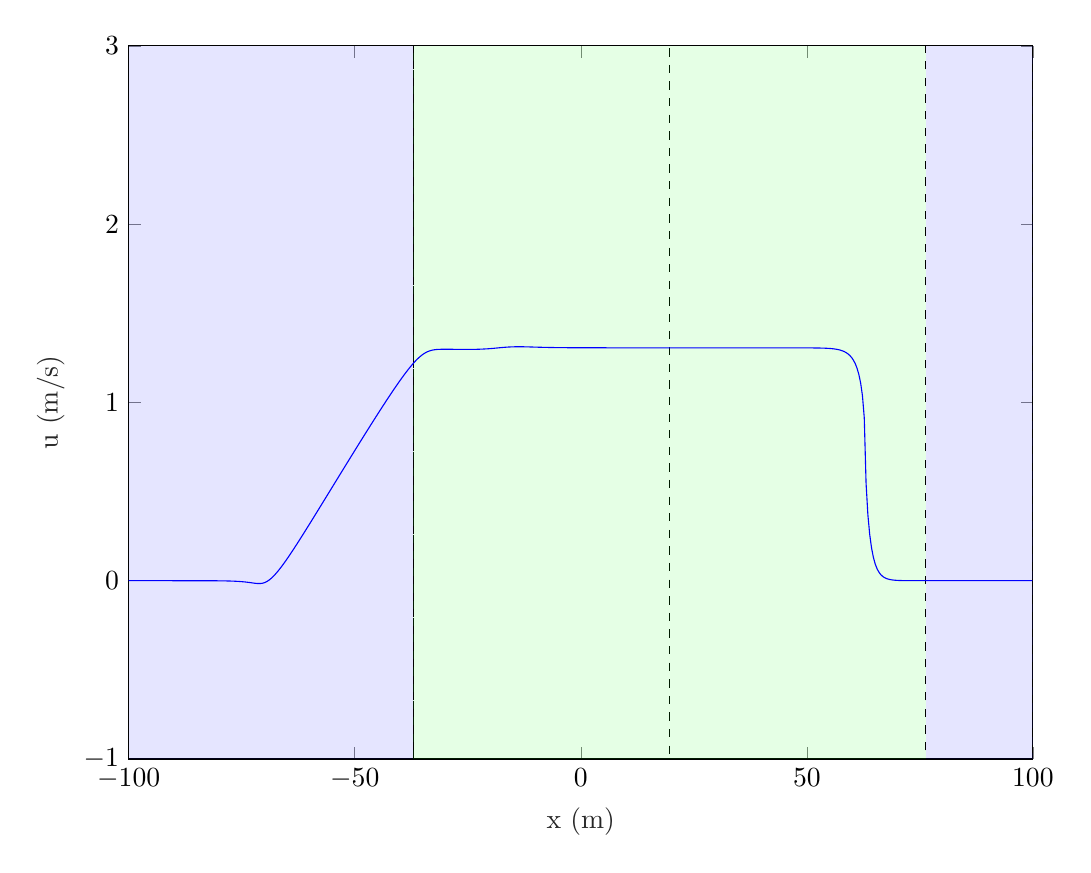
\begin{tikzpicture}

\begin{axis}[%
width=4.521in,
height=3.566in,
at={(0.758in,0.481in)},
scale only axis,
xmin=-100,
xmax=100,
xtick={-100,  -50,    0,   50,  100},
xlabel style={font=\color{white!15!black}},
xlabel={x (m)},
ymin=-1,
ymax=3,
ytick={-1,  0,  1,  2,  3},
ylabel style={font=\color{white!15!black}},
ylabel={u (m/s)},
axis background/.style={fill=white}
]

\addplot[area legend, dashed, draw=black, fill=blue, fill opacity=0.1, forget plot]
table[row sep=crcr] {%
x	y\\
-100	-3\\
-100	3\\
-37.0630892039997	3\\
-37.0630892039997	-3\\
}--cycle;

\addplot[area legend, dashed, draw=black, fill=green, fill opacity=0.1, forget plot]
table[row sep=crcr] {%
x	y\\
-37.0630892039997	-3\\
-37.0630892039997	3\\
19.5890566189392	3\\
19.5890566189392	-3\\
}--cycle;

\addplot[area legend, draw=none, fill=green, fill opacity=0.1, forget plot]
table[row sep=crcr] {%
x	y\\
19.5890566189392	-3\\
19.5890566189392	3\\
76.2412024418781	3\\
76.2412024418781	-3\\
}--cycle;

\addplot[area legend, dashed, draw=black, fill=blue, fill opacity=0.1, forget plot]
table[row sep=crcr] {%
x	y\\
76.2412024418781	-3\\
76.2412024418781	3\\
100	3\\
100	-3\\
}--cycle;
\addplot [color=blue, forget plot]
  table[row sep=crcr]{%
-100.1200120012	0\\
-99.7199719971997	-1.36171330571723e-08\\
-99.3199319931993	-3.86043806432635e-08\\
-98.9198919891989	-8.04975401171462e-08\\
-98.5198519851985	-1.38006123441225e-07\\
-98.1198119811981	-2.10622955427693e-07\\
-97.7197719771977	-2.98555252660792e-07\\
-97.3197319731973	-4.02682967512809e-07\\
-96.9196919691969	-5.24542429009571e-07\\
-96.5196519651965	-6.66333465819747e-07\\
-96.1196119611961	-8.30949463735897e-07\\
-95.7195719571957	-1.022030449519e-06\\
-95.3195319531953	-1.24403957285489e-06\\
-94.9194919491949	-1.50236492257496e-06\\
-94.5194519451945	-1.80344875481825e-06\\
-94.1194119411941	-2.1549471332124e-06\\
-93.7193719371937	-2.56592389178225e-06\\
-93.3193319331933	-3.04708390420881e-06\\
-92.9192919291929	-3.6110516196321e-06\\
-92.5192519251925	-4.27270215084885e-06\\
-92.1192119211921	-5.04955342506242e-06\\
-91.7191719171917	-5.96223002559332e-06\\
-91.3191319131913	-7.03501072124817e-06\\
-90.9190919091909	-8.29647436252028e-06\\
-90.5190519051905	-9.78026134951059e-06\\
-90.1190119011901	-1.15259708949269e-05\\
-89.7189718971897	-1.35802183437606e-05\\
-89.3189318931893	-1.59978801293247e-05\\
-88.9188918891889	-1.88435604834424e-05\\
-88.5188518851885	-2.21933185600337e-05\\
-88.1188118811881	-2.61367024222989e-05\\
-87.7187718771877	-3.07791439252042e-05\\
-87.3187318731873	-3.62447789094053e-05\\
-86.9186918691869	-4.26797682031923e-05\\
-86.5186518651865	-5.02562084076841e-05\\
-86.1186118611861	-5.917673678217e-05\\
-85.7185718571857	-6.96799529770825e-05\\
-85.3185318531853	-8.20468029100796e-05\\
-84.9184918491849	-9.66080938311674e-05\\
-84.5184518451845	-0.000113753340524898\\
-84.1184118411841	-0.000133941176694241\\
-83.7183718371837	-0.000157711604886564\\
-83.3183318331833	-0.000185700405005864\\
-82.9182918291829	-0.000218656075327844\\
-82.5182518251825	-0.000257459732906049\\
-82.1182118211821	-0.000303148480898846\\
-81.7181718171817	-0.000356942806670754\\
-81.3181318131813	-0.000420278656432083\\
-80.9180918091809	-0.000494844920789905\\
-80.5180518051805	-0.000582627104643179\\
-80.1180118011801	-0.000685958027456381\\
-79.7179717971797	-0.000807576387199764\\
-79.3179317931793	-0.000950693903684012\\
-78.9178917891789	-0.00111907161214939\\
-78.5178517851785	-0.00131710540167639\\
-78.1178117811781	-0.00154991959956249\\
-77.7177717771777	-0.001823466705717\\
-77.3177317731773	-0.0021446273134496\\
-76.9176917691769	-0.00252130180129145\\
-76.5176517651765	-0.00296247620978857\\
-76.1176117611761	-0.00347823169500986\\
-75.7175717571757	-0.00407965331404072\\
-75.3175317531753	-0.00477855131919683\\
-74.9174917491749	-0.00558688046485275\\
-74.5174517451745	-0.00651561929822068\\
-74.1174117411741	-0.00757280829700939\\
-73.7173717371737	-0.00876026431641017\\
-73.3173317331733	-0.010068271788174\\
-72.9172917291729	-0.0114675054025247\\
-72.5172517251725	-0.0128976141713181\\
-72.1172117211721	-0.0142530890217991\\
-71.7171717171717	-0.0153695509875106\\
-71.3171317131713	-0.0160160068056466\\
-70.9170917091709	-0.015886321551575\\
-70.5170517051705	-0.014709754355048\\
-70.1170117011701	-0.0122265821941101\\
-69.7169716971697	-0.00827727550621283\\
-69.3169316931693	-0.00281672567331452\\
-68.9168916891689	0.00410068295348886\\
-68.5168516851685	0.0123570167584396\\
-68.1168116811681	0.0218045262843995\\
-67.7167716771677	0.0322898398979848\\
-67.3167316731673	0.0436679298934694\\
-66.9166916691669	0.0558085608486784\\
-66.5166516651665	0.0685982097425687\\
-66.1166116611661	0.0819396226282433\\
-65.7165716571657	0.0957502485750918\\
-65.3165316531653	0.109960265218244\\
-64.9164916491649	0.124510736621502\\
-64.5164516451645	0.139351996481014\\
-64.1164116411641	0.154442097613106\\
-63.7163716371637	0.169745494872318\\
-63.3163316331633	0.185232044578884\\
-62.9162916291629	0.200876118957862\\
-62.5162516251625	0.216655838092714\\
-62.1162116211621	0.232552481389314\\
-61.7161716171617	0.248549987605756\\
-61.3161316131613	0.26463452996825\\
-60.9160916091609	0.280794163934023\\
-60.5160516051605	0.297018526981761\\
-60.1160116011601	0.313298612814737\\
-59.7159715971597	0.3296265569622\\
-59.3159315931593	0.345995472871744\\
-58.9158915891589	0.362399301344585\\
-58.5158515851585	0.37883268984894\\
-58.1158115811581	0.395290888486583\\
-57.7157715771577	0.411769651657719\\
-57.3157315731573	0.42826517932391\\
-56.9156915691569	0.444774051186768\\
-56.5156515651565	0.461293165387447\\
-56.1156115611561	0.477819685396676\\
-55.7155715571557	0.494351004496086\\
-55.3155315531553	0.510884710379248\\
-54.9154915491549	0.527418553648154\\
-54.5154515451545	0.543950421211407\\
-54.1154115411541	0.560478307344351\\
-53.7153715371537	0.577000296944458\\
-53.3153315331533	0.593514553063535\\
-52.9152915291529	0.610019271359759\\
-52.5152515251525	0.626512678349658\\
-52.1152115211521	0.642993020275486\\
-51.7151715171517	0.659458554308463\\
-51.3151315131513	0.675907527854866\\
-50.9150915091509	0.692338150165155\\
-50.5150515051505	0.708748595050329\\
-50.1150115011501	0.72513699391489\\
-49.7149714971497	0.741501402372227\\
-49.3149314931493	0.757839785971804\\
-48.9148914891489	0.774150006251962\\
-48.5148514851485	0.790429804260773\\
-48.1148114811481	0.80667677830861\\
-47.7147714771477	0.822888360464731\\
-47.3147314731473	0.839061804704002\\
-46.9146914691469	0.855194114367692\\
-46.5146514651465	0.871282036869743\\
-46.1146114611461	0.887322038197265\\
-45.7145714571457	0.903310251927707\\
-45.3145314531453	0.919242403505617\\
-44.9144914491449	0.935113791699767\\
-44.5144514451445	0.950919197805741\\
-44.1144114411441	0.966652793123028\\
-43.7143714371437	0.982308052800139\\
-43.3143314331433	0.997877647327927\\
-42.9142914291429	1.01335330320316\\
-42.5142514251425	1.02872566114121\\
-42.1142114211421	1.04398404686152\\
-41.7141714171417	1.05911626175097\\
-41.3141314131413	1.07410835349761\\
-40.9140914091409	1.08894427764597\\
-40.5140514051405	1.1036055290507\\
-40.1140114011401	1.11807073729612\\
-39.7139713971397	1.13231511837756\\
-39.3139313931393	1.14630990250235\\
-38.9138913891389	1.16002167535151\\
-38.5138513851385	1.17341163797752\\
-38.1138113811381	1.18643483823492\\
-37.7137713771377	1.19903933276213\\
-37.3137313731373	1.21116559048393\\
-36.9136913691369	1.2227460928362\\
-36.5136513651365	1.23370544637946\\
-36.1136113611361	1.24396153923479\\
-35.7135713571357	1.25342821322674\\
-35.3135313531353	1.26202001133514\\
-34.9134913491349	1.2696596669195\\
-34.5134513451345	1.27628826160699\\
-34.1134113411341	1.28187672477457\\
-33.7133713371337	1.2864362319037\\
-33.3133313331333	1.29002344826919\\
-32.9132913291329	1.2927372291745\\
-32.5132513251325	1.29470660115615\\
-32.1132113211321	1.29607365447\\
-31.7131713171317	1.29697663076977\\
-31.3131313131313	1.29753776731952\\
-30.9130913091309	1.29785729722206\\
-30.5130513051305	1.29801267712639\\
-30.1130113011301	1.29806134834703\\
-29.7129712971297	1.29804573363\\
-29.3129312931293	1.2979904808609\\
-28.9128912891289	1.29791461408359\\
-28.5128512851285	1.29783040836197\\
-28.1128112811281	1.29774530300629\\
-27.7127712771277	1.29766348331168\\
-27.3127312731273	1.29758714164345\\
-26.9126912691269	1.29751728400211\\
-26.5126512651265	1.29745439792691\\
-26.1126112611261	1.29739896519396\\
-25.7125712571257	1.2973523057046\\
-25.3125312531253	1.29731751136779\\
-24.9124912491249	1.29729815895551\\
-24.5124512451245	1.29730086978518\\
-24.1124112411241	1.29734118451849\\
-23.7123712371237	1.2974334813017\\
-23.3123312331233	1.29759224988726\\
-22.9122912291229	1.29783403250708\\
-22.5122512251225	1.29816957767483\\
-22.1122112211221	1.29858646688119\\
-21.7121712171217	1.29906388993883\\
-21.3121312131213	1.2995831525355\\
-20.9120912091209	1.30012706319379\\
-20.5120512051205	1.3007434507105\\
-20.1120112011201	1.30147484163172\\
-19.7119711971197	1.30230757775694\\
-19.3119311931193	1.30321720854923\\
-18.9118911891189	1.30417449291115\\
-18.5118511851185	1.30515926233934\\
-18.1118111811181	1.30615029785144\\
-17.7117711771177	1.3071212877184\\
-17.3117311731173	1.30804781425408\\
-16.9116911691169	1.30890919113453\\
-16.5116511651165	1.30966802741225\\
-16.1116111611161	1.31031020365086\\
-15.7115711571157	1.31085036798933\\
-15.3115311531153	1.31129703952755\\
-14.9114911491149	1.3116489312749\\
-14.5114511451145	1.31189967332021\\
-14.1114111411141	1.31204875584652\\
-13.7113711371137	1.31210386462291\\
-13.3113311331133	1.31207520208519\\
-12.9112911291129	1.31195857831955\\
-12.5112511251125	1.31178122784604\\
-12.1112111211121	1.31155309211496\\
-11.7111711171117	1.311287967525\\
-11.3111311131113	1.31099870856652\\
-10.9110911091109	1.31069463826987\\
-10.5110511051105	1.31038430709834\\
-10.1110111011101	1.3100745832335\\
-9.71097109710971	1.3097698659421\\
-9.3109310931093	1.30947543729885\\
-8.9108910891089	1.30919384080678\\
-8.51085108510851	1.30892707850205\\
-8.11081108110811	1.30867627576183\\
-7.71077107710771	1.30844238868218\\
-7.31073107310731	1.30822514378913\\
-6.9106910691069	1.30802419066444\\
-6.5106510651065	1.30783920559733\\
-6.11061106110611	1.30766960896346\\
-5.71057105710571	1.30751478489634\\
-5.31053105310531	1.30737383706792\\
-4.91049104910491	1.30724570687505\\
-4.5104510451045	1.30713009206782\\
-4.1104110411041	1.30702571045423\\
-3.71037103710371	1.30693185180739\\
-3.31033103310331	1.30684749529184\\
-2.91029102910291	1.306772013029\\
-2.51025102510251	1.30670448237732\\
-2.1102110211021	1.3066446034709\\
-1.7101710171017	1.30659071698232\\
-1.31013101310131	1.30654269515539\\
-0.91009100910091	1.30650046075505\\
-0.510051005100507	1.30646326773523\\
-0.110011001100105	1.30643031365145\\
0.290029002900297	1.30640094289514\\
0.6900690069007	1.30637447446724\\
1.09010901090109	1.30635045056298\\
1.49014901490149	1.30632899804495\\
1.89018901890189	1.30631025398762\\
2.2902290229023	1.3062928967614\\
2.6902690269027	1.30627722058156\\
3.0903090309031	1.30626294161484\\
3.4903490349035	1.30624970317645\\
3.89038903890389	1.30623729476897\\
4.29042904290429	1.30622547657624\\
4.6904690469047	1.30621445084177\\
5.0905090509051	1.30620392660863\\
5.4905490549055	1.30619349069495\\
5.8905890589059	1.30618344558524\\
6.29062906290629	1.30617351426755\\
6.69066906690669	1.30616339388514\\
7.0907090709071	1.30615412599259\\
7.4907490749075	1.30614463087681\\
7.8907890789079	1.30613488811394\\
8.2908290829083	1.30612550985341\\
8.69086908690869	1.30611635302175\\
9.09090909090909	1.30610718538575\\
9.4909490949095	1.30609787192925\\
9.8909890989099	1.30608850139001\\
10.2910291029103	1.30607916768018\\
10.6910691069107	1.30606990708435\\
11.0911091109111	1.30606092104798\\
11.4911491149115	1.30605228109639\\
11.8911891189119	1.30604412171324\\
12.2912291229123	1.30603622897271\\
12.6912691269127	1.30602837193058\\
13.0913091309131	1.30602009282422\\
13.4913491349135	1.30601195110115\\
13.8913891389139	1.30600445122916\\
14.2914291429143	1.30599744212491\\
14.6914691469147	1.30599020291133\\
15.0915091509151	1.30598302125373\\
15.4915491549155	1.3059765297833\\
15.8915891589159	1.30597006546405\\
16.2916291629163	1.30596378761825\\
16.6916691669167	1.30595789422944\\
17.0917091709171	1.30595208148469\\
17.4917491749175	1.30594658815184\\
17.8917891789179	1.30594128234211\\
18.2918291829183	1.30593616255734\\
18.6918691869187	1.30593136066741\\
19.0919091909191	1.30592669792157\\
19.4919491949195	1.30592226970357\\
19.8919891989199	1.30591811047888\\
20.2920292029203	1.30591407731974\\
20.6920692069207	1.30591035130839\\
21.0921092109211	1.3059066972825\\
21.4921492149215	1.30590337234401\\
21.8921892189219	1.30590001444331\\
22.2922292229223	1.3058970929837\\
22.6922692269227	1.30589408263949\\
23.0923092309231	1.30589140798406\\
23.4923492349235	1.305888805762\\
23.8923892389239	1.30588635775237\\
24.2924292429243	1.30588404987005\\
24.6924692469247	1.30588183103099\\
25.0925092509251	1.30587988581926\\
25.4925492549255	1.30587782058843\\
25.8925892589259	1.30587596025679\\
26.2926292629263	1.30587419745831\\
26.6926692669267	1.3058724761933\\
27.0927092709271	1.30587096707484\\
27.4927492749275	1.30586924903943\\
27.8927892789279	1.30586778062825\\
28.2928292829283	1.30586652515237\\
28.6928692869287	1.30586521283818\\
29.0929092909291	1.30586403218052\\
29.4929492949295	1.30586275130919\\
29.8929892989299	1.30586144048134\\
30.2930293029303	1.30586031903266\\
30.6930693069307	1.30585933295475\\
31.0931093109311	1.30585835237561\\
31.4931493149315	1.30585747937048\\
31.8931893189319	1.30585642883725\\
32.2932293229323	1.30585535931712\\
32.6932693269327	1.30585444450463\\
33.0933093309331	1.30585355677607\\
33.4933493349335	1.30585261352497\\
33.8933893389339	1.30585187330464\\
34.2934293429343	1.30585117803793\\
34.6934693469347	1.30585045195143\\
35.0935093509351	1.30584978438007\\
35.4935493549355	1.30584906851966\\
35.8935893589359	1.30584818222258\\
36.2936293629363	1.30584736896821\\
36.6936693669367	1.30584669088016\\
37.0937093709371	1.30584595403048\\
37.4937493749375	1.30584513280684\\
37.8937893789379	1.30584443476043\\
38.2938293829383	1.30584379390605\\
38.6938693869387	1.305843211875\\
39.0939093909391	1.30584272460557\\
39.4939493949395	1.30584216846799\\
39.8939893989399	1.30584141908997\\
40.2940294029403	1.30584073353521\\
40.6940694069407	1.30584014287055\\
41.0941094109411	1.30583931782403\\
41.4941494149415	1.30583824587012\\
41.8941894189419	1.3058374230843\\
42.2942294229423	1.30583653811662\\
42.6942694269427	1.30583535535079\\
43.0943094309431	1.30583380511927\\
43.4943494349435	1.30583240289405\\
43.8943894389439	1.30583072096629\\
44.2944294429443	1.3058286407365\\
44.6944694469447	1.30582595803827\\
45.0945094509451	1.30582315623874\\
45.4945494549455	1.30581958413422\\
45.8945894589459	1.30581530836768\\
46.2946294629463	1.30580977976536\\
46.6946694669467	1.30580340965401\\
47.0947094709471	1.30579520706555\\
47.4947494749475	1.3057853939333\\
47.8947894789479	1.30577271808929\\
48.2948294829483	1.30575742270188\\
48.6948694869487	1.30573792775973\\
49.0949094909491	1.30571422311038\\
49.4949494949495	1.30568390306491\\
49.8949894989499	1.30564664994452\\
50.2950295029503	1.30559949408586\\
50.6950695069507	1.3055413486637\\
51.0951095109511	1.30546760949675\\
51.4951495149515	1.30537619411716\\
51.8951895189519	1.30526095081423\\
52.2952295229523	1.30511766004889\\
52.6952695269527	1.30493722351941\\
53.0953095309531	1.30471218104175\\
53.4953495349535	1.30442974365222\\
53.8953895389539	1.30407680899638\\
54.2954295429543	1.30363367813601\\
54.6954695469547	1.30307889080148\\
55.0955095509551	1.30238319443149\\
55.4955495549555	1.30151083845052\\
55.8955895589559	1.30041606286762\\
56.2956295629563	1.29904092060112\\
56.6956695669567	1.29731419140536\\
57.0957095709571	1.29514059939439\\
57.4957495749575	1.29240562404719\\
57.8957895789579	1.28895361089113\\
58.2958295829583	1.28459622005019\\
58.6958695869587	1.27907160496474\\
59.0959095909591	1.27205731483877\\
59.4959495949595	1.26309835099228\\
59.8959895989599	1.25161286494192\\
60.2960296029603	1.23675622701038\\
60.6960696069607	1.21737476686809\\
61.0961096109611	1.19170128613847\\
61.4961496149615	1.15702855108909\\
61.8961896189619	1.10862216015684\\
62.2962296229623	1.03713084931818\\
62.6962696269627	0.914464252767662\\
63.0963096309631	0.546360188604767\\
63.4963496349635	0.36969938549438\\
63.8963896389639	0.260198279873676\\
64.2964296429643	0.185397595948234\\
64.6964696469647	0.132819149251402\\
65.0965096509651	0.0954149610904409\\
65.4965496549655	0.0686494940744014\\
65.8965896589659	0.0494367882329877\\
66.2966296629663	0.035620929130273\\
66.6966696669667	0.0256752853514982\\
67.0967096709671	0.0185108985144953\\
67.4967496749675	0.0133477664042973\\
67.8967896789679	0.00962580216270394\\
68.2968296829683	0.00694221547779605\\
68.6968696869687	0.00500705410059942\\
69.0969096909691	0.0036114596350305\\
69.4969496949695	0.00260492260290376\\
69.8969896989699	0.0018789496664515\\
70.2970297029703	0.00135531855274367\\
70.6970697069707	0.000977624019435061\\
71.0971097109711	0.000705188776331408\\
71.4971497149715	0.000508675841517402\\
71.8971897189719	0.000366925936360138\\
72.2972297229723	0.000264677392115959\\
72.6972697269727	0.000190922055606672\\
73.0973097309731	0.000137719661594194\\
73.4973497349735	9.93427591135527e-05\\
73.8973897389739	7.16599986414401e-05\\
74.2974297429743	5.16913166960216e-05\\
74.6974697469747	3.72870953647737e-05\\
75.0975097509751	2.68967388923863e-05\\
75.4975497549755	1.94017445830848e-05\\
75.8975897589759	1.39952930948855e-05\\
76.2976297629763	1.00953935770774e-05\\
76.6976697669767	7.28223249839232e-06\\
77.0977097709771	5.25298115475737e-06\\
77.4977497749775	3.78919674161794e-06\\
77.8977897789779	2.73330737405993e-06\\
78.2978297829783	1.97164986360399e-06\\
78.6978697869787	1.42223419444387e-06\\
79.0979097909791	1.02591751606183e-06\\
79.4979497949795	7.40037590017949e-07\\
79.8979897989799	5.33820332413481e-07\\
80.2980298029803	3.85067123324701e-07\\
80.6980698069807	2.7776515873709e-07\\
81.0981098109811	2.00363734704925e-07\\
81.4981498149815	1.44530816035368e-07\\
81.8981898189819	1.04256179854388e-07\\
82.2982298229823	7.52043831553822e-08\\
82.6982698269827	5.42480868572422e-08\\
83.0983098309831	3.91314400579005e-08\\
83.4983498349835	2.82271488172564e-08\\
83.8983898389839	2.03614193640036e-08\\
84.2984298429843	1.46875441719418e-08\\
84.6984698469847	1.05947302905875e-08\\
85.0985098509851	7.64241197982609e-09\\
85.4985498549855	5.51278329342288e-09\\
85.8985898589859	3.97659828881677e-09\\
86.2986298629863	2.86847910083268e-09\\
86.6986698669867	2.0691465880023e-09\\
87.0987098709871	1.49256856042892e-09\\
87.4987498749875	1.07666344872009e-09\\
87.8987898789879	7.76651805187819e-10\\
88.2988298829883	5.60235241044423e-10\\
88.6988698869887	4.04124658607196e-10\\
89.0989098909891	2.91517110863795e-10\\
89.4989498949895	2.10281695304606e-10\\
89.8989898989899	1.51694563744997e-10\\
90.2990299029903	1.09430048036066e-10\\
90.6990699069907	7.893258391629e-11\\
91.0991099109911	5.69371138366473e-11\\
91.4991499149915	4.10753532842825e-11\\
91.8991899189919	2.96276589584885e-11\\
92.2992299229923	2.13692427966522e-11\\
92.6992699269927	1.54190489397807e-11\\
93.0993099309931	1.11228477333938e-11\\
93.4993499349935	8.03355106204337e-12\\
93.8993899389939	5.79892708741824e-12\\
94.2994299429943	4.19050215363533e-12\\
94.6994699469947	3.01586031402374e-12\\
95.0995099509951	2.17896595531011e-12\\
95.4995499549955	1.57057653828411e-12\\
95.8995899589959	1.13143978435305e-12\\
96.2996299629963	8.0805115739175e-13\\
96.6996699669967	5.81542528359101e-13\\
97.0997099709971	4.17480626204375e-13\\
97.4997499749975	2.9655542244862e-13\\
97.8997899789979	2.12013220487956e-13\\
98.2998299829983	1.42711137911824e-13\\
98.6998699869987	9.29995763623602e-14\\
99.0999099909991	5.67556346952496e-14\\
99.4999499949995	2.36247095143087e-14\\
99.8999899989999	3.35605205513114e-15\\
};
\end{axis}
\end{tikzpicture}%
		\caption{$u$}
	\end{subfigure}
	\caption{Solution of gSGN with $\beta_1 = 3 -\dfrac{2}{3} $ and $\beta_2 = 3$ (Regularised Shallow Water Wave Equations) for smooth dam-break problem at $t=15s$ with inequality regions shown.}
	\label{fig:RegSWWESDB}
\end{figure}

\begin{figure}
	\tikzset{every picture/.style={scale=0.75}}%
	\centering
	\begin{subfigure}{0.49\textwidth}
		\centering
		% This file was created by matlab2tikz.
%
%The latest updates can be retrieved from
%  http://www.mathworks.com/matlabcentral/fileexchange/22022-matlab2tikz-matlab2tikz
%where you can also make suggestions and rate matlab2tikz.
%
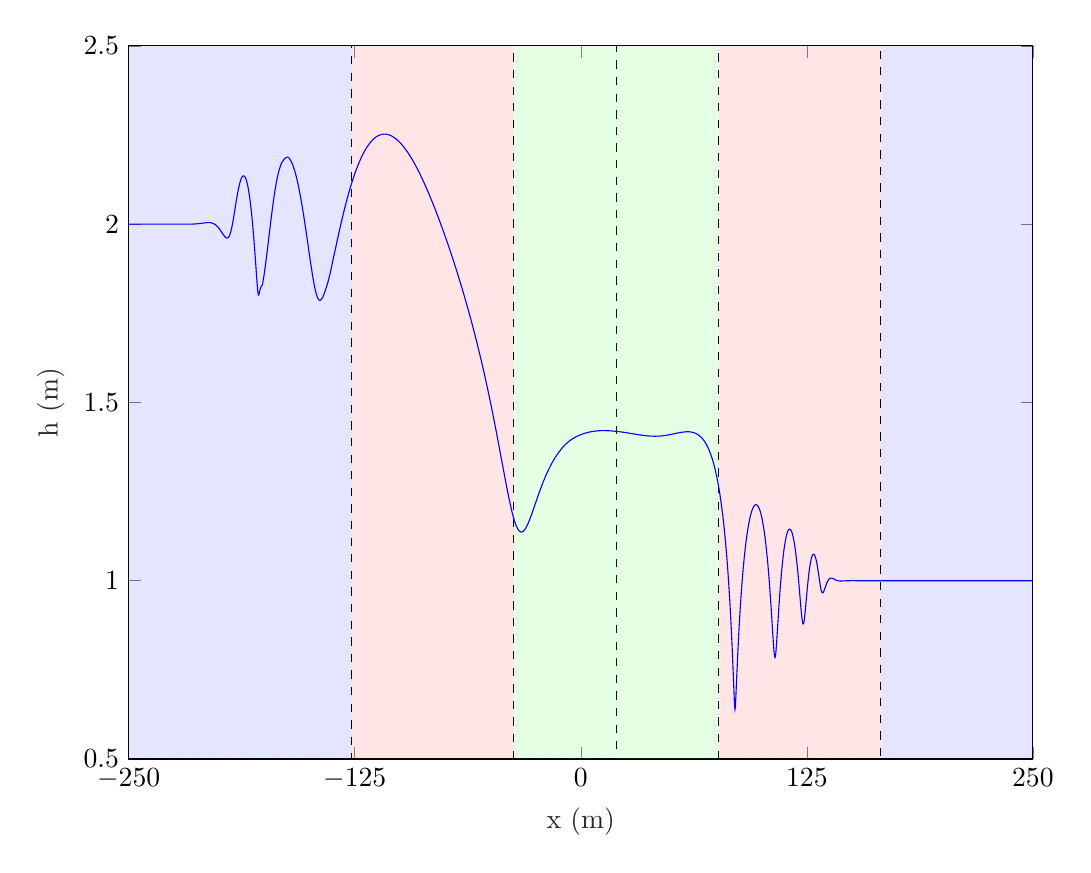
\begin{tikzpicture}

\begin{axis}[%
width=4.521in,
height=3.566in,
at={(0.758in,0.481in)},
scale only axis,
xmin=-250,
xmax=250,
xtick={-250, -125,    0,  125,  250},
xlabel style={font=\color{white!15!black}},
xlabel={x (m)},
ymin=0.5,
ymax=2.5,
ytick={0.5,   1, 1.5,   2, 2.5},
ylabel style={font=\color{white!15!black}},
ylabel={h (m)},
axis background/.style={fill=white}
]

\addplot[area legend, dashed, draw=black, fill=blue, fill opacity=0.1, forget plot]
table[row sep=crcr] {%
x	y\\
-250	0.5\\
-250	2.5\\
-126.679671409596	2.5\\
-126.679671409596	0.5\\
}--cycle;

\addplot[area legend, draw=none, fill=red, fill opacity=0.1, forget plot]
table[row sep=crcr] {%
x	y\\
-126.679671409596	0.5\\
-126.679671409596	2.5\\
-37.0611924008642	2.5\\
-37.0611924008642	0.5\\
}--cycle;

\addplot[area legend, dashed, draw=black, fill=green, fill opacity=0.1, forget plot]
table[row sep=crcr] {%
x	y\\
-37.0611924008642	0.5\\
-37.0611924008642	2.5\\
19.5880540963537	2.5\\
19.5880540963537	0.5\\
}--cycle;

\addplot[area legend, draw=none, fill=green, fill opacity=0.1, forget plot]
table[row sep=crcr] {%
x	y\\
19.5880540963537	0.5\\
19.5880540963537	2.5\\
76.2373005935716	2.5\\
76.2373005935716	0.5\\
}--cycle;

\addplot[area legend, dashed, draw=black, fill=red, fill opacity=0.1, forget plot]
table[row sep=crcr] {%
x	y\\
76.2373005935716	0.5\\
76.2373005935716	2.5\\
165.855779602303	2.5\\
165.855779602303	0.5\\
}--cycle;

\addplot[area legend, draw=none, fill=blue, fill opacity=0.1, forget plot]
table[row sep=crcr] {%
x	y\\
165.855779602303	0.5\\
165.855779602303	2.5\\
250	2.5\\
250	0.5\\
}--cycle;
\addplot [color=blue, forget plot]
  table[row sep=crcr]{%
-250.100003333444	2\\
-249.933331111037	1.99999999561396\\
-249.76665888863	1.99999998856255\\
-249.599986666222	1.99999998219928\\
-249.433314443815	1.99999997653527\\
-249.266642221407	1.999999971582\\
-249.099969999	1.99999996735178\\
-248.933297776593	1.99999996385771\\
-248.766625554185	1.99999996111384\\
-248.599953331778	1.99999995913517\\
-248.43328110937	1.99999995793774\\
-248.266608886963	1.99999995753954\\
-248.099936664555	1.99999995795543\\
-247.933264442148	1.99999995920815\\
-247.766592219741	1.99999996131775\\
-247.599919997333	1.99999996430622\\
-247.433247774926	1.99999996819686\\
-247.266575552518	1.99999997301436\\
-247.099903330111	1.99999997878474\\
-246.933231107704	1.9999999855354\\
-246.766558885296	1.99999999329519\\
-246.599886662889	2.00000000209438\\
-246.433214440481	2.00000001196467\\
-246.266542218074	2.0000000229392\\
-246.099869995667	2.00000003505254\\
-245.933197773259	2.00000004834069\\
-245.766525550852	2.00000006284108\\
-245.599853328444	2.0000000785925\\
-245.433181106037	2.00000009563512\\
-245.266508883629	2.00000011401043\\
-245.099836661222	2.00000013376121\\
-244.933164438815	2.00000015493146\\
-244.766492216407	2.00000017756636\\
-244.599819994	2.00000020171218\\
-244.433147771592	2.00000022741623\\
-244.266475549185	2.00000025472673\\
-244.099803326778	2.00000028369275\\
-243.93313110437	2.00000031436408\\
-243.766458881963	2.00000034679114\\
-243.599786659555	2.00000038102474\\
-243.433114437148	2.00000041711605\\
-243.26644221474	2.00000045511644\\
-243.099769992333	2.00000049507722\\
-242.933097769926	2.00000053704947\\
-242.766425547518	2.00000058108389\\
-242.599753325111	2.00000062723054\\
-242.433081102703	2.00000067553857\\
-242.266408880296	2.00000072605601\\
-242.099736657889	2.00000077882947\\
-241.933064435481	2.00000083390386\\
-241.766392213074	2.00000089132205\\
-241.599719990666	2.00000095112453\\
-241.433047768259	2.00000101334908\\
-241.266375545852	2.00000107803034\\
-241.099703323444	2.00000114519945\\
-240.933031101037	2.00000121488355\\
-240.766358878629	2.00000128710537\\
-240.599686656222	2.00000136188273\\
-240.433014433814	2.00000143922802\\
-240.266342211407	2.00000151914765\\
-240.099669989	2.00000160164146\\
-239.932997766592	2.00000168670212\\
-239.766325544185	2.00000177431459\\
-239.599653321777	2.00000186445532\\
-239.43298109937	2.00000195709158\\
-239.266308876963	2.00000205218074\\
-239.099636654555	2.00000214966949\\
-238.932964432148	2.00000224949301\\
-238.76629220974	2.00000235157412\\
-238.599619987333	2.00000245582251\\
-238.432947764926	2.00000256213364\\
-238.266275542518	2.00000267038789\\
-238.099603320111	2.00000278044955\\
-237.932931097703	2.00000289216579\\
-237.766258875296	2.00000300536556\\
-237.599586652888	2.0000031198584\\
-237.432914430481	2.0000032354334\\
-237.266242208074	2.00000335185798\\
-237.099569985666	2.00000346887662\\
-236.932897763259	2.00000358620963\\
-236.766225540851	2.00000370355176\\
-236.599553318444	2.00000382057088\\
-236.432881096037	2.00000393690655\\
-236.266208873629	2.00000405217016\\
-236.099536651222	2.00000416593797\\
-235.932864428814	2.00000427775767\\
-235.766192206407	2.00000438714163\\
-235.599519983999	2.00000449356466\\
-235.432847761592	2.00000459646702\\
-235.266175539185	2.00000469524833\\
-235.099503316777	2.00000478926856\\
-234.93283109437	2.000004877845\\
-234.766158871962	2.00000496025149\\
-234.599486649555	2.0000050357162\\
-234.432814427148	2.00000510342023\\
-234.26614220474	2.00000516249587\\
-234.099469982333	2.00000521202502\\
-233.932797759925	2.00000525103747\\
-233.766125537518	2.00000527850916\\
-233.599453315111	2.00000529336085\\
-233.432781092703	2.00000529446516\\
-233.266108870296	2.00000528065328\\
-233.099436647888	2.00000525064188\\
-232.932764425481	2.0000052031113\\
-232.766092203073	2.00000513668323\\
-232.599419980666	2.00000504991509\\
-232.432747758259	2.00000494129911\\
-232.266075535851	2.00000480926214\\
-232.099403313444	2.00000465216377\\
-231.932731091036	2.00000446829509\\
-231.766058868629	2.00000425587875\\
-231.599386646222	2.00000401306916\\
-231.432714423814	2.00000373795065\\
-231.266042201407	2.0000034285379\\
-231.099369978999	2.00000308277716\\
-230.932697756592	2.00000269854456\\
-230.766025534184	2.00000227364822\\
-230.599353311777	2.0000018058297\\
-230.43268108937	2.00000129276239\\
-230.266008866962	2.00000073205676\\
-230.099336644555	2.00000012125847\\
-229.932664422147	1.99999945785429\\
-229.76599219974	1.99999873927131\\
-229.599319977333	1.9999979628831\\
-229.432647754925	1.99999712600988\\
-229.265975532518	1.99999622592587\\
-229.09930331011	1.99999525986215\\
-228.932631087703	1.99999422501603\\
-228.765958865296	1.99999311854363\\
-228.599286642888	1.99999193758235\\
-228.432614420481	1.99999067925293\\
-228.265942198073	1.99998934065652\\
-228.099269975666	1.99998791889933\\
-227.932597753258	1.99998641109202\\
-227.765925530851	1.99998481435941\\
-227.599253308444	1.99998312585686\\
-227.432581086036	1.99998134277842\\
-227.265908863629	1.99997946236959\\
-227.099236641221	1.99997748194026\\
-226.932564418814	1.99997539888147\\
-226.765892196407	1.99997321068102\\
-226.599219973999	1.99997091493817\\
-226.432547751592	1.999968509383\\
-226.265875529184	1.9999659918955\\
-226.099203306777	1.99996336052512\\
-225.932531084369	1.99996061351339\\
-225.765858861962	1.99995774931674\\
-225.599186639555	1.99995476662926\\
-225.432514417147	1.99995166440939\\
-225.26584219474	1.99994844190819\\
-225.099169972332	1.99994509869384\\
-224.932497749925	1.99994163468513\\
-224.765825527518	1.99993805018078\\
-224.59915330511	1.99993434589409\\
-224.432481082703	1.99993052298574\\
-224.265808860295	1.99992658309976\\
-224.099136637888	1.99992252840315\\
-223.932464415481	1.99991836162635\\
-223.765792193073	1.99991408609091\\
-223.599119970666	1.9999097057596\\
-223.432447748258	1.99990522529554\\
-223.265775525851	1.99990065008758\\
-223.099103303443	1.99989598630035\\
-222.932431081036	1.99989124092859\\
-222.765758858629	1.9998864218414\\
-222.599086636221	1.99988153783478\\
-222.432414413814	1.99987659868361\\
-222.265742191406	1.99987161519669\\
-222.099069968999	1.99986659927421\\
-221.932397746592	1.99986156395882\\
-221.765725524184	1.99985652348358\\
-221.599053301777	1.99985149333556\\
-221.432381079369	1.99984649033986\\
-221.265708856962	1.9998415326796\\
-221.099036634554	1.99983663996469\\
-220.932364412147	1.99983183330721\\
-220.76569218974	1.99982713536448\\
-220.599019967332	1.99982257039998\\
-220.432347744925	1.9998181643477\\
-220.265675522517	1.99981394486428\\
-220.09900330011	1.99980994137998\\
-219.932331077703	1.99980618516275\\
-219.765658855295	1.99980270936309\\
-219.598986632888	1.99979954906892\\
-219.43231441048	1.9997967413504\\
-219.265642188073	1.9997943253025\\
-219.098969965666	1.99979234208999\\
-218.932297743258	1.99979083498214\\
-218.765625520851	1.99978984938569\\
-218.598953298443	1.99978943316905\\
-218.432281076036	1.99978963402948\\
-218.265608853628	1.99979050484725\\
-218.098936631221	1.99979210039596\\
-217.932264408814	1.99979447709102\\
-217.765592186406	1.99979769356343\\
-217.598919963999	1.99980181046893\\
-217.432247741591	1.99980689077286\\
-217.265575519184	1.9998129994218\\
-217.098903296777	1.99982020353342\\
-216.932231074369	1.99982857210549\\
-216.765558851962	1.99983817615968\\
-216.598886629554	1.99984908850838\\
-216.432214407147	1.99986138365733\\
-216.26554218474	1.9998751377898\\
-216.098869962332	1.9998904284523\\
-215.932197739925	1.99990733456682\\
-215.765525517517	1.99992593614222\\
-215.59885329511	1.99994631408202\\
-215.432181072702	1.99996855003045\\
-215.265508850295	1.9999927260424\\
-215.098836627888	2.00001892437491\\
-214.93216440548	2.00004722717198\\
-214.765492183073	2.00007771608262\\
-214.598819960665	2.00011047197976\\
-214.432147738258	2.00014557462551\\
-214.265475515851	2.00018310217683\\
-214.098803293443	2.00022313073287\\
-213.932131071036	2.00026573393825\\
-213.765458848628	2.00031098244534\\
-213.598786626221	2.00035894335317\\
-213.432114403813	2.00040967966433\\
-213.265442181406	2.00046324968888\\
-213.098769958999	2.00051970637179\\
-212.932097736591	2.00057909662529\\
-212.765425514184	2.00064146062183\\
-212.598753291776	2.00070683104768\\
-212.432081069369	2.00077523231671\\
-212.265408846962	2.00084667973923\\
-212.098736624554	2.00092117866766\\
-211.932064402147	2.0009987236071\\
-211.765392179739	2.00107929730711\\
-211.598719957332	2.0011628697868\\
-211.432047734924	2.00124939732785\\
-211.265375512517	2.001338821668\\
-211.09870329011	2.00143106910548\\
-210.932031067702	2.00152604825874\\
-210.765358845295	2.00162364960593\\
-210.598686622887	2.0017237451293\\
-210.43201440048	2.00182618710687\\
-210.265342178073	2.00193080657833\\
-210.098669955665	2.00203741118632\\
-209.931997733258	2.00214578594924\\
-209.76532551085	2.00225569075618\\
-209.598653288443	2.00236685989254\\
-209.431981066036	2.00247900065274\\
-209.265308843628	2.00259179239675\\
-209.098636621221	2.00270488541176\\
-208.931964398813	2.00281789998065\\
-208.765292176406	2.00293042537605\\
-208.598619953998	2.00304201894019\\
-208.431947731591	2.00315220523087\\
-208.265275509184	2.00326047523057\\
-208.098603286776	2.00336628567439\\
-207.931931064369	2.003469058447\\
-207.765258841961	2.00356818005918\\
-207.598586619554	2.00366300130782\\
-207.431914397147	2.00375283684853\\
-207.265242174739	2.00383696516538\\
-207.098569952332	2.00391462865\\
-206.931897729924	2.00398503359938\\
-206.765225507517	2.00404735052267\\
-206.598553285109	2.00410071481646\\
-206.431881062702	2.00414422724807\\
-206.265208840295	2.00417695482646\\
-206.098536617887	2.00419793237295\\
-205.93186439548	2.00420613632197\\
-205.765192173072	2.00420064823549\\
-205.598519950665	2.00418032450169\\
-205.431847728258	2.00414409678971\\
-205.26517550585	2.00409085699719\\
-205.098503283443	2.0040194810064\\
-204.931831061035	2.00392882401896\\
-204.765158838628	2.00381772591212\\
-204.598486616221	2.00368501572378\\
-204.431814393813	2.00352951375511\\
-204.265142171406	2.00335003570193\\
-204.098469948998	2.00314539764382\\
-203.931797726591	2.0029144201501\\
-203.765125504183	2.00265593349378\\
-203.598453281776	2.00236878282223\\
-203.431781059369	2.00205183400165\\
-203.265108836961	2.00170397962793\\
-203.098436614554	2.00132414539638\\
-202.931764392146	2.00091129698075\\
-202.765092169739	2.00046444735155\\
-202.598419947332	1.99998266445055\\
-202.431747724924	1.99946507924814\\
-202.265075502517	1.99891089420726\\
-202.098403280109	1.99831939247339\\
-201.931731057702	1.99768994769165\\
-201.765058835294	1.99702203387735\\
-201.598386612887	1.99631523586522\\
-201.43171439048	1.99556926066457\\
-201.265042168072	1.99478394951059\\
-201.098369945665	1.99395929058455\\
-200.931697723257	1.99309543157407\\
-200.76502550085	1.99219269399797\\
-200.598353278443	1.99125158771441\\
-200.431681056035	1.99027282695536\\
-200.265008833628	1.98925734757346\\
-200.09833661122	1.98820632431768\\
-199.931664388813	1.98712118721836\\
-199.764992166406	1.98600363934199\\
-199.598319943998	1.98485568042149\\
-199.431647721591	1.98367962854993\\
-199.264975499183	1.98247814156263\\
-199.098303276776	1.9812542393124\\
-198.931631054368	1.98001132929058\\
-198.764958831961	1.97875323299746\\
-198.598286609554	1.97748421144796\\
-198.431614387146	1.97620899288142\\
-198.264942164739	1.97493280150774\\
-198.098269942331	1.97366138528505\\
-197.931597719924	1.97240104527736\\
-197.764925497517	1.97115866396998\\
-197.598253275109	1.9699417333792\\
-197.431581052702	1.96875838017196\\
-197.264908830294	1.96761739025066\\
-197.098236607887	1.96652822875852\\
-196.93156438548	1.96550105461372\\
-196.764892163072	1.96454672958966\\
-196.598219940665	1.96367681859284\\
-196.431547718257	1.96290357457224\\
-196.26487549585	1.96223991966096\\
-196.098203273442	1.96169939803277\\
-195.931531051035	1.96129614448576\\
-195.764858828628	1.96104471965632\\
-195.59818660622	1.96096088893919\\
-195.431514383813	1.9610572890267\\
-195.264842161405	1.96135145500102\\
-195.098169938998	1.96185762372467\\
-194.931497716591	1.96259047422393\\
-194.764825494183	1.96356381890229\\
-194.598153271776	1.96479041011168\\
-194.431481049368	1.96628157036139\\
-194.264808826961	1.96804682739969\\
-194.098136604553	1.97009354857447\\
-193.931464382146	1.97242660142559\\
-193.764792159739	1.97504804651823\\
-193.598119937331	1.97795688823606\\
-193.431447714924	1.9811489086669\\
-193.264775492516	1.98461660641059\\
-193.098103270109	1.98834924802499\\
-192.931431047702	1.9923330166549\\
-192.764758825294	1.99655126317143\\
-192.598086602887	2.00098483809784\\
-192.431414380479	2.0056125032909\\
-192.264742158072	2.01041139108619\\
-192.098069935665	2.01535742777839\\
-191.931397713257	2.02042583118296\\
-191.76472549085	2.02559149957312\\
-191.598053268442	2.03082940575536\\
-191.431381046035	2.03611492002803\\
-191.264708823627	2.04142407760321\\
-191.09803660122	2.04673378691445\\
-190.931364378813	2.05202198648362\\
-190.764692156405	2.05726775240173\\
-190.598019933998	2.06245136110172\\
-190.43134771159	2.0675543204919\\
-190.264675489183	2.07255937222493\\
-190.098003266776	2.07745046740314\\
-189.931331044368	2.08221271931262\\
-189.764658821961	2.08683234436362\\
-189.597986599553	2.09129660922619\\
-189.431314377146	2.09559377256694\\
-189.264642154738	2.09971301457611\\
-189.097969932331	2.10364436466632\\
-188.931297709924	2.10737864045318\\
-188.764625487516	2.11090738075227\\
-188.597953265109	2.11422277811152\\
-188.431281042701	2.1173176383554\\
-188.264608820294	2.12018530807437\\
-188.097936597887	2.122819636351\\
-187.931264375479	2.12521492164251\\
-187.764592153072	2.12736587019026\\
-187.597919930664	2.12926755591478\\
-187.431247708257	2.13091538285878\\
-187.26457548585	2.13230505201336\\
-187.097903263442	2.13343253189683\\
-186.931231041035	2.13429403088267\\
-186.764558818627	2.1348859704788\\
-186.59788659622	2.13520496645146\\
-186.431214373812	2.13524881294519\\
-186.264542151405	2.13501148994788\\
-186.097869928998	2.13449304189416\\
-185.93119770659	2.13368963088613\\
-185.764525484183	2.13259855364688\\
-185.597853261775	2.13121719357146\\
-185.431181039368	2.12954302198585\\
-185.264508816961	2.12757359714917\\
-185.097836594553	2.1253065313541\\
-184.931164372146	2.12273949593635\\
-184.764492149738	2.119870236479\\
-184.597819927331	2.11669654226046\\
-184.431147704923	2.11321624714325\\
-184.264475482516	2.10942725376198\\
-184.097803260109	2.10532751399851\\
-183.931131037701	2.10091502686102\\
-183.764458815294	2.09618787227238\\
-183.597786592886	2.09114420325267\\
-183.431114370479	2.08578224751986\\
-183.264442148072	2.08010034688291\\
-183.097769925664	2.07409696779594\\
-182.931097703257	2.06777070652944\\
-182.764425480849	2.06112033643523\\
-182.597753258442	2.05414484676314\\
-182.431081036035	2.04684346650561\\
-182.264408813627	2.03921573181882\\
-182.09773659122	2.03126155914935\\
-181.931064368812	2.02298130702559\\
-181.764392146405	2.01437588003937\\
-181.597719923997	2.00544687413631\\
-181.43104770159	1.99619673060001\\
-181.264375479183	1.98662892921218\\
-181.097703256775	1.97674826743856\\
-180.931031034368	1.96656118956416\\
-180.76435881196	1.95607622079058\\
-180.597686589553	1.94530456274567\\
-180.431014367146	1.9342608609918\\
-180.264342144738	1.92296424725303\\
-180.097669922331	1.91143982631052\\
-179.930997699923	1.89972076769809\\
-179.764325477516	1.88785132008808\\
-179.597653255108	1.87589135853823\\
-179.430981032701	1.86392337154522\\
-179.264308810294	1.85206347266108\\
-179.097636587886	1.84047928371218\\
-178.930964365479	1.82941934358305\\
-178.764292143071	1.81926035803147\\
-178.597619920664	1.81057359079213\\
-178.430947698257	1.80416878957038\\
-178.264275475849	1.80091973677783\\
-178.097603253442	1.80110149769298\\
-177.930931031034	1.80383882134282\\
-177.764258808627	1.80755281086286\\
-177.59758658622	1.81141110812821\\
-177.430914363812	1.8150064478268\\
-177.264242141405	1.81816060074078\\
-177.097569918997	1.82080975407513\\
-176.93089769659	1.82295071159313\\
-176.764225474182	1.82461869272886\\
-176.597553251775	1.82588754159184\\
-176.430881029368	1.82688855467966\\
-176.26420880696	1.82787002688404\\
-176.097536584553	1.82936785206679\\
-175.930864362145	1.83255016792124\\
-175.764192139738	1.83850955311235\\
-175.597519917331	1.84439843665115\\
-175.430847694923	1.84832563994246\\
-175.264175472516	1.85362091658182\\
-175.097503250108	1.85944712312135\\
-174.930831027701	1.86508788549189\\
-174.764158805294	1.87096854018034\\
-174.597486582886	1.87715024246599\\
-174.430814360479	1.88340130233339\\
-174.264142138071	1.88981217521218\\
-174.097469915664	1.89637286364012\\
-173.930797693256	1.9030275867609\\
-173.764125470849	1.90978775885492\\
-173.597453248442	1.91663461227041\\
-173.430781026034	1.92354839352829\\
-173.264108803627	1.9305231369487\\
-173.097436581219	1.9375445486909\\
-172.930764358812	1.94459982942371\\
-172.764092136405	1.95167905831842\\
-172.597419913997	1.95877069491293\\
-172.43074769159	1.96586412752264\\
-172.264075469182	1.97294924807276\\
-172.097403246775	1.98001612083275\\
-171.930731024367	1.98705512046391\\
-171.76405880196	1.99405683447461\\
-171.597386579553	2.00101223473941\\
-171.430714357145	2.00791253395456\\
-171.264042134738	2.01474930401503\\
-171.09736991233	2.02151429367451\\
-170.930697689923	2.02819958758347\\
-170.764025467516	2.03479750371742\\
-170.597353245108	2.04130067353148\\
-170.430681022701	2.04770199259547\\
-170.264008800293	2.05399465709691\\
-170.097336577886	2.06017219623567\\
-169.930664355479	2.06622845414872\\
-169.763992133071	2.0721575589196\\
-169.597319910664	2.07795399329474\\
-169.430647688256	2.08361255885549\\
-169.263975465849	2.08912837301832\\
-169.097303243441	2.09449690419397\\
-168.930631021034	2.09971396292397\\
-168.763958798627	2.10477570384164\\
-168.597286576219	2.1096786547958\\
-168.430614353812	2.11441968446114\\
-168.263942131404	2.11899601983433\\
-168.097269908997	2.12340528063451\\
-167.93059768659	2.1276454526985\\
-167.763925464182	2.13171494772745\\
-167.597253241775	2.13561256577887\\
-167.430581019367	2.13933755810996\\
-167.26390879696	2.14288963421041\\
-167.097236574552	2.14626893668599\\
-166.930564352145	2.14947611531743\\
-166.763892129738	2.15251234045883\\
-166.59721990733	2.15537938095513\\
-166.430547684923	2.15807957994779\\
-166.263875462515	2.16061593409731\\
-166.097203240108	2.16299208965631\\
-165.930531017701	2.16521241391231\\
-165.763858795293	2.16728198418132\\
-165.597186572886	2.16920671399358\\
-165.430514350478	2.17099333829425\\
-165.263842128071	2.17264937663169\\
-165.097169905664	2.17418315910476\\
-164.930497683256	2.17560377093094\\
-164.763825460849	2.17692086578416\\
-164.597153238441	2.1781445032231\\
-164.430481016034	2.179284854101\\
-164.263808793626	2.18035178538388\\
-164.097136571219	2.1813542319845\\
-163.930464348812	2.18229948245007\\
-163.763792126404	2.18319223982161\\
-163.597119903997	2.18403358943861\\
-163.430447681589	2.18482084025103\\
-163.263775459182	2.18554705898504\\
-163.097103236775	2.18620085214045\\
-162.930431014367	2.18676772750335\\
-162.76375879196	2.18723118471452\\
-162.597086569552	2.18757387382869\\
-162.430414347145	2.18777936313612\\
-162.263742124737	2.18783359909252\\
-162.09706990233	2.18772460658073\\
-161.930397679923	2.18744543220794\\
-161.763725457515	2.18699186679743\\
-161.597053235108	2.18636335613974\\
-161.4303810127	2.18556391974496\\
-161.263708790293	2.18460223167336\\
-161.097036567886	2.18349210213778\\
-160.930364345478	2.18225253405684\\
-160.763692123071	2.18090716670701\\
-160.597019900663	2.1794825674354\\
-160.430347678256	2.17800426030252\\
-160.263675455848	2.17648927993672\\
-160.097003233441	2.1749362421539\\
-159.930331011034	2.17332324918033\\
-159.763658788626	2.17161023415519\\
-159.596986566219	2.16975220138403\\
-159.430314343811	2.16772468791186\\
-159.263642121404	2.16553651198005\\
-159.096969898997	2.16321816108287\\
-158.930297676589	2.16080441633586\\
-158.763625454182	2.15831560610525\\
-158.596953231774	2.15574930155217\\
-158.430281009367	2.15309382415137\\
-158.26360878696	2.15034120997279\\
-158.096936564552	2.14748850792988\\
-157.930264342145	2.14453308089631\\
-157.763592119737	2.14147217506566\\
-157.59691989733	2.13830577462878\\
-157.430247674922	2.135037442378\\
-157.263575452515	2.13167145780319\\
-157.096903230108	2.12821014581564\\
-156.9302310077	2.12465423515505\\
-156.763558785293	2.1210043013035\\
-156.596886562885	2.1172608404415\\
-156.430214340478	2.11342430728265\\
-156.263542118071	2.10949524428388\\
-156.096869895663	2.10547437220648\\
-155.930197673256	2.10136256796006\\
-155.763525450848	2.09716088083545\\
-155.596853228441	2.0928706433002\\
-155.430181006034	2.08849328803849\\
-155.263508783626	2.0840304073362\\
-155.096836561219	2.07948364089657\\
-154.930164338811	2.07485475148734\\
-154.763492116404	2.07014552946334\\
-154.596819893996	2.06535783885726\\
-154.430147671589	2.06049355248044\\
-154.263475449182	2.05555456848462\\
-154.096803226774	2.05054286357644\\
-153.930131004367	2.04546040832225\\
-153.763458781959	2.04030926275859\\
-153.596786559552	2.03509149644842\\
-153.430114337145	2.02980933075446\\
-153.263442114737	2.02446498434677\\
-153.09676989233	2.01906085629369\\
-152.930097669922	2.01359943003616\\
-152.763425447515	2.00808334686801\\
-152.596753225107	2.00251541301167\\
-152.4300810027	1.99689857000429\\
-152.263408780293	1.99123597911544\\
-152.096736557885	1.9855309741553\\
-151.930064335478	1.97978713558519\\
-151.76339211307	1.9740081984911\\
-151.596719890663	1.96819820478445\\
-151.430047668256	1.96236137044554\\
-151.263375445848	1.95650220670359\\
-151.096703223441	1.95062544140829\\
-150.930031001033	1.94473610825025\\
-150.763358778626	1.93883945246745\\
-150.596686556219	1.93294106261181\\
-150.430014333811	1.9270467513596\\
-150.263342111404	1.92116265822134\\
-150.096669888996	1.91529517387141\\
-149.929997666589	1.90945103422575\\
-149.763325444181	1.90363727154991\\
-149.596653221774	1.89786125669017\\
-149.429980999367	1.89213063798281\\
-149.263308776959	1.88645338792138\\
-149.096636554552	1.88083781631879\\
-148.929964332144	1.87529255738463\\
-148.763292109737	1.86982654567448\\
-148.59661988733	1.86444899560716\\
-148.429947664922	1.85916943194251\\
-148.263275442515	1.85399762140911\\
-148.096603220107	1.84894356183797\\
-147.9299309977	1.84401744380628\\
-147.763258775293	1.83922963609182\\
-147.596586552885	1.8345905676641\\
-147.429914330478	1.83011071504526\\
-147.26324210807	1.82580053300204\\
-147.096569885663	1.82167038823508\\
-146.929897663255	1.81773041639083\\
-146.763225440848	1.81399050536893\\
-146.596553218441	1.81046011891422\\
-146.429880996033	1.80714819740093\\
-146.263208773626	1.80406303710856\\
-146.096536551218	1.80121224108956\\
-145.929864328811	1.79860253691873\\
-145.763192106404	1.79623965989641\\
-145.596519883996	1.79412822429868\\
-145.429847661589	1.79227165925022\\
-145.263175439181	1.79067211525293\\
-145.096503216774	1.78933037572547\\
-144.929830994366	1.78824580331955\\
-144.763158771959	1.78741632654379\\
-144.596486549552	1.7868384386756\\
-144.429814327144	1.78650722374413\\
-144.263142104737	1.78641653687465\\
-144.096469882329	1.78655892218905\\
-143.929797659922	1.78692572268329\\
-143.763125437515	1.78750702384584\\
-143.596453215107	1.78829223698177\\
-143.4297809927	1.78927009865506\\
-143.263108770292	1.79042884874834\\
-143.096436547885	1.79175637001787\\
-142.929764325477	1.79324044555101\\
-142.76309210307	1.79486889763575\\
-142.596419880663	1.79662977917634\\
-142.429747658255	1.79851153121792\\
-142.263075435848	1.80050316841586\\
-142.09640321344	1.80259437619781\\
-141.929730991033	1.80477569004345\\
-141.763058768626	1.80703855811261\\
-141.596386546218	1.80937548438149\\
-141.429714323811	1.81178006174937\\
-141.263042101403	1.81424708698035\\
-141.096369878996	1.81677254755095\\
-140.929697656589	1.81935371752972\\
-140.763025434181	1.82198911620877\\
-140.596353211774	1.82467854513048\\
-140.429680989366	1.82742303135104\\
-140.263008766959	1.83022480599163\\
-140.096336544551	1.83308717172507\\
-139.929664322144	1.83601443619979\\
-139.762992099737	1.83901167733592\\
-139.596319877329	1.84208457388651\\
-139.429647654922	1.8452390872928\\
-139.262975432514	1.84848114955973\\
-139.096303210107	1.851816167341\\
-138.9296309877	1.85524859494336\\
-138.762958765292	1.8587813493438\\
-138.596286542885	1.86241523459228\\
-138.429614320477	1.86614834132587\\
-138.26294209807	1.86997556826707\\
-138.096269875663	1.87388822292371\\
-137.929597653255	1.8778739234459\\
-137.762925430848	1.88191671199197\\
-137.59625320844	1.88599759570895\\
-137.429580986033	1.8900953754672\\
-137.262908763625	1.89418791620308\\
-137.096236541218	1.89825367119105\\
-136.929564318811	1.90227344116878\\
-136.762892096403	1.90623217820447\\
-136.596219873996	1.91012087377563\\
-136.429547651588	1.91393873404875\\
-136.262875429181	1.91769452456696\\
-136.096203206774	1.92140823260478\\
-135.929530984366	1.92511144109369\\
-135.762858761959	1.92884500404057\\
-135.596186539551	1.93265155525167\\
-135.429514317144	1.93656139083599\\
-135.262842094736	1.94057528747813\\
-135.096169872329	1.94465761103327\\
-134.929497649922	1.94874358039223\\
-134.762825427514	1.95277684124204\\
-134.596153205107	1.95673715948738\\
-134.429480982699	1.96062797069098\\
-134.262808760292	1.9644568075362\\
-134.096136537885	1.96823736374747\\
-133.929464315477	1.97198733423058\\
-133.76279209307	1.9757242999751\\
-133.596119870662	1.9794637118996\\
-133.429447648255	1.98321362300054\\
-133.262775425848	1.98697283307024\\
-133.09610320344	1.99073270489275\\
-132.929430981033	1.99447929368489\\
-132.762758758625	1.99819828441927\\
-132.596086536218	2.00188096463087\\
-132.42941431381	2.0055259781128\\
-132.262742091403	2.00913672141134\\
-132.096069868996	2.01271853070027\\
-131.929397646588	2.0162779493908\\
-131.762725424181	2.01981938320521\\
-131.596053201773	2.02334409059042\\
-131.429380979366	2.02685016640622\\
-131.262708756959	2.03033380210152\\
-131.096036534551	2.0337911968073\\
-130.929364312144	2.03721974563601\\
-130.762692089736	2.04061832881336\\
-130.596019867329	2.04398723731803\\
-130.429347644921	2.04732775871315\\
-130.262675422514	2.050641414776\\
-130.096003200107	2.05392921889888\\
-129.929330977699	2.05719132642584\\
-129.762658755292	2.06042707058138\\
-129.595986532884	2.06363535932997\\
-129.429314310477	2.06681523483016\\
-129.26264208807	2.0699663041787\\
-129.095969865662	2.07308878567109\\
-128.929297643255	2.07618327341421\\
-128.762625420847	2.0792503403304\\
-128.59595319844	2.08229029920051\\
-128.429280976033	2.08530313746735\\
-128.262608753625	2.0882886189038\\
-128.095936531218	2.09124634601331\\
-127.92926430881	2.09417587894256\\
-127.762592086403	2.09707686001566\\
-127.595919863995	2.09994904472421\\
-127.429247641588	2.10279232141671\\
-127.262575419181	2.10560660021919\\
-127.095903196773	2.10839179576889\\
-126.929230974366	2.11114784731198\\
-126.762558751958	2.1138747024705\\
-126.595886529551	2.11657238800885\\
-126.429214307144	2.11924102509737\\
-126.262542084736	2.12188073879322\\
-126.095869862329	2.12449165532428\\
-125.929197639921	2.12707389279571\\
-125.762525417514	2.12962751847352\\
-125.595853195106	2.13215257473738\\
-125.429180972699	2.13464912161698\\
-125.262508750292	2.13711722875701\\
-125.095836527884	2.13955693478178\\
-124.929164305477	2.14196823922995\\
-124.762492083069	2.14435111361225\\
-124.595819860662	2.14670549664098\\
-124.429147638255	2.14903130543771\\
-124.262475415847	2.15132848849737\\
-124.09580319344	2.15359706409191\\
-123.929130971032	2.15583715612263\\
-123.762458748625	2.15804896457764\\
-123.595786526218	2.16023270391082\\
-123.42911430381	2.16238852200973\\
-123.262442081403	2.16451647522782\\
-123.095769858995	2.16661652608549\\
-122.929097636588	2.16868858660743\\
-122.76242541418	2.17073259355875\\
-122.595753191773	2.17274856648406\\
-122.429080969366	2.1747366349499\\
-122.262408746958	2.17669699462021\\
-122.095736524551	2.17862985095086\\
-121.929064302143	2.1805353727385\\
-121.762392079736	2.18241365770746\\
-121.595719857329	2.18426473131763\\
-121.429047634921	2.18608858811327\\
-121.262375412514	2.18788524701276\\
-121.095703190106	2.18965478027384\\
-120.929030967699	2.19139730854053\\
-120.762358745291	2.1931129700966\\
-120.595686522884	2.19480188762782\\
-120.429014300477	2.19646415261534\\
-120.262342078069	2.19809983770199\\
-120.095669855662	2.19970900854393\\
-119.928997633254	2.20129173997639\\
-119.762325410847	2.20284813518976\\
-119.59565318844	2.20437831937368\\
-119.428980966032	2.20588241123692\\
-119.262308743625	2.20736051329609\\
-119.095636521217	2.20881271341023\\
-118.92896429881	2.21023908374119\\
-118.762292076403	2.21163969439575\\
-118.595619853995	2.21301463851914\\
-118.428947631588	2.21436403044768\\
-118.26227540918	2.21568798797574\\
-118.095603186773	2.21698661423989\\
-117.928930964365	2.21825999710627\\
-117.762258741958	2.21950822668593\\
-117.595586519551	2.22073138949267\\
-117.428914297143	2.22192958801161\\
-117.262242074736	2.22310294422968\\
-117.095569852328	2.22425156996363\\
-116.928897629921	2.22537557426686\\
-116.762225407514	2.22647504936461\\
-116.595553185106	2.22755008024013\\
-116.428880962699	2.22860076637768\\
-116.262208740291	2.22962720685436\\
-116.095536517884	2.23062949938694\\
-115.928864295477	2.2316077441531\\
-115.762192073069	2.23256205609045\\
-115.595519850662	2.23349253664308\\
-115.428847628254	2.23439929084655\\
-115.262175405847	2.23528241323502\\
-115.095503183439	2.23614197462934\\
-114.928830961032	2.23697804712634\\
-114.762158738625	2.23779072187399\\
-114.595486516217	2.23858009494341\\
-114.42881429381	2.2393462620442\\
-114.262142071402	2.24008931176309\\
-114.095469848995	2.24080934643912\\
-113.928797626588	2.24150649777626\\
-113.76212540418	2.242180881544\\
-113.595453181773	2.24283258501203\\
-113.428780959365	2.24346170329463\\
-113.262108736958	2.24406833791517\\
-113.09543651455	2.24465257027294\\
-112.928764292143	2.24521447522254\\
-112.762092069736	2.24575414218627\\
-112.595419847328	2.24627167554865\\
-112.428747624921	2.24676717283724\\
-112.262075402513	2.24724072347359\\
-112.095403180106	2.24769241126001\\
-111.928730957699	2.24812232473202\\
-111.762058735291	2.24853054496558\\
-111.595386512884	2.24891713656137\\
-111.428714290476	2.24928219079932\\
-111.262042068069	2.2496258098324\\
-111.095369845662	2.24994809157501\\
-110.928697623254	2.25024913571819\\
-110.762025400847	2.25052903570428\\
-110.595353178439	2.25078787134881\\
-110.428680956032	2.25102573483939\\
-110.262008733624	2.25124271312863\\
-110.095336511217	2.25143889243514\\
-109.92866428881	2.25161437595908\\
-109.761992066402	2.2517692872914\\
-109.595319843995	2.25190376462418\\
-109.428647621587	2.25201795198226\\
-109.26197539918	2.25211197428335\\
-109.095303176773	2.25218593590696\\
-108.928630954365	2.2522399241298\\
-108.761958731958	2.25227400669482\\
-108.59528650955	2.25228826029373\\
-108.428614287143	2.25228276396708\\
-108.261942064735	2.25225759965968\\
-108.095269842328	2.25221285197428\\
-107.928597619921	2.25214862377588\\
-107.761925397513	2.25206502130879\\
-107.595253175106	2.2519621714881\\
-107.428580952698	2.25184022037758\\
-107.261908730291	2.25169932263408\\
-107.095236507884	2.25153961464136\\
-106.928564285476	2.25136120234239\\
-106.761892063069	2.25116419926751\\
-106.595219840661	2.25094870110842\\
-106.428547618254	2.25071480534752\\
-106.261875395847	2.25046261510541\\
-106.095203173439	2.25019225708028\\
-105.928530951032	2.24990385574946\\
-105.761858728624	2.2495975384777\\
-105.595186506217	2.24927342664422\\
-105.428514283809	2.248931593269\\
-105.261842061402	2.24857211208771\\
-105.095169838995	2.24819511752055\\
-104.928497616587	2.24780065744349\\
-104.76182539418	2.24738866251686\\
-104.595153171772	2.24695914582248\\
-104.428480949365	2.24651221208648\\
-104.261808726958	2.2460479483133\\
-104.09513650455	2.24556644824187\\
-103.928464282143	2.24506787383432\\
-103.761792059735	2.24455239291501\\
-103.595119837328	2.24402014162408\\
-103.42844761492	2.24347121292879\\
-103.261775392513	2.24290570817411\\
-103.095103170106	2.24232363084757\\
-102.928430947698	2.24172511462858\\
-102.761758725291	2.24111009186488\\
-102.595086502883	2.24047861904267\\
-102.428414280476	2.23983097576327\\
-102.261742058069	2.23916696998483\\
-102.095069835661	2.23848619105843\\
-101.928397613254	2.23778883164635\\
-101.761725390846	2.23707518180783\\
-101.595053168439	2.23634535235375\\
-101.428380946032	2.23559940255059\\
-101.261708723624	2.2348374805961\\
-101.095036501217	2.2340599927617\\
-100.928364278809	2.23326700237834\\
-100.761692056402	2.23245822096414\\
-100.595019833994	2.23163351545668\\
-100.428347611587	2.23079304134789\\
-100.26167538918	2.22993709653679\\
-100.095003166772	2.2290660392249\\
-99.9283309443648	2.22818015214533\\
-99.7616587219574	2.22727958705808\\
-99.59498649955	2.2263644289377\\
-99.4283142771426	2.22543477580298\\
-99.2616420547351	2.22449075893589\\
-99.0949698323277	2.22353245254221\\
-98.9282976099203	2.2225598693373\\
-98.7616253875129	2.22157296368407\\
-98.5949531651055	2.22057174071023\\
-98.4282809426981	2.21955633055947\\
-98.2616087202907	2.21852669659293\\
-98.0949364978833	2.21748268951836\\
-97.9282642754758	2.21642442158985\\
-97.7615920530684	2.2153519134496\\
-97.594919830661	2.21426512442109\\
-97.4282476082536	2.213164294981\\
-97.2615753858462	2.21204951678422\\
-97.0949031634388	2.21092085759782\\
-96.9282309410314	2.2097785510021\\
-96.7615587186239	2.20862260438376\\
-96.5948864962165	2.20745311425554\\
-96.4282142738091	2.2062701793788\\
-96.2615420514017	2.20507373800282\\
-96.0948698289943	2.20386392529506\\
-95.9281976065869	2.20264075237436\\
-95.7615253841795	2.2014042247548\\
-95.5948531617721	2.20015446055819\\
-95.4281809393646	2.19889143298487\\
-95.2615087169572	2.19761525035917\\
-95.0948364945498	2.19632598801116\\
-94.9281642721424	2.19502366547797\\
-94.761492049735	2.19370840051564\\
-94.5948198273276	2.19238021545565\\
-94.4281476049202	2.19103917206199\\
-94.2614753825127	2.18968535072963\\
-94.0948031601053	2.18831876214587\\
-93.9281309376979	2.1869394887931\\
-93.7614587152905	2.18554759842752\\
-93.5947864928831	2.18414311490364\\
-93.4281142704757	2.18272612843992\\
-93.2614420480683	2.18129668581657\\
-93.0947698256608	2.17985482534633\\
-92.9280976032534	2.17840062666752\\
-92.761425380846	2.17693412842499\\
-92.5947531584386	2.17545538168337\\
-92.4280809360312	2.17396447185365\\
-92.2614087136238	2.17246149875993\\
-92.0947364912164	2.17094656392172\\
-91.928064268809	2.16941966314327\\
-91.7613920464015	2.16788106076558\\
-91.5947198239941	2.16633068057636\\
-91.4280476015867	2.16476860665257\\
-91.2613753791793	2.16319562094517\\
-91.0947031567719	2.1616110809929\\
-90.9280309343645	2.16001365208401\\
-90.7613587119571	2.15840344672204\\
-90.5946864895496	2.15678163255299\\
-90.4280142671422	2.15514916426593\\
-90.2613420447348	2.15350642474487\\
-90.0946698223274	2.15185350727607\\
-89.92799759992	2.15019041505158\\
-89.7613253775126	2.14851713216466\\
-89.5946531551052	2.14683367566918\\
-89.4279809326977	2.14514011257248\\
-89.2613087102903	2.14343655987593\\
-89.0946364878829	2.1417231842307\\
-88.9279642654755	2.14000015669532\\
-88.7612920430681	2.13826763230425\\
-88.5946198206607	2.13652571132912\\
-88.4279475982533	2.13477444593394\\
-88.2612753758459	2.1330138626095\\
-88.0946031534384	2.13124400379752\\
-87.927930931031	2.12946495277247\\
-87.7612587086236	2.12767683825755\\
-87.5945864862162	2.12587978570729\\
-87.4279142638088	2.12407385113274\\
-87.2612420414014	2.12225896103703\\
-87.094569818994	2.12043488925153\\
-86.9278975965865	2.11860130160357\\
-86.7612253741791	2.11675784129912\\
-86.5945531517717	2.11490421238539\\
-86.4278809293643	2.113040232881\\
-86.2612087069569	2.11116586241129\\
-86.0945364845495	2.10928118582226\\
-85.9278642621421	2.10738637677566\\
-85.7611920397347	2.1054816626031\\
-85.5945198173272	2.10356727879609\\
-85.4278475949198	2.10164342846461\\
-85.2611753725124	2.09971026677609\\
-85.094503150105	2.09776791706319\\
-84.9278309276976	2.09581652106045\\
-84.7611587052902	2.09385630435976\\
-84.5944864828828	2.09188762031972\\
-84.4278142604753	2.08991092054054\\
-84.2611420380679	2.08792666354625\\
-84.0944698156605	2.08593520301561\\
-83.9277975932531	2.0839367094015\\
-83.7611253708457	2.08193116076556\\
-83.5944531484383	2.07991838249616\\
-83.4277809260309	2.07789811685248\\
-83.2611087036234	2.07587008708566\\
-83.094436481216	2.07383402403481\\
-82.9277642588086	2.07178968205042\\
-82.7610920364012	2.06973687044955\\
-82.5944198139938	2.06767550639676\\
-82.4277475915864	2.06560565048577\\
-82.261075369179	2.06352748946605\\
-82.0944031467716	2.06144126461409\\
-81.9277309243641	2.05934717838144\\
-81.7610587019567	2.05724532461658\\
-81.5943864795493	2.05513569214677\\
-81.4277142571419	2.05301822772563\\
-81.2610420347345	2.05089290606608\\
-81.0943698123271	2.04875977797136\\
-80.9276975899197	2.04661896883467\\
-80.7610253675122	2.04447063559045\\
-80.5943531451048	2.04231489592878\\
-80.4276809226974	2.04015180609203\\
-80.26100870029	2.03798135573311\\
-80.0943364778826	2.03580350934872\\
-79.9276642554752	2.03361824252248\\
-79.7609920330678	2.03142552723339\\
-79.5943198106604	2.02922537970312\\
-79.4276475882529	2.02701784665016\\
-79.2609753658455	2.02480296397272\\
-79.0943031434381	2.02258076182369\\
-78.9276309210307	2.02035123812665\\
-78.7609586986233	2.01811437283743\\
-78.5942864762158	2.01587017128364\\
-78.4276142538084	2.01361867226826\\
-78.260942031401	2.01135993180091\\
-78.0942698089936	2.00909399709898\\
-77.9275975865862	2.0068208910383\\
-77.7609253641788	2.00454060188198\\
-77.5942531417714	2.00225315290832\\
-77.4275809193639	1.99995850619803\\
-77.2609086969565	1.99765668395751\\
-77.0942364745491	1.99534772848814\\
-76.9275642521417	1.99303147093226\\
-76.7608920297343	1.99070824470666\\
-76.5942198073269	1.98837781013117\\
-76.4275475849195	1.98603970262294\\
-76.2608753625121	1.98369455364058\\
-76.0942031401046	1.9813432360232\\
-75.9275309176972	1.97898597275612\\
-75.7608586952898	1.97662249326638\\
-75.5941864728824	1.97425237563059\\
-75.427514250475	1.97187525813022\\
-75.2608420280676	1.96949092543653\\
-75.0941698056602	1.96709927683646\\
-74.9274975832527	1.96470028083255\\
-74.7608253608453	1.96229392662548\\
-74.5941531384379	1.95988019867753\\
-74.4274809160305	1.9574591108577\\
-74.2608086936231	1.9550307132737\\
-74.0941364712157	1.95259504163007\\
-73.9274642488083	1.95015208680868\\
-73.7607920264008	1.94770181962154\\
-73.5941198039934	1.94524422415092\\
-73.427447581586	1.94277930093459\\
-73.2607753591786	1.9403070670181\\
-73.0941031367712	1.93782755927684\\
-72.9274309143638	1.93534081826117\\
-72.7607586919564	1.93284687107562\\
-72.594086469549	1.93034572809653\\
-72.4274142471415	1.9278373799437\\
-72.2607420247341	1.92532181320448\\
-72.0940698023267	1.92279901801989\\
-71.9273975799193	1.92026898576682\\
-71.7607253575119	1.91773170829126\\
-71.5940531351045	1.91518717630501\\
-71.4273809126971	1.91263536376619\\
-71.2607086902896	1.91007624861637\\
-71.0940364678822	1.90750978880174\\
-70.9273642454748	1.90493595411243\\
-70.7606920230674	1.90235471118773\\
-70.59401980066	1.89976602940195\\
-70.4273475782526	1.89716988743199\\
-70.2606753558452	1.89456629668728\\
-70.0940031334378	1.89195527227588\\
-69.9273309110303	1.88933673189779\\
-69.7606586886229	1.88671057381414\\
-69.5939864662155	1.88407675975129\\
-69.4273142438081	1.88143529803453\\
-69.2606420214007	1.87878620089989\\
-69.0939697989933	1.87612947103916\\
-68.9272975765859	1.87346501597089\\
-68.7606253541784	1.87079277428979\\
-68.593953131771	1.86811274684832\\
-68.4272809093636	1.86542477054771\\
-68.2606086869562	1.8627287707425\\
-68.0939364645488	1.86002497280436\\
-67.9272642421414	1.85731349395451\\
-67.760592019734	1.85459411427558\\
-67.5939197973265	1.85186652154881\\
-67.4272475749191	1.8491305227014\\
-67.2605753525117	1.84638602870854\\
-67.0939031301043	1.84363297090408\\
-66.9272309076969	1.8408712827102\\
-66.7605586852895	1.8381009082496\\
-66.5938864628821	1.83532180228538\\
-66.4272142404747	1.8325339312127\\
-66.2605420180672	1.82973725401523\\
-66.0938697956598	1.82693172142393\\
-65.9271975732524	1.82411728817799\\
-65.760525350845	1.82129389228498\\
-65.5938531284376	1.81846144992851\\
-65.4271809060302	1.81561988049371\\
-65.2605086836228	1.81276910554186\\
-65.0938364612153	1.80990904485087\\
-64.9271642388079	1.80703960112045\\
-64.7604920164005	1.80416068557603\\
-64.5938197939931	1.80127219794603\\
-64.4271475715857	1.79837406973541\\
-64.2604753491783	1.79546634162289\\
-64.0938031267709	1.79254905808278\\
-63.9271309043635	1.78962222970398\\
-63.760458681956	1.78668582822664\\
-63.5937864595486	1.78373974447045\\
-63.4271142371412	1.78078380919349\\
-63.2604420147338	1.77781785660844\\
-63.0937697923264	1.77484177574262\\
-62.927097569919	1.77185551702231\\
-62.7604253475116	1.76885902840601\\
-62.5937531251041	1.76585219400034\\
-62.4270809026967	1.76283485697467\\
-62.2604086802893	1.75980690656818\\
-62.0937364578819	1.75676833081511\\
-61.9270642354745	1.75371916535396\\
-61.7603920130671	1.75065937890537\\
-61.5937197906597	1.74758881034352\\
-61.4270475682522	1.74450722469696\\
-61.2603753458448	1.74141443847797\\
-61.0937031234374	1.73831037920481\\
-60.92703090103	1.73519503706967\\
-60.7603586786226	1.73206838996259\\
-60.5936864562152	1.72893035508791\\
-60.4270142338078	1.7257807814587\\
-60.2603420114004	1.72261949505628\\
-60.0936697889929	1.71944636880439\\
-59.9269975665855	1.71626134270414\\
-59.7603253441781	1.7130643733629\\
-59.5936531217707	1.70985536534927\\
-59.4269808993633	1.70663416201024\\
-59.2603086769559	1.70340060820865\\
-59.0936364545485	1.70015460453995\\
-58.926964232141	1.6968960797193\\
-58.7602920097336	1.69362492254795\\
-58.5936197873262	1.69034097971724\\
-58.4269475649188	1.68704411255386\\
-58.2602753425114	1.68373422775456\\
-58.093603120104	1.68041124330202\\
-57.9269308976966	1.67707504239909\\
-57.7602586752892	1.67372548656563\\
-57.5935864528817	1.67036246069727\\
-57.4269142304743	1.66698587226416\\
-57.2602420080669	1.66359561102768\\
-57.0935697856595	1.66019154227142\\
-56.9268975632521	1.65677353451284\\
-56.7602253408447	1.65334146693369\\
-56.5935531184373	1.6498952188783\\
-56.4268808960298	1.64643467245848\\
-56.2602086736224	1.64295973116388\\
-56.093536451215	1.63947030742631\\
-55.9268642288076	1.63596629613007\\
-55.7601920064002	1.63244757604439\\
-55.5935197839928	1.6289140119081\\
-55.4268475615854	1.62536545529638\\
-55.2601753391779	1.6218017555145\\
-55.0935031167705	1.61822279154955\\
-54.9268308943631	1.61462849369428\\
-54.7601586719557	1.6110188099213\\
-54.5934864495483	1.60739364893717\\
-54.4268142271409	1.60375286866433\\
-54.2601420047335	1.60009632571767\\
-54.0934697823261	1.59642392472705\\
-53.9267975599186	1.59273560029097\\
-53.7601253375112	1.58903125374007\\
-53.5934531151038	1.58531073675214\\
-53.4267808926964	1.58157391362687\\
-53.260108670289	1.57782071489064\\
-53.0934364478816	1.57405109966125\\
-52.9267642254742	1.57026498736533\\
-52.7600920030667	1.56646227920028\\
-52.5934197806593	1.56264290109982\\
-52.4267475582519	1.55880679665598\\
-52.2600753358445	1.55495387434249\\
-52.0934031134371	1.55108402780268\\
-51.9267308910297	1.54719720575827\\
-51.7600586686223	1.54329338551925\\
-51.5933864462149	1.53937255487197\\
-51.4267142238074	1.53543465606364\\
-51.2600420014	1.53147964187639\\
-51.0933697789926	1.52750748033917\\
-50.9266975565852	1.52351810776835\\
-50.7600253341778	1.5195115364625\\
-50.5933531117704	1.51548773434297\\
-50.426680889363	1.51144668071461\\
-50.2600086669555	1.50738841189689\\
-50.0933364445481	1.50331295607536\\
-49.9266642221407	1.49922036124181\\
-49.7599919997333	1.49511066149776\\
-49.5933197773259	1.49098385923703\\
-49.4266475549185	1.48683999911362\\
-49.2599753325111	1.48267920301776\\
-49.0933031101036	1.47850157940445\\
-48.9266308876962	1.47430718282108\\
-48.7599586652888	1.47009612762002\\
-48.5932864428814	1.46586856930486\\
-48.426614220474	1.46162465084773\\
-48.2599419980666	1.45736448051732\\
-48.0932697756592	1.45308824997757\\
-47.9265975532518	1.44879625859601\\
-47.7599253308443	1.44448871018563\\
-47.5932531084369	1.44016575087624\\
-47.4265808860295	1.43582764765853\\
-47.2599086636221	1.43147475674412\\
-47.0932364412147	1.42710742491287\\
-46.9265642188073	1.42272599743261\\
-46.7598919963999	1.41833082982322\\
-46.5932197739924	1.41392229508943\\
-46.426547551585	1.40950079143446\\
-46.2598753291776	1.40506675044393\\
-46.0932031067702	1.40062066492416\\
-45.9265308843628	1.39616307907535\\
-45.7598586619554	1.39169454611549\\
-45.593186439548	1.38721562650269\\
-45.4265142171406	1.38272693161364\\
-45.2598419947331	1.37822913127462\\
-45.0931697723257	1.37372293085072\\
-44.9264975499183	1.36920906373628\\
-44.7598253275109	1.36468830867613\\
-44.5931531051035	1.36016151492477\\
-44.4264808826961	1.35562957911597\\
-44.2598086602887	1.35109341437034\\
-44.0931364378812	1.34655397416737\\
-43.9264642154738	1.34201228611471\\
-43.7597919930664	1.33746941773617\\
-43.593119770659	1.33292647453797\\
-43.4264475482516	1.32838463166004\\
-43.2597753258442	1.32384513774621\\
-43.0931031034368	1.31930922268844\\
-42.9264308810293	1.31477818631779\\
-42.7597586586219	1.31025338936029\\
-42.5930864362145	1.30573612744389\\
-42.4264142138071	1.30122782569854\\
-42.2597419913997	1.29673021693357\\
-42.0930697689923	1.29224559405056\\
-41.9263975465849	1.28777614955106\\
-41.7597253241775	1.28332284340682\\
-41.59305310177	1.27888686281471\\
-41.4263808793626	1.27447144295636\\
-41.2597086569552	1.27007947277542\\
-41.0930364345478	1.26571204333348\\
-40.9263642121404	1.26137091389828\\
-40.759691989733	1.25705871865688\\
-40.5930197673256	1.25277779530281\\
-40.4263475449181	1.24853050259922\\
-40.2596753225107	1.24431944007288\\
-40.0930031001033	1.24014754351707\\
-39.9263308776959	1.23601736477211\\
-39.7596586552885	1.23193116684582\\
-39.5929864328811	1.2278914623348\\
-39.4263142104737	1.22390130954807\\
-39.2596419880662	1.21996407244605\\
-39.0929697656588	1.21608267432856\\
-38.9262975432514	1.21225971317271\\
-38.759625320844	1.20849796615965\\
-38.5929530984366	1.20480072064842\\
-38.4262808760292	1.20117140501007\\
-38.2596086536218	1.19761289183015\\
-38.0929364312144	1.19412788716828\\
-37.9262642088069	1.19071968647615\\
-37.7595919863995	1.18739167054483\\
-37.5929197639921	1.18414648701696\\
-37.4262475415847	1.18098719329053\\
-37.2595753191773	1.17791721158635\\
-37.0929030967699	1.17493897740215\\
-36.9262308743625	1.17205559486359\\
-36.759558651955	1.1692700050726\\
-36.5928864295476	1.16658466997678\\
-36.4262142071402	1.16400241038165\\
-36.2595419847328	1.16152556799033\\
-36.0928697623254	1.15915677276403\\
-35.926197539918	1.15689820494237\\
-35.7595253175106	1.15475192396542\\
-35.5928530951032	1.15271999167404\\
-35.4261808726957	1.1508041486633\\
-35.2595086502883	1.149005942852\\
-35.0928364278809	1.14732676486526\\
-34.9261642054735	1.14576789114028\\
-34.7594919830661	1.14433034571148\\
-34.5928197606587	1.14301493455622\\
-34.4261475382513	1.14182220591539\\
-34.2594753158438	1.14075250875903\\
-34.0928030934364	1.13980596483658\\
-33.926130871029	1.13898251466185\\
-33.7594586486216	1.13828193167255\\
-33.5927864262142	1.13770360835243\\
-33.4261142038068	1.13724666595554\\
-33.2594419813994	1.13691016767579\\
-33.0927697589919	1.13669305090674\\
-32.9260975365845	1.13659396706028\\
-32.7594253141771	1.13661130193838\\
-32.5927530917697	1.13674331599646\\
-32.4260808693623	1.13698813405322\\
-32.2594086469549	1.13734349366116\\
-32.0927364245475	1.13780709445029\\
-31.9260642021401	1.13837659953701\\
-31.7593919797326	1.13904950315346\\
-31.5927197573252	1.13982304560064\\
-31.4260475349178	1.14069447937726\\
-31.2593753125104	1.14166100549464\\
-31.092703090103	1.14271966041599\\
-30.9260308676956	1.14386741273248\\
-30.7593586452882	1.145101138702\\
-30.5926864228807	1.1464177811406\\
-30.4260142004733	1.14781416331083\\
-30.2593419780659	1.14928705803659\\
-30.0926697556585	1.15083331134525\\
-29.9259975332511	1.1524497147632\\
-29.7593253108437	1.15413311513715\\
-29.5926530884363	1.15588029633703\\
-29.4259808660289	1.1576880592628\\
-29.2593086436214	1.15955322831134\\
-29.092636421214	1.16147273237388\\
-28.9259641988066	1.16344368407458\\
-28.7592919763992	1.16546299812154\\
-28.5926197539918	1.16752764867233\\
-28.4259475315844	1.16963483398467\\
-28.259275309177	1.17178162069364\\
-28.0926030867695	1.17396533249978\\
-27.9259308643621	1.1761832794975\\
-27.7592586419547	1.17843275260146\\
-27.5925864195473	1.18071110621196\\
-27.4259141971399	1.18301591473985\\
-27.2592419747325	1.18534481262366\\
-27.0925697523251	1.18769541506662\\
-26.9258975299176	1.19006549475947\\
-26.7592253075102	1.1924529171829\\
-26.5925530851028	1.19485551442746\\
-26.4258808626954	1.1972713084224\\
-26.259208640288	1.19969834865294\\
-26.0925364178806	1.20213481205558\\
-25.9258641954732	1.20457890215063\\
-25.7591919730658	1.20702881097153\\
-25.5925197506583	1.20948291068103\\
-25.4258475282509	1.21193962793341\\
-25.2591753058435	1.21439748255591\\
-25.0925030834361	1.2168550148235\\
-24.9258308610287	1.21931083529112\\
-24.7591586386213	1.22176370018596\\
-24.5924864162139	1.22421236158285\\
-24.4258141938064	1.22665561887975\\
-24.259141971399	1.22909238068868\\
-24.0924697489916	1.23152157218339\\
-23.9257975265842	1.23394220593253\\
-23.7591253041768	1.23635333537862\\
-23.5924530817694	1.23875402566559\\
-23.425780859362	1.24114345342656\\
-23.2591086369546	1.24352081060479\\
-23.0924364145471	1.24588533678686\\
-22.9257641921397	1.24823636729111\\
-22.7590919697323	1.25057325545682\\
-22.5924197473249	1.25289536881417\\
-22.4257475249175	1.25520201281023\\
-22.2590753025101	1.25749257380992\\
-22.0924030801027	1.25976671526611\\
-21.9257308576952	1.2620240243699\\
-21.7590586352878	1.26426404424846\\
-21.5923864128804	1.26648634889005\\
-21.425714190473	1.26869057407975\\
-21.2590419680656	1.27087640676881\\
-21.0923697456582	1.27304353346458\\
-20.9256975232508	1.27519163283867\\
-20.7590253008433	1.27732047081325\\
-20.5923530784359	1.27942986650423\\
-20.4256808560285	1.28151954543978\\
-20.2590086336211	1.28358926263189\\
-20.0923364112137	1.28563893077863\\
-19.9256641888063	1.28766853209924\\
-19.7589919663989	1.28967789927236\\
-19.5923197439915	1.29166678193356\\
-19.425647521584	1.29363511084603\\
-19.2589752991766	1.29558292106165\\
-19.0923030767692	1.29751017261896\\
-18.9256308543618	1.29941678769373\\
-18.7589586319544	1.30130272072724\\
-18.592286409547	1.3031679696041\\
-18.4256141871396	1.30501254973383\\
-18.2589419647321	1.30683649717089\\
-18.0922697423247	1.30863988853867\\
-17.9255975199173	1.31042277864374\\
-17.7589252975099	1.31218502660347\\
-17.5922530751025	1.31392658560023\\
-17.4255808526951	1.31564771865125\\
-17.2589086302877	1.31734843051956\\
-17.0922364078803	1.31902831193592\\
-16.9255641854728	1.32068770175994\\
-16.7588919630654	1.32232825503545\\
-16.592219740658	1.32395111575089\\
-16.4255475182506	1.32555595137905\\
-16.2588752958432	1.32714221037368\\
-16.0922030734358	1.32871011792323\\
-15.9255308510284	1.33025985704376\\
-15.7588586286209	1.3317903397014\\
-15.5921864062135	1.33329999597585\\
-15.4255141838061	1.33478806753513\\
-15.2588419613987	1.33625430551238\\
-15.0921697389913	1.3376987212854\\
-14.9254975165839	1.33912137507409\\
-14.7588252941765	1.34052312623787\\
-14.592153071769	1.34190698773899\\
-14.4254808493616	1.34327570905742\\
-14.2588086269542	1.34462845999576\\
-14.0921364045468	1.34596197754276\\
-13.9254641821394	1.34727365255414\\
-13.758791959732	1.34856352414865\\
-13.5921197373246	1.34983352551913\\
-13.4254475149172	1.3510859622431\\
-13.2587752925097	1.3523231414454\\
-13.0921030701023	1.35354654807\\
-12.9254308476949	1.35475721587411\\
-12.7587586252875	1.35595665480097\\
-12.5920864028801	1.35714558413537\\
-12.4254141804727	1.35832331820637\\
-12.2587419580653	1.35948930774116\\
-12.0920697356578	1.36064404452682\\
-11.9253975132504	1.36178815309226\\
-11.758725290843	1.36292134410397\\
-11.5920530684356	1.36404248818375\\
-11.4253808460282	1.36515015160365\\
-11.2587086236208	1.3662430543646\\
-11.0920364012134	1.36732037461818\\
-10.9253641788059	1.368381919114\\
-10.7586919563985	1.36942794977494\\
-10.5920197339911	1.3704580976621\\
-10.4253475115837	1.37147135699024\\
-10.2586752891763	1.37246755194331\\
-10.0920030667689	1.37344728086564\\
-9.92533084436144	1.37440991920889\\
-9.75865862195403	1.37535439516812\\
-9.59198639954661	1.37628310243665\\
-9.4253141771392	1.37719943009509\\
-9.25864195473179	1.37810280657749\\
-9.09196973232437	1.37898976927167\\
-8.92529750991696	1.37985823191154\\
-8.75862528750955	1.38070862951138\\
-8.59195306510213	1.38154195417578\\
-8.42528084269472	1.38235943752294\\
-8.2586086202873	1.38316251626097\\
-8.09193639787989	1.38395198241413\\
-7.92526417547248	1.38472848971502\\
-7.75859195306506	1.38549248942438\\
-7.59191973065765	1.38624389012485\\
-7.42524750825024	1.3869829193223\\
-7.25857528584282	1.38771011336387\\
-7.09190306343541	1.38842538734951\\
-6.925230841028	1.38912853939305\\
-6.75855861862058	1.38981972171065\\
-6.59188639621317	1.39049865120755\\
-6.42521417380576	1.39116502518733\\
-6.25854195139834	1.39181915845303\\
-6.09186972899093	1.39246105090941\\
-5.92519750658352	1.39309053868032\\
-5.7585252841761	1.39370827332517\\
-5.59185306176869	1.39431472718\\
-5.42518083936127	1.39490971339489\\
-5.25850861695386	1.39549370683637\\
-5.09183639454645	1.39606745490212\\
-4.92516417213903	1.39663084358092\\
-4.75849194973162	1.39718399655324\\
-4.59181972732421	1.39772758883849\\
-4.42514750491679	1.39826157573778\\
-4.25847528250938	1.39878577414803\\
-4.09180306010197	1.39930083775015\\
-3.92513083769455	1.39980698796725\\
-3.75845861528714	1.40030379956248\\
-3.59178639287973	1.40079163490736\\
-3.42511417047231	1.40127111508742\\
-3.2584419480649	1.40174207918577\\
-3.09176972565749	1.40220444323428\\
-2.92509750325007	1.40265877208632\\
-2.75842528084266	1.40310529856607\\
-2.59175305843524	1.40354410060201\\
-2.42508083602783	1.40397594857952\\
-2.25840861362042	1.40440130016248\\
-2.091736391213	1.40481979097781\\
-1.92506416880559	1.40523105762962\\
-1.75839194639818	1.40563474370426\\
-1.59171972399076	1.40603012352798\\
-1.42504750158335	1.40641648520713\\
-1.25837527917594	1.40679372173064\\
-1.09170305676852	1.40716244631036\\
-0.92503083436111	1.40752336566864\\
-0.758358611953696	1.40787704176776\\
-0.591686389546282	1.40822500837146\\
-0.425014167138869	1.40856877012169\\
-0.258341944731455	1.40890813737849\\
-0.0916697223240419	1.40924350257203\\
0.0750025000833716	1.40957675782557\\
0.241674722490785	1.40990815407935\\
0.408346944898199	1.41023570072191\\
0.575019167305612	1.41055751029755\\
0.741691389713026	1.4108730512895\\
0.908363612120439	1.41118235909313\\
1.07503583452785	1.41148537991195\\
1.24170805693527	1.41178219964476\\
1.40838027934268	1.41207290087477\\
1.57505250175009	1.41235723611455\\
1.74172472415751	1.41263503614777\\
1.90839694656492	1.41290652919622\\
2.07506916897233	1.41317189355179\\
2.24174139137975	1.4134311790867\\
2.40841361378716	1.41368480509519\\
2.57508583619457	1.41393342423329\\
2.74175805860199	1.41417737294557\\
2.9084302810094	1.41441685303105\\
3.07510250341682	1.41465232349495\\
3.24177472582423	1.41488407012927\\
3.40844694823164	1.41511192531634\\
3.57511917063906	1.41533586825961\\
3.74179139304647	1.41555601885549\\
3.90846361545388	1.41577213995888\\
4.0751358378613	1.41598390914988\\
4.24180806026871	1.41619128061681\\
4.40848028267612	1.41639415280686\\
4.57515250508354	1.41659216085622\\
4.74182472749095	1.41678518591322\\
4.90849694989836	1.41697339552294\\
5.07516917230578	1.41715665397105\\
5.24184139471319	1.41733482966898\\
5.4085136171206	1.41750805480282\\
5.57518583952802	1.417676395112\\
5.74185806193543	1.41783961743749\\
5.90853028434285	1.41799800281274\\
6.07520250675026	1.41815160389632\\
6.24187472915764	1.41830035545244\\
6.40854695156509	1.41844441998561\\
6.57521917397247	1.41858386753633\\
6.74189139637991	1.41871890063346\\
6.9085636187873	1.41884939033674\\
7.07523584119474	1.41897544386413\\
7.24190806360212	1.41909720101223\\
7.40858028600957	1.4192144300766\\
7.57525250841695	1.41932727155712\\
7.74192473082439	1.41943582259709\\
7.90859695323178	1.41953985993302\\
8.07526917563922	1.41963954846041\\
8.24194139804661	1.41973494903833\\
8.40861362045405	1.41982589294279\\
8.57528584286143	1.4199126267425\\
8.74195806526888	1.41999515716706\\
8.90863028767626	1.42007342373585\\
9.0753025100837	1.42014758263564\\
9.24197473249109	1.42021752478426\\
9.40864695489853	1.42028353731923\\
9.57531917730591	1.42034571452217\\
9.74199139971336	1.42040374175382\\
9.90866362212074	1.42045782933725\\
10.0753358445282	1.42050818457885\\
10.2420080669356	1.4205549359034\\
10.408680289343	1.42059817744612\\
10.5753525117504	1.42063766748158\\
10.7420247341578	1.42067340479975\\
10.9086969565652	1.42070557792416\\
11.0753691789727	1.42073422268742\\
11.24204140138	1.42075946185079\\
11.4087136237875	1.42078147258416\\
11.5753858461949	1.42080043935704\\
11.7420580686023	1.42081627512416\\
11.9087302910097	1.42082899474443\\
12.0754025134171	1.4208386587994\\
12.2420747358245	1.42084525838603\\
12.408746958232	1.42084890712481\\
12.5754191806394	1.42084961401879\\
12.7420914030468	1.42084744169259\\
12.9087636254542	1.42084241942388\\
13.0754358478616	1.4208345891044\\
13.242108070269	1.42082401003485\\
13.4087802926765	1.42081074400347\\
13.5754525150838	1.42079485943509\\
13.7421247374913	1.42077643364493\\
13.9087969598987	1.42075552457537\\
14.0754691823061	1.42073214749416\\
14.2421414047135	1.42070631381737\\
14.4088136271209	1.42067803574035\\
14.5754858495283	1.4206473032681\\
14.7421580719358	1.42061410682355\\
14.9088302943431	1.42057850081252\\
15.0755025167506	1.4205406469771\\
15.242174739158	1.42050066926469\\
15.4088469615654	1.42045852347109\\
15.5755191839728	1.42041405519106\\
15.7421914063802	1.42036723552082\\
15.9088636287876	1.42031827627261\\
16.0755358511951	1.42026732835012\\
16.2422080736025	1.42021436013931\\
16.4088802960099	1.42015928640742\\
16.5755525184173	1.42010209883667\\
16.7422247408247	1.42004305358637\\
16.9088969632321	1.41998227263382\\
17.0755691856396	1.41991959568786\\
17.2422414080469	1.41985520398149\\
17.4089136304544	1.41978929965742\\
17.5755858528618	1.41972170161881\\
17.7422580752692	1.4196523995934\\
17.9089302976766	1.41958158617038\\
18.075602520084	1.41950926216044\\
18.2422747424914	1.41943547705066\\
18.4089469648989	1.41936027174079\\
18.5756191873062	1.41928348696932\\
18.7422914097137	1.41920516569815\\
18.9089636321211	1.41912527230831\\
19.0756358545285	1.4190437183459\\
19.2423080769359	1.41896060342864\\
19.4089802993433	1.4188758763131\\
19.5756525217507	1.41878961134515\\
19.7423247441582	1.4187019095201\\
19.9089969665656	1.41861276459056\\
20.075669188973	1.41852219933146\\
20.2423414113804	1.41843019588482\\
20.4090136337878	1.41833675076088\\
20.5756858561952	1.41824184650043\\
20.7423580786026	1.41814547410908\\
20.90903030101	1.41804761460803\\
21.0757025234175	1.41794825687484\\
21.2423747458249	1.41784741067387\\
21.4090469682323	1.41774515270927\\
21.5757191906397	1.41764154569922\\
21.7423914130471	1.41753654235783\\
21.9090636354545	1.41743004701568\\
22.075735857862	1.41732205774815\\
22.2424080802693	1.41721262686178\\
22.4090803026768	1.41710175539138\\
22.5757525250842	1.41698942465167\\
22.7424247474916	1.41687560951609\\
22.909096969899	1.41676021439678\\
23.0757691923064	1.41664302935207\\
23.2424414147139	1.41652389553254\\
23.4091136371213	1.41640289468139\\
23.5757858595287	1.4162802963807\\
23.7424580819361	1.41615641010894\\
23.9091303043435	1.41603141645884\\
24.0758025267509	1.41590538273354\\
24.2424747491584	1.41577839134535\\
24.4091469715657	1.41565053289842\\
24.5758191939732	1.41552186018742\\
24.7424914163806	1.4153922931501\\
24.909163638788	1.41526162006028\\
25.0758358611954	1.41512970866566\\
25.2425080836028	1.41499661215436\\
25.4091803060102	1.41486247033566\\
25.5758525284177	1.4147272235127\\
25.7425247508251	1.41459061382937\\
25.9091969732325	1.41445245689909\\
26.0758691956399	1.41431267060595\\
26.2425414180473	1.41417136143349\\
26.4092136404547	1.41402902072893\\
26.5758858628622	1.41388625815919\\
26.7425580852695	1.41374329811412\\
26.909230307677	1.41359994463811\\
27.0759025300844	1.41345601919621\\
27.2425747524918	1.41331157964669\\
27.4092469748992	1.41316685109982\\
27.5759191973066	1.41302212176414\\
27.742591419714	1.41287758517448\\
27.9092636421215	1.41273337258318\\
28.0759358645288	1.41258945955072\\
28.2426080869363	1.41244560994501\\
28.4092803093437	1.41230160413463\\
28.5759525317511	1.41215747261895\\
28.7426247541585	1.41201348539083\\
28.9092969765659	1.41186974512523\\
29.0759691989733	1.41172622754487\\
29.2426414213808	1.41158299580834\\
29.4093136437882	1.41144013078638\\
29.5759858661956	1.41129772427984\\
29.742658088603	1.41115579672044\\
29.9093303110104	1.41101437923965\\
30.0760025334178	1.41087351381321\\
30.2426747558252	1.41073335181534\\
30.4093469782326	1.41059394184033\\
30.5760192006401	1.41045516751282\\
30.7426914230475	1.4103171104314\\
30.9093636454549	1.4101799488671\\
31.0760358678623	1.41004376523138\\
31.2427080902697	1.40990870471424\\
31.4093803126771	1.40977483822659\\
31.5760525350846	1.40964195596897\\
31.7427247574919	1.40950989373052\\
31.9093969798994	1.40937877463833\\
32.0760692023068	1.40924880430984\\
32.2427414247142	1.40912002393926\\
32.4094136471216	1.40899236564159\\
32.576085869529	1.40886578995258\\
32.7427580919364	1.40874035218175\\
32.9094303143439	1.40861616320063\\
33.0761025367513	1.4084933873191\\
33.2427747591587	1.40837202514741\\
33.4094469815661	1.40825204572754\\
33.5761192039735	1.40813358615539\\
33.7427914263809	1.40801672788875\\
33.9094636487883	1.40790152621458\\
34.0761358711957	1.40778805119098\\
34.2428080936032	1.40767641188619\\
34.4094803160106	1.40756675375791\\
34.576152538418	1.40745909081881\\
34.7428247608254	1.40735345310975\\
34.9094969832328	1.40724987362365\\
35.0761692056402	1.4071481779351\\
35.2428414280477	1.4070482889173\\
35.409513650455	1.40695032039757\\
35.5761858728625	1.40685427494282\\
35.7428580952699	1.40676024281104\\
35.9095303176773	1.40666854065031\\
36.0762025400847	1.40657931092108\\
36.2428747624921	1.4064924261499\\
36.4095469848995	1.40640787423911\\
36.576219207307	1.40632579358131\\
36.7428914297143	1.40624623062313\\
36.9095636521218	1.40616919065921\\
37.0762358745292	1.40609480771274\\
37.2429080969366	1.40602332808248\\
37.409580319344	1.40595489154953\\
37.5762525417514	1.40588941046851\\
37.7429247641588	1.40582667805792\\
37.9095969865663	1.40576657545117\\
38.0762692089737	1.40570924456982\\
38.2429414313811	1.40565502533717\\
38.4096136537885	1.40560415179276\\
38.5762858761959	1.40555662113385\\
38.7429580986033	1.40551236998073\\
38.9096303210108	1.40547129865008\\
39.0763025434181	1.40543324423375\\
39.2429747658256	1.40539816206082\\
39.409646988233	1.40536612845216\\
39.5763192106404	1.40533722125071\\
39.7429914330478	1.40531148820811\\
39.9096636554552	1.40528884677951\\
40.0763358778626	1.40526918390106\\
40.2430081002701	1.40525257328688\\
40.4096803226774	1.40523906835247\\
40.5763525450849	1.40522868166429\\
40.7430247674923	1.40522143612118\\
40.9096969898997	1.40521734969248\\
41.0763692123071	1.40521658107807\\
41.2430414347145	1.40521935348014\\
41.4097136571219	1.40522579934647\\
41.5763858795294	1.40523596980741\\
41.7430581019368	1.40524985462757\\
41.9097303243442	1.40526742203608\\
42.0764025467516	1.40528868576082\\
42.243074769159	1.40531361544126\\
42.4097469915664	1.40534215101278\\
42.5764192139738	1.40537432062184\\
42.7430914363812	1.4054101666021\\
42.9097636587887	1.40544966958741\\
43.0764358811961	1.40549286477602\\
43.2431081036035	1.40553976312596\\
43.4097803260109	1.40559029996533\\
43.5764525484183	1.40564450944164\\
43.7431247708257	1.40570242308761\\
43.9097969932332	1.40576402719872\\
44.0764692156405	1.4058293727226\\
44.243141438048	1.40589845253066\\
44.4098136604554	1.40597123066091\\
44.5764858828628	1.40604769980472\\
44.7431581052702	1.40612781311841\\
44.9098303276776	1.40621153041153\\
45.076502550085	1.40629886558614\\
45.2431747724925	1.40638976777461\\
45.4098469948999	1.40648419478484\\
45.5765192173073	1.40658211241944\\
45.7431914397147	1.40668347969412\\
45.9098636621221	1.4067883115567\\
46.0765358845295	1.40689653863697\\
46.2432081069369	1.4070080963016\\
46.4098803293443	1.40712293413892\\
46.5765525517518	1.40724099481185\\
46.7432247741592	1.40736228456966\\
46.9098969965666	1.40748674031804\\
47.076569218974	1.40761431258244\\
47.2432414413814	1.40774497903506\\
47.4099136637888	1.40787874813039\\
47.5765858861963	1.40801554819572\\
47.7432581086036	1.40815527504177\\
47.9099303310111	1.40829787133958\\
48.0766025534185	1.40844330325284\\
48.2432747758259	1.40859155191102\\
48.4099469982333	1.40874257690156\\
48.5766192206407	1.40889628981735\\
48.7432914430481	1.40905254819958\\
48.9099636654556	1.4092112298803\\
49.0766358878629	1.40937226689494\\
49.2433081102704	1.40953557510888\\
49.4099803326778	1.40970102997778\\
49.5766525550852	1.40986850415525\\
49.7433247774926	1.41003789775925\\
49.9099969999	1.41020913272067\\
50.0766692223074	1.41038208536425\\
50.2433414447149	1.41055663396525\\
50.4100136671223	1.41073267215838\\
50.5766858895297	1.4109101083825\\
50.7433581119371	1.41108886814496\\
50.9100303343445	1.41126884063204\\
51.0767025567519	1.41144991043384\\
51.2433747791594	1.41163193492408\\
51.4100470015667	1.4118147491308\\
51.5767192239742	1.41199822586216\\
51.7433914463816	1.41218219598986\\
51.910063668789	1.41236643781444\\
52.0767358911964	1.41255077346588\\
52.2434081136038	1.41273501186266\\
52.4100803360112	1.41291890696218\\
52.5767525584187	1.41310224547406\\
52.743424780826	1.41328480075061\\
52.9100970032335	1.4134662464649\\
53.0767692256409	1.41364627123645\\
53.2434414480483	1.41382468187151\\
53.4101136704557	1.41400138418352\\
53.5767858928631	1.41417638657154\\
53.7434581152705	1.41434972887228\\
53.910130337678	1.41452130243638\\
54.0768025600854	1.41469082165687\\
54.2434747824928	1.4148579661175\\
54.4101470049002	1.41502241070225\\
54.5768192273076	1.41518387730313\\
54.743491449715	1.41534220847681\\
54.9101636721225	1.41549720926125\\
55.0768358945298	1.41564849598928\\
55.2435081169373	1.41579566728815\\
55.4101803393447	1.41593845551966\\
55.5768525617521	1.41607666526053\\
55.7435247841595	1.4162101323459\\
55.9101970065669	1.41633864857153\\
56.0768692289743	1.41646192898006\\
56.2435414513818	1.41657972461719\\
56.4102136737891	1.41669195009318\\
56.5768858961966	1.41679866029793\\
56.743558118604	1.41689998937968\\
56.9102303410114	1.4169960863234\\
57.0769025634188	1.4170870526121\\
57.2435747858262	1.41717290711534\\
57.4102470082336	1.4172535845545\\
57.5769192306411	1.41732898084073\\
57.7435914530485	1.41739887582423\\
57.9102636754559	1.41746284736228\\
58.0769358978633	1.41752045375866\\
58.2436081202707	1.41757126217848\\
58.4102803426781	1.41761475607024\\
58.5769525650855	1.41765038687917\\
58.7436247874929	1.41767759911534\\
58.9102970099004	1.41769584881479\\
59.0769692323078	1.41770456851088\\
59.2436414547152	1.41770324573842\\
59.4103136771226	1.41769140018795\\
59.57698589953	1.41766852027392\\
59.7436581219374	1.41763408607945\\
59.9103303443449	1.41758762328663\\
60.0770025667522	1.41752868948925\\
60.2436747891597	1.41745685765692\\
60.4103470115671	1.41737175470665\\
60.5770192339745	1.4172730543486\\
60.7436914563819	1.41716044598792\\
60.9103636787893	1.41703361607759\\
61.0770359011967	1.41689226470508\\
61.2437081236042	1.41673610813922\\
61.4103803460116	1.41656489207709\\
61.577052568419	1.41637837633489\\
61.7437247908264	1.4161763037303\\
61.9103970132338	1.41595843138869\\
62.0770692356412	1.41572451332033\\
62.2437414580486	1.41547430482775\\
62.410413680456	1.41520752586531\\
62.5770859028635	1.41492389396442\\
62.7437581252709	1.41462319538859\\
62.9104303476783	1.41430515450458\\
63.0771025700857	1.41396944207197\\
63.2437747924931	1.41361562228509\\
63.4104470149005	1.4132433550173\\
63.577119237308	1.41285225323283\\
63.7437914597153	1.41244187730793\\
63.9104636821228	1.4120117759377\\
64.0771359045302	1.41156139157085\\
64.2438081269376	1.41109031557061\\
64.410480349345	1.41059793208106\\
64.5771525717524	1.41008369137185\\
64.7438247941598	1.40954705005757\\
64.9104970165673	1.40898725535131\\
65.0771692389746	1.40840384386041\\
65.2438414613821	1.40779602056554\\
65.4105136837895	1.40716304894402\\
65.5771859061969	1.40650440866995\\
65.7438581286043	1.40581913445\\
65.9105303510117	1.405106598876\\
66.0772025734191	1.40436602294348\\
66.2438747958266	1.40359642812181\\
66.410547018234	1.40279723889907\\
66.5772192406414	1.40196744462595\\
66.7438914630488	1.40110619993931\\
66.9105636854562	1.40021286270424\\
67.0772359078636	1.39928616923981\\
67.2439081302711	1.39832542691679\\
67.4105803526784	1.39733006873635\\
67.5772525750859	1.39629844266951\\
67.7439247974933	1.39522973663674\\
67.9105970199007	1.39412391627387\\
68.0772692423081	1.392978952939\\
68.2439414647155	1.39179323995535\\
68.4106136871229	1.39056750392737\\
68.5772859095304	1.38930062254766\\
68.7439581319377	1.38798942821941\\
68.9106303543452	1.38663329806547\\
69.0773025767526	1.38523421632988\\
69.24397479916	1.38379002943973\\
69.4106470215674	1.38229602435783\\
69.5773192439748	1.38075232888431\\
69.7439914663822	1.37916199103672\\
69.9106636887897	1.37752320220864\\
70.0773359111971	1.37583092295026\\
70.2440081336045	1.37408216046682\\
70.4106803560119	1.37227827848317\\
70.5773525784193	1.37042295550053\\
70.7440248008267	1.36851511835094\\
70.9106970232341	1.36654725410277\\
71.0773692456415	1.36451420064138\\
71.244041468049	1.36241838243455\\
71.4107136904564	1.36026363346379\\
71.5773859128638	1.35804952379207\\
71.7440581352712	1.35577242723519\\
71.9107303576786	1.35342804821383\\
72.077402580086	1.35101272365488\\
72.2440748024935	1.34852384676812\\
72.4107470249008	1.3459606207494\\
72.5774192473083	1.34332416366254\\
72.7440914697157	1.34061553988949\\
72.9107636921231	1.33783398377982\\
73.0774359145305	1.334976805249\\
73.2441081369379	1.33204036566062\\
73.4107803593453	1.32902111187581\\
73.5774525817528	1.32591585677806\\
73.7441248041602	1.32272137027393\\
73.9107970265676	1.31943551463578\\
74.077469248975	1.31605694494192\\
74.2441414713824	1.31258317142086\\
74.4108136937898	1.30901181396697\\
74.5774859161972	1.30534135904772\\
74.7441581386046	1.30156859111343\\
74.9108303610121	1.29769178272246\\
75.0775025834195	1.29371231183277\\
75.2441748058269	1.28962574930458\\
75.4108470282343	1.28542433277065\\
75.5775192506417	1.28110394959652\\
75.7441914730491	1.27666281113476\\
75.9108636954566	1.27210096509365\\
76.0775359178639	1.26742051616232\\
76.2442081402714	1.26261984419226\\
76.4108803626788	1.25768761167278\\
76.5775525850862	1.25260881843171\\
76.7442248074936	1.24738232253516\\
76.910897029901	1.24201771892678\\
77.0775692523084	1.2365063757541\\
77.2442414747159	1.23083245432407\\
77.4109136971232	1.22499872338748\\
77.5775859195307	1.21900304246662\\
77.7442581419381	1.21283503174384\\
77.9109303643455	1.20649169034299\\
78.0776025867529	1.19996775863597\\
78.2442748091603	1.19325698246675\\
78.4109470315677	1.18635373999723\\
78.5776192539752	1.17925182243924\\
78.7442914763826	1.17194476053784\\
78.91096369879	1.16442565110137\\
79.0776359211974	1.15668732770256\\
79.2443081436048	1.14872229563406\\
79.4109803660122	1.14052260043873\\
79.5776525884197	1.13207973494595\\
79.744324810827	1.12338490596284\\
79.9109970332345	1.1144290132899\\
80.0776692556419	1.1052023716512\\
80.2443414780493	1.09569477833929\\
80.4110137004567	1.0858954414502\\
80.5776859228641	1.07579268845265\\
80.7443581452715	1.06537458158691\\
80.911030367679	1.05462846494517\\
81.0777025900863	1.04354085238392\\
81.2443748124938	1.0320977698408\\
81.4110470349012	1.0202841837684\\
81.5777192573086	1.00808426469234\\
81.744391479716	0.995481773286485\\
81.9110637021234	0.982458740195127\\
82.0777359245308	0.968996678712241\\
82.2444081469383	0.955076651675445\\
82.4110803693457	0.940677803309705\\
82.5777525917531	0.925778934238036\\
82.7444248141605	0.910358348427747\\
82.9110970365679	0.894394209856553\\
83.0777692589753	0.877864149874973\\
83.2444414813828	0.860746964488573\\
83.4111137037901	0.843021653102144\\
83.5777859261976	0.824672782479655\\
83.744458148605	0.80568967293739\\
83.9111303710124	0.786072340649767\\
84.0778025934198	0.765841739552607\\
84.2444748158272	0.745049933573631\\
84.4111470382346	0.723817211051771\\
84.5778192606421	0.702390165870239\\
84.7444914830494	0.681270991576858\\
84.9111637054569	0.661568882543677\\
85.0778359278643	0.645863413590759\\
85.2445081502717	0.639099270229566\\
85.4111803726791	0.644257448287589\\
85.5778525950865	0.65777056291752\\
85.7445248174939	0.675190288851726\\
85.9111970399014	0.694218149477576\\
86.0778692623088	0.713767151070195\\
86.2445414847162	0.733301910425097\\
86.4112137071236	0.752545252604526\\
86.577885929531	0.771349804658602\\
86.7445581519384	0.789637878113683\\
86.9112303743458	0.807371112242302\\
87.0779025967532	0.824534143255378\\
87.2445748191607	0.841125389941062\\
87.4112470415681	0.857151638322113\\
87.5779192639755	0.872624682740203\\
87.7445914863829	0.887559253154875\\
87.9112637087903	0.901971725601779\\
88.0779359311977	0.915879239965488\\
88.2446081536052	0.929299132631134\\
88.4112803760125	0.942248611482235\\
88.57795259842	0.954744483606199\\
88.7446248208274	0.966802998695791\\
88.9112970432348	0.978439804135441\\
89.0779692656422	0.9896698615536\\
89.2446414880496	1.00050744909586\\
89.411313710457	1.01096613780468\\
89.5779859328645	1.0210587766961\\
89.7446581552718	1.0307975945811\\
89.9113303776793	1.04019419515882\\
90.0780026000867	1.04925953025328\\
90.2446748224941	1.05800399610676\\
90.4113470449015	1.06643738320277\\
90.5780192673089	1.07456893930434\\
90.7446914897163	1.08240743938706\\
90.9113637121238	1.08996113861075\\
91.0780359345312	1.09723782184856\\
91.2447081569386	1.10424479225439\\
91.411380379346	1.11098895895536\\
91.5780526017534	1.11747681632842\\
91.7447248241609	1.12371446338722\\
91.9113970465683	1.12970759515173\\
92.0780692689757	1.13546161031299\\
92.2447414913831	1.14098155790374\\
92.4114137137905	1.14627216259825\\
92.5780859361979	1.15133784044574\\
92.7447581586054	1.15618277242944\\
92.9114303810127	1.16081083091077\\
93.0781026034202	1.16522563204399\\
93.2447748258276	1.16943058118019\\
93.411447048235	1.17342882891161\\
93.5781192706424	1.1772232860961\\
93.7447914930498	1.18081669502572\\
93.9114637154572	1.18421154898781\\
94.0781359378647	1.18741015835615\\
94.244808160272	1.19041465261348\\
94.4114803826795	1.19322693807599\\
94.5781526050869	1.19584877400896\\
94.7448248274943	1.19828171755324\\
94.9114970499017	1.20052715622748\\
95.0781692723091	1.20258632497518\\
95.2448414947165	1.2044602480028\\
95.411513717124	1.20614982104331\\
95.5781859395314	1.2076557485261\\
95.7448581619388	1.20897858236456\\
95.9115303843462	1.21011870610195\\
96.0782026067536	1.21107634337622\\
96.244874829161	1.21185156705294\\
96.4115470515684	1.2124442724848\\
96.5782192739758	1.212854234271\\
96.7448914963833	1.21308103709348\\
96.9115637187907	1.21312415308844\\
97.0782359411981	1.21298282841315\\
97.2449081636055	1.21265629444541\\
97.4115803860129	1.21214352980173\\
97.5782526084203	1.21144341044372\\
97.7449248308278	1.21055463099761\\
97.9115970532351	1.20947575972061\\
98.0782692756426	1.2082051816621\\
98.24494149805	1.20674114194268\\
98.4116137204574	1.20508169666543\\
98.5782859428648	1.20322474184268\\
98.7449581652722	1.20116797904625\\
98.9116303876796	1.19890892451639\\
99.0783026100871	1.19644491091134\\
99.2449748324944	1.19377306335571\\
99.4116470549019	1.19089032330947\\
99.5783192773093	1.18779341362415\\
99.7449914997167	1.1844788765928\\
99.9116637221241	1.18094304292683\\
100.078335944532	1.17718204737333\\
100.245008166939	1.17319184547653\\
100.411680389346	1.16896818157353\\
100.578352611754	1.1645066599689\\
100.745024834161	1.15980264502664\\
100.911697056569	1.15485136262373\\
101.078369278976	1.1496479041172\\
101.245041501383	1.14418720543879\\
101.411713723791	1.1384640165096\\
101.578385946198	1.13247300933728\\
101.745058168606	1.12620873077319\\
101.911730391013	1.1196656585175\\
102.078402613421	1.11283821114133\\
102.245074835828	1.10572076971429\\
102.411747058235	1.09830774803826\\
102.578419280643	1.09059362521951\\
102.74509150305	1.08257299319196\\
102.911763725458	1.0742406483847\\
103.078435947865	1.06559168068782\\
103.245108170272	1.0566215625452\\
103.41178039268	1.04732628097178\\
103.578452615087	1.03770249228228\\
103.745124837495	1.02774768409488\\
103.911797059902	1.01746039569565\\
104.078469282309	1.00684045613862\\
104.245141504717	0.995889268652153\\
104.411813727124	0.984610091546567\\
104.578485949532	0.973008439195627\\
104.745158171939	0.961092637148171\\
104.911830394347	0.948874313296264\\
105.078502616754	0.936369216017623\\
105.245174839161	0.923598510130255\\
105.411847061569	0.910590296202452\\
105.578519283976	0.897382347594502\\
105.745191506384	0.884025803660495\\
105.911863728791	0.870590865536801\\
106.078535951198	0.857175151587201\\
106.245208173606	0.843915948037197\\
106.411880396013	0.831007692792488\\
106.578552618421	0.818725903577166\\
106.745224840828	0.80745665485781\\
106.911897063235	0.79772323591567\\
107.078569285643	0.7901842196879\\
107.24524150805	0.785568094865309\\
107.411913730458	0.784434410237958\\
107.578585952865	0.786953341459596\\
107.745258175273	0.792792820416405\\
107.91193039768	0.801318222190576\\
108.078602620087	0.811827006662044\\
108.245274842495	0.823700080119504\\
108.411947064902	0.836450734856261\\
108.57861928731	0.849716687448463\\
108.745291509717	0.863234635585275\\
108.911963732124	0.876814845292313\\
109.078635954532	0.890320825378689\\
109.245308176939	0.903654339277747\\
109.411980399347	0.916744697185155\\
109.578652621754	0.929541163012867\\
109.745324844162	0.942007550021595\\
109.911997066569	0.95411835637064\\
110.078669288976	0.965856006737681\\
110.245341511384	0.977208785052673\\
110.412013733791	0.988169347858895\\
110.578685956199	0.998733664177432\\
110.745358178606	1.00890011541162\\
110.912030401013	1.01866891574966\\
111.078702623421	1.02804164464193\\
111.245374845828	1.03702082690921\\
111.412047068236	1.04560973339817\\
111.578719290643	1.05381206767357\\
111.74539151305	1.06163191292282\\
111.912063735458	1.06907347693373\\
112.078735957865	1.07614111446211\\
112.245408180273	1.08283914324751\\
112.41208040268	1.08917186552546\\
112.578752625088	1.09514344876608\\
112.745424847495	1.10075797150575\\
112.912097069902	1.10601928687014\\
113.07876929231	1.11093114064789\\
113.245441514717	1.11549698707168\\
113.412113737125	1.11972017044419\\
113.578785959532	1.12360370525658\\
113.745458181939	1.12715048748817\\
113.912130404347	1.13036308993254\\
114.078802626754	1.1332439072634\\
114.245474849162	1.13579510663205\\
114.412147071569	1.13801855289672\\
114.578819293976	1.13991598714776\\
114.745491516384	1.14148882003734\\
114.912163738791	1.14273827908722\\
115.078835961199	1.14366541220471\\
115.245508183606	1.14427094152884\\
115.412180406014	1.14455552618078\\
115.578852628421	1.14451941478345\\
115.745524850828	1.14416289018773\\
115.912197073236	1.14348583489718\\
116.078869295643	1.14248803584813\\
116.245541518051	1.14116903244061\\
116.412213740458	1.13952824540718\\
116.578885962865	1.13756496109841\\
116.745558185273	1.1352782569123\\
116.91223040768	1.13266706176865\\
117.078902630088	1.12973027898957\\
117.245574852495	1.12646665414076\\
117.412247074903	1.12287485001682\\
117.57891929731	1.11895348543394\\
117.745591519717	1.11470123484058\\
117.912263742125	1.11011676271827\\
118.078935964532	1.10519880134318\\
118.24560818694	1.09994620939762\\
118.412280409347	1.09435814522608\\
118.578952631754	1.08843399773798\\
118.745624854162	1.08217360599324\\
118.912297076569	1.07557728898877\\
119.078969298977	1.06864608847684\\
119.245641521384	1.06138197513609\\
119.412313743792	1.05378799187073\\
119.578985966199	1.04586864061889\\
119.745658188606	1.03763017441063\\
119.912330411014	1.02908103542654\\
120.079002633421	1.02023252591033\\
120.245674855829	1.01109943939261\\
120.412347078236	1.00170091308591\\
120.579019300643	0.992061609604101\\
120.745691523051	0.982213119552173\\
120.912363745458	0.972195706273409\\
121.079035967866	0.962060546971651\\
121.245708190273	0.951872603377526\\
121.41238041268	0.941714098342656\\
121.579052635088	0.931688695011725\\
121.745724857495	0.921926365855707\\
121.912397079903	0.912588512053284\\
122.07906930231	0.903872283690608\\
122.245741524718	0.896011975770812\\
122.412413747125	0.889274264447251\\
122.579085969532	0.883942496602405\\
122.74575819194	0.88028645511152\\
122.912430414347	0.878507760602528\\
123.079102636755	0.87875243406236\\
123.245774859162	0.880942702963557\\
123.412447081569	0.884929345772254\\
123.579119303977	0.89046556262968\\
123.745791526384	0.897266125135652\\
123.912463748792	0.905046235899324\\
124.079135971199	0.913544823938826\\
124.245808193606	0.922535122929154\\
124.412480416014	0.931826981779338\\
124.579152638421	0.941264517811311\\
124.745824860829	0.950721674260141\\
124.912497083236	0.960097284400963\\
125.079169305644	0.969310479698174\\
125.245841528051	0.978296761928724\\
125.412513750458	0.987004776442689\\
125.579185972866	0.995393699719527\\
125.745858195273	1.0034311498684\\
125.912530417681	1.01109151390072\\
126.079202640088	1.01835460582462\\
126.245874862495	1.02520459302776\\
126.412547084903	1.03162913825245\\
126.57921930731	1.03761871364249\\
126.745891529718	1.04316604384628\\
126.912563752125	1.04826567254369\\
127.079235974533	1.05291361442094\\
127.24590819694	1.05710707152292\\
127.412580419347	1.0608442323412\\
127.579252641755	1.06412408985442\\
127.745924864162	1.06694632445085\\
127.91259708657	1.06931120612101\\
128.079269308977	1.07121952536873\\
128.245941531384	1.07267256010504\\
128.412613753792	1.0736720473598\\
128.579285976199	1.07422015616069\\
128.745958198607	1.07431981409855\\
128.912630421014	1.07397421456476\\
129.079302643421	1.0731872345358\\
129.245974865829	1.07196350040495\\
129.412647088236	1.07030850274409\\
129.579319310644	1.06822874121943\\
129.745991533051	1.06573193581529\\
129.912663755459	1.06282728072476\\
130.079335977866	1.05952575226527\\
130.246008200273	1.05584048450877\\
130.412680422681	1.05178719355046\\
130.579352645088	1.0473846885458\\
130.746024867496	1.04265548232895\\
130.912697089903	1.03762654464531\\
131.07936931231	1.0323302006306\\
131.246041534718	1.02680514421777\\
131.412713757125	1.02109753500671\\
131.579385979533	1.0152621503095\\
131.74605820194	1.00936351385056\\
131.912730424348	1.00347681241265\\
132.079402646755	0.997688291294333\\
132.246074869162	0.992094732199061\\
132.41274709157	0.986801433896745\\
132.579419313977	0.981918145896656\\
132.746091536385	0.977552648349422\\
132.912763758792	0.973802229906776\\
133.079435981199	0.970744195924955\\
133.246108203607	0.968427439689133\\
133.412780426014	0.966867096170584\\
133.579452648422	0.966044566496065\\
133.746124870829	0.96590862420818\\
133.912797093236	0.966392074596509\\
134.079469315644	0.967409860587913\\
134.246141538051	0.968872134563488\\
134.412813760459	0.970689978127816\\
134.579485982866	0.972779439707724\\
134.746158205274	0.975064072295913\\
134.912830427681	0.977476148175986\\
135.079502650088	0.979956880227838\\
135.246174872496	0.982456090225107\\
135.412847094903	0.984931576334636\\
135.579519317311	0.987348346784249\\
135.746191539718	0.98967782254963\\
135.912863762125	0.991897076013664\\
136.079535984533	0.993988131072181\\
136.24620820694	0.995937333977522\\
136.412880429348	0.997734799470581\\
136.579552651755	0.999373925651696\\
136.746224874163	1.00085097248472\\
136.91289709657	1.00216469319726\\
137.079569318977	1.00331600985502\\
137.246241541385	1.00430772954084\\
137.412913763792	1.00514429331653\\
137.5795859862	1.00583154158883\\
137.746258208607	1.00637651006909\\
137.912930431014	1.00678723442447\\
138.079602653422	1.00707257043141\\
138.246274875829	1.00724202103605\\
138.412947098237	1.00730584299753\\
138.579619320644	1.00727415089955\\
138.746291543051	1.00715745382617\\
138.912963765459	1.00696619349163\\
139.079635987866	1.00671081513019\\
139.246308210274	1.00640154449512\\
139.412980432681	1.0060482751396\\
139.579652655089	1.00566046360446\\
139.746324877496	1.00524703897041\\
139.912997099903	1.00481632568022\\
140.079669322311	1.00437598100405\\
140.246341544718	1.00393294891908\\
140.413013767126	1.00349343008553\\
140.579685989533	1.00306286328392\\
140.74635821194	1.00264592496706\\
140.913030434348	1.00224654272974\\
141.079702656755	1.00186791854043\\
141.246374879163	1.00151256385656\\
141.41304710157	1.00118234245105\\
141.579719323977	1.00087852011155\\
141.746391546385	1.00060182038748\\
141.913063768792	1.00035248164594\\
142.0797359912	1.00013031651348\\
142.246408213607	0.99993477237318\\
142.413080436015	0.999764985448412\\
142.579752658422	0.999619841425823\\
142.746424880829	0.999498023061194\\
142.913097103237	0.999398060029514\\
143.079769325644	0.999318373191294\\
143.246441548052	0.999257314313879\\
143.413113770459	0.999213199757394\\
143.579785992866	0.999184342059724\\
143.746458215274	0.999169069521681\\
143.913130437681	0.999165734334944\\
144.079802660089	0.999172767651249\\
144.246474882496	0.999188729279348\\
144.413147104904	0.999212210902894\\
144.579819327311	0.999241903908873\\
144.746491549718	0.999276598607628\\
144.913163772126	0.99931518657627\\
145.079835994533	0.999356663047543\\
145.246508216941	0.99940012373219\\
145.413180439348	0.999444764997578\\
145.579852661755	0.999489880134074\\
145.746524884163	0.99953485411517\\
145.91319710657	0.999579159667245\\
146.079869328978	0.999622351576882\\
146.246541551385	0.999664060882118\\
146.413213773793	0.999703988907739\\
146.5798859962	0.999741901197897\\
146.746558218607	0.999777621382149\\
146.913230441015	0.999811025186703\\
147.079902663422	0.999842034629822\\
147.24657488583	0.999870612408315\\
147.413247108237	0.999896756554964\\
147.579919330644	0.999920495391773\\
147.746591553052	0.999941882857862\\
147.913263775459	0.999960994117088\\
148.079935997867	0.99997792159856\\
148.246608220274	0.999992771295444\\
148.413280442681	1.0000056595007\\
148.579952665089	1.00001670985168\\
148.746624887496	1.00002605071437\\
148.913297109904	1.00003381289229\\
149.079969332311	1.00004012762833\\
149.246641554719	1.00004512490211\\
149.413313777126	1.00004893198987\\
149.579985999533	1.00005167228433\\
149.746658221941	1.00005346431837\\
149.913330444348	1.00005442116444\\
150.080002666756	1.00005465069559\\
150.246674889163	1.00005425456845\\
150.41334711157	1.00005332212026\\
150.580019333978	1.00005194010903\\
150.746691556385	1.0000501876532\\
150.913363778793	1.00004813687006\\
151.0800360012	1.00004585301949\\
151.246708223607	1.00004339471271\\
151.413380446015	1.0000408141684\\
151.580052668422	1.00003815751822\\
151.74672489083	1.00003546513794\\
151.913397113237	1.00003277200369\\
152.080069335645	1.00003010805913\\
152.246741558052	1.00002749860286\\
152.413413780459	1.00002496464855\\
152.580086002867	1.00002252332428\\
152.746758225274	1.00002018822595\\
152.913430447682	1.00001796977321\\
153.080102670089	1.0000158755558\\
153.246774892496	1.00001391065918\\
153.413447114904	1.00001207797215\\
153.580119337311	1.00001037847454\\
153.746791559719	1.00000881150716\\
153.913463782126	1.00000737502008\\
154.080136004534	1.00000606580055\\
154.246808226941	1.00000487968212\\
154.413480449348	1.00000381173124\\
154.580152671756	1.00000285641889\\
154.746824894163	1.0000020077712\\
154.913497116571	1.00000125950359\\
155.080169338978	1.00000060513794\\
155.246841561385	1.00000003810566\\
155.413513783793	0.999999551835149\\
155.5801860062	0.999999139827327\\
155.746858228608	0.999998795719113\\
155.913530451015	0.999998513334016\\
156.080202673422	0.999998286724851\\
156.24687489583	0.999998110206768\\
156.413547118237	0.99999797838219\\
156.580219340645	0.999997886158748\\
156.746891563052	0.999997828761448\\
156.91356378546	0.999997801738477\\
157.080236007867	0.999997800840252\\
157.246908230274	0.999997822369578\\
157.413580452682	0.999997862864998\\
157.580252675089	0.999997919146555\\
157.746924897497	0.9999979883326\\
157.913597119904	0.99999806782674\\
158.080269342311	0.999998155304258\\
158.246941564719	0.999998248697179\\
158.413613787126	0.99999834617877\\
158.580286009534	0.999998446147866\\
158.746958231941	0.999998547212116\\
158.913630454348	0.999998648173596\\
159.080302676756	0.999998748011176\\
159.246974899163	0.999998845865717\\
159.413647121571	0.999998941026178\\
159.580319343978	0.999999032914574\\
159.746991566386	0.999999121072404\\
159.913663788793	0.999999205147872\\
160.0803360112	0.999999284883689\\
160.247008233608	0.999999360105867\\
160.413680456015	0.999999430713123\\
160.580352678423	0.999999496667061\\
160.74702490083	0.999999557983264\\
160.913697123238	0.999999614723083\\
161.080369345645	0.999999666986105\\
161.247041568052	0.999999714903421\\
161.41371379046	0.999999758631536\\
161.580386012867	0.999999798346914\\
161.747058235275	0.999999834241124\\
161.913730457682	0.999999866516568\\
162.080402680089	0.999999895382765\\
162.247074902497	0.999999921053045\\
162.413747124904	0.99999994374176\\
162.580419347312	0.999999963661887\\
162.747091569719	0.99999998102301\\
162.913763792126	0.999999996029649\\
163.080436014534	1.00000000887985\\
163.247108236941	1.00000001976416\\
163.413780459349	1.00000002886471\\
163.580452681756	1.00000003635462\\
163.747124904164	1.00000004239755\\
163.913797126571	1.00000004714743\\
164.080469348978	1.00000005074834\\
164.247141571386	1.00000005333446\\
164.413813793793	1.00000005503021\\
164.580486016201	1.00000005595041\\
164.747158238608	1.00000005620125\\
164.913830461015	1.00000005588193\\
165.080502683423	1.000000055076\\
165.24717490583	1.00000005386389\\
165.413847128238	1.00000005231744\\
165.580519350645	1.0000000505011\\
165.747191573052	1.00000004847242\\
165.91386379546	1.00000004628247\\
166.080536017867	1.00000004397631\\
166.247208240275	1.00000004159342\\
166.413880462682	1.00000003916818\\
166.58055268509	1.00000003673022\\
166.747224907497	1.00000003430491\\
166.913897129904	1.00000003191371\\
167.080569352312	1.00000002957453\\
167.247241574719	1.00000002730212\\
167.413913797127	1.00000002510833\\
167.580586019534	1.00000002300253\\
167.747258241941	1.00000002099179\\
167.913930464349	1.00000001908121\\
168.080602686756	1.00000001727416\\
168.247274909164	1.00000001557249\\
168.413947131571	1.00000001397674\\
168.580619353979	1.00000001248636\\
168.747291576386	1.00000001109985\\
168.913963798793	1.00000000981493\\
169.080636021201	1.00000000862868\\
169.247308243608	1.00000000753767\\
169.413980466016	1.00000000653805\\
169.580652688423	1.00000000562566\\
169.74732491083	1.00000000479615\\
169.913997133238	1.000000004045\\
170.080669355645	1.00000000336763\\
170.247341578053	1.00000000275942\\
170.41401380046	1.00000000221579\\
170.580686022867	1.00000000173224\\
170.747358245275	1.00000000130435\\
170.914030467682	1.00000000092785\\
171.08070269009	1.0000000005986\\
171.247374912497	1.00000000031266\\
171.414047134905	1.00000000006622\\
171.580719357312	0.999999999855719\\
171.747391579719	0.999999999677748\\
171.914063802127	0.999999999529121\\
172.080736024534	0.999999999406847\\
172.247408246942	0.999999999308141\\
172.414080469349	0.9999999992304\\
172.580752691756	0.999999999171221\\
172.747424914164	0.999999999128383\\
172.914097136571	0.999999999099853\\
173.080769358979	0.999999999083748\\
173.247441581386	0.99999999907836\\
173.414113803793	0.9999999990821\\
173.580786026201	0.99999999909361\\
173.747458248608	0.999999999111623\\
173.914130471016	0.999999999134998\\
174.080802693423	0.999999999162717\\
174.247474915831	0.999999999193873\\
174.414147138238	0.999999999227669\\
174.580819360645	0.999999999263399\\
174.747491583053	0.999999999300439\\
174.91416380546	0.999999999338251\\
175.080836027868	0.999999999376376\\
175.247508250275	0.99999999941442\\
175.414180472682	0.999999999452042\\
175.58085269509	0.999999999488968\\
175.747524917497	0.999999999524961\\
175.914197139905	0.999999999559836\\
176.080869362312	0.999999999593439\\
176.24754158472	0.999999999625654\\
176.414213807127	0.999999999656399\\
176.580886029534	0.999999999685611\\
176.747558251942	0.999999999713262\\
176.914230474349	0.999999999739338\\
177.080902696757	0.999999999763832\\
177.247574919164	0.999999999786763\\
177.414247141571	0.999999999808166\\
177.580919363979	0.999999999828076\\
177.747591586386	0.999999999846532\\
177.914263808794	0.999999999863585\\
178.080936031201	0.999999999879297\\
178.247608253609	0.999999999893731\\
178.414280476016	0.999999999906949\\
178.580952698423	0.999999999919014\\
178.747624920831	0.999999999929986\\
178.914297143238	0.999999999939939\\
179.080969365646	0.999999999948929\\
179.247641588053	0.999999999957027\\
179.41431381046	0.999999999964293\\
179.580986032868	0.999999999970783\\
179.747658255275	0.999999999976561\\
179.914330477683	0.999999999981684\\
180.08100270009	0.9999999999862\\
180.247674922497	0.999999999990163\\
180.414347144905	0.999999999993623\\
180.581019367312	0.999999999996627\\
180.74769158972	0.999999999999217\\
180.914363812127	1.00000000000143\\
181.081036034535	1.00000000000329\\
181.247708256942	1.00000000000485\\
181.414380479349	1.00000000000614\\
181.581052701757	1.00000000000719\\
181.747724924164	1.00000000000801\\
181.914397146572	1.00000000000865\\
182.081069368979	1.00000000000911\\
182.247741591386	1.00000000000943\\
182.414413813794	1.00000000000962\\
182.581086036201	1.0000000000097\\
182.747758258609	1.00000000000968\\
182.914430481016	1.00000000000958\\
183.081102703423	1.00000000000941\\
183.247774925831	1.00000000000918\\
183.414447148238	1.00000000000891\\
183.581119370646	1.00000000000859\\
183.747791593053	1.00000000000825\\
183.914463815461	1.00000000000789\\
184.081136037868	1.00000000000751\\
184.247808260275	1.00000000000712\\
184.414480482683	1.00000000000674\\
184.58115270509	1.00000000000635\\
184.747824927498	1.00000000000597\\
184.914497149905	1.00000000000559\\
185.081169372312	1.00000000000522\\
185.24784159472	1.00000000000487\\
185.414513817127	1.00000000000453\\
185.581186039535	1.00000000000419\\
185.747858261942	1.00000000000388\\
185.91453048435	1.00000000000358\\
186.081202706757	1.0000000000033\\
186.247874929164	1.00000000000303\\
186.414547151572	1.00000000000278\\
186.581219373979	1.00000000000254\\
186.747891596387	1.00000000000232\\
186.914563818794	1.00000000000211\\
187.081236041201	1.00000000000191\\
187.247908263609	1.00000000000173\\
187.414580486016	1.00000000000156\\
187.581252708424	1.0000000000014\\
187.747924930831	1.00000000000126\\
187.914597153239	1.00000000000112\\
188.081269375646	1.000000000001\\
188.247941598053	1.00000000000089\\
188.414613820461	1.00000000000078\\
188.581286042868	1.00000000000068\\
188.747958265276	1.00000000000059\\
188.914630487683	1.00000000000051\\
189.08130271009	1.00000000000044\\
189.247974932498	1.00000000000037\\
189.414647154905	1.00000000000031\\
189.581319377313	1.00000000000026\\
189.74799159972	1.00000000000021\\
189.914663822127	1.00000000000017\\
190.081336044535	1.00000000000013\\
190.248008266942	1.0000000000001\\
190.41468048935	1.00000000000007\\
190.581352711757	1.00000000000004\\
190.748024934165	1.00000000000002\\
190.914697156572	1\\
191.081369378979	0.999999999999989\\
191.248041601387	0.999999999999977\\
191.414713823794	0.999999999999968\\
191.581386046202	0.999999999999961\\
191.748058268609	0.999999999999953\\
191.914730491016	0.999999999999946\\
192.081402713424	0.999999999999941\\
192.248074935831	0.999999999999939\\
192.414747158239	0.999999999999936\\
192.581419380646	0.999999999999934\\
192.748091603053	0.999999999999933\\
192.914763825461	0.999999999999931\\
193.081436047868	0.999999999999931\\
193.248108270276	0.999999999999931\\
193.414780492683	0.999999999999931\\
193.581452715091	0.999999999999933\\
193.748124937498	0.999999999999934\\
193.914797159905	0.999999999999936\\
194.081469382313	0.999999999999938\\
194.24814160472	0.99999999999994\\
194.414813827128	0.999999999999943\\
194.581486049535	0.999999999999945\\
194.748158271942	0.999999999999949\\
194.91483049435	0.999999999999953\\
195.081502716757	0.999999999999957\\
195.248174939165	0.999999999999961\\
195.414847161572	0.999999999999965\\
195.58151938398	0.999999999999969\\
195.748191606387	0.999999999999972\\
195.914863828794	0.999999999999974\\
196.081536051202	0.999999999999977\\
196.248208273609	0.99999999999998\\
196.414880496017	0.999999999999983\\
196.581552718424	0.999999999999985\\
196.748224940831	0.999999999999988\\
196.914897163239	0.999999999999991\\
197.081569385646	0.999999999999994\\
197.248241608054	0.999999999999997\\
197.414913830461	1\\
197.581586052868	1\\
197.748258275276	1\\
197.914930497683	1\\
198.081602720091	1\\
198.248274942498	1\\
198.414947164906	1\\
198.581619387313	1\\
198.74829160972	1\\
198.914963832128	1\\
199.081636054535	1\\
199.248308276943	1\\
199.41498049935	1\\
199.581652721757	1\\
199.748324944165	1\\
199.914997166572	1\\
200.08166938898	1\\
200.248341611387	1\\
200.415013833794	1\\
200.581686056202	1\\
200.748358278609	1\\
200.915030501017	1\\
201.081702723424	1\\
201.248374945832	1\\
201.415047168239	1\\
201.581719390646	1\\
201.748391613054	1\\
201.915063835461	1\\
202.081736057869	1\\
202.248408280276	1\\
202.415080502683	1\\
202.581752725091	1\\
202.748424947498	1\\
202.915097169906	1\\
203.081769392313	1\\
203.248441614721	1\\
203.415113837128	1\\
203.581786059535	1\\
203.748458281943	1\\
203.91513050435	1\\
204.081802726758	1\\
204.248474949165	1\\
204.415147171572	1\\
204.58181939398	1\\
204.748491616387	1\\
204.915163838795	1\\
205.081836061202	1\\
205.24850828361	1\\
205.415180506017	1\\
205.581852728424	1\\
205.748524950832	1\\
205.915197173239	1\\
206.081869395647	1\\
206.248541618054	1\\
206.415213840461	1\\
206.581886062869	1\\
206.748558285276	1\\
206.915230507684	1\\
207.081902730091	1\\
207.248574952498	1\\
207.415247174906	1\\
207.581919397313	1\\
207.748591619721	1\\
207.915263842128	1\\
208.081936064536	1\\
208.248608286943	1\\
208.41528050935	1\\
208.581952731758	1\\
208.748624954165	1\\
208.915297176573	1\\
209.08196939898	1\\
209.248641621387	1\\
209.415313843795	1\\
209.581986066202	1\\
209.74865828861	1\\
209.915330511017	1\\
210.082002733424	1\\
210.248674955832	1\\
210.415347178239	1\\
210.582019400647	1\\
210.748691623054	1\\
210.915363845462	1\\
211.082036067869	1\\
211.248708290276	1\\
211.415380512684	1\\
211.582052735091	1\\
211.748724957499	1\\
211.915397179906	1\\
212.082069402313	1\\
212.248741624721	1\\
212.415413847128	1\\
212.582086069536	1\\
212.748758291943	1\\
212.915430514351	1\\
213.082102736758	1\\
213.248774959165	1\\
213.415447181573	1\\
213.58211940398	1\\
213.748791626388	1\\
213.915463848795	1\\
214.082136071202	1\\
214.24880829361	1\\
214.415480516017	1\\
214.582152738425	1\\
214.748824960832	1\\
214.915497183239	1\\
215.082169405647	1\\
215.248841628054	1\\
215.415513850462	1\\
215.582186072869	1\\
215.748858295277	1\\
215.915530517684	1\\
216.082202740091	1\\
216.248874962499	1\\
216.415547184906	1\\
216.582219407314	1\\
216.748891629721	1\\
216.915563852128	1\\
217.082236074536	1\\
217.248908296943	1\\
217.415580519351	1\\
217.582252741758	1\\
217.748924964165	1\\
217.915597186573	1\\
218.08226940898	1\\
218.248941631388	1\\
218.415613853795	1\\
218.582286076203	1\\
218.74895829861	1\\
218.915630521017	1\\
219.082302743425	1\\
219.248974965832	1\\
219.41564718824	1\\
219.582319410647	1\\
219.748991633054	1\\
219.915663855462	1\\
220.082336077869	1\\
220.249008300277	1\\
220.415680522684	1\\
220.582352745092	1\\
220.749024967499	1\\
220.915697189906	1\\
221.082369412314	1\\
221.249041634721	1\\
221.415713857129	1\\
221.582386079536	1\\
221.749058301943	1\\
221.915730524351	1\\
222.082402746758	1\\
222.249074969166	1\\
222.415747191573	1\\
222.582419413981	1\\
222.749091636388	1\\
222.915763858795	1\\
223.082436081203	1\\
223.24910830361	1\\
223.415780526018	1\\
223.582452748425	1\\
223.749124970832	1\\
223.91579719324	1\\
224.082469415647	1\\
224.249141638055	1\\
224.415813860462	1\\
224.582486082869	1\\
224.749158305277	1\\
224.915830527684	1\\
225.082502750092	1\\
225.249174972499	1\\
225.415847194907	1\\
225.582519417314	1\\
225.749191639721	1\\
225.915863862129	1\\
226.082536084536	1\\
226.249208306944	1\\
226.415880529351	1\\
226.582552751758	1\\
226.749224974166	1\\
226.915897196573	1\\
227.082569418981	1\\
227.249241641388	1\\
227.415913863795	1\\
227.582586086203	1\\
227.74925830861	1\\
227.915930531018	1\\
228.082602753425	1\\
228.249274975833	1\\
228.41594719824	1\\
228.582619420647	1\\
228.749291643055	1\\
228.915963865462	1\\
229.08263608787	1\\
229.249308310277	1\\
229.415980532685	1\\
229.582652755092	1\\
229.749324977499	1\\
229.915997199907	1\\
230.082669422314	1\\
230.249341644722	1\\
230.416013867129	1\\
230.582686089536	1\\
230.749358311944	1\\
230.916030534351	1\\
231.082702756759	1\\
231.249374979166	1\\
231.416047201573	1\\
231.582719423981	1\\
231.749391646388	1\\
231.916063868796	1\\
232.082736091203	1\\
232.249408313611	1\\
232.416080536018	1\\
232.582752758425	1\\
232.749424980833	1\\
232.91609720324	1\\
233.082769425648	1\\
233.249441648055	1\\
233.416113870462	1\\
233.58278609287	1\\
233.749458315277	1\\
233.916130537685	1\\
234.082802760092	1\\
234.249474982499	1\\
234.416147204907	1\\
234.582819427314	1\\
234.749491649722	1\\
234.916163872129	1\\
235.082836094537	1\\
235.249508316944	1\\
235.416180539351	1\\
235.582852761759	1\\
235.749524984166	1\\
235.916197206574	1\\
236.082869428981	1\\
236.249541651388	1\\
236.416213873796	1\\
236.582886096203	1\\
236.749558318611	1\\
236.916230541018	1\\
237.082902763426	1\\
237.249574985833	1\\
237.41624720824	1\\
237.582919430648	1\\
237.749591653055	1\\
237.916263875463	1\\
238.08293609787	1\\
238.249608320277	1\\
238.416280542685	1\\
238.582952765092	1\\
238.7496249875	1\\
238.916297209907	1\\
239.082969432314	1\\
239.249641654722	1\\
239.416313877129	1\\
239.582986099537	1\\
239.749658321944	1\\
239.916330544352	1\\
240.083002766759	1\\
240.249674989166	1\\
240.416347211574	1\\
240.583019433981	1\\
240.749691656389	1\\
240.916363878796	1\\
241.083036101203	1\\
241.249708323611	1\\
241.416380546018	1\\
241.583052768426	1\\
241.749724990833	1\\
241.91639721324	1\\
242.083069435648	1\\
242.249741658055	1\\
242.416413880463	1\\
242.58308610287	1\\
242.749758325278	1\\
242.916430547685	1\\
243.083102770092	1\\
243.2497749925	1\\
243.416447214907	1\\
243.583119437315	1\\
243.749791659722	1\\
243.916463882129	1\\
244.083136104537	1\\
244.249808326944	1\\
244.416480549352	1\\
244.583152771759	1\\
244.749824994167	1\\
244.916497216574	1\\
245.083169438981	1\\
245.249841661389	1\\
245.416513883796	1\\
245.583186106204	1\\
245.749858328611	1\\
245.916530551018	1\\
246.083202773426	1\\
246.249874995833	1\\
246.416547218241	1\\
246.583219440648	1\\
246.749891663056	1\\
246.916563885463	1\\
247.08323610787	1\\
247.249908330278	1\\
247.416580552685	1\\
247.583252775093	1\\
247.7499249975	1\\
247.916597219907	1\\
248.083269442315	1\\
248.249941664722	1\\
248.41661388713	1\\
248.583286109537	1\\
248.749958331944	1\\
248.916630554352	1\\
249.083302776759	1\\
249.249974999167	1\\
249.416647221574	1\\
249.583319443982	1\\
249.749991666389	1\\
249.916663888796	1\\
250.083336111204	1\\
};
\end{axis}
\end{tikzpicture}%
		\caption{$h$}
	\end{subfigure}
	\begin{subfigure}{0.49\textwidth}
		\centering
		% This file was created by matlab2tikz.
%
%The latest updates can be retrieved from
%  http://www.mathworks.com/matlabcentral/fileexchange/22022-matlab2tikz-matlab2tikz
%where you can also make suggestions and rate matlab2tikz.
%
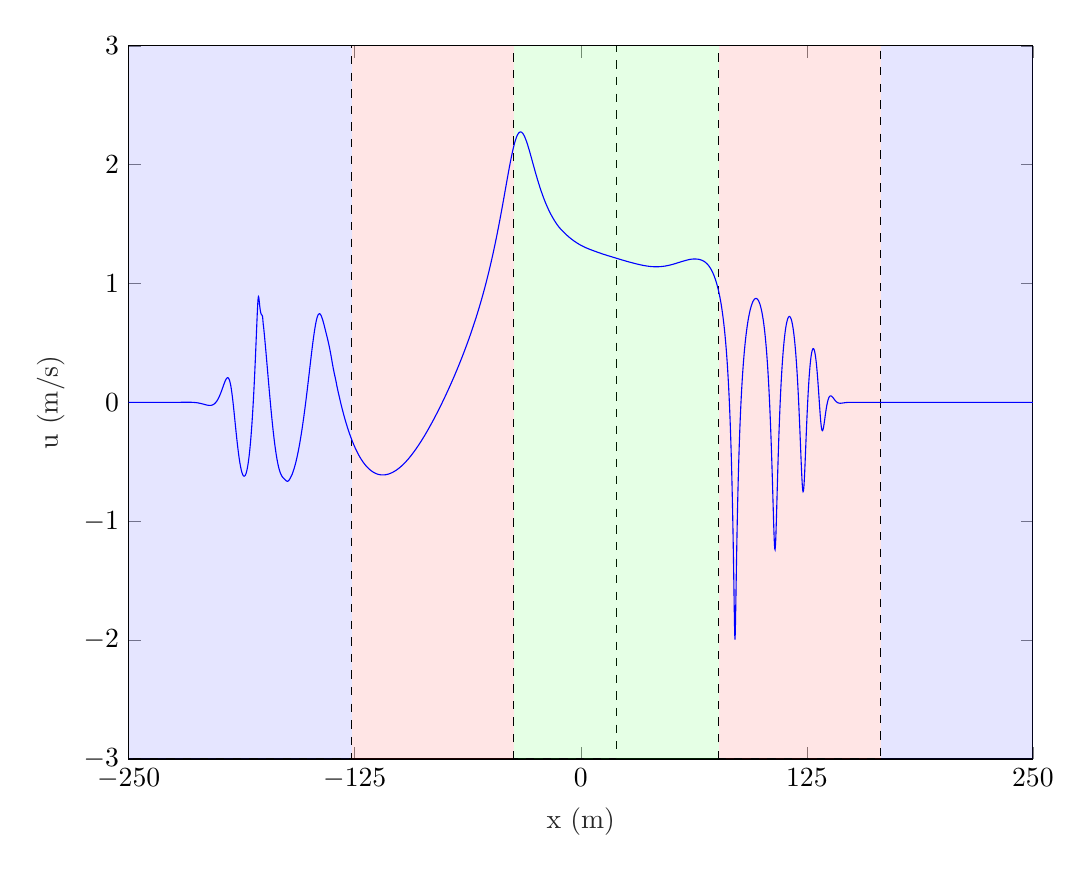
\begin{tikzpicture}

\begin{axis}[%
width=4.521in,
height=3.566in,
at={(0.758in,0.481in)},
scale only axis,
xmin=-250,
xmax=250,
xtick={-250, -125,    0,  125,  250},
xlabel style={font=\color{white!15!black}},
xlabel={x (m)},
ymin=-3,
ymax=3,
ytick={-3, -2, -1,  0,  1,  2,  3},
ylabel style={font=\color{white!15!black}},
ylabel={u (m/s)},
axis background/.style={fill=white}
]

\addplot[area legend, dashed, draw=black, fill=blue, fill opacity=0.1, forget plot]
table[row sep=crcr] {%
x	y\\
-250	-3\\
-250	3\\
-126.679671409596	3\\
-126.679671409596	-3\\
}--cycle;

\addplot[area legend, draw=none, fill=red, fill opacity=0.1, forget plot]
table[row sep=crcr] {%
x	y\\
-126.679671409596	-3\\
-126.679671409596	3\\
-37.0611924008642	3\\
-37.0611924008642	-3\\
}--cycle;

\addplot[area legend, dashed, draw=black, fill=green, fill opacity=0.1, forget plot]
table[row sep=crcr] {%
x	y\\
-37.0611924008642	-3\\
-37.0611924008642	3\\
19.5880540963537	3\\
19.5880540963537	-3\\
}--cycle;

\addplot[area legend, draw=none, fill=green, fill opacity=0.1, forget plot]
table[row sep=crcr] {%
x	y\\
19.5880540963537	-3\\
19.5880540963537	3\\
76.2373005935716	3\\
76.2373005935716	-3\\
}--cycle;

\addplot[area legend, dashed, draw=black, fill=red, fill opacity=0.1, forget plot]
table[row sep=crcr] {%
x	y\\
76.2373005935716	-3\\
76.2373005935716	3\\
165.855779602303	3\\
165.855779602303	-3\\
}--cycle;

\addplot[area legend, draw=none, fill=blue, fill opacity=0.1, forget plot]
table[row sep=crcr] {%
x	y\\
165.855779602303	-3\\
165.855779602303	3\\
250	3\\
250	-3\\
}--cycle;
\addplot [color=blue, forget plot]
  table[row sep=crcr]{%
-250.100003333444	0\\
-249.933331111037	5.07170710963883e-09\\
-249.76665888863	5.48096400950047e-09\\
-249.599986666222	6.15168177293456e-09\\
-249.433314443815	6.94703073586194e-09\\
-249.266642221407	7.726960048915e-09\\
-249.099969999	8.34399412607135e-09\\
-248.933297776593	8.64315906566177e-09\\
-248.766625554185	8.46205696500905e-09\\
-248.599953331778	7.63069557034928e-09\\
-248.43328110937	5.97165319876698e-09\\
-248.266608886963	3.29852690377259e-09\\
-248.099936664555	-5.75827261035383e-10\\
-247.933264442148	-5.8572822525782e-09\\
-247.766592219741	-1.27528218943048e-08\\
-247.599919997333	-2.14787984600834e-08\\
-247.433247774926	-3.22598163037557e-08\\
-247.266575552518	-4.53283144790442e-08\\
-247.099903330111	-6.09252835547121e-08\\
-246.933231107704	-7.93000970217044e-08\\
-246.766558885296	-1.00710725609112e-07\\
-246.599886662889	-1.25423992426339e-07\\
-246.433214440481	-1.53715458501072e-07\\
-246.266542218074	-1.85869581750941e-07\\
-246.099869995667	-2.22179960148238e-07\\
-245.933197773259	-2.62949425891521e-07\\
-245.766525550852	-3.0848995243668e-07\\
-245.599853328444	-3.59122925052474e-07\\
-245.433181106037	-4.15179139078758e-07\\
-245.266508883629	-4.76998777179831e-07\\
-245.099836661222	-5.44931409417307e-07\\
-244.933164438815	-6.19336114003391e-07\\
-244.766492216407	-7.00581381131388e-07\\
-244.599819994	-7.89045040297528e-07\\
-244.433147771592	-8.8511411539042e-07\\
-244.266475549185	-9.89184716280593e-07\\
-244.099803326778	-1.10166198555087e-06\\
-243.93313110437	-1.22295964484831e-06\\
-243.766458881963	-1.35349980318923e-06\\
-243.599786659555	-1.49371253170542e-06\\
-243.433114437148	-1.64403560133381e-06\\
-243.26644221474	-1.80491442442205e-06\\
-243.099769992333	-1.976800591234e-06\\
-242.933097769926	-2.16015198785481e-06\\
-242.766425547518	-2.35543222806825e-06\\
-242.599753325111	-2.56310930840506e-06\\
-242.433081102703	-2.78365534292374e-06\\
-242.266408880296	-3.01754540062056e-06\\
-242.099736657889	-3.26525652956372e-06\\
-241.933064435481	-3.52726667593518e-06\\
-241.766392213074	-3.8040533627188e-06\\
-241.599719990666	-4.09609250797817e-06\\
-241.433047768259	-4.40385695049082e-06\\
-241.266375545852	-4.72781474807265e-06\\
-241.099703323444	-5.06842760902874e-06\\
-240.933031101037	-5.42614896041553e-06\\
-240.766358878629	-5.80142192701465e-06\\
-240.599686656222	-6.19467738693992e-06\\
-240.433014433814	-6.60633148000119e-06\\
-240.266342211407	-7.03678320736693e-06\\
-240.099669989	-7.48641153601277e-06\\
-239.932997766592	-7.95557278999838e-06\\
-239.766325544185	-8.4445982401774e-06\\
-239.599653321777	-8.95379003485527e-06\\
-239.43298109937	-9.48341806798121e-06\\
-239.266308876963	-1.00337163222408e-05\\
-239.099636654555	-1.06048793975247e-05\\
-238.932964432148	-1.1197057798662e-05\\
-238.76629220974	-1.18103539482979e-05\\
-238.599619987333	-1.24448183226801e-05\\
-238.432947764926	-1.31004436768936e-05\\
-238.266275542518	-1.37771604318749e-05\\
-238.099603320111	-1.44748315414147e-05\\
-237.932931097703	-1.51932468757912e-05\\
-237.766258875296	-1.59321173345982e-05\\
-237.599586652888	-1.66910683469615e-05\\
-237.432914430481	-1.74696341714863e-05\\
-237.266242208074	-1.82672509556234e-05\\
-237.099569985666	-1.90832497873032e-05\\
-236.932897763259	-1.99168495538683e-05\\
-236.766225540851	-2.07671490014441e-05\\
-236.599553318444	-2.16331190325246e-05\\
-236.432881096037	-2.25135944618988e-05\\
-236.266208873629	-2.34072741814264e-05\\
-236.099536651222	-2.43126813217518e-05\\
-235.932864428814	-2.52281998865184e-05\\
-235.766192206407	-2.61520356692402e-05\\
-235.599519983999	-2.70822027550942e-05\\
-235.432847761592	-2.80165394369356e-05\\
-235.266175539185	-2.89526725884783e-05\\
-235.099503316777	-2.98880221282967e-05\\
-234.93283109437	-3.08197820632243e-05\\
-234.766158871962	-3.17449145588459e-05\\
-234.599486649555	-3.26601356501118e-05\\
-234.432814427148	-3.35619049732527e-05\\
-234.26614220474	-3.44464136972873e-05\\
-234.099469982333	-3.53095731470218e-05\\
-233.932797759925	-3.61470023854566e-05\\
-233.766125537518	-3.69540150022555e-05\\
-233.599453315111	-3.77256083140041e-05\\
-233.432781092703	-3.84564596989712e-05\\
-233.266108870296	-3.91410297499546e-05\\
-233.099436647888	-3.97731557674547e-05\\
-232.932764425481	-4.0346446547151e-05\\
-232.766092203073	-4.08541293244024e-05\\
-232.599419980666	-4.12890397365936e-05\\
-232.432747758259	-4.16436101533723e-05\\
-232.266075535851	-4.19098561515306e-05\\
-232.099403313444	-4.20793678434699e-05\\
-231.932731091036	-4.21432982476742e-05\\
-231.766058868629	-4.20923522082163e-05\\
-231.599386646222	-4.19167716758445e-05\\
-231.432714423814	-4.16063343153687e-05\\
-231.266042201407	-4.1150342131253e-05\\
-231.099369978999	-4.05376038785747e-05\\
-230.932697756592	-3.97564419359538e-05\\
-230.766025534184	-3.87946794155939e-05\\
-230.599353311777	-3.76396301980191e-05\\
-230.43268108937	-3.62781090735026e-05\\
-230.266008866962	-3.46964074913926e-05\\
-230.099336644555	-3.28803169649376e-05\\
-229.932664422147	-3.08151071765349e-05\\
-229.76599219974	-2.84855466853937e-05\\
-229.599319977333	-2.58758901107511e-05\\
-229.432647754925	-2.29699005283699e-05\\
-229.265975532518	-1.97508349865177e-05\\
-229.09930331011	-1.62014961889812e-05\\
-228.932631087703	-1.23042120478374e-05\\
-228.765958865296	-8.04083538052504e-06\\
-228.599286642888	-3.39281022719709e-06\\
-228.432614420481	1.65881952469466e-06\\
-228.265942198073	7.13342112633811e-06\\
-228.099269975666	1.30506980969418e-05\\
-227.932597753258	1.94306779114749e-05\\
-227.765925530851	2.62936726319461e-05\\
-227.599253308444	3.36602352307627e-05\\
-227.432581086036	4.15511195397848e-05\\
-227.265908863629	4.99872128515026e-05\\
-227.099236641221	5.89894981050894e-05\\
-226.932564418814	6.8578989241168e-05\\
-226.765892196407	7.87766578275237e-05\\
-226.599219973999	8.96033590147126e-05\\
-226.432547751592	0.000101079753958262\\
-226.265875529184	0.000113226226261459\\
-226.099203306777	0.000126062792125487\\
-225.932531084369	0.000139608996639281\\
-225.765858861962	0.000153883805673171\\
-225.599186639555	0.000168905498411857\\
-225.432514417147	0.000184691537207826\\
-225.26584219474	0.000201258430151782\\
-225.099169972332	0.000218621615071497\\
-224.932497749925	0.000236795290606111\\
-224.765825527518	0.000255792270766596\\
-224.59915330511	0.000275623808530335\\
-224.432481082703	0.000296299429066084\\
-224.265808860295	0.000317826744874953\\
-224.099136637888	0.000340211248447732\\
-223.932464415481	0.000363456095914833\\
-223.765792193073	0.000387561965629927\\
-223.599119970666	0.000412526785860878\\
-223.432447748258	0.000438345411955503\\
-223.265775525851	0.00046500948774914\\
-223.099103303443	0.000492507177016808\\
-222.932431081036	0.000520822856945388\\
-222.765758858629	0.000549936861080499\\
-222.599086636221	0.000579825179632529\\
-222.432414413814	0.000610459175283586\\
-222.265742191406	0.000641805254004568\\
-222.099069968999	0.000673824517022526\\
-221.932397746592	0.00070647247522271\\
-221.765725524184	0.000739698747554827\\
-221.599053301777	0.000773446670947608\\
-221.432381079369	0.000807652808272538\\
-221.265708856962	0.000842246785506175\\
-221.099036634554	0.000877150876124165\\
-220.932364412147	0.000912279515552372\\
-220.76569218974	0.00094753901479916\\
-220.599019967332	0.000982827149435956\\
-220.432347744925	0.00101803273412733\\
-220.265675522517	0.00105303525032443\\
-220.09900330011	0.00108770448016955\\
-219.932331077703	0.00112190005287101\\
-219.765658855295	0.0011554710932957\\
-219.598986632888	0.00118825580572386\\
-219.43231441048	0.00122008110423006\\
-219.265642188073	0.00125076224710966\\
-219.098969965666	0.00128010244670821\\
-218.932297743258	0.00130789252754222\\
-218.765625520851	0.00133391058393269\\
-218.598953298443	0.00135791603209579\\
-218.432281076036	0.0013796820955482\\
-218.265608853628	0.00139892908570255\\
-218.098936631221	0.00141538477725831\\
-217.932264408814	0.00142875829014915\\
-217.765592186406	0.00143874602008943\\
-217.598919963999	0.00144502912639331\\
-217.432247741591	0.00144727510180974\\
-217.265575519184	0.00144513600311026\\
-217.098903296777	0.00143825022875321\\
-216.932231074369	0.00142624116804016\\
-216.765558851962	0.00140871813346704\\
-216.598886629554	0.00138527621141566\\
-216.432214407147	0.00135549650744131\\
-216.26554218474	0.00131894695416707\\
-216.098869962332	0.00127518191695789\\
-215.932197739925	0.00122374365015396\\
-215.765525517517	0.00116416227455401\\
-215.59885329511	0.00109595663696823\\
-215.432181072702	0.00101863560637369\\
-215.265508850295	0.000931698294523086\\
-215.098836627888	0.000834635548027968\\
-214.93216440548	0.000726931454569311\\
-214.765492183073	0.000608064295641814\\
-214.598819960665	0.000477508201074975\\
-214.432147738258	0.000334734713396258\\
-214.265475515851	0.000179214620825734\\
-214.098803293443	1.04201988767299e-05\\
-213.932131071036	-0.000172172770595023\\
-213.765458848628	-0.000369082675458798\\
-213.598786626221	-0.000580819499517249\\
-213.432114403813	-0.000807882063281783\\
-213.265442181406	-0.00105075511170899\\
-213.098769958999	-0.00130990610368786\\
-212.932097736591	-0.00158578191791114\\
-212.765425514184	-0.00187880528534351\\
-212.598753291776	-0.00218937099714424\\
-212.432081069369	-0.00251784190471195\\
-212.265408846962	-0.00286454467089722\\
-212.098736624554	-0.00322976532115248\\
-211.932064402147	-0.00361374459527735\\
-211.765392179739	-0.00401667314890825\\
-211.598719957332	-0.00443868635039185\\
-211.432047734924	-0.00487985887734247\\
-211.265375512517	-0.0053402003853847\\
-211.09870329011	-0.00581965068246583\\
-210.932031067702	-0.00631806711190722\\
-210.765358845295	-0.00683522206383836\\
-210.598686622887	-0.00737080109710136\\
-210.43201440048	-0.00792439602210004\\
-210.265342178073	-0.00849549612698504\\
-210.098669955665	-0.00908347573527057\\
-209.931997733258	-0.00968759844393473\\
-209.76532551085	-0.0103070025539635\\
-209.598653288443	-0.0109406980021447\\
-209.431981066036	-0.0115875579757584\\
-209.265308843628	-0.0122463129714946\\
-209.098636621221	-0.0129155436250597\\
-208.931964398813	-0.0135936745961139\\
-208.765292176406	-0.0142789679164203\\
-208.598619953998	-0.0149695167111585\\
-208.431947731591	-0.015663239145947\\
-208.265275509184	-0.0163578725792377\\
-208.098603286776	-0.0170509682336909\\
-207.931931064369	-0.0177398861712076\\
-207.765258841961	-0.0184217904527995\\
-207.598586619554	-0.0190936452689329\\
-207.431914397147	-0.0197522103277828\\
-207.265242174739	-0.0203940383625807\\
-207.098569952332	-0.0210154730336693\\
-206.931897729924	-0.0216126462352915\\
-206.765225507517	-0.0221814768354531\\
-206.598553285109	-0.0227176715117101\\
-206.431881062702	-0.0232167240028115\\
-206.265208840295	-0.0236739166267699\\
-206.098536617887	-0.0240843254196402\\
-205.93186439548	-0.0244425792689101\\
-205.765192173072	-0.0247441903131799\\
-205.598519950665	-0.0249828598378723\\
-205.431847728258	-0.0251530653465029\\
-205.26517550585	-0.0252488891755759\\
-205.098503283443	-0.0252642724279298\\
-204.931831061035	-0.0251929822147213\\
-204.765158838628	-0.0250286375508477\\
-204.598486616221	-0.0247647274760646\\
-204.431814393813	-0.024394617375455\\
-204.265142171406	-0.0239115667282336\\
-204.098469948998	-0.0233087518187673\\
-203.931797726591	-0.0225792812685353\\
-203.765125504183	-0.0217162192144513\\
-203.598453281776	-0.0207126079991276\\
-203.431781059369	-0.0195614944627088\\
-203.265108836961	-0.0182559568095995\\
-203.098436614554	-0.0167891335696735\\
-202.931764392146	-0.0151542554357925\\
-202.765092169739	-0.0133446796502739\\
-202.598419947332	-0.0113539264413492\\
-202.431747724924	-0.00917571766451615\\
-202.265075502517	-0.00680401854516531\\
-202.098403280109	-0.00423308149033984\\
-201.931731057702	-0.00145749556079596\\
-201.765058835294	0.00152776325168176\\
-201.598386612887	0.00472727848134152\\
-201.43171439048	0.00814513489634709\\
-201.265042168072	0.0117848537089014\\
-201.098369945665	0.0156493276917092\\
-200.931697723257	0.0197407516135238\\
-200.76502550085	0.0240605439559086\\
-200.598353278443	0.0286092664406641\\
-200.431681056035	0.0333865361008993\\
-200.265008833628	0.0383909249456232\\
-200.09833661122	0.043619860972589\\
-199.931664388813	0.0490695349058952\\
-199.764992166406	0.0547347903641302\\
-199.598319943998	0.0606089898419335\\
-199.431647721591	0.0666838775164182\\
-199.264975499183	0.0729494536069869\\
-199.098303276776	0.0793938313375502\\
-198.931631054368	0.0860030803993503\\
-198.764958831961	0.092761058777989\\
-198.598286609554	0.0996492489184387\\
-198.431614387146	0.106646578898418\\
-198.264942164739	0.11372923399035\\
-198.098269942331	0.120870470237678\\
-197.931597719924	0.128040418410539\\
-197.764925497517	0.135205889444677\\
-197.598253275109	0.142330179189629\\
-197.431581052702	0.149372886277793\\
-197.264908830294	0.156289731697655\\
-197.098236607887	0.163032402792329\\
-196.93156438548	0.169548427136353\\
-196.764892163072	0.17578107654335\\
-196.598219940665	0.181669321532444\\
-196.431547718257	0.187147874887503\\
-196.26487549585	0.192147258035383\\
-196.098203273442	0.1965940327984\\
-195.931531051035	0.200410945783509\\
-195.764858828628	0.203517847525129\\
-195.59818660622	0.205827544356823\\
-195.431514383813	0.207268910978317\\
-195.264842161405	0.207743987648504\\
-195.098169938998	0.207172479498836\\
-194.931497716591	0.205471048258343\\
-194.764825494183	0.202560920321822\\
-194.598153271776	0.198368930784441\\
-194.431481049368	0.192829675741247\\
-194.264808826961	0.185887567511973\\
-194.098136604553	0.177498915883097\\
-193.931464382146	0.167634029150741\\
-193.764792159739	0.156278819700837\\
-193.598119937331	0.143436212431091\\
-193.431447714924	0.129126986318049\\
-193.264775492516	0.113389989855373\\
-193.098103270109	0.0962818498980174\\
-192.931431047702	0.0778759931812276\\
-192.764758825294	0.0582610121085721\\
-192.598086602887	0.0375386968427054\\
-192.431414380479	0.0158215393924826\\
-192.264742158072	-0.00676999102396642\\
-192.098069935665	-0.0301098584507515\\
-191.931397713257	-0.054069270843986\\
-191.76472549085	-0.0785189360138838\\
-191.598053268442	-0.103331260288128\\
-191.431381046035	-0.128382072804896\\
-191.264708823627	-0.153552061340735\\
-191.09803660122	-0.178727846707798\\
-190.931364378813	-0.203802719085366\\
-190.764692156405	-0.228677080208616\\
-190.598019933998	-0.253258632780457\\
-190.43134771159	-0.277462421215676\\
-190.264675489183	-0.301210717207714\\
-190.098003266776	-0.324432726729846\\
-189.931331044368	-0.34706420116118\\
-189.764658821961	-0.369046985797761\\
-189.597986599553	-0.390328605185912\\
-189.431314377146	-0.410861846335264\\
-189.264642154738	-0.430604265808944\\
-189.097969932331	-0.449517727715501\\
-188.931297709924	-0.467567964267633\\
-188.764625487516	-0.484724164637293\\
-188.597953265109	-0.500958526316267\\
-188.431281042701	-0.516245996186856\\
-188.264608820294	-0.530563818286503\\
-188.097936597887	-0.543891293272248\\
-187.931264375479	-0.556209452673396\\
-187.764592153072	-0.567500800710247\\
-187.597919930664	-0.577749072094253\\
-187.431247708257	-0.586938999670401\\
-187.26457548585	-0.595056115104788\\
-187.097903263442	-0.602086567912925\\
-186.931231041035	-0.608016952755761\\
-186.764558818627	-0.612834153363413\\
-186.59788659622	-0.616525205630162\\
-186.431214373812	-0.61908273890048\\
-186.264542151405	-0.620477211597238\\
-186.097869928998	-0.620711948585773\\
-185.93119770659	-0.61976766087709\\
-185.764525484183	-0.617630246999707\\
-185.597853261775	-0.614285205798894\\
-185.431181039368	-0.609717411424345\\
-185.264508816961	-0.603910987675766\\
-185.097836594553	-0.596849390361794\\
-184.931164372146	-0.588515263880421\\
-184.764492149738	-0.578890268918878\\
-184.597819927331	-0.567955173263076\\
-184.431147704923	-0.555689781737276\\
-184.264475482516	-0.542072750874591\\
-184.097803260109	-0.527081662455323\\
-183.931131037701	-0.510693018531906\\
-183.764458815294	-0.492882056126857\\
-183.597786592886	-0.473622816163028\\
-183.431114370479	-0.45288818648335\\
-183.264442148072	-0.430649764021856\\
-183.097769925664	-0.406877913841365\\
-182.931097703257	-0.381541902623515\\
-182.764425480849	-0.354609849748658\\
-182.597753258442	-0.326048791747659\\
-182.431081036035	-0.295824915485898\\
-182.264408813627	-0.263903653654635\\
-182.09773659122	-0.230249885353919\\
-181.931064368812	-0.194828379721184\\
-181.764392146405	-0.157604233212463\\
-181.597719923997	-0.11854337289256\\
-181.43104770159	-0.0776134023409721\\
-181.264375479183	-0.0347847387448765\\
-181.097703256775	0.0099680645265111\\
-180.931031034368	0.0566643773635268\\
-180.76435881196	0.105314927407814\\
-180.597686589553	0.155918469848633\\
-180.431014367146	0.20845706547523\\
-180.264342144738	0.262889519197335\\
-180.097669922331	0.319142366962614\\
-179.930997699923	0.377096830534325\\
-179.764325477516	0.436569540931937\\
-179.597653255108	0.49728389599033\\
-179.430981032701	0.558826001154758\\
-179.264308810294	0.620574859821035\\
-179.097636587886	0.681589599895053\\
-178.930964365479	0.740424924032036\\
-178.764292143071	0.794835438614219\\
-178.597619920664	0.841361850967204\\
-178.430947698257	0.875056883790948\\
-178.264275475849	0.890552426183976\\
-178.097603253442	0.886145718867681\\
-177.930931031034	0.867113203868992\\
-177.764258808627	0.842967842209028\\
-177.59758658622	0.818699774013041\\
-177.430914363812	0.796717789341262\\
-177.264242141405	0.778048383951367\\
-177.097569918997	0.763034538043716\\
-176.93089769659	0.751663296256806\\
-176.764225474182	0.743700430334087\\
-176.597553251775	0.738688536415788\\
-176.430881029368	0.735833516278698\\
-176.26420880696	0.733646473537485\\
-176.097536584553	0.728922313719639\\
-175.930864362145	0.714686000288236\\
-175.764192139738	0.684461846803206\\
-175.597519917331	0.655293829745117\\
-175.430847694923	0.638352335427009\\
-175.264175472516	0.613774132520637\\
-175.097503250108	0.586569850557533\\
-174.930831027701	0.560967481003605\\
-174.764158805294	0.534419086620299\\
-174.597486582886	0.506553277532194\\
-174.430814360479	0.478721419786308\\
-174.264142138071	0.450368564068568\\
-174.097469915664	0.421536422868522\\
-173.930797693256	0.392533314765361\\
-173.764125470849	0.363271888844228\\
-173.597453248442	0.333842177115698\\
-173.430781026034	0.304339048163248\\
-173.264108803627	0.274776577681639\\
-173.097436581219	0.24521730079633\\
-172.930764358812	0.215714856871131\\
-172.764092136405	0.186306068039832\\
-172.597419913997	0.157036958927439\\
-172.43074769159	0.127948138467719\\
-172.264075469182	0.0990772358474814\\
-172.097403246775	0.0704611189275139\\
-171.930731024367	0.042135074922605\\
-171.76405880196	0.0141331316746898\\
-171.597386579553	-0.0135127230107727\\
-171.430714357145	-0.0407718519950572\\
-171.264042134738	-0.067615044898187\\
-171.09736991233	-0.0940140692838618\\
-170.930697689923	-0.11994228809076\\
-170.764025467516	-0.14537420101717\\
-170.597353245108	-0.170285517603652\\
-170.430681022701	-0.194653295985079\\
-170.264008800293	-0.218455920936238\\
-170.097336577886	-0.241673014523751\\
-169.930664355479	-0.264285563031716\\
-169.763992133071	-0.286276063539721\\
-169.597319910664	-0.307628146747997\\
-169.430647688256	-0.328326787085436\\
-169.263975465849	-0.348358402807163\\
-169.097303243441	-0.367710726006014\\
-168.930631021034	-0.386372925188392\\
-168.763958798627	-0.404335621150963\\
-168.597286576219	-0.421590747204318\\
-168.430614353812	-0.438131753181773\\
-168.263942131404	-0.453953580488453\\
-168.097269908997	-0.469052570900268\\
-167.93059768659	-0.48342671811602\\
-167.763925464182	-0.497075533437538\\
-167.597253241775	-0.510000422364661\\
-167.430581019367	-0.522204494583529\\
-167.26390879696	-0.533692699842198\\
-167.097236574552	-0.544472119973511\\
-166.930564352145	-0.554551873919938\\
-166.763892129738	-0.563943497099227\\
-166.59721990733	-0.572661007934276\\
-166.430547684923	-0.580721454960857\\
-166.263875462515	-0.588144754121212\\
-166.097203240108	-0.594953976037959\\
-165.930531017701	-0.601175444707994\\
-165.763858795293	-0.606839361270271\\
-165.597186572886	-0.611979760601827\\
-165.430514350478	-0.616634937085337\\
-165.263842128071	-0.62084717375738\\
-165.097169905664	-0.624662914399253\\
-164.930497683256	-0.62813227007971\\
-164.763825460849	-0.631308479916388\\
-164.597153238441	-0.634246901757412\\
-164.430481016034	-0.637003178701641\\
-164.263808793626	-0.639631369604471\\
-164.097136571219	-0.642180523305163\\
-163.930464348812	-0.644690480939292\\
-163.763792126404	-0.647187187588429\\
-163.597119903997	-0.649676929560389\\
-163.430447681589	-0.652145428917565\\
-163.263775459182	-0.654555320558667\\
-163.097103236775	-0.656845244370606\\
-162.930431014367	-0.658936767764186\\
-162.76375879196	-0.660740613850964\\
-162.597086569552	-0.662163032406315\\
-162.430414347145	-0.663114936888481\\
-162.263742124737	-0.663521274397155\\
-162.09706990233	-0.663313064875117\\
-161.930397679923	-0.662455941151706\\
-161.763725457515	-0.66092548724161\\
-161.597053235108	-0.658717865693583\\
-161.4303810127	-0.655853551673621\\
-161.263708790293	-0.652378395534361\\
-161.097036567886	-0.648365834994033\\
-160.930364345478	-0.643917447819885\\
-160.763692123071	-0.639160464055868\\
-160.597019900663	-0.634237996938938\\
-160.430347678256	-0.629287681001668\\
-160.263675455848	-0.624401500393669\\
-160.097003233441	-0.619570134549209\\
-159.930331011034	-0.614672233164566\\
-159.763658788626	-0.60948654961497\\
-159.596986566219	-0.603764067075656\\
-159.430314343811	-0.59736801755018\\
-159.263642121404	-0.590343448579403\\
-159.096969898997	-0.582854540669136\\
-158.930297676589	-0.575089330452597\\
-158.763625454182	-0.567156532914627\\
-158.596953231774	-0.559040139354404\\
-158.430281009367	-0.550672779379473\\
-158.26360878696	-0.542007604902278\\
-158.096936564552	-0.53302497086084\\
-157.930264342145	-0.523706672959928\\
-157.763592119737	-0.514033906039642\\
-157.59691989733	-0.50400223415527\\
-157.430247674922	-0.493627166591403\\
-157.263575452515	-0.482927868891151\\
-157.096903230108	-0.471912661138055\\
-156.9302310077	-0.460581284941561\\
-156.763558785293	-0.448931840110227\\
-156.596886562885	-0.436962570222244\\
-156.430214340478	-0.42467071286576\\
-156.263542118071	-0.412054051583984\\
-156.096869895663	-0.399111179107477\\
-155.930197673256	-0.385841220973543\\
-155.763525450848	-0.372244486641729\\
-155.596853228441	-0.358322064304891\\
-155.430181006034	-0.344076012893469\\
-155.263508783626	-0.329508531712988\\
-155.096836561219	-0.314622466460679\\
-154.930164338811	-0.299420640348879\\
-154.763492116404	-0.283906206007148\\
-154.596819893996	-0.268082265134169\\
-154.430147671589	-0.251952013038062\\
-154.263475449182	-0.235518584575529\\
-154.096803226774	-0.218784904668193\\
-153.930131004367	-0.201754272252377\\
-153.763458781959	-0.184429789457618\\
-153.596786559552	-0.166814883123096\\
-153.430114337145	-0.148912807805527\\
-153.263442114737	-0.130727682652816\\
-153.09676989233	-0.112263509328874\\
-152.930097669922	-0.0935250211692156\\
-152.763425447515	-0.0745175081178093\\
-152.596753225107	-0.055246839649759\\
-152.4300810027	-0.0357197735999072\\
-152.263408780293	-0.0159437083804308\\
-152.096736557885	0.00407282214310367\\
-151.930064335478	0.0243205394230677\\
-151.76339211307	0.0447887982821598\\
-151.596719890663	0.0654661747511356\\
-151.430047668256	0.0863396339586696\\
-151.263375445848	0.107395216999447\\
-151.096703223441	0.128617402988613\\
-150.930031001033	0.149989531905057\\
-150.763358778626	0.171493155488348\\
-150.596686556219	0.193108702263779\\
-150.430014333811	0.214814726079406\\
-150.263342111404	0.236588372925382\\
-150.096669888996	0.258404911645198\\
-149.929997666589	0.280238053043569\\
-149.763325444181	0.302059374955557\\
-149.596653221774	0.32383860059635\\
-149.429980999367	0.345543514479375\\
-149.263308776959	0.367140101685727\\
-149.096636554552	0.388592095390089\\
-148.929964332144	0.409860989907756\\
-148.763292109737	0.430906281265108\\
-148.59661988733	0.451685500283284\\
-148.429947664922	0.472154218212035\\
-148.263275442515	0.492265838086075\\
-148.096603220107	0.511972163247712\\
-147.9299309977	0.531223189107064\\
-147.763258775293	0.549967604527996\\
-147.596586552885	0.568152987649415\\
-147.429914330478	0.585726218666241\\
-147.26324210807	0.602633481386172\\
-147.096569885663	0.618821027452742\\
-146.929897663255	0.634235660612455\\
-146.763225440848	0.648825209153237\\
-146.596553218441	0.662539101663393\\
-146.429880996033	0.675329578304322\\
-146.263208773626	0.687151771459252\\
-146.096536551218	0.697964495597879\\
-145.929864328811	0.707730893784113\\
-145.763192106404	0.716419756205821\\
-145.596519883996	0.724005700130118\\
-145.429847661589	0.730470132723917\\
-145.263175439181	0.735801372878608\\
-145.096503216774	0.739995642907716\\
-144.929830994366	0.743056930959002\\
-144.763158771959	0.744997464621914\\
-144.596486549552	0.745837602873495\\
-144.429814327144	0.745605685053092\\
-144.263142104737	0.744339135112702\\
-144.096469882329	0.74207469195174\\
-143.929797659922	0.738867847125867\\
-143.763125437515	0.734772532370907\\
-143.596453215107	0.7298487745186\\
-143.4297809927	0.724160092404897\\
-143.263108770292	0.717772700368201\\
-143.096436547885	0.710754191907484\\
-142.929764325477	0.703172631397376\\
-142.76309210307	0.695095191047417\\
-142.596419880663	0.686587467209072\\
-142.429747658255	0.677712162058817\\
-142.263075435848	0.668528516411681\\
-142.09640321344	0.659091176965899\\
-141.929730991033	0.649449810912554\\
-141.763058768626	0.639648174105077\\
-141.596386546218	0.629723892835923\\
-141.429714323811	0.619707724895718\\
-141.263042101403	0.609623520609554\\
-141.096369878996	0.599487742866914\\
-140.929697656589	0.589309568253969\\
-140.763025434181	0.579090554137481\\
-140.596353211774	0.568825046833739\\
-140.429680989366	0.558499953904562\\
-140.263008766959	0.548095496592719\\
-140.096336544551	0.53758538736989\\
-139.929664322144	0.526937871143753\\
-139.762992099737	0.516116496532369\\
-139.596319877329	0.505081654782597\\
-139.429647654922	0.49379196792599\\
-139.262975432514	0.482206643125017\\
-139.096303210107	0.470287742132366\\
-138.9296309877	0.458003380427707\\
-138.762958765292	0.445330572461471\\
-138.596286542885	0.432258975325238\\
-138.429614320477	0.418793829797189\\
-138.26294209807	0.404959349627714\\
-138.096269875663	0.39080034518777\\
-137.929597653255	0.376383210858115\\
-137.762925430848	0.361794759260146\\
-137.59625320844	0.347139334960874\\
-137.429580986033	0.332533376470786\\
-137.262908763625	0.31809851836061\\
-137.096236541218	0.303952442016898\\
-136.929564318811	0.290198845143836\\
-136.762892096403	0.276916870165317\\
-136.596219873996	0.264150649277499\\
-136.429547651588	0.251896760149993\\
-136.262875429181	0.240096609022761\\
-136.096203206774	0.228626942876055\\
-135.929530984366	0.217298059099484\\
-135.762858761959	0.205867583798404\\
-135.596186539551	0.194083922299795\\
-135.429514317144	0.181768172347836\\
-135.262842094736	0.168913331129692\\
-135.096169872329	0.155723150695102\\
-134.929497649922	0.142568627857138\\
-134.762825427514	0.129770037428308\\
-134.596153205107	0.117437505790277\\
-134.429480982699	0.105544435344122\\
-134.262808760292	0.0940413384972912\\
-134.096136537885	0.0828439398656952\\
-133.929464315477	0.0718455365822703\\
-133.76279209307	0.0609409428546852\\
-133.596119870662	0.0500377952319502\\
-133.429447648255	0.0390867577465892\\
-133.262775425848	0.0280916561633614\\
-133.09610320344	0.0170989625934955\\
-132.929430981033	0.006185143745379\\
-132.762758758625	-0.00457141476312277\\
-132.596086536218	-0.0151246131819681\\
-132.42941431381	-0.0254702925362922\\
-132.262742091403	-0.0356312796072209\\
-132.096069868996	-0.045641182221785\\
-131.929397646588	-0.0555402225282184\\
-131.762725424181	-0.0653561772718037\\
-131.596053201773	-0.075098769446357\\
-131.429380979366	-0.0847596328703288\\
-131.262708756959	-0.0943195874280204\\
-131.096036534551	-0.103759527552823\\
-130.929364312144	-0.113067087149711\\
-130.762692089736	-0.122238291863009\\
-130.596019867329	-0.131277074507723\\
-130.429347644921	-0.140192889616399\\
-130.262675422514	-0.148996384590963\\
-130.096003200107	-0.15769526239811\\
-129.929330977699	-0.166292180278108\\
-129.762658755292	-0.174785279317052\\
-129.595986532884	-0.183170075795289\\
-129.429314310477	-0.191442898691167\\
-129.26264208807	-0.199603110170149\\
-129.095969865662	-0.207653630470361\\
-128.929297643255	-0.215599190980392\\
-128.762625420847	-0.223444507982341\\
-128.59595319844	-0.231192668659711\\
-128.429280976033	-0.238844978978138\\
-128.262608753625	-0.246401299065937\\
-128.095936531218	-0.253860705770567\\
-127.92926430881	-0.261221952961381\\
-127.762592086403	-0.268484082842469\\
-127.595919863995	-0.275646979412832\\
-127.429247641588	-0.282710962750696\\
-127.262575419181	-0.289676632755242\\
-127.095903196773	-0.296544523258437\\
-126.929230974366	-0.303315062875934\\
-126.762558751958	-0.309989027090714\\
-126.595886529551	-0.316567467812678\\
-126.429214307144	-0.323051644237195\\
-126.262542084736	-0.329443182119675\\
-126.095869862329	-0.335743611848344\\
-125.929197639921	-0.341954127989261\\
-125.762525417514	-0.348075816475166\\
-125.595853195106	-0.354109679685017\\
-125.429180972699	-0.360056579729593\\
-125.262508750292	-0.365917332696184\\
-125.095836527884	-0.371692794340388\\
-124.929164305477	-0.377383635602798\\
-124.762492083069	-0.382990136947975\\
-124.595819860662	-0.388512330114062\\
-124.429147638255	-0.393950215615269\\
-124.262475415847	-0.399303996449114\\
-124.09580319344	-0.404574303850989\\
-123.929130971032	-0.409762182506359\\
-123.762458748625	-0.414868998864297\\
-123.595786526218	-0.419896159647532\\
-123.42911430381	-0.424844843423489\\
-123.262442081403	-0.429715681626966\\
-123.095769858995	-0.434508775922039\\
-122.929097636588	-0.439223960463216\\
-122.76242541418	-0.443861158245202\\
-122.595753191773	-0.448420710377958\\
-122.429080969366	-0.452903470257875\\
-122.262408746958	-0.457310702738196\\
-122.095736524551	-0.461643714370508\\
-121.929064302143	-0.465903588886892\\
-121.762392079736	-0.470091004062765\\
-121.595719857329	-0.474206174898828\\
-121.429047634921	-0.478249209799827\\
-121.262375412514	-0.482220375433562\\
-121.095703190106	-0.486120150065095\\
-120.929030967699	-0.489949264372668\\
-120.762358745291	-0.49370853238608\\
-120.595686522884	-0.497398698449629\\
-120.429014300477	-0.50102033942854\\
-120.262342078069	-0.504573841511869\\
-120.095669855662	-0.508059543388206\\
-119.928997633254	-0.511477891338786\\
-119.762325410847	-0.51482945373835\\
-119.59565318844	-0.518114884558649\\
-119.428980966032	-0.521334873448029\\
-119.262308743625	-0.524490004656595\\
-119.095636521217	-0.527580694131123\\
-118.92896429881	-0.530607300812398\\
-118.762292076403	-0.533570226183177\\
-118.595619853995	-0.536469897994126\\
-118.428947631588	-0.539306778639265\\
-118.26227540918	-0.54208136371117\\
-118.095603186773	-0.544794167936071\\
-117.928930964365	-0.547445677792908\\
-117.762258741958	-0.550036295883232\\
-117.595586519551	-0.552566459971998\\
-117.428914297143	-0.555036603409436\\
-117.262242074736	-0.557447141232718\\
-117.095569852328	-0.559798572038998\\
-116.928897629921	-0.562091359564183\\
-116.762225407514	-0.564325959407348\\
-116.595553185106	-0.566502778463785\\
-116.428880962699	-0.568622116218735\\
-116.262208740291	-0.570684298423015\\
-116.095536517884	-0.572689714275304\\
-115.928864295477	-0.574638900274833\\
-115.762192073069	-0.576532360053185\\
-115.595519850662	-0.578370348862792\\
-115.428847628254	-0.5801531847885\\
-115.262175405847	-0.581881251333397\\
-115.095503183439	-0.583554867217606\\
-114.928830961032	-0.585174347674155\\
-114.762158738625	-0.586739876362843\\
-114.595486516217	-0.588251662612426\\
-114.42881429381	-0.589710018307645\\
-114.262142071402	-0.591115395001752\\
-114.095469848995	-0.592468246783259\\
-113.928797626588	-0.59376892137844\\
-113.76212540418	-0.595017817525438\\
-113.595453181773	-0.596215375293863\\
-113.428780959365	-0.597361901511875\\
-113.262108736958	-0.598457594833011\\
-113.09543651455	-0.599502710507115\\
-112.928764292143	-0.600497570642302\\
-112.762092069736	-0.601442456118092\\
-112.595419847328	-0.602337576557445\\
-112.428747624921	-0.603183150391836\\
-112.262075402513	-0.603979497544702\\
-112.095403180106	-0.604726881343561\\
-111.928730957699	-0.605425500077407\\
-111.762058735291	-0.606075561849456\\
-111.595386512884	-0.60667730798353\\
-111.428714290476	-0.607230926281893\\
-111.262042068069	-0.60773663071067\\
-111.095369845662	-0.6081948582605\\
-110.928697623254	-0.608605918149155\\
-110.762025400847	-0.608970090952486\\
-110.595353178439	-0.609287684461401\\
-110.428680956032	-0.609558893648817\\
-110.262008733624	-0.609783873085696\\
-110.095336511217	-0.609962904408278\\
-109.92866428881	-0.610096283209597\\
-109.761992066402	-0.610184368429926\\
-109.595319843995	-0.610227582711708\\
-109.428647621587	-0.610226337710933\\
-109.26197539918	-0.610181025562183\\
-109.095303176773	-0.610091966879581\\
-108.928630954365	-0.609959370499818\\
-108.761958731958	-0.609783395958991\\
-108.59528650955	-0.609563980099539\\
-108.428614287143	-0.609301510090721\\
-108.261942064735	-0.608995849996808\\
-108.095269842328	-0.608647499800744\\
-107.928597619921	-0.608256943979472\\
-107.761925397513	-0.607824817570298\\
-107.595253175106	-0.607351738920293\\
-107.428580952698	-0.606838214582716\\
-107.261908730291	-0.606284589195973\\
-107.095236507884	-0.605691113982898\\
-106.928564285476	-0.605057998622558\\
-106.761892063069	-0.604385267159425\\
-106.595219840661	-0.603673009087671\\
-106.428547618254	-0.60292139568579\\
-106.261875395847	-0.602130733229039\\
-106.095203173439	-0.601301357421817\\
-105.928530951032	-0.600433688981217\\
-105.761858728624	-0.599528088951119\\
-105.595186506217	-0.59858481267553\\
-105.428514283809	-0.597604210625049\\
-105.261842061402	-0.596586505892118\\
-105.095169838995	-0.595531551534548\\
-104.928497616587	-0.594439698036259\\
-104.76182539418	-0.593311991156263\\
-104.595153171772	-0.592149077726763\\
-104.428480949365	-0.590951108828597\\
-104.261808726958	-0.589718284328499\\
-104.09513650455	-0.588450699810509\\
-103.928464282143	-0.587148023634249\\
-103.761792059735	-0.585809860276755\\
-103.595119837328	-0.58443597817561\\
-103.42844761492	-0.583026380278682\\
-103.261775392513	-0.581581014288887\\
-103.095103170106	-0.580100323530249\\
-102.928430947698	-0.578583995484381\\
-102.761758725291	-0.577032744387077\\
-102.595086502883	-0.575446560876245\\
-102.428414280476	-0.573824196352689\\
-102.261742058069	-0.572166943452219\\
-102.095069835661	-0.570477302542354\\
-101.928397613254	-0.568754573460835\\
-101.761725390846	-0.566997612582\\
-101.595053168439	-0.565206332600976\\
-101.428380946032	-0.563380994653852\\
-101.261708723624	-0.561521416664803\\
-101.095036501217	-0.559626031186537\\
-100.928364278809	-0.557695134989869\\
-100.761692056402	-0.55573097175193\\
-100.595019833994	-0.553735045051426\\
-100.428347611587	-0.551707447676535\\
-100.26167538918	-0.549647664936293\\
-100.095003166772	-0.547554979871467\\
-99.9283309443648	-0.545429126108925\\
-99.7616587219574	-0.543270491185634\\
-99.59498649955	-0.541079689725023\\
-99.4283142771426	-0.538857091583728\\
-99.2616420547351	-0.536602713535336\\
-99.0949698323277	-0.534316731977074\\
-98.9282976099203	-0.531999526838998\\
-98.7616253875129	-0.529651664965807\\
-98.5949531651055	-0.527273294540175\\
-98.4282809426981	-0.524863739767001\\
-98.2616087202907	-0.522423122684612\\
-98.0949364978833	-0.519952162008802\\
-97.9282642754758	-0.517450270027055\\
-97.7615920530684	-0.514917588386848\\
-97.594919830661	-0.512354880852159\\
-97.4282476082536	-0.509761642905936\\
-97.2615753858462	-0.507138334786929\\
-97.0949031634388	-0.504485572178288\\
-96.9282309410314	-0.501802989687294\\
-96.7615587186239	-0.499091321065293\\
-96.5948864962165	-0.496350681425776\\
-96.4282142738091	-0.493581057977254\\
-96.2615420514017	-0.49078321197747\\
-96.0948698289943	-0.487956744650344\\
-95.9281976065869	-0.485101866685665\\
-95.7615253841795	-0.482218799539018\\
-95.5948531617721	-0.479307195328302\\
-95.4281809393646	-0.476367593371623\\
-95.2615087169572	-0.473399904308088\\
-95.0948364945498	-0.470404282048392\\
-94.9281642721424	-0.467381168308649\\
-94.761492049735	-0.464330379522146\\
-94.5948198273276	-0.461252136220691\\
-94.4281476049202	-0.45814635732704\\
-94.2614753825127	-0.455012841502682\\
-94.0948031601053	-0.451851815318987\\
-93.9281309376979	-0.448663189688372\\
-93.7614587152905	-0.445447016902214\\
-93.5947864928831	-0.442203606525602\\
-93.4281142704757	-0.438932881287064\\
-93.2614420480683	-0.435634964269561\\
-93.0947698256608	-0.432310006832082\\
-92.9280976032534	-0.428957953018139\\
-92.761425380846	-0.425579021452482\\
-92.5947531584386	-0.422173421678109\\
-92.4280809360312	-0.418741221817203\\
-92.2614087136238	-0.415282442561081\\
-92.0947364912164	-0.411797131896444\\
-91.928064268809	-0.40828599117373\\
-91.7613920464015	-0.404748380401469\\
-91.5947198239941	-0.401185716349517\\
-91.4280476015867	-0.397598742245679\\
-91.2613753791793	-0.393984545576463\\
-91.0947031567719	-0.39034815824183\\
-90.9280309343645	-0.386698447017314\\
-90.7613587119571	-0.383036258402529\\
-90.5946864895496	-0.379356466545995\\
-90.4280142671422	-0.375654835655954\\
-90.2613420447348	-0.37192990099054\\
-90.0946698223274	-0.36818139457477\\
-89.92799759992	-0.364409255636362\\
-89.7613253775126	-0.360613487603403\\
-89.5946531551052	-0.356794187977067\\
-89.4279809326977	-0.352951711665938\\
-89.2613087102903	-0.349086744622632\\
-89.0946364878829	-0.345200144344771\\
-88.9279642654755	-0.341292846376519\\
-88.7612920430681	-0.337365590747698\\
-88.5946198206607	-0.333418874021168\\
-88.4279475982533	-0.329452907439888\\
-88.2612753758459	-0.325467768971174\\
-88.0946031534384	-0.321463600004911\\
-87.927930931031	-0.317440793627246\\
-87.7612587086236	-0.313399938943715\\
-87.5945864862162	-0.309341614388825\\
-87.4279142638088	-0.305266001011314\\
-87.2612420414014	-0.301172554497956\\
-87.094569818994	-0.297059940618329\\
-86.9278975965865	-0.292926217079049\\
-86.7612253741791	-0.288769248066917\\
-86.5945531517717	-0.284587205643378\\
-86.4278809293643	-0.280378946442274\\
-86.2612087069569	-0.276144081302277\\
-86.0945364845495	-0.271882907270801\\
-85.9278642621421	-0.267596240852038\\
-85.7611920397347	-0.263285160715792\\
-85.5945198173272	-0.25895078483206\\
-85.4278475949198	-0.254594069046414\\
-85.2611753725124	-0.250215681526748\\
-85.094503150105	-0.245816098841422\\
-84.9278309276976	-0.241395923347737\\
-84.7611587052902	-0.236956262719659\\
-84.5944864828828	-0.232498895196182\\
-84.4278142604753	-0.228026131454273\\
-84.2611420380679	-0.223540329885723\\
-84.0944698156605	-0.219043282161877\\
-83.9277975932531	-0.214535779732371\\
-83.7611253708457	-0.210017523353872\\
-83.5944531484383	-0.205487406497528\\
-83.4277809260309	-0.200943885731546\\
-83.2611087036234	-0.196385240413188\\
-83.094436481216	-0.191809766155081\\
-82.9277642588086	-0.187215920409921\\
-82.7610920364012	-0.182602519219206\\
-82.5944198139938	-0.177968961950718\\
-82.4277475915864	-0.173315395191059\\
-82.261075369179	-0.168642637073658\\
-82.0944031467716	-0.163951791262646\\
-81.9277309243641	-0.159243730596015\\
-81.7610587019567	-0.154518773375306\\
-81.5943864795493	-0.14977666385859\\
-81.4277142571419	-0.145016873939852\\
-81.2610420347345	-0.140239069826376\\
-81.0943698123271	-0.135443403770182\\
-80.9276975899197	-0.130630504827999\\
-80.7610253675122	-0.125801179415794\\
-80.5943531451048	-0.120956121495291\\
-80.4276809226974	-0.116095636188098\\
-80.26100870029	-0.111219723191358\\
-80.0943364778826	-0.106328177408766\\
-79.9276642554752	-0.101420712471308\\
-79.7609920330678	-0.0964972415492191\\
-79.5943198106604	-0.091557703729771\\
-79.4276475882529	-0.0866021383952805\\
-79.2609753658455	-0.0816307703279331\\
-79.0943031434381	-0.0766437378101643\\
-78.9276309210307	-0.0716410863434878\\
-78.7609586986233	-0.066622763040365\\
-78.5942864762158	-0.0615886130645462\\
-78.4276142538084	-0.0565385207028675\\
-78.260942031401	-0.0514724735573681\\
-78.0942698089936	-0.0463905228744579\\
-77.9275975865862	-0.0412927203303974\\
-77.7609253641788	-0.0361791817804609\\
-77.5942531417714	-0.0310497958749061\\
-77.4275809193639	-0.0259048498706898\\
-77.2609086969565	-0.0207443287375992\\
-77.0942364745491	-0.0155681008273298\\
-76.9275642521417	-0.0103772183873939\\
-76.7608920297343	-0.00516983020040054\\
-76.5942198073269	5.26705122229345e-05\\
-76.4275475849195	0.00528764602677735\\
-76.2608753625121	0.0105387613945244\\
-76.0942031401046	0.0158110240047031\\
-75.9275309176972	0.0211056189566972\\
-75.7608586952898	0.0264208221602725\\
-75.5941864728824	0.0317540491561825\\
-75.427514250475	0.0371031577516608\\
-75.2608420280676	0.0424669710709688\\
-75.0941698056602	0.0478450580706838\\
-74.9274975832527	0.0532374164436728\\
-74.7608253608453	0.0586441588750158\\
-74.5941531384379	0.0640653585420463\\
-74.4274809160305	0.0695012491290949\\
-74.2608086936231	0.0749522674747881\\
-74.0941364712157	0.0804187644927914\\
-73.9274642488083	0.0859008368151802\\
-73.7607920264008	0.0913984818759607\\
-73.5941198039934	0.0969118013981837\\
-73.427447581586	0.102441018437375\\
-73.2607753591786	0.107986457303589\\
-73.0941031367712	0.113548531527145\\
-72.9274309143638	0.119127631187766\\
-72.7607586919564	0.124724034193018\\
-72.594086469549	0.130337916289899\\
-72.4274142471415	0.13596934868608\\
-72.2607420247341	0.141618374648313\\
-72.0940698023267	0.147285034434859\\
-71.9273975799193	0.152969370545436\\
-71.7607253575119	0.158671484838665\\
-71.5940531351045	0.164391587387656\\
-71.4273809126971	0.170129910254577\\
-71.2607086902896	0.175886778852079\\
-71.0940364678822	0.181662408698117\\
-70.9273642454748	0.187457047894156\\
-70.7606920230674	0.193270863921336\\
-70.59401980066	0.199103962778198\\
-70.4273475782526	0.204956435658299\\
-70.2606753558452	0.210828548423232\\
-70.0940031334378	0.216720652788538\\
-69.9273309110303	0.222632648223393\\
-69.7606586886229	0.228564420138847\\
-69.5939864662155	0.234516238282587\\
-69.4273142438081	0.240488565897131\\
-69.2606420214007	0.246481791105313\\
-69.0939697989933	0.25249622197654\\
-68.9272975765859	0.258531676759073\\
-68.7606253541784	0.264588243518278\\
-68.593953131771	0.270666370951858\\
-68.4272809093636	0.276765424585213\\
-68.2606086869562	0.282885192762601\\
-68.0939364645488	0.28902729221557\\
-67.9272642421414	0.29519289791195\\
-67.760592019734	0.301381362635772\\
-67.5939197973265	0.307591485475066\\
-67.4272475749191	0.313822605470491\\
-67.2605753525117	0.320074527951418\\
-67.0939031301043	0.326347181147191\\
-66.9272309076969	0.332640625997921\\
-66.7605586852895	0.338955086559139\\
-66.5938864628821	0.345290853641743\\
-66.4272142404747	0.351648246409027\\
-66.2605420180672	0.35802754290321\\
-66.0938697956598	0.364429041182429\\
-65.9271975732524	0.370853159625805\\
-65.760525350845	0.377300311500214\\
-65.5938531284376	0.38377087966369\\
-65.4271809060302	0.390265373525581\\
-65.2605086836228	0.396784402515487\\
-65.0938364612153	0.403328603479858\\
-64.9271642388079	0.409898495176598\\
-64.7604920164005	0.416494567831872\\
-64.5938197939931	0.423117045695765\\
-64.4271475715857	0.429765976028264\\
-64.2604753491783	0.436441576158285\\
-64.0938031267709	0.443143702441286\\
-63.9271309043635	0.449872035959752\\
-63.760458681956	0.456626627410738\\
-63.5937864595486	0.463408000516144\\
-63.4271142371412	0.470217057951461\\
-63.2604420147338	0.477054710163761\\
-63.0937697923264	0.483921473159458\\
-62.927097569919	0.490817512789073\\
-62.7604253475116	0.497743016057968\\
-62.5937531251041	0.504698518675349\\
-62.4270809026967	0.511684809706582\\
-62.2604086802893	0.518702418558074\\
-62.0937364578819	0.52575125301091\\
-61.9270642354745	0.532830905003075\\
-61.7603920130671	0.539941390375817\\
-61.5937197906597	0.547083528720905\\
-61.4270475682522	0.554258546976062\\
-61.2603753458448	0.561467386781084\\
-61.0937031234374	0.568710334894803\\
-60.92703090103	0.575987227392844\\
-60.7603586786226	0.583298002407449\\
-60.5936864562152	0.590643034254574\\
-60.4270142338078	0.598023054912293\\
-60.2603420114004	0.60543888548211\\
-60.0936697889929	0.612891144340225\\
-59.9269975665855	0.620380061304284\\
-59.7603253441781	0.627905702000293\\
-59.5936531217707	0.635468444780783\\
-59.4269808993633	0.643069096810096\\
-59.2603086769559	0.650708466515884\\
-59.0936364545485	0.658386986209256\\
-58.926964232141	0.666104896918954\\
-58.7602920097336	0.673862679978482\\
-58.5936197873262	0.681661134571925\\
-58.4269475649188	0.689500975077983\\
-58.2602753425114	0.697382573795028\\
-58.093603120104	0.705306229492233\\
-57.9269308976966	0.713272492308246\\
-57.7602586752892	0.721282074735419\\
-57.5935864528817	0.729335566046257\\
-57.4269142304743	0.7374334148152\\
-57.2602420080669	0.745576148838505\\
-57.0935697856595	0.753764468575658\\
-56.9268975632521	0.761999117039903\\
-56.7602253408447	0.77028078203222\\
-56.5935531184373	0.778610137884263\\
-56.4268808960298	0.78698780990417\\
-56.2602086736224	0.795414342574123\\
-56.093536451215	0.803890254610507\\
-55.9268642288076	0.8124161334501\\
-55.7601920064002	0.820992676311105\\
-55.5935197839928	0.829620660330209\\
-55.4268475615854	0.838301005335593\\
-55.2601753391779	0.84703468092207\\
-55.0935031167705	0.855822428433652\\
-54.9268308943631	0.864664676981714\\
-54.7601586719557	0.873561784554704\\
-54.5934864495483	0.882514373129179\\
-54.4268142271409	0.891523406515595\\
-54.2601420047335	0.900589889049588\\
-54.0934697823261	0.909714506371224\\
-53.9267975599186	0.91889769401627\\
-53.7601253375112	0.928140091613624\\
-53.5934531151038	0.93744272241053\\
-53.4267808926964	0.946806623760671\\
-53.260108670289	0.956232534609153\\
-53.0934364478816	0.965721100260362\\
-52.9267642254742	0.975273158109737\\
-52.7600920030667	0.984889683413406\\
-52.5934197806593	0.994571466315731\\
-52.4267475582519	1.00431923048841\\
-52.2600753358445	1.01413383709534\\
-52.0934031134371	1.02401621674006\\
-51.9267308910297	1.0339671985981\\
-51.7600586686223	1.0439873673914\\
-51.5933864462149	1.05407746856074\\
-51.4267142238074	1.06423819512175\\
-51.2600420014	1.07447034816629\\
-51.0933697789926	1.0847748408762\\
-50.9266975565852	1.09515248121854\\
-50.7600253341778	1.10560449229364\\
-50.5933531117704	1.11613141641576\\
-50.426680889363	1.12673356230493\\
-50.2600086669555	1.13741172812864\\
-50.0933364445481	1.14816688937097\\
-49.9266642221407	1.15900004362785\\
-49.7599919997333	1.16991181834043\\
-49.5933197773259	1.18090258565538\\
-49.4266475549185	1.19197307110758\\
-49.2599753325111	1.20312437344677\\
-49.0933031101036	1.21435725589576\\
-48.9266308876962	1.22567207048075\\
-48.7599586652888	1.23706958820325\\
-48.5932864428814	1.24855065879849\\
-48.426614220474	1.26011577233155\\
-48.2599419980666	1.27176503448709\\
-48.0932697756592	1.28349890933658\\
-47.9265975532518	1.29531831069971\\
-47.7599253308443	1.30722336668248\\
-47.5932531084369	1.31921362842305\\
-47.4265808860295	1.3312890991794\\
-47.2599086636221	1.34345028666684\\
-47.0932364412147	1.35569787105469\\
-46.9265642188073	1.36803235996215\\
-46.7598919963999	1.38045355988108\\
-46.5932197739924	1.39296083180579\\
-46.426547551585	1.4055537666578\\
-46.2598753291776	1.41823218287984\\
-46.0932031067702	1.43099574313926\\
-45.9265308843628	1.44384388746797\\
-45.7598586619554	1.45677606613719\\
-45.593186439548	1.46979165972694\\
-45.4265142171406	1.48288973528572\\
-45.2598419947331	1.49606909815058\\
-45.0931697723257	1.50932847268716\\
-44.9264975499183	1.52266650205371\\
-44.7598253275109	1.53608162222763\\
-44.5931531051035	1.54957195617247\\
-44.4264808826961	1.5631354899773\\
-44.2598086602887	1.57677029873579\\
-44.0931364378812	1.59047420176053\\
-43.9264642154738	1.60424466755115\\
-43.7597919930664	1.618079025783\\
-43.593119770659	1.63197449102402\\
-43.4264475482516	1.64592806419967\\
-43.2597753258442	1.65993671615734\\
-43.0931031034368	1.67399702666419\\
-42.9264308810293	1.68810548056093\\
-42.7597586586219	1.70225825975635\\
-42.5930864362145	1.71645100537558\\
-42.4264142138071	1.73068026690933\\
-42.2597419913997	1.74494045918128\\
-42.0930697689923	1.7592206769167\\
-41.9263975465849	1.77351132783291\\
-41.7597253241775	1.78781289498928\\
-41.59305310177	1.80212523192708\\
-41.4263808793626	1.81643302782638\\
-41.2597086569552	1.83072205221403\\
-41.0930364345478	1.8449916655161\\
-40.9263642121404	1.85923730761776\\
-40.759691989733	1.8734470874061\\
-40.5930197673256	1.8876117730376\\
-40.4263475449181	1.90172253354822\\
-40.2596753225107	1.91576803232198\\
-40.0930031001033	1.9297351884792\\
-39.9263308776959	1.94361350970902\\
-39.7596586552885	1.95739459917866\\
-39.5929864328811	1.97106844891038\\
-39.4263142104737	1.98462088649672\\
-39.2596419880662	1.99803568204112\\
-39.0929697656588	2.01129964286018\\
-38.9262975432514	2.02440198169211\\
-38.759625320844	2.03733051547295\\
-38.5929530984366	2.05006934903024\\
-38.4262808760292	2.06260137765619\\
-38.2596086536218	2.07491343702372\\
-38.0929364312144	2.08699348377404\\
-37.9262642088069	2.09882502376901\\
-37.7595919863995	2.11039072681958\\
-37.5929197639921	2.12167845650917\\
-37.4262475415847	2.13267285580558\\
-37.2595753191773	2.14335566328862\\
-37.0929030967699	2.15371568124691\\
-36.9262308743625	2.16373641568189\\
-36.759558651955	2.17340231861577\\
-36.5928864295476	2.1827011399797\\
-36.4262142071402	2.19161755341766\\
-36.2595419847328	2.20013952156555\\
-36.0928697623254	2.20825248133239\\
-35.926197539918	2.21594467659023\\
-35.7595253175106	2.22320532697672\\
-35.5928530951032	2.23002289972535\\
-35.4261808726957	2.23638724826259\\
-35.2595086502883	2.24228976197731\\
-35.0928364278809	2.24772315840028\\
-34.9261642054735	2.2526804163873\\
-34.7594919830661	2.25715555179323\\
-34.5928197606587	2.26114359558042\\
-34.4261475382513	2.26464108285602\\
-34.2594753158438	2.267645600022\\
-34.0928030934364	2.27015610609057\\
-33.926130871029	2.27217238608858\\
-33.7594586486216	2.27369505485109\\
-33.5927864262142	2.27472703456619\\
-33.4261142038068	2.27527265603389\\
-33.2594419813994	2.27533679327636\\
-33.0927697589919	2.27492452598236\\
-32.9260975365845	2.27404198678799\\
-32.7594253141771	2.2726976249745\\
-32.5927530917697	2.27090005248985\\
-32.4260808693623	2.26865912009399\\
-32.2594086469549	2.2659867241493\\
-32.0927364245475	2.26289463107914\\
-31.9260642021401	2.25939445163638\\
-31.7593919797326	2.25549877226427\\
-31.5927197573252	2.25122171732216\\
-31.4260475349178	2.24657705044417\\
-31.2593753125104	2.24157851872019\\
-31.092703090103	2.23624096086511\\
-30.9260308676956	2.23057931756979\\
-30.7593586452882	2.22460907194197\\
-30.5926864228807	2.21834498429114\\
-30.4260142004733	2.21180248561239\\
-30.2593419780659	2.20499710642599\\
-30.0926697556585	2.19794377836678\\
-29.9259975332511	2.19065778688593\\
-29.7593253108437	2.18315366622501\\
-29.5926530884363	2.1754464627012\\
-29.4259808660289	2.16755099683863\\
-29.2593086436214	2.15948185543135\\
-29.092636421214	2.15125271013503\\
-28.9259641988066	2.14287592020728\\
-28.7592919763992	2.13436530928568\\
-28.5926197539918	2.12573424793012\\
-28.4259475315844	2.1169945028822\\
-28.259275309177	2.10815882342634\\
-28.0926030867695	2.09923811948988\\
-27.9259308643621	2.09024345847457\\
-27.7592586419547	2.08118612283343\\
-27.5925864195473	2.07207705132305\\
-27.4259141971399	2.06292562043803\\
-27.2592419747325	2.05374090378915\\
-27.0925697523251	2.04453222370094\\
-26.9258975299176	2.03530788194954\\
-26.7592253075102	2.02607571361426\\
-26.5925530851028	2.01684376678758\\
-26.4258808626954	2.007619045773\\
-26.259208640288	1.99840832851315\\
-26.0925364178806	1.98921777653661\\
-25.9258641954732	1.9800534478864\\
-25.7591919730658	1.97092159145128\\
-25.5925197506583	1.96182755035337\\
-25.4258475282509	1.95277608149912\\
-25.2591753058435	1.94377178260831\\
-25.0925030834361	1.93481906712842\\
-24.9258308610287	1.92592198854991\\
-24.7591586386213	1.91708406360256\\
-24.5924864162139	1.90830851598427\\
-24.4258141938064	1.89959874313154\\
-24.259141971399	1.89095749804604\\
-24.0924697489916	1.88238727056769\\
-23.9257975265842	1.87389067139579\\
-23.7591253041768	1.86546979994836\\
-23.5924530817694	1.85712661762501\\
-23.425780859362	1.84886311758749\\
-23.2591086369546	1.84068081696619\\
-23.0924364145471	1.83258089569643\\
-22.9257641921397	1.82456482659456\\
-22.7590919697323	1.81663348995901\\
-22.5924197473249	1.80878746578782\\
-22.4257475249175	1.80102892694\\
-22.2590753025101	1.79335903328395\\
-22.0924030801027	1.78577646042649\\
-21.9257308576952	1.77828171539881\\
-21.7590586352878	1.77087572788511\\
-21.5923864128804	1.76355820443323\\
-21.425714190473	1.7563291647923\\
-21.2590419680656	1.74918913863371\\
-21.0923697456582	1.74213799089362\\
-20.9256975232508	1.73517514420277\\
-20.7590253008433	1.72830049492592\\
-20.5923530784359	1.72151418303344\\
-20.4256808560285	1.71481605010941\\
-20.2590086336211	1.70820540929276\\
-20.0923364112137	1.70168139679011\\
-19.9256641888063	1.69524339290519\\
-19.7589919663989	1.68889132774213\\
-19.5923197439915	1.68262483630027\\
-19.425647521584	1.67644279874398\\
-19.2589752991766	1.67034447974978\\
-19.0923030767692	1.66432965623456\\
-18.9256308543618	1.65839773301278\\
-18.7589586319544	1.65254771137599\\
-18.592286409547	1.64677823934423\\
-18.4256141871396	1.6410887750894\\
-18.2589419647321	1.63547908414776\\
-18.0922697423247	1.6299480565895\\
-17.9255975199173	1.62449542566436\\
-17.7589252975099	1.61911944820884\\
-17.5922530751025	1.6138175954887\\
-17.4255808526951	1.6085904815102\\
-17.2589086302877	1.60343696276074\\
-17.0922364078803	1.59835257993271\\
-16.9255641854728	1.59333857552038\\
-16.7588919630654	1.58840455064168\\
-16.592219740658	1.58355712013265\\
-16.4255475182506	1.57879218673132\\
-16.2588752958432	1.57410402523889\\
-16.0922030734358	1.56949269816006\\
-15.9255308510284	1.56495782318413\\
-15.7588586286209	1.56048982900119\\
-15.5921864062135	1.55607583656183\\
-15.4255141838061	1.55170900255936\\
-15.2588419613987	1.54738562619522\\
-15.0921697389913	1.54310402291642\\
-14.9254975165839	1.53886265900475\\
-14.7588252941765	1.53466550768464\\
-14.592153071769	1.53053143819998\\
-14.4254808493616	1.52647754002285\\
-14.2588086269542	1.52249602732806\\
-14.0921364045468	1.51856203567425\\
-13.9254641821394	1.51465547386038\\
-13.758791959732	1.51077475444775\\
-13.5921197373246	1.50693111712268\\
-13.4254475149172	1.50313837318506\\
-13.2587752925097	1.49941029501665\\
-13.0921030701023	1.49575518366052\\
-12.9254308476949	1.49217872804612\\
-12.7587586252875	1.48868897825682\\
-12.5920864028801	1.48528781571494\\
-12.4254141804727	1.48196870591089\\
-12.2587419580653	1.47872698044262\\
-12.0920697356578	1.47556403701175\\
-11.9253975132504	1.4724818780624\\
-11.758725290843	1.46947725445759\\
-11.5920530684356	1.46654118867841\\
-11.4253808460282	1.46366225491082\\
-11.2587086236208	1.46082999508693\\
-11.0920364012134	1.45803703689452\\
-10.9253641788059	1.4552802989726\\
-10.7586919563985	1.45255986945859\\
-10.5920197339911	1.44987189754284\\
-10.4253475115837	1.44720856319967\\
-10.2586752891763	1.44456737123802\\
-10.0920030667689	1.4419501692786\\
-9.92533084436144	1.43935083784357\\
-9.75865862195403	1.43676165860109\\
-9.59198639954661	1.43419785462325\\
-9.4253141771392	1.43167993821859\\
-9.25864195473179	1.42920265041683\\
-9.09196973232437	1.42674157463583\\
-8.92529750991696	1.42428016066431\\
-8.75862528750955	1.42181977459595\\
-8.59195306510213	1.41936626374126\\
-8.42528084269472	1.41692593673687\\
-8.2586086202873	1.41450717917856\\
-8.09193639787989	1.4121140556197\\
-7.92526417547248	1.4097491512348\\
-7.75859195306506	1.40741435025523\\
-7.59191973065765	1.40510744569828\\
-7.42524750825024	1.40282859978671\\
-7.25857528584282	1.40057996938749\\
-7.09190306343541	1.39835924054506\\
-6.925230841028	1.3961640241306\\
-6.75855861862058	1.39399412504033\\
-6.59188639621317	1.39184569842078\\
-6.42521417380576	1.38971510606772\\
-6.25854195139834	1.38760338085318\\
-6.09186972899093	1.38550897241871\\
-5.92519750658352	1.38342925890791\\
-5.7585252841761	1.38136722898902\\
-5.59185306176869	1.37932479665753\\
-5.42518083936127	1.37729934576548\\
-5.25850861695386	1.37529275710156\\
-5.09183639454645	1.37330872803348\\
-4.92516417213903	1.37134513931775\\
-4.75849194973162	1.36940152319015\\
-4.59181972732421	1.36748118986006\\
-4.42514750491679	1.36558250598954\\
-4.25847528250938	1.36370287776055\\
-4.09180306010197	1.36184527681736\\
-3.92513083769455	1.36000972425004\\
-3.75845861528714	1.35819206997185\\
-3.59178639287973	1.35639343596665\\
-3.42511417047231	1.35461680348966\\
-3.2584419480649	1.3528601933547\\
-3.09176972565749	1.35112213627939\\
-2.92509750325007	1.34940502587923\\
-2.75842528084266	1.34770884175329\\
-2.59175305843524	1.34603306778273\\
-2.42508083602783	1.34438209322858\\
-2.25840861362042	1.34275808991631\\
-2.091736391213	1.34115754378688\\
-1.92506416880559	1.33957698539175\\
-1.75839194639818	1.33801289046727\\
-1.59171972399076	1.33645929884145\\
-1.42504750158335	1.33491021179986\\
-1.25837527917594	1.33336358993368\\
-1.09170305676852	1.33182238002422\\
-0.92503083436111	1.33029021237745\\
-0.758358611953696	1.32876998703713\\
-0.591686389546282	1.32727145808188\\
-0.425014167138869	1.32580398950753\\
-0.258341944731455	1.3243651462172\\
-0.0916697223240419	1.32295670976377\\
0.0750025000833716	1.32159072343123\\
0.241674722490785	1.32026787948115\\
0.408346944898199	1.31897414228494\\
0.575019167305612	1.31769627514606\\
0.741691389713026	1.3164298856989\\
0.908363612120439	1.31517432121993\\
1.07503583452785	1.31392845950347\\
1.24170805693527	1.31269190200954\\
1.40838027934268	1.31146426016143\\
1.57505250175009	1.31024340326619\\
1.74172472415751	1.3090276568224\\
1.90839694656492	1.30781780641664\\
2.07506916897233	1.30661457688805\\
2.24174139137975	1.30541769101889\\
2.40841361378716	1.30422934620745\\
2.57508583619457	1.30305357086545\\
2.74175805860199	1.30189206300709\\
2.9084302810094	1.30074553485618\\
3.07510250341682	1.29961646115643\\
3.24177472582423	1.29850609935124\\
3.40844694823164	1.29741277655851\\
3.57511917063906	1.29633572249672\\
3.74179139304647	1.29527520851546\\
3.90846361545388	1.29422924814272\\
4.0751358378613	1.29319517975518\\
4.24180806026871	1.29217222193387\\
4.40848028267612	1.29115923281502\\
4.57515250508354	1.29015332709684\\
4.74182472749095	1.28915336296728\\
4.90849694989836	1.28816004775419\\
5.07516917230578	1.28717208958966\\
5.24184139471319	1.28618781955478\\
5.4085136171206	1.2852082530481\\
5.57518583952802	1.28423258092967\\
5.74185806193543	1.28326000496527\\
5.90853028434285	1.28229061494247\\
6.07520250675026	1.28132589804097\\
6.24187472915764	1.28036410224876\\
6.40854695156509	1.27940516360284\\
6.57521917397247	1.27845221294848\\
6.74189139637991	1.27750264760317\\
6.9085636187873	1.2765572189601\\
7.07523584119474	1.2756178782432\\
7.24190806360212	1.27468187088127\\
7.40858028600957	1.27374962816858\\
7.57525250841695	1.27282237878355\\
7.74192473082439	1.27189788313912\\
7.90859695323178	1.27097593839143\\
8.07526917563922	1.2700579706893\\
8.24194139804661	1.26914211459671\\
8.40861362045405	1.26822766720148\\
8.57528584286143	1.26731650758114\\
8.74195806526888	1.26640671982292\\
8.90863028767626	1.26549812088659\\
9.0753025100837	1.26459303199241\\
9.24197473249109	1.26368916942885\\
9.40864695489853	1.262786376604\\
9.57531917730591	1.2618859956696\\
9.74199139971336	1.26098798123933\\
9.90866362212074	1.2600936792299\\
10.0753358445282	1.25920181672888\\
10.2420080669356	1.25831136492239\\
10.408680289343	1.25742362081054\\
10.5753525117504	1.2565393134429\\
10.7420247341578	1.25566000289803\\
10.9086969565652	1.25478491089246\\
11.0753691789727	1.25391367087743\\
11.24204140138	1.25304709510374\\
11.4087136237875	1.25218328730535\\
11.5753858461949	1.25132241801264\\
11.7420580686023	1.25046519390748\\
11.9087302910097	1.24961183532257\\
12.0754025134171	1.24876287177437\\
12.2420747358245	1.24791821773066\\
12.408746958232	1.24707782701234\\
12.5754191806394	1.24624162619611\\
12.7420914030468	1.24541022353776\\
12.9087636254542	1.24458330590369\\
13.0754358478616	1.24376076423466\\
13.242108070269	1.24294264620657\\
13.4087802926765	1.24212872654464\\
13.5754525150838	1.24131861030056\\
13.7421247374913	1.24051202549781\\
13.9087969598987	1.23970875846563\\
14.0754691823061	1.23890865777108\\
14.2421414047135	1.23811185552039\\
14.4088136271209	1.23731848648\\
14.5754858495283	1.23652846552806\\
14.7421580719358	1.23574183863051\\
14.9088302943431	1.23495850081143\\
15.0755025167506	1.23417763329194\\
15.242174739158	1.23339821299587\\
15.4088469615654	1.23262039253813\\
15.5755191839728	1.23184551158435\\
15.7421914063802	1.23107401685401\\
15.9088636287876	1.23030452428564\\
16.0755358511951	1.22953583873047\\
16.2422080736025	1.22876820634529\\
16.4088802960099	1.22800247348261\\
16.5755525184173	1.22723860917736\\
16.7422247408247	1.22647499414775\\
16.9088969632321	1.22571105646189\\
17.0755691856396	1.22494782926041\\
17.2422414080469	1.22418423609013\\
17.4089136304544	1.22341876177669\\
17.5755858528618	1.2226525514662\\
17.7422580752692	1.22188596215163\\
17.9089302976766	1.22111776593926\\
18.075602520084	1.2203482850318\\
18.2422747424914	1.21957755221336\\
18.4089469648989	1.21880483866323\\
18.5756191873062	1.21803122477825\\
18.7422914097137	1.21725704606142\\
18.9089636321211	1.21648242765199\\
19.0756358545285	1.21570787575445\\
19.2423080769359	1.2149333236372\\
19.4089802993433	1.21415942302301\\
19.5756525217507	1.21338533546376\\
19.7423247441582	1.21261022701867\\
19.9089969665656	1.21183458371372\\
20.075669188973	1.21105882867754\\
20.2423414113804	1.21028309978806\\
20.4090136337878	1.20950714264646\\
20.5756858561952	1.20873102493737\\
20.7423580786026	1.20795503845055\\
20.90903030101	1.2071797442736\\
21.0757025234175	1.20640556299441\\
21.2423747458249	1.20563240479118\\
21.4090469682323	1.20485966018566\\
21.5757191906397	1.20408700074781\\
21.7423914130471	1.20331477410511\\
21.9090636354545	1.20254372921164\\
22.075735857862	1.20177405736271\\
22.2424080802693	1.20100559122322\\
22.4090803026768	1.200238366574\\
22.5757525250842	1.19947260065392\\
22.7424247474916	1.19870911211991\\
22.909096969899	1.19794930243357\\
23.0757691923064	1.19719426083259\\
23.2424414147139	1.1964445895358\\
23.4091136371213	1.19570019281068\\
23.5757858595287	1.19495970330041\\
23.7424580819361	1.19422116485355\\
23.9091303043435	1.19348361883937\\
24.0758025267509	1.19274693111558\\
24.2424747491584	1.19201070285645\\
24.4091469715657	1.19127440806585\\
24.5758191939732	1.1905381676348\\
24.7424914163806	1.18980297037729\\
24.909163638788	1.18907014881382\\
25.0758358611954	1.18834070428378\\
25.2425080836028	1.18761487909957\\
25.4091803060102	1.18689209002483\\
25.5758525284177	1.18617281146871\\
25.7425247508251	1.18545910646364\\
25.9091969732325	1.18475278625753\\
26.0758691956399	1.18405477450114\\
26.2425414180473	1.18336465182508\\
26.4092136404547	1.18267935817512\\
26.5758858628622	1.18199507095696\\
26.7425580852695	1.18131072733627\\
26.909230307677	1.18062813633759\\
27.0759025300844	1.17994878653148\\
27.2425747524918	1.17927253788364\\
27.4092469748992	1.17859862296649\\
27.5759191973066	1.17792590981423\\
27.742591419714	1.17725353198725\\
27.9092636421215	1.17658096950694\\
28.0759358645288	1.17590868572757\\
28.2426080869363	1.1752386573264\\
28.4092803093437	1.17457260643063\\
28.5759525317511	1.17391034982193\\
28.7426247541585	1.17325028221684\\
28.9092969765659	1.17259164051965\\
29.0759691989733	1.17193440718803\\
29.2426414213808	1.17127883715466\\
29.4093136437882	1.17062574055874\\
29.5759858661956	1.16997565924752\\
29.742658088603	1.16932801105454\\
29.9093303110104	1.16868202788858\\
30.0760025334178	1.16803864986845\\
30.2426747558252	1.16739870236927\\
30.4093469782326	1.16676192112703\\
30.5760192006401	1.16612762218663\\
30.7426914230475	1.1654961837987\\
30.9093636454549	1.16486875052939\\
31.0760358678623	1.16424582654915\\
31.2427080902697	1.16362760363846\\
31.4093803126771	1.16301393475428\\
31.5760525350846	1.16240417996282\\
31.7427247574919	1.16179786532041\\
31.9093969798994	1.16119562838004\\
32.0760692023068	1.16059876735672\\
32.2427414247142	1.16000855403845\\
32.4094136471216	1.1594257612409\\
32.576085869529	1.15885078963598\\
32.7427580919364	1.15828349296969\\
32.9094303143439	1.15772302796575\\
33.0761025367513	1.15716913402684\\
33.2427747591587	1.15662172754071\\
33.4094469815661	1.15608071422313\\
33.5761192039735	1.15554648482513\\
33.7427914263809	1.15501912143353\\
33.9094636487883	1.15449879418878\\
34.0761358711957	1.15398549915138\\
34.2428080936032	1.15347893179435\\
34.4094803160106	1.15297900753017\\
34.576152538418	1.15248548361771\\
34.7428247608254	1.15199902102891\\
34.9094969832328	1.15152083127018\\
35.0761692056402	1.15105122109976\\
35.2428414280477	1.15059113169147\\
35.409513650455	1.15014189628767\\
35.5761858728625	1.14970289827778\\
35.7428580952699	1.14927291329442\\
35.9095303176773	1.1488522323454\\
36.0762025400847	1.14844121259651\\
36.2428747624921	1.14803934313282\\
36.4095469848995	1.14764679707724\\
36.576219207307	1.14726491593895\\
36.7428914297143	1.146894187767\\
36.9095636521218	1.14653352753106\\
37.0762358745292	1.14618205869956\\
37.2429080969366	1.14583992678481\\
37.409580319344	1.14550765284268\\
37.5762525417514	1.14518558591189\\
37.7429247641588	1.1448743796187\\
37.9095969865663	1.14457530469721\\
38.0762692089737	1.14428881833599\\
38.2429414313811	1.14401360667018\\
38.4096136537885	1.14374814319913\\
38.5762858761959	1.14349204365663\\
38.7429580986033	1.14324551603111\\
38.9096303210108	1.14300922763376\\
39.0763025434181	1.14278447177598\\
39.2429747658256	1.14257253064131\\
39.409646988233	1.1423742725044\\
39.5763192106404	1.14219012910861\\
39.7429914330478	1.14201995173354\\
39.9096636554552	1.14186367023192\\
40.0763358778626	1.14172181590831\\
40.2430081002701	1.14159512842476\\
40.4096803226774	1.14148397350926\\
40.5763525450849	1.1413878600744\\
40.7430247674923	1.14130673538302\\
40.9096969898997	1.14124075762793\\
41.0763692123071	1.14118906108016\\
41.2430414347145	1.141150418455\\
41.4097136571219	1.14112460469384\\
41.5763858795294	1.14111173210071\\
41.7430581019368	1.14111143051475\\
41.9097303243442	1.14112286160235\\
42.0764025467516	1.14114655408185\\
42.243074769159	1.14118385518762\\
42.4097469915664	1.14123488066731\\
42.5764192139738	1.14129936299466\\
42.7430914363812	1.14137744973493\\
42.9097636587887	1.14146917347928\\
43.0764358811961	1.14157433620895\\
43.2431081036035	1.14169293381074\\
43.4097803260109	1.14182546432814\\
43.5764525484183	1.14197186002808\\
43.7431247708257	1.14213192471258\\
43.9097969932332	1.14230587605993\\
44.0764692156405	1.14249350569093\\
44.243141438048	1.1426948535199\\
44.4098136604554	1.14291044518581\\
44.5764858828628	1.14314027149223\\
44.7431581052702	1.14338419494538\\
44.9098303276776	1.14364240042362\\
45.076502550085	1.14391460093812\\
45.2431747724925	1.14420108906445\\
45.4098469948999	1.14450201511833\\
45.5765192173073	1.14481734944081\\
45.7431914397147	1.14514747217571\\
45.9098636621221	1.14549210157432\\
46.0765358845295	1.14585129907371\\
46.2432081069369	1.14622509494854\\
46.4098803293443	1.14661319760136\\
46.5765525517518	1.14701557003177\\
46.7432247741592	1.14743202415324\\
46.9098969965666	1.14786251682438\\
47.076569218974	1.14830673361968\\
47.2432414413814	1.14876466928215\\
47.4099136637888	1.14923631616882\\
47.5765858861963	1.14972140873426\\
47.7432581086036	1.15021933498003\\
47.9099303310111	1.15072965574844\\
48.0766025534185	1.15125237667207\\
48.2432747758259	1.15178760449253\\
48.4099469982333	1.15233545854461\\
48.5766192206407	1.15289560692417\\
48.7432914430481	1.15346747390348\\
48.9099636654556	1.15405069415622\\
49.0766358878629	1.15464539621032\\
49.2433081102704	1.15525145526438\\
49.4099803326778	1.15586852312522\\
49.5766525550852	1.15649631508062\\
49.7433247774926	1.15713471124536\\
49.9099969999	1.15778373612889\\
50.0766692223074	1.15844312656913\\
50.2433414447149	1.15911263200498\\
50.4100136671223	1.15979210761833\\
50.5766858895297	1.16048157243081\\
50.7433581119371	1.16118117700909\\
50.9100303343445	1.16189082922237\\
51.0767025567519	1.16261041342678\\
51.2433747791594	1.16333961590401\\
51.4100470015667	1.16407796993467\\
51.5767192239742	1.16482528184844\\
51.7433914463816	1.16558113659209\\
51.910063668789	1.16634480894983\\
52.0767358911964	1.16711573357462\\
52.2434081136038	1.16789325237107\\
52.4100803360112	1.1686763774521\\
52.5767525584187	1.16946424983378\\
52.743424780826	1.17025611345862\\
52.9100970032335	1.17105064176224\\
53.0767692256409	1.17184633539319\\
53.2434414480483	1.17264250971927\\
53.4101136704557	1.1734392517296\\
53.5767858928631	1.17423723804086\\
53.7434581152705	1.17503744397205\\
53.910130337678	1.17583994823069\\
54.0768025600854	1.17664360098797\\
54.2434747824928	1.17744703285143\\
54.4101470049002	1.1782489277878\\
54.5768192273076	1.17904826644859\\
54.743491449715	1.17984504134512\\
54.9101636721225	1.18063895275435\\
55.0768358945298	1.18142830270375\\
55.2435081169373	1.18221137729425\\
55.4101803393447	1.18298747432422\\
55.5768525617521	1.18375644179589\\
55.7435247841595	1.18451805249402\\
55.9101970065669	1.185271897327\\
56.0768692289743	1.186017238185\\
56.2435414513818	1.18675342784194\\
56.4102136737891	1.18748085529706\\
56.5768858961966	1.18820115472531\\
56.743558118604	1.18891628408016\\
56.9102303410114	1.1896282271261\\
57.0769025634188	1.19033890820654\\
57.2435747858262	1.19104949966251\\
57.4102470082336	1.19176062650856\\
57.5769192306411	1.19247289334641\\
57.7435914530485	1.19318594006697\\
57.9102636754559	1.19389824388203\\
58.0769358978633	1.19460807258929\\
58.2436081202707	1.19531375782801\\
58.4102803426781	1.19601322173506\\
58.5769525650855	1.19670403487983\\
58.7436247874929	1.19738399361303\\
58.9102970099004	1.19805074768724\\
59.0769692323078	1.1987019954963\\
59.2436414547152	1.19933579132451\\
59.4103136771226	1.19995034485525\\
59.57698589953	1.20054370176871\\
59.7436581219374	1.20111386775055\\
59.9103303443449	1.20165924658879\\
60.0770025667522	1.20217843775327\\
60.2436747891597	1.20267018311065\\
60.4103470115671	1.20313355492734\\
60.5770192339745	1.20356806402999\\
60.7436914563819	1.20397321809631\\
60.9103636787893	1.2043486213629\\
61.0770359011967	1.20469390939066\\
61.2437081236042	1.20500892510126\\
61.4103803460116	1.20529376303193\\
61.577052568419	1.20554852859526\\
61.7437247908264	1.2057733008813\\
61.9103970132338	1.2059682864565\\
62.0770692356412	1.20613375013237\\
62.2437414580486	1.20626992954295\\
62.410413680456	1.20637691203098\\
62.5770859028635	1.20645473176125\\
62.7437581252709	1.20650396685292\\
62.9104303476783	1.20652484336335\\
63.0771025700857	1.20651723224114\\
63.2437747924931	1.20648036634583\\
63.4104470149005	1.20641408679658\\
63.577119237308	1.20631805433588\\
63.7437914597153	1.20619153793262\\
63.9104636821228	1.20603382580749\\
64.0771359045302	1.20584350230227\\
64.2438081269376	1.20562023666412\\
64.410480349345	1.20536233299704\\
64.5771525717524	1.20506857714767\\
64.7438247941598	1.20473796722911\\
64.9104970165673	1.20436801874085\\
65.0771692389746	1.20395823612471\\
65.2438414613821	1.20350606624981\\
65.4105136837895	1.2030093833613\\
65.5771859061969	1.20246750205818\\
65.7438581286043	1.20187677950136\\
65.9105303510117	1.20123593846534\\
66.0772025734191	1.20054293531551\\
66.2438747958266	1.19979422646482\\
66.410547018234	1.19898908043993\\
66.5772192406414	1.19812390098752\\
66.7438914630488	1.19719639189102\\
66.9105636854562	1.19620559274869\\
67.0772359078636	1.19514638434721\\
67.2439081302711	1.1940176825374\\
67.4105803526784	1.19281937986898\\
67.5772525750859	1.19154381005116\\
67.7439247974933	1.19018946038229\\
67.9105970199007	1.18875988741761\\
68.0772692423081	1.18724533994092\\
68.2439414647155	1.18563891659557\\
68.4106136871229	1.18394960755557\\
68.5772859095304	1.18217418328936\\
68.7439581319377	1.18029498043235\\
68.9106303543452	1.1783119348263\\
69.0773025767526	1.17624329452981\\
69.24397479916	1.17407843583946\\
69.4106470215674	1.17178961583379\\
69.5773192439748	1.16938258497959\\
69.7439914663822	1.1668827239367\\
69.9106636887897	1.16428236009922\\
70.0773359111971	1.16155199327994\\
70.2440081336045	1.15867599563506\\
70.4106803560119	1.15566852053416\\
70.5773525784193	1.15255979300595\\
70.7440248008267	1.14934770363051\\
70.9106970232341	1.14598573656356\\
71.0773692456415	1.14244371370875\\
71.244041468049	1.13874400512382\\
71.4107136904564	1.13491875735977\\
71.5773859128638	1.13097067067229\\
71.7440581352712	1.12688056688562\\
71.9107303576786	1.12262462775359\\
72.077402580086	1.11818360329033\\
72.2440748024935	1.11354581248053\\
72.4107470249008	1.10871214481496\\
72.5774192473083	1.10369686597021\\
72.7440914697157	1.0985140106534\\
72.9107636921231	1.0931649093704\\
73.0774359145305	1.08763808461825\\
73.2441081369379	1.08191554371674\\
73.4107803593453	1.07597953810907\\
73.5774525817528	1.06981481264618\\
73.7441248041602	1.06340639515975\\
73.9107970265676	1.05674719663463\\
74.077469248975	1.04983546411368\\
74.2441414713824	1.04266138378385\\
74.4108136937898	1.03521618583354\\
74.5774859161972	1.02749753694666\\
74.7441581386046	1.01949087805504\\
74.9108303610121	1.01119199728168\\
75.0775025834195	1.00261925953145\\
75.2441748058269	0.993750483082868\\
75.4108470282343	0.98453911167395\\
75.5775192506417	0.974964287392533\\
75.7441914730491	0.965022310870503\\
75.9108636954566	0.954722850487569\\
76.0775359178639	0.944090263225895\\
76.2442081402714	0.933122795307679\\
76.4108803626788	0.921749336777246\\
76.5775525850862	0.90987132223936\\
76.7442248074936	0.897489684641089\\
76.910897029901	0.884683844736522\\
77.0775692523084	0.871401283624825\\
77.2442414747159	0.85753687178914\\
77.4109136971232	0.843120573299266\\
77.5775859195307	0.828146427517258\\
77.7442581419381	0.812548159064613\\
77.9109303643455	0.79631284132787\\
78.0776025867529	0.779410911603113\\
78.2442748091603	0.761805168622346\\
78.4109470315677	0.743461997236785\\
78.5776192539752	0.724343137411298\\
78.7442914763826	0.704407465092028\\
78.91096369879	0.683609870403717\\
79.0776359211974	0.661902039850209\\
79.2443081436048	0.63923205793497\\
79.4109803660122	0.615543154589819\\
79.5776525884197	0.590772456448689\\
79.744324810827	0.56485302530504\\
79.9109970332345	0.537713332535929\\
80.0776692556419	0.509274129942188\\
80.2443414780493	0.4794499162834\\
80.4110137004567	0.448145547535594\\
80.5776859228641	0.415256254158895\\
80.7443581452715	0.380668469265658\\
80.911030367679	0.344258016129321\\
81.0777025900863	0.305886654927874\\
81.2443748124938	0.265403959067881\\
81.4110470349012	0.222641360348199\\
81.5777192573086	0.177413265733811\\
81.744391479716	0.129515639671296\\
81.9110637021234	0.0787155346347627\\
82.0777359245308	0.0247566926803909\\
82.2444081469383	-0.0326451051151947\\
82.4110803693457	-0.0938161049841059\\
82.5777525917531	-0.159118383380393\\
82.7444248141605	-0.228957919703108\\
82.9110970365679	-0.303790827939136\\
83.0777692589753	-0.384134032634954\\
83.2444414813828	-0.470563628837518\\
83.4111137037901	-0.563738883780131\\
83.5777859261976	-0.664372629043784\\
83.744458148605	-0.773259079338222\\
83.9111303710124	-0.891243934280273\\
84.0778025934198	-1.01915689439328\\
84.2444748158272	-1.15774039899548\\
84.4111470382346	-1.30731159527965\\
84.5778192606421	-1.46717292444037\\
84.7444914830494	-1.634219013278\\
84.9111637054569	-1.79908629972405\\
85.0778359278643	-1.9366445256582\\
85.2445081502717	-1.99569208677628\\
85.4111803726791	-1.94413834843892\\
85.5778525950865	-1.81928004581834\\
85.7445248174939	-1.66711518108727\\
85.9111970399014	-1.51025009468211\\
86.0778692623088	-1.35813576593307\\
86.2445414847162	-1.214437309233\\
86.4112137071236	-1.08030625393131\\
86.577885929531	-0.955782373897922\\
86.7445581519384	-0.840420187553375\\
86.9112303743458	-0.733580283401226\\
87.0779025967532	-0.634568013165759\\
87.2445748191607	-0.542699633145002\\
87.4112470415681	-0.457332534738572\\
87.5779192639755	-0.377876734214313\\
87.7445914863829	-0.303797635329521\\
87.9112637087903	-0.234614602063204\\
88.0779359311977	-0.169896974940108\\
88.2446081536052	-0.109259464922142\\
88.4112803760125	-0.0523578359658773\\
88.57795259842	0.00111585714710006\\
88.7446248208274	0.0514374456864793\\
88.9112970432348	0.0988539974033404\\
89.0779692656422	0.14358742776049\\
89.2446414880496	0.185837256825104\\
89.411313710457	0.225783380343738\\
89.5779859328645	0.263588549928227\\
89.7446581552718	0.299399689364599\\
89.9113303776793	0.333349850850478\\
90.0780026000867	0.365560133036493\\
90.2446748224941	0.396140425554763\\
90.4113470449015	0.425191140393879\\
90.5780192673089	0.452803895716395\\
90.7446914897163	0.479062016858155\\
90.9113637121238	0.504041840703898\\
91.0780359345312	0.527813171193424\\
91.2447081569386	0.550440130949821\\
91.411380379346	0.571981182744381\\
91.5780526017534	0.592489932573778\\
91.7447248241609	0.61201557445352\\
91.9113970465683	0.630603503991796\\
92.0780692689757	0.648295003916078\\
92.2447414913831	0.665128116366028\\
92.4114137137905	0.681137875693432\\
92.5780859361979	0.696356575743845\\
92.7447581586054	0.710813563358051\\
92.9114303810127	0.724536107005731\\
93.0781026034202	0.737549282047158\\
93.2447748258276	0.749875880632746\\
93.411447048235	0.761536965046827\\
93.5781192706424	0.772551954419994\\
93.7447914930498	0.782938271965994\\
93.9114637154572	0.792712104717168\\
94.0781359378647	0.801888053578978\\
94.244808160272	0.81047924495839\\
94.4114803826795	0.818497755658751\\
94.5781526050869	0.825954145338812\\
94.7448248274943	0.832857947002509\\
94.9114970499017	0.839217496213625\\
95.0781692723091	0.845039862956269\\
95.2448414947165	0.850331328495567\\
95.411513717124	0.855096818203967\\
95.5781859395314	0.859340398261703\\
95.7448581619388	0.863065020207337\\
95.9115303843462	0.86627266624069\\
96.0782026067536	0.868964315790562\\
96.244874829161	0.87113990781228\\
96.4115470515684	0.872798567379824\\
96.5782192739758	0.873938218106858\\
96.7448914963833	0.874556149100127\\
96.9115637187907	0.874647679916897\\
97.0782359411981	0.874210261662884\\
97.2449081636055	0.873236016320281\\
97.4115803860129	0.871719065390211\\
97.5782526084203	0.869651639243854\\
97.7449248308278	0.867025186711368\\
97.9115970532351	0.863829880664748\\
98.0782692756426	0.860054941920583\\
98.24494149805	0.855688222369124\\
98.4116137204574	0.850716456214361\\
98.5782859428648	0.845124901380089\\
98.7449581652722	0.838897472462447\\
98.9116303876796	0.832016553228547\\
99.0783026100871	0.824462852050815\\
99.2449748324944	0.81621547142058\\
99.4116470549019	0.80725162096121\\
99.5783192773093	0.797546786820301\\
99.7449914997167	0.787074354350067\\
99.9116637221241	0.775805810155177\\
100.078335944532	0.763710447349618\\
100.245008166939	0.750755311427689\\
100.411680389346	0.736905197421043\\
100.578352611754	0.722122600966429\\
100.745024834161	0.706367173496006\\
100.911697056569	0.689596075547961\\
101.078369278976	0.671763789934965\\
101.245041501383	0.652822009106497\\
101.411713723791	0.632718775458176\\
101.578385946198	0.611399292139327\\
101.745058168606	0.588805313786148\\
101.911730391013	0.564874857321753\\
102.078402613421	0.539542181735711\\
102.245074835828	0.51273768093751\\
102.411747058235	0.484387485587352\\
102.578419280643	0.454413415239933\\
102.74509150305	0.422732956679669\\
102.911763725458	0.389258980443731\\
103.078435947865	0.353899685155984\\
103.245108170272	0.316558727518775\\
103.41178039268	0.277135214659847\\
103.578452615087	0.235523830053781\\
103.745124837495	0.191615267722083\\
103.911797059902	0.145296458333717\\
104.078469282309	0.0964511067074225\\
104.245141504717	0.0449607808192257\\
104.411813727124	-0.00929424610734353\\
104.578485949532	-0.0664338502590552\\
104.745158171939	-0.126575162445606\\
104.911830394347	-0.189830240200796\\
105.078502616754	-0.25630124008205\\
105.245174839161	-0.326071235370463\\
105.411847061569	-0.39919279278988\\
105.578519283976	-0.475665297116081\\
105.745191506384	-0.555402604622008\\
105.911863728791	-0.638180618755052\\
106.078535951198	-0.723556743851912\\
106.245208173606	-0.810748346008828\\
106.411880396013	-0.898454634543581\\
106.578552618421	-0.984606693962308\\
106.745224840828	-1.06605144668984\\
106.911897063235	-1.13825025676052\\
107.078569285643	-1.19524926812986\\
107.24524150805	-1.23029832960342\\
107.411913730458	-1.23810417620356\\
107.578585952865	-1.21716708748739\\
107.745258175273	-1.17049659230748\\
107.91193039768	-1.10409310351375\\
108.078602620087	-1.02443122896545\\
108.245274842495	-0.937036305209647\\
108.411947064902	-0.846049166122659\\
108.57861928731	-0.754352276465173\\
108.745291509717	-0.66385879313224\\
108.911963732124	-0.575788891576434\\
109.078635954532	-0.490885395960936\\
109.245308176939	-0.409568758727036\\
109.411980399347	-0.332044461815439\\
109.578652621754	-0.258376320275097\\
109.745324844162	-0.188536205654249\\
109.911997066569	-0.122437752712187\\
110.078669288976	-0.0599593906136827\\
110.245341511384	-0.000959394568889855\\
110.412013733791	0.0547137512795096\\
110.578685956199	0.107214103783437\\
110.745358178606	0.156694327990874\\
110.912030401013	0.203302412571593\\
111.078702623421	0.2471797995414\\
111.245374845828	0.288460774942223\\
111.412047068236	0.327271291589948\\
111.578719290643	0.363729556076343\\
111.74539151305	0.397945170771992\\
111.912063735458	0.430020320056679\\
112.078735957865	0.460049087033235\\
112.245408180273	0.488118623333186\\
112.41208040268	0.514308867678352\\
112.578752625088	0.53869348221491\\
112.745424847495	0.56133957983522\\
112.912097069902	0.582308922274543\\
113.07876929231	0.601657181811267\\
113.245441514717	0.619435555555263\\
113.412113737125	0.635689573898937\\
113.578785959532	0.650460991308003\\
113.745458181939	0.663786371688793\\
113.912130404347	0.675698843715382\\
114.078802626754	0.686227179349289\\
114.245474849162	0.69539634180636\\
114.412147071569	0.70322821503936\\
114.578819293976	0.709740397970331\\
114.745491516384	0.714947908828047\\
114.912163738791	0.718862194189374\\
115.078835961199	0.721491214991442\\
115.245508183606	0.722840642918698\\
115.412180406014	0.72291257600822\\
115.578852628421	0.721705800318623\\
115.745524850828	0.719217372599607\\
115.912197073236	0.715440034449954\\
116.078869295643	0.710363943823245\\
116.245541518051	0.703976822157281\\
116.412213740458	0.696263017457889\\
116.578885962865	0.687203640329431\\
116.745558185273	0.676777253595223\\
116.91223040768	0.664959407627889\\
117.078902630088	0.651721848964355\\
117.245574852495	0.637033625825323\\
117.412247074903	0.620860655643103\\
117.57891929731	0.603165616588053\\
117.745591519717	0.583907396749537\\
117.912263742125	0.563041972071527\\
118.078935964532	0.540522102372147\\
118.24560818694	0.516297487831276\\
118.412280409347	0.49031405956385\\
118.578952631754	0.462515368895902\\
118.745624854162	0.432842015983449\\
118.912297076569	0.401232831491427\\
119.078969298977	0.367624825513063\\
119.245641521384	0.331953927752627\\
119.412313743792	0.294156909436089\\
119.578985966199	0.254172175847491\\
119.745658188606	0.211942491778703\\
119.912330411014	0.167417974207622\\
120.079002633421	0.120559045523759\\
120.245674855829	0.0713422031080173\\
120.412347078236	0.0197670924851342\\
120.579019300643	-0.0341349266575723\\
120.745691523051	-0.0902886913334827\\
120.912363745458	-0.148559218453744\\
121.079035967866	-0.208731101707084\\
121.245708190273	-0.270482279625509\\
121.41238041268	-0.333349969736153\\
121.579052635088	-0.396688002397034\\
121.745724857495	-0.459616519581083\\
121.912397079903	-0.520967093223294\\
122.07906930231	-0.579232776152253\\
122.245741524718	-0.632542342976561\\
122.412413747125	-0.678690682386294\\
122.579085969532	-0.715271993907447\\
122.74575819194	-0.739951300425225\\
122.912430414347	-0.750967664804736\\
123.079102636755	-0.747025179663558\\
123.245774859162	-0.728796179270349\\
123.412447081569	-0.697573918379155\\
123.579119303977	-0.655494637144777\\
123.745791526384	-0.604991887953553\\
123.912463748792	-0.548442875682644\\
124.079135971199	-0.487962732157225\\
124.245808193606	-0.42531942293871\\
124.412480416014	-0.361925960594478\\
124.579152638421	-0.29887442358784\\
124.745824860829	-0.236986951240082\\
124.912497083236	-0.176868719596796\\
125.079169305644	-0.118955303666058\\
125.245841528051	-0.0635519672842726\\
125.412513750458	-0.0108650778984538\\
125.579185972866	0.0389733451973978\\
125.745858195273	0.085886578254045\\
125.912530417681	0.129838526313907\\
126.079202640088	0.170822493717635\\
126.245874862495	0.208852585747631\\
126.412547084903	0.243957134282707\\
126.57921930731	0.276173693190293\\
126.745891529718	0.305545326018427\\
126.912563752125	0.33211774746217\\
127.079235974533	0.355937237214936\\
127.24590819694	0.37704918851267\\
127.412580419347	0.395496908293894\\
127.579252641755	0.411320983883406\\
127.745924864162	0.424558705379215\\
127.91259708657	0.435243789648643\\
128.079269308977	0.443406256297822\\
128.245941531384	0.449072362852786\\
128.412613753792	0.452264805450587\\
128.579285976199	0.453002641452282\\
128.745958198607	0.451301461015433\\
128.912630421014	0.447180349873827\\
129.079302643421	0.44064559132298\\
129.245974865829	0.431709867459797\\
129.412647088236	0.420383899887618\\
129.579319310644	0.406679408991216\\
129.745991533051	0.390610682839996\\
129.912663755459	0.372196489128916\\
130.079335977866	0.351462434591864\\
130.246008200273	0.328443918776883\\
130.412680422681	0.303189523859967\\
130.579352645088	0.275765232293081\\
130.746024867496	0.246259574368867\\
130.912697089903	0.214790115217523\\
131.07936931231	0.181511397891023\\
131.246041534718	0.146624192142816\\
131.412713757125	0.110385826971934\\
131.579385979533	0.0731214117191696\\
131.74605820194	0.0352355163775935\\
131.912730424348	-0.0027773784905945\\
132.079402646755	-0.0403261833632468\\
132.246074869162	-0.076723770973201\\
132.41274709157	-0.111199957563843\\
132.579419313977	-0.142931914597654\\
132.746091536385	-0.171095265584359\\
132.912763758792	-0.194934194748074\\
133.079435981199	-0.213841327391853\\
133.246108203607	-0.227430145139679\\
133.412780426014	-0.235582046441763\\
133.579452648422	-0.238447272552371\\
133.746124870829	-0.236438722177125\\
133.912797093236	-0.230101468836115\\
134.079469315644	-0.220106706105741\\
134.246141538051	-0.207164946986867\\
134.412813760459	-0.191967889682832\\
134.579485982866	-0.175157972096842\\
134.746158205274	-0.157308721745073\\
134.912830427681	-0.138916445012838\\
135.079502650088	-0.12040027695389\\
135.246174872496	-0.102106771116211\\
135.412847094903	-0.0843168146733485\\
135.579519317311	-0.0672534095960798\\
135.746191539718	-0.0510894384620852\\
135.912863762125	-0.0359548828920739\\
136.079535984533	-0.0219432829140653\\
136.24620820694	-0.00911740441458031\\
136.412880429348	0.00248591788373759\\
136.579552651755	0.0128516414886042\\
136.746224874163	0.0219830243604995\\
136.91289709657	0.0298986868084293\\
137.079569318977	0.036630113017856\\
137.246241541385	0.0422195352938241\\
137.412913763792	0.0467181476824371\\
137.5795859862	0.050184494183643\\
137.746258208607	0.0526831067664743\\
137.912930431014	0.0542832747974905\\
138.079602653422	0.0550578933422289\\
138.246274875829	0.0550824110251596\\
138.412947098237	0.054436741826701\\
138.579619320644	0.0531937330182842\\
138.746291543051	0.0514344682522009\\
138.912963765459	0.0492335642198124\\
139.079635987866	0.0466655612787259\\
139.246308210274	0.0438023902789825\\
139.412980432681	0.0407127066915925\\
139.579652655089	0.0374612672520511\\
139.746324877496	0.0341083994126594\\
139.912997099903	0.0307095645097545\\
140.079669322311	0.0273150085627899\\
140.246341544718	0.0239695206873746\\
140.413013767126	0.0207123072485495\\
140.579685989533	0.0175769427556426\\
140.74635821194	0.0145914334824014\\
140.913030434348	0.011778384506834\\
141.079702656755	0.00915523969782779\\
141.246374879163	0.00673458038419955\\
141.41304710157	0.00452448985073387\\
141.579719323977	0.0025289647516964\\
141.746391546385	0.000748342306292192\\
141.913063768792	-0.000820239433457766\\
142.0797359912	-0.00218239508843584\\
142.246408213607	-0.00334603611421817\\
142.413080436015	-0.00432095551738367\\
142.579752658422	-0.00511840019393982\\
142.746424880829	-0.00575070414237089\\
142.913097103237	-0.00623095545453452\\
143.079769325644	-0.00657266181363054\\
143.246441548052	-0.00678949667193223\\
143.413113770459	-0.00689505449653302\\
143.579785992866	-0.00690265857468951\\
143.746458215274	-0.00682522260393028\\
143.913130437681	-0.00667508679306278\\
144.079802660089	-0.00646421628476958\\
144.246474882496	-0.00620290706532324\\
144.413147104904	-0.0059013634640578\\
144.579819327311	-0.00556881498819807\\
144.746491549718	-0.00521363545753034\\
144.913163772126	-0.00484334918676021\\
145.079835994533	-0.00446463393069495\\
145.246508216941	-0.00408336591337282\\
145.413180439348	-0.00370463499033029\\
145.579852661755	-0.0033327888261753\\
145.746524884163	-0.00297148679238157\\
145.91319710657	-0.00262374100630854\\
146.079869328978	-0.00229196956641368\\
146.246541551385	-0.00197804877601852\\
146.413213773793	-0.00168336494878366\\
146.5798859962	-0.00140886552690791\\
146.746558218607	-0.00115510947998406\\
146.913230441015	-0.00092231522435039\\
147.079902663422	-0.000710406243548891\\
147.24657488583	-0.000519054225203451\\
147.413247108237	-0.000347719390762976\\
147.579919330644	-0.000195687807126911\\
147.746591553052	-6.21054451269684e-05\\
147.913263775459	5.3990647061008e-05\\
148.079935997867	0.000153644482755313\\
148.246608220274	0.000237955850550617\\
148.413280442681	0.000308058428594583\\
148.579952665089	0.000365100362833535\\
148.746624887496	0.000410227542416258\\
148.913297109904	0.000444569409258526\\
149.079969332311	0.000469226954969544\\
149.246641554719	0.000485262907401384\\
149.413313777126	0.000493693816902481\\
149.579985999533	0.000495484043155205\\
149.746658221941	0.000491541148595569\\
149.913330444348	0.000482713809558559\\
150.080002666756	0.00046978531135033\\
150.246674889163	0.000453510207221517\\
150.41334711157	0.00043450438298171\\
150.580019333978	0.0004133774070963\\
150.746691556385	0.00039066776927044\\
150.913363778793	0.000366855831996867\\
151.0800360012	0.000342366380509967\\
151.246708223607	0.000317571484131079\\
151.413380446015	0.000292793581395742\\
151.580052668422	0.000268308791635261\\
151.74672489083	0.000244350269305434\\
151.913397113237	0.000221111637818375\\
152.080069335645	0.000198750379355948\\
152.246741558052	0.00017739126507246\\
152.413413780459	0.00015712949072883\\
152.580086002867	0.000138034007330821\\
152.746758225274	0.000120150436807146\\
152.913430447682	0.000103503912784642\\
153.080102670089	8.81018131217892e-05\\
153.246774892496	7.39362544042895e-05\\
153.413447114904	6.09864226115462e-05\\
153.580119337311	4.9220695313796e-05\\
153.746791559719	3.85986046560112e-05\\
153.913463782126	2.90726068281902e-05\\
154.080136004534	2.05896696041674e-05\\
154.246808226941	1.30927017282939e-05\\
154.413480449348	6.52180229928865e-06\\
154.580152671756	8.15378887976141e-07\\
154.746824894163	-4.08889455219691e-06\\
154.913497116571	-8.25324793083468e-06\\
155.080169338978	-1.17391189878831e-05\\
155.246841561385	-1.46065532899625e-05\\
155.413513783793	-1.6913729998676e-05\\
155.5801860062	-1.87165652337293e-05\\
155.746858228608	-2.00684023336355e-05\\
155.913530451015	-2.10197928749789e-05\\
156.080202673422	-2.16183289285339e-05\\
156.24687489583	-2.19085389381515e-05\\
156.413547118237	-2.19318348966634e-05\\
156.580219340645	-2.17265069705213e-05\\
156.746891563052	-2.13277512204153e-05\\
156.91356378546	-2.07676782597469e-05\\
157.080236007867	-2.00762381485637e-05\\
157.246908230274	-1.92791066357163e-05\\
157.413580452682	-1.83998819416327e-05\\
157.580252675089	-1.74596655317588e-05\\
157.746924897497	-1.64771271819152e-05\\
157.913597119904	-1.54686608058768e-05\\
158.080269342311	-1.44485378166294e-05\\
158.246941564719	-1.34290644164039e-05\\
158.413613787126	-1.24207367908586e-05\\
158.580286009534	-1.14323922382686e-05\\
158.746958231941	-1.04713631337824e-05\\
158.913630454348	-9.54360764790888e-06\\
159.080302676756	-8.65386220655851e-06\\
159.246974899163	-7.80576753863059e-06\\
159.413647121571	-7.00198396042873e-06\\
159.580319343978	-6.24431365366232e-06\\
159.746991566386	-5.53380823520999e-06\\
159.913663788793	-4.87086808266992e-06\\
160.0803360112	-4.25533538768515e-06\\
160.247008233608	-3.68657794270539e-06\\
160.413680456015	-3.16356656491467e-06\\
160.580352678423	-2.68494572397205e-06\\
160.74702490083	-2.24909605886761e-06\\
160.913697123238	-1.85419102222751e-06\\
161.080369345645	-1.49824743866543e-06\\
161.247041568052	-1.17916986224325e-06\\
161.41371379046	-8.94789526355334e-07\\
161.580386012867	-6.42898368223775e-07\\
161.747058235275	-4.21278487309598e-07\\
161.913730457682	-2.27726933705407e-07\\
162.080402680089	-6.00766840447367e-08\\
162.247074902497	8.37855400486097e-08\\
162.413747124904	2.05905247755202e-07\\
162.580419347312	3.08248545739066e-07\\
162.747091569719	3.92693493726638e-07\\
162.913763792126	4.61023422468116e-07\\
163.080436014534	5.1492239869449e-07\\
163.247108236941	5.55972492310522e-07\\
163.413780459349	5.85652440062624e-07\\
163.580452681756	6.05337628613152e-07\\
163.747124904164	6.16301226651306e-07\\
163.913797126571	6.19716332565038e-07\\
164.080469348978	6.16658728802606e-07\\
164.247141571386	6.08109982092169e-07\\
164.413813793793	5.94961605559178e-07\\
164.580486016201	5.78019342968869e-07\\
164.747158238608	5.58003180155258e-07\\
164.913830461015	5.35593577774835e-07\\
165.080502683423	5.11325990321954e-07\\
165.24717490583	4.85720306107495e-07\\
165.413847128238	4.5922368630516e-07\\
165.580519350645	4.32225817517311e-07\\
165.747191573052	4.05063510469358e-07\\
165.91386379546	3.78025270498616e-07\\
166.080536017867	3.51355460235008e-07\\
166.247208240275	3.25258551720751e-07\\
166.413880462682	2.99902843969937e-07\\
166.58055268509	2.75424420840967e-07\\
166.747224907497	2.51930423162774e-07\\
166.913897129904	2.29502389404121e-07\\
167.080569352312	2.08199211559829e-07\\
167.247241574719	1.88059894373472e-07\\
167.413913797127	1.69106273688762e-07\\
167.580586019534	1.51345238253973e-07\\
167.747258241941	1.34771053004527e-07\\
167.913930464349	1.19367134064452e-07\\
168.080602686756	1.05107833736935e-07\\
168.247274909164	9.19602527870389e-08\\
168.413947131571	7.98855313797247e-08\\
168.580619353979	6.88401071231869e-08\\
168.747291576386	5.87768963605175e-08\\
168.913963798793	4.96463153258757e-08\\
169.080636021201	4.13970802273754e-08\\
169.247308243608	3.39769738472869e-08\\
169.413980466016	2.73336339414103e-08\\
169.580652688423	2.1414864744185e-08\\
169.74732491083	1.61693470775397e-08\\
169.913997133238	1.15468829408309e-08\\
170.080669355645	7.49872010693287e-09\\
170.247341578053	3.97793201309444e-09\\
170.41401380046	9.39475160385079e-10\\
170.580686022867	-1.65961207547104e-09\\
170.747358245275	-3.86004857248766e-09\\
170.914030467682	-5.70027428800216e-09\\
171.08070269009	-7.21646182627579e-09\\
171.247374912497	-8.44248087334095e-09\\
171.414047134905	-9.40996053458952e-09\\
171.580719357312	-1.0148170921659e-08\\
171.747391579719	-1.0684336704135e-08\\
171.914063802127	-1.10433829746074e-08\\
172.080736024534	-1.12482735835626e-08\\
172.247408246942	-1.13199359905265e-08\\
172.414080469349	-1.12775274321032e-08\\
172.580752691756	-1.11383991694809e-08\\
172.747424914164	-1.09182064808332e-08\\
172.914097136571	-1.06309812148819e-08\\
173.080769358979	-1.02894381097105e-08\\
173.247441581386	-9.90491155831613e-09\\
173.414113803793	-9.48723204179232e-09\\
173.580786026201	-9.04527743582356e-09\\
173.747458248608	-8.58667525470573e-09\\
173.914130471016	-8.11812791645492e-09\\
174.080802693423	-7.64547707589502e-09\\
174.247474915831	-7.17369182951676e-09\\
174.414147138238	-6.70695981788345e-09\\
174.580819360645	-6.24886834839559e-09\\
174.747491583053	-5.80233262426415e-09\\
174.91416380546	-5.36979065596829e-09\\
175.080836027868	-4.95308331709845e-09\\
175.247508250275	-4.55365548967539e-09\\
175.414180472682	-4.17266636204101e-09\\
175.58085269509	-3.81077102614643e-09\\
175.747524917497	-3.46846651625547e-09\\
175.914197139905	-3.14592451913541e-09\\
176.080869362312	-2.84317948811837e-09\\
176.24754158472	-2.56001926812453e-09\\
176.414213807127	-2.29609313452178e-09\\
176.580886029534	-2.05094661569339e-09\\
176.747558251942	-1.82394405849643e-09\\
176.914230474349	-1.61442498493068e-09\\
177.080902696757	-1.42173267729793e-09\\
177.247574919164	-1.24507030310599e-09\\
177.414247141571	-1.0835944292416e-09\\
177.580919363979	-9.36499072451197e-10\\
177.747591586386	-8.02984187487999e-10\\
177.914263808794	-6.82243720295949e-10\\
178.080936031201	-5.73450631527541e-10\\
178.247608253609	-4.75758526985907e-10\\
178.414280476016	-3.88389194674554e-10\\
178.580952698423	-3.10562662567404e-10\\
178.747624920831	-2.4158860928932e-10\\
178.914297143238	-1.80734634054339e-10\\
179.080969365646	-1.27371837243767e-10\\
179.247641588053	-8.0840088090851e-11\\
179.41431381046	-4.05197913083766e-11\\
179.580986032868	-5.88320093680786e-12\\
179.747658255275	2.36684607384231e-11\\
179.914330477683	4.86468978063758e-11\\
180.08100270009	6.94501949346675e-11\\
180.247674922497	8.65615409313013e-11\\
180.414347144905	1.00395730248331e-10\\
180.581019367312	1.11303728663289e-10\\
180.74769158972	1.19638910297595e-10\\
180.914363812127	1.25717664286733e-10\\
181.081036034535	1.29804196361688e-10\\
181.247708256942	1.32161497429534e-10\\
181.414380479349	1.33027312263242e-10\\
181.581052701757	1.32638307895741e-10\\
181.747724924164	1.31150650853273e-10\\
181.914397146572	1.28725372456475e-10\\
182.081069368979	1.25561275156941e-10\\
182.247741591386	1.21807101880711e-10\\
182.414413813794	1.17562424659854e-10\\
182.581086036201	1.1293356356476e-10\\
182.747758258609	1.08009314411015e-10\\
182.914430481016	1.02871496464367e-10\\
183.081102703423	9.7594151761886e-11\\
183.247774925831	9.22217280433891e-11\\
183.414447148238	8.68522022624778e-11\\
183.581119370646	8.15219119034171e-11\\
183.747791593053	7.62756369154856e-11\\
183.914463815461	7.11201585009003e-11\\
184.081136037868	6.6093380805971e-11\\
184.247808260275	6.12741058898652e-11\\
184.414480482683	5.66640021340638e-11\\
184.58115270509	5.22493883046731e-11\\
184.747824927498	4.80558273359828e-11\\
184.914497149905	4.40796285990627e-11\\
185.081169372312	4.03048266438571e-11\\
185.24784159472	3.67690288167928e-11\\
185.414513817127	3.34229323618953e-11\\
185.581186039535	3.03002045745894e-11\\
185.747858261942	2.74105697963094e-11\\
185.91453048435	2.47294012779478e-11\\
186.081202706757	2.22614419009453e-11\\
186.247874929164	1.99932813016193e-11\\
186.414547151572	1.78850840192178e-11\\
186.581219373979	1.59284713062221e-11\\
186.747891596387	1.41363122118048e-11\\
186.914563818794	1.24749471648959e-11\\
187.081236041201	1.09841576719674e-11\\
187.247908263609	9.62175930096482e-12\\
187.414580486016	8.35952738407074e-12\\
187.581252708424	7.22123143303535e-12\\
187.747924930831	6.19175451401921e-12\\
187.914597153239	5.27305740029777e-12\\
188.081269375646	4.44853578064632e-12\\
188.247941598053	3.69810613619916e-12\\
188.414613820461	3.02156940009619e-12\\
188.581286042868	2.41885975336244e-12\\
188.747958265276	1.87250475066576e-12\\
188.914630487683	1.3941092152193e-12\\
189.08130271009	9.66553344520497e-13\\
189.247974932498	5.87838632918733e-13\\
189.414647154905	2.71075458069878e-13\\
189.581319377313	-1.96435038587414e-15\\
189.74799159972	-2.30806598461303e-13\\
189.914663822127	-4.18447131111282e-13\\
190.081336044535	-5.95987918401804e-13\\
190.248008266942	-7.38747322796542e-13\\
190.41468048935	-8.59816851418751e-13\\
190.581352711757	-9.40004174941411e-13\\
190.748024934165	-1.00969328307254e-12\\
190.914697156572	-1.04930221309711e-12\\
191.081369378979	-1.0707479063313e-12\\
191.248041601387	-1.08152092718097e-12\\
191.414713823794	-1.06674518234372e-12\\
191.581386046202	-1.0421929509851e-12\\
191.748058268609	-1.02574624550835e-12\\
191.914730491016	-1.00926227951942e-12\\
192.081402713424	-9.81756832552821e-13\\
192.248074935831	-9.62762972756599e-13\\
192.414747158239	-9.35654155750118e-13\\
192.581419380646	-8.98807036991101e-13\\
192.748091603053	-8.67571063335784e-13\\
192.914763825461	-8.41313170598566e-13\\
193.081436047868	-8.05534763785469e-13\\
193.248108270276	-7.67500730359725e-13\\
193.414780492683	-7.3157521791355e-13\\
193.581452715091	-6.93493550863448e-13\\
193.748124937498	-6.5160661833498e-13\\
193.914797159905	-6.18060370476575e-13\\
194.081469382313	-5.80471850020474e-13\\
194.24814160472	-5.44881319498597e-13\\
194.414813827128	-5.09004475963087e-13\\
194.581486049535	-4.72767237606218e-13\\
194.748158271942	-4.36383720589406e-13\\
194.91483049435	-3.9347218500594e-13\\
195.081502716757	-3.52953869324363e-13\\
195.248174939165	-3.18486125861297e-13\\
195.414847161572	-2.80450190630447e-13\\
195.58151938398	-2.46221529782274e-13\\
195.748191606387	-2.19283151694952e-13\\
195.914863828794	-1.93884399352555e-13\\
196.081536051202	-1.69873853751899e-13\\
196.248208273609	-1.47075903043081e-13\\
196.414880496017	-1.25325141875844e-13\\
196.581552718424	-1.04477206054495e-13\\
196.748224940831	-8.40220796632847e-14\\
196.914897163239	-6.18461580888947e-14\\
197.081569385646	-3.82686270271334e-14\\
197.248241608054	-1.51026768138049e-14\\
197.414913830461	7.20240434461167e-15\\
197.581586052868	7.38061373797741e-15\\
197.748258275276	6.73667836025332e-15\\
197.914930497683	6.14892432264612e-15\\
198.081602720091	5.61244997960795e-15\\
198.248274942498	5.12278133877663e-15\\
198.414947164906	4.6758347495778e-15\\
198.581619387313	4.26788284712939e-15\\
198.74829160972	3.89552346743347e-15\\
198.914963832128	3.55565127462011e-15\\
199.081636054535	3.24543186362502e-15\\
199.248308276943	2.96227812232737e-15\\
199.41498049935	2.7038286560168e-15\\
199.581652721757	2.46792809425803e-15\\
199.748324944165	2.25260911591959e-15\\
199.914997166572	2.05607604246249e-15\\
200.08166938898	1.87668986266285e-15\\
200.248341611387	1.71295456388051e-15\\
200.415013833794	1.56350465588155e-15\\
200.581686056202	1.42709378316809e-15\\
200.748358278609	1.3025843308466e-15\\
200.915030501017	1.18893793735155e-15\\
201.081702723424	1.08520683490413e-15\\
201.248374945832	9.90525945488792e-16\\
201.415047168239	9.04105666430993e-16\\
201.581719390646	8.25225285410638e-16\\
201.748391613054	7.53226969994935e-16\\
201.915063835461	6.87510281565637e-16\\
202.081736057869	6.27527167888904e-16\\
202.248408280276	5.72777392567725e-16\\
202.415080502683	5.22804363260275e-16\\
202.581752725091	4.77191323873111e-16\\
202.748424947498	4.35557878973569e-16\\
202.915097169906	3.97556821436258e-16\\
203.081769392313	3.62871236867447e-16\\
203.248441614721	3.31211860659328e-16\\
203.415113837128	3.02314665632995e-16\\
203.581786059535	2.75938660152012e-16\\
203.748458281943	2.51863878343642e-16\\
203.91513050435	2.29889545666979e-16\\
204.081802726758	2.09832404529492e-16\\
204.248474949165	1.91525185988277e-16\\
204.415147171572	1.74815214790565e-16\\
204.58181939398	1.59563136120082e-16\\
204.748491616387	1.45641753430777e-16\\
204.915163838795	1.32934967675919e-16\\
205.081836061202	1.21336809086117e-16\\
205.24850828361	1.10750553421677e-16\\
205.415180506017	1.0108791532916e-16\\
205.581852728424	9.2268312075046e-17\\
205.748524950832	8.42181915163334e-17\\
205.915197173239	7.68704187035848e-17\\
206.081869395647	7.01637160009358e-17\\
206.248541618054	6.40421520538745e-17\\
206.415213840461	5.84546753429775e-17\\
206.581886062869	5.33546884336186e-17\\
206.748558285276	4.86996593710534e-17\\
206.915230507684	4.44507669800627e-17\\
207.081902730091	4.0572577111089e-17\\
207.248574952498	3.70327471328807e-17\\
207.415247174906	3.38017562072254e-17\\
207.581919397313	3.08526590963662e-17\\
207.748591619721	2.81608614499478e-17\\
207.915263842128	2.57039146974712e-17\\
208.081936064536	2.34613288357377e-17\\
208.248608286943	2.14144015500009e-17\\
208.41528050935	1.95460622437614e-17\\
208.581952731758	1.78407296764722e-17\\
208.748624954165	1.62841820219081e-17\\
208.915297176573	1.48634382635335e-17\\
209.08196939898	1.35666499377526e-17\\
209.248641621387	1.23830023222209e-17\\
209.415313843795	1.13026242451665e-17\\
209.581986066202	1.03165057635646e-17\\
209.74865828861	9.41642302363322e-18\\
209.915330511017	8.59486967701483e-18\\
210.082002733424	7.84499428068031e-18\\
210.248674955832	7.16054315849524e-18\\
210.415347178239	6.53580824793497e-18\\
210.582019400647	5.96557949701005e-18\\
210.748691623054	5.44510141441052e-18\\
210.915363845462	4.9700334105137e-18\\
211.082036067869	4.5364135985145e-18\\
211.248708290276	4.14062575379352e-18\\
211.415380512684	3.77936915597653e-18\\
211.582052735091	3.44963106217954e-18\\
211.748724957499	3.14866158187694e-18\\
211.915397179906	2.87395074385836e-18\\
212.082069402313	2.62320756402166e-18\\
212.248741624721	2.39434093943525e-18\\
212.415413847128	2.18544220933344e-18\\
212.582086069536	1.99476923761023e-18\\
212.748758291943	1.82073188406557e-18\\
212.915430514351	1.66187874323974e-18\\
213.082102736758	1.51688504024276e-18\\
213.248774959165	1.3845415826348e-18\\
213.415447181573	1.26374467622022e-18\\
213.58211940398	1.15348692065697e-18\\
213.748791626388	1.05284880812019e-18\\
213.915463848795	9.60991054956021e-19\\
214.082136071202	8.77147602374508e-19\\
214.24880829361	8.00619227810147e-19\\
214.415480516017	7.30767713671111e-19\\
214.582152738425	6.67010524846821e-19\\
214.748824960832	6.08815950586269e-19\\
214.915497183239	5.55698670232203e-19\\
215.082169405647	5.07215705831088e-19\\
215.248841628054	4.62962727865134e-19\\
215.415513850462	4.22570683297617e-19\\
215.582186072869	3.85702717810651e-19\\
215.748858295277	3.52051366568055e-19\\
215.915530517684	3.2133599007534e-19\\
216.082202740091	2.93300433752864e-19\\
216.248874962499	2.67710891703879e-19\\
216.415547184906	2.44353956862112e-19\\
216.582219407314	2.23034841257845e-19\\
216.748891629721	2.03575751560197e-19\\
216.915563852128	1.85814406348233e-19\\
217.082236074536	1.69602682745527e-19\\
217.248908296943	1.54805381131598e-19\\
217.415580519351	1.41299097628403e-19\\
217.582252741758	1.28971194958841e-19\\
217.748924964165	1.1771886309462e-19\\
217.915597186573	1.07448261859653e-19\\
218.08226940898	9.80737383386118e-20\\
218.248941631388	8.9517112564128e-20\\
218.415613853795	8.17070255255468e-20\\
218.582286076203	7.45783440618664e-20\\
218.74895829861	6.80716176759012e-20\\
218.915630521017	6.21325827397045e-20\\
219.082302743425	5.67117099565111e-20\\
219.248974965832	5.1763791305205e-20\\
219.41564718824	4.72475630225849e-20\\
219.582319410647	4.31253614792444e-20\\
219.748991633054	3.93628090792003e-20\\
219.915663855462	3.59285275637931e-20\\
220.082336077869	3.27938763289215e-20\\
220.249008300277	2.99327135732767e-20\\
220.415680522684	2.7321178285644e-20\\
220.582352745092	2.4937491253127e-20\\
220.749024967499	2.27617734307804e-20\\
220.915697189906	2.07758801579214e-20\\
221.082369412314	1.8963249838548e-20\\
221.249041634721	1.73087658239153e-20\\
221.415713857129	1.57986303454238e-20\\
221.582386079536	1.44202494464673e-20\\
221.749058301943	1.31621279536155e-20\\
221.915730524351	1.20137736112315e-20\\
222.082402746758	1.09656095800434e-20\\
222.249074969166	1.00088945699397e-20\\
222.415747191573	9.13564994092844e-21\\
222.582419413981	8.3385931643087e-21\\
222.749091636388	7.61107708914568e-21\\
222.915763858795	6.94703450755539e-21\\
223.082436081203	6.34092755649416e-21\\
223.24910830361	5.78770153408313e-21\\
223.415780526018	5.28274274531351e-21\\
223.582452748425	4.82184002558164e-21\\
223.749124970832	4.40114962117489e-21\\
223.91579719324	4.01716313382485e-21\\
224.082469415647	3.66667826199768e-21\\
224.249141638055	3.34677209491496e-21\\
224.415813860462	3.05477673658741e-21\\
224.582486082869	2.78825705657514e-21\\
224.749158305277	2.54499038192423e-21\\
224.915830527684	2.32294796091808e-21\\
225.082502750092	2.1202780440582e-21\\
225.249174972499	1.93529044117644e-21\\
225.415847194907	1.76644242589057e-21\\
225.582519417314	1.61232586985195e-21\\
225.749191639721	1.47165549948962e-21\\
225.915863862129	1.34325817731666e-21\\
226.082536084536	1.22606311840892e-21\\
226.249208306944	1.1190929604652e-21\\
226.415880529351	1.02145561297675e-21\\
226.582552751758	9.32336817531021e-22\\
226.749224974166	8.50993357205678e-22\\
226.915897196573	7.7674685842157e-22\\
227.082569418981	7.0897813356462e-22\\
227.249241641388	6.47122017196185e-22\\
227.415913863795	5.90662652787845e-22\\
227.582586086203	5.39129190673788e-22\\
227.74925830861	4.92091861343342e-22\\
227.915930531018	4.49158391326411e-22\\
228.082602753425	4.09970731781648e-22\\
228.249274975833	3.74202072505042e-22\\
228.41594719824	3.41554116456882e-22\\
228.582619420647	3.11754592077688e-22\\
228.749291643055	2.84554982646766e-22\\
228.915963865462	2.59728453747097e-22\\
229.08263608787	2.37067961552415e-22\\
229.249308310277	2.16384526160292e-22\\
229.415980532685	1.97505655571495e-22\\
229.582652755092	1.80273907172194e-22\\
229.749324977499	1.64545574722332e-22\\
229.915997199907	1.50189489900135e-22\\
230.082669422314	1.37085928408106e-22\\
230.249341644722	1.25125611517836e-22\\
230.416013867129	1.14208794726885e-22\\
230.582686089536	1.0424443592751e-22\\
230.749358311944	9.51494361500362e-23\\
230.916030534351	8.68479465490039e-23\\
231.082702756759	7.92707358525889e-23\\
231.249374979166	7.23546130000772e-23\\
231.416047201573	6.6041900152408e-23\\
231.582719423981	6.02799516808917e-23\\
231.749391646388	5.50207151226523e-23\\
231.916063868796	5.02203304413286e-23\\
232.082736091203	4.58387642510216e-23\\
232.249408313611	4.18394759530538e-23\\
232.416080536018	3.81891130012476e-23\\
232.582752758425	3.48572327543519e-23\\
232.749424980833	3.18160485959706e-23\\
232.91609720324	2.90401982047306e-23\\
233.082769425648	2.65065320421497e-23\\
233.249441648055	2.41939202942733e-23\\
233.416113870462	2.20830766570482e-23\\
233.58278609287	2.01563974958677e-23\\
233.749458315277	1.8397815037942e-23\\
233.916130537685	1.67926633731728e-23\\
234.082802760092	1.53275561460307e-23\\
234.249474982499	1.39902749184319e-23\\
234.416147204907	1.27696672726028e-23\\
234.582819427314	1.16555538041496e-23\\
234.749491649722	1.06386432296902e-23\\
234.916163872129	9.71045490107756e-24\\
235.082836094537	8.86324808001412e-24\\
235.249508316944	8.08995738323256e-24\\
235.416180539351	7.38413385988177e-24\\
235.582852761759	6.73989120972484e-24\\
235.749524984166	6.15185669362972e-24\\
235.916197206574	5.61512632696442e-24\\
236.082869428981	5.12522398222692e-24\\
236.249541651388	4.678064059841e-24\\
236.416213873796	4.26991741580679e-24\\
236.582886096203	3.89738026205548e-24\\
236.749558318611	3.55734578014898e-24\\
236.916230541018	3.24697821159359e-24\\
237.082902763426	2.96368920869067e-24\\
237.249574985833	2.70511624869942e-24\\
237.41624720824	2.46910293129414e-24\\
237.582919430648	2.25368099500407e-24\\
237.749591653055	2.05705390265999e-24\\
237.916263875463	1.8775818589562e-24\\
238.08293609787	1.71376813518018e-24\\
238.249608320277	1.56424658706332e-24\\
238.416280542685	1.42777026165636e-24\\
238.582952765092	1.30320099821516e-24\\
238.7496249875	1.18949993637214e-24\\
238.916297209907	1.08571885243524e-24\\
239.082969432314	9.90992251562263e-25\\
239.249641654722	9.04530149862453e-25\\
239.416313877129	8.2561148623076e-25\\
239.582986099537	7.53578108971948e-25\\
239.749658321944	6.87829287065308e-25\\
239.916330544352	6.27816700295998e-25\\
240.083002766759	5.73039866472604e-25\\
240.249674989166	5.23041967595664e-25\\
240.416347211574	4.77406040168967e-25\\
240.583019433981	4.35751497882287e-25\\
240.749691656389	3.97730957666036e-25\\
240.916363878796	3.63027342648333e-25\\
241.083036101203	3.31351237854273e-25\\
241.249708323611	3.02438476594896e-25\\
241.416380546018	2.76047937417288e-25\\
241.583052768426	2.51959533243201e-25\\
241.749724990833	2.29972375926371e-25\\
241.91639721324	2.09903100921636e-25\\
242.083069435648	1.91584338094245e-25\\
242.249741658055	1.74863315916465e-25\\
242.416413880463	1.59600587411044e-25\\
242.58308610287	1.45668867216351e-25\\
242.749758325278	1.32951970074782e-25\\
242.916430547685	1.21343841891822e-25\\
243.083102770092	1.10747675285154e-25\\
243.2497749925	1.01075102247842e-25\\
243.416447214907	9.22454571926996e-26\\
243.583119437315	8.41851042319161e-26\\
243.749791659722	7.68268230817052e-26\\
243.916463882129	7.01092484706575e-26\\
244.083136104537	6.39763583766721e-26\\
244.249808326944	5.837700682456e-26\\
244.416480549352	5.32644973480274e-26\\
244.583152771759	4.85961935588733e-26\\
244.749824994167	4.43331635756982e-26\\
244.916497216574	4.0439855346793e-26\\
245.083169438981	3.68838001595232e-26\\
245.249841661389	3.36353418635926e-26\\
245.416513883796	3.06673895500071e-26\\
245.583186106204	2.79551916231787e-26\\
245.749858328611	2.54761293820141e-26\\
245.916530551018	2.32095283885346e-26\\
246.083202773426	2.11364860509117e-26\\
246.249874995833	1.92397139830271e-26\\
246.416547218241	1.75033938258957e-26\\
246.583219440648	1.59130453285565e-26\\
246.749891663056	1.44554055882768e-26\\
246.916563885463	1.31183184429783e-26\\
247.08323610787	1.18906330934602e-26\\
247.249908330278	1.07621111099668e-26\\
247.416580552685	9.72334104757041e-27\\
247.583252775093	8.76565995829299e-27\\
247.7499249975	7.88108114540914e-27\\
247.916597219907	7.06222755742712e-27\\
248.083269442315	6.30227026628e-27\\
248.249941664722	5.59487151665794e-27\\
248.41661388713	4.93413187153495e-27\\
248.583286109537	4.31454101310359e-27\\
248.749958331944	3.73093178881639e-27\\
248.916630554352	3.17843711929509e-27\\
249.083302776759	2.65244940873635e-27\\
249.249974999167	2.14858211931191e-27\\
249.416647221574	1.66263318910828e-27\\
249.583319443982	1.19054998852565e-27\\
249.749991666389	7.28395522885468e-28\\
249.916663888796	2.72315599389427e-28\\
250.083336111204	0\\
};
\end{axis}
\end{tikzpicture}%
		\caption{$u$}
	\end{subfigure}
	\caption{Solution of gSGN with $\beta_1 = 6 $ and $\beta_2 = \left(\beta_1 + \dfrac{2}{3}\right)^2$ for smooth dam-break problem at $t=15s$ with inequality regions shown.}
	\label{fig:Reg2SDB}
\end{figure}







\bibliographystyle{unsrtnat}
\bibliography{Bibliography}

\end{document} 